% ThinkAlgo -- Grade 5 Maths -- Book 2 (Student's edition).
%% Generated by build.py from chapters/<id>_<lang>.tex. Edit the chapter files, then rebuild.
\documentclass[11pt]{article}
\newif\ifsol \solfalse
\def\doclang{en}
\usepackage{iftex}
\ifPDFTeX
  \usepackage[utf8]{inputenc}\usepackage[T5]{fontenc}
\else
  \usepackage{fontspec}
\fi
\usepackage[a4paper,top=2.95cm,headheight=1.5cm,headsep=0.45cm,bottom=3.1cm,left=1.9cm,right=1.9cm]{geometry}
\usepackage{amsmath,amssymb}
\usepackage{tikz}\usetikzlibrary{calc,shadows,shapes.geometric}
\usepackage[most]{tcolorbox}
\usepackage{enumitem}
\usepackage{array}
\usepackage{tabularx}
\usepackage{colortbl}
\usepackage{comment}
\usepackage{needspace}
\usepackage{fancyhdr}
\usepackage{fontawesome5}
\usepackage{graphicx}
\usepackage{microtype}
% PDF outline (bookmarks) so each chapter shows in the reader's outline — does not change the page layout
\usepackage[hidelinks,unicode,bookmarksnumbered=false,bookmarksopen=true,bookmarksopenlevel=0]{hyperref}
\usepackage{bookmark}
\usetikzlibrary{decorations.pathreplacing,arrows.meta,patterns,angles,quotes}

% ---------------- palette: navy family + subtle light tint; orange ONLY in the logo ----------------
% ----- EXACT palette from the user's original main (36).tex (vivid, not pale) -----
\definecolor{tmBlue}{RGB}{66,133,244}   % problem / header / section
\definecolor{tmGreen}{RGB}{52,168,83}   % solution
\definecolor{tmOrange}{RGB}{255,152,0}  % example
\colorlet{Navy}{tmBlue}                 % header rule / section heading / badge / divider
\definecolor{NavyD}{HTML}{222222}       % solution body text (dark, readable)
\colorlet{Gold}{Navy}
\colorlet{ProbBlue}{tmBlue}             % problem boxes
\colorlet{SolGreen}{tmGreen}            % solution boxes
\definecolor{AnsRed}{HTML}{E02424}      % vivid red for answers / totals
\definecolor{CardGreen}{HTML}{34A853}   % digit-card green
\definecolor{StarGold}{HTML}{F2B134}    % difficulty star (gold)
\definecolor{KidOrange}{HTML}{DE8A2C}   % logo accent only
\definecolor{Ink}{HTML}{1F2733}       % body text
\definecolor{Slate}{HTML}{5B6A82}     % muted labels
\definecolor{Line}{HTML}{C6D0DF}      % light hairlines / student boxes
\definecolor{Tint}{HTML}{EDF1F7}      % pale panel fill (worked solution / answer)
% aliases so older names keep working
\colorlet{TextDark}{Ink}\colorlet{TextGray}{Slate}\colorlet{Soft}{Slate}
\colorlet{CardLine}{Line}\colorlet{Teal}{Navy}\colorlet{ProbB}{Navy}\colorlet{SolG}{Navy}
% bright, kid-friendly colours for bar-model (sơ đồ đoạn thẳng) blocks
\definecolor{tmPurple}{RGB}{124,77,226}
\definecolor{tmTeal}{RGB}{0,150,136}
\definecolor{tmPink}{RGB}{233,30,99}
\AtBeginDocument{\color{Ink}}
\raggedbottom  % natural flow, even spacing (no stretched gaps)
% tall lines (stacked fractions) never touch the line above/below: keep at least 4pt apart, else add 6pt
\setlength{\lineskiplimit}{4pt}\setlength{\lineskip}{6pt}\setlength{\normallineskiplimit}{4pt}\setlength{\normallineskip}{6pt}% boxes reset to the "normal" values
\setlength{\parindent}{0pt}\setlength{\parskip}{0.18em}
\renewcommand{\arraystretch}{1.35}
\providecommand{\AnsWord}{Đáp số}
\newcommand{\dapso}[1]{\par\textbf{\AnsWord:}\ #1}

% ---------------- brand logo (original mark) ----------------
\newcommand{\logomark}[1]{\begin{tikzpicture}[baseline=-0.55ex,scale=#1]
  \draw[KidOrange,line width=1.5pt] (-0.27,0) .. controls (-0.27,0.23) and (0,0.23) .. (0,0)
        .. controls (0,-0.23) and (-0.27,-0.23) .. (-0.27,0);
  \draw[Navy,line width=1.5pt] (0.27,0) .. controls (0.27,0.23) and (0,0.23) .. (0,0)
        .. controls (0,-0.23) and (0.27,-0.23) .. (0.27,0);
\end{tikzpicture}}
% real brand logo image (gold infinity + "think algo" wordmark)
\newcommand{\logohead}{\IfFileExists{logo.png}{\includegraphics[height=1.35cm]{logo.png}}%
  {\begin{tabular}[b]{@{}c@{}}\logomark{1.5}\\[-1pt]{\scriptsize\bfseries\color{Navy}think\,algo}\end{tabular}}}
% large logo for the cover page (falls back to the drawn mark when logo.png is absent)
\newcommand{\logocover}{\IfFileExists{logo.png}{\includegraphics[width=4.8cm]{logo.png}}%
  {\begin{tabular}{@{}c@{}}\logomark{4.2}\\[6pt]{\LARGE\bfseries\color{Navy}think\,algo}\end{tabular}}}

% ---------------- running header (logo + Name/Date + topic) on EVERY page, single navy rule ----------------
\pagestyle{fancy}\fancyhf{}
\renewcommand{\headrulewidth}{1.4pt}\renewcommand{\footrulewidth}{0pt}
\renewcommand{\headrule}{{\color{Navy}\hrule height 1.3pt}}
\fancyhead[L]{\raisebox{-0.95cm}{\logohead}}
\fancyhead[R]{\setlength{\tabcolsep}{0pt}%
  \begin{tabular}{@{}r@{}}
    {\small\color{Ink}{\color{tmBlue}\faUserEdit}~\NameWord:~\rule{3.0cm}{0.5pt}\quad{\color{tmBlue}\faCalendarDay}~\DateWord:~\rule{1.9cm}{0.5pt}}\\[5pt]
    {\large\bfseries\color{Navy}\CurTopic}
  \end{tabular}}

% ---------------- footer (rounded page border + Topic/Grade + thinkalgo.com + page + tagline) ----------------
% NOTE: a remember-picture overlay must be placed DIRECTLY in \fancyfoot, NOT inside \def/\newcommand.
\fancyfoot[C]{\begin{tikzpicture}[remember picture, overlay]
  \draw[Navy!40, line width=1.4pt, rounded corners=12pt]
     ($(current page.north west)+(0.8cm,-0.8cm)$) rectangle ($(current page.south east)+(-0.8cm,0.45cm)$);
  \coordinate (FL) at ($(current page.south west)+(1.2cm, 1.9cm)$);
  \coordinate (FR) at ($(current page.south east)+(-1.2cm, 1.9cm)$);
  \draw[Navy!55, line width=1pt] (FL) -- (FR);
  \node[fill=white, draw=Navy, line width=1.2pt, rounded corners=8pt, font=\bfseries\small,
        text=Navy, inner xsep=11pt, inner ysep=4pt] at ($(current page.south)+(0,1.9cm)$) {{\color{tmBlue}\faGlobe}\ \ thinkalgo.com};
  \node[text=Slate, font=\footnotesize, anchor=north west, align=left, inner sep=0pt, text width=7.6cm]
        at ($(FL)+(0.1cm,-0.30cm)$) {{\color{tmBlue}\faTag}\ \TopicWord: \textbf{\color{Ink}\CurTopic}\\[1.5pt]{\color{tmBlue}\faGraduationCap}\ \DocGrade};
  \node[text=Slate, font=\footnotesize] at ($(current page.south)+(0,1.02cm)$) {\thepage};
  \node[text=Slate, font=\scriptsize, anchor=north east, align=right, inner sep=0pt, text width=7.4cm]
        at ($(FR)+(-0.1cm,-0.34cm)$) {{\normalsize\bfseries\color{Navy}ThinkAlgo}\ — From Math Thinking to Code};
\end{tikzpicture}}

% ---------------- page-1 lead-in (topic is already in the header; keep a slim spacer) ----------------
\newcommand{\titlehead}{\vspace*{-0.2cm}}
\providecommand{\CurTopic}{}

% chapter banner + sets the running-header topic. #1 = number, #2 = title
\newcommand{\chapterhead}[2]{\renewcommand{\CurTopic}{#2}%
  \setcounter{seccnt}{0}% each chapter is independent: section badges restart at 1
  \phantomsection\pdfbookmark[0]{#1. #2}{chap#1}\label{chap:#1}% add this chapter to the PDF outline + TOC ref
  \par\vspace{0.1cm}\noindent\begin{tikzpicture}[baseline=-0.5ex]
    \node[circle,fill=tmBlue,text=white,font=\Large\bfseries,minimum size=0.95cm,inner sep=0pt](cn){#1};
    \node[anchor=west,font=\LARGE\bfseries,text=tmBlue] at ([xshift=12pt]cn.east){#2};
  \end{tikzpicture}\par\vspace{4pt}\noindent\textcolor{tmBlue}{\rule{\linewidth}{2pt}}\par\vspace{0.5cm}}

% ---------------- section heading (outline navy number badge, no fill) ----------------
\newcounter{seccnt}
\newcommand{\shead}[1]{\par\vspace{0.7em}\refstepcounter{seccnt}%
  \noindent
\begin{tikzpicture}[baseline=-0.6ex]
    \node[circle,draw=Gold,line width=1.2pt,text=Gold,font=\bfseries,minimum size=1.05em,inner sep=1pt]{\theseccnt};
  \end{tikzpicture}\hspace{0.4em}{\large\bfseries\color{Navy} #1}\par\vspace{0.25em}}

% ============ boxes EXACTLY per the original main (36).tex: solid-blue PROBLEM, solid-orange EXAMPLE,
%              outline-green SOLUTION, all with drop shadow + rounded corners ============
% ---------------- knowledge box: white, tmBlue border + left accent + drop shadow ----------------
\newtcolorbox{knowbox}{enhanced,breakable,colback=white,colframe=tmBlue!70,boxrule=0.9pt,arc=5pt,
  left=12pt,right=11pt,top=6pt,bottom=6pt,drop shadow,
  borderline west={3.5pt}{0pt}{tmBlue}}

% ---------------- EXAMPLE (Ví dụ): SOLID ORANGE tab, white text ----------------
\newtcolorbox{exbox}[1]{enhanced,breakable,colback=white,colframe=tmOrange,boxrule=1pt,arc=5pt,
  left=12pt,right=11pt,top=7pt,bottom=7pt,drop shadow,
  attach boxed title to top left={xshift=10pt,yshift=-\tcboxedtitleheight/2},
  boxed title style={colback=tmOrange,colframe=tmOrange,arc=4pt,boxrule=0pt,drop shadow},
  title={#1},fonttitle=\bfseries\color{white}}
\newcommand{\guide}{\par\vspace{4pt}{\bfseries\color{tmBlue}\GuideWord}\par\vspace{3pt}\nopagebreak}

% ---------------- PROBLEM (Bài): SOLID BLUE tab, white text ----------------
\newtcolorbox{probbox}[2]{enhanced,breakable,colback=white,colframe=tmBlue,boxrule=1pt,arc=5pt,
  left=12pt,right=10pt,top=7pt,bottom=7pt,drop shadow,
  attach boxed title to top left={xshift=10pt,yshift=-\tcboxedtitleheight/2},
  boxed title style={colback=tmBlue,colframe=tmBlue,arc=4pt,boxrule=0pt,drop shadow},
  fonttitle=\bfseries\color{white},title={\ProbWord\ #1\ifx\relax#2\relax\else#2\fi}}

% ---------------- SOLUTION (Lời giải): OUTLINE GREEN tab (white fill, green border + text) ----------------
% Teacher: a green tcolorbox. Student: the body is dropped entirely (comment pkg — robust with tables/\\).
\ifsol
  \newtcolorbox{solbox}{enhanced,breakable,colback=white,colframe=tmGreen,boxrule=1pt,arc=5pt,
    left=12pt,right=10pt,top=14pt,bottom=7pt,drop shadow,
    attach boxed title to top left={xshift=10pt,yshift=-\tcboxedtitleheight/2},
    boxed title style={colback=white,colframe=tmGreen,boxrule=1pt,arc=4pt,drop shadow},
    fonttitle=\bfseries\color{tmGreen!88!black},title={\SolTitle},before upper={\color{NavyD}}}
\else
  \excludecomment{solbox}
\fi

% ---------------- answer highlight: label green, value RED ----------------
\newcommand{\ans}[1]{\par\smallskip{\bfseries\color{tmGreen!88!black}\AnsWord:}\ {\bfseries\color{AnsRed}#1}\par}

% ---------------- digit cards (exact original style: fill=c!10, border=c!60!black, drop shadow) ----------------
% \digitcards{0/gray,1/cyan,2/green,3/cyan} : value/colour pairs
\newcommand{\digitcards}[1]{\begin{center}\begin{tikzpicture}[scale=0.7,transform shape,font=\sffamily]
  \def\dx{0}\foreach \v/\c in {#1}{
    \node[draw=\c!60!black,line width=1.5pt,fill=\c!10,rounded corners=4pt,
          minimum width=1cm,minimum height=1.4cm,drop shadow] at (\dx,0){\Huge\bfseries \v};
    \pgfmathsetmacro\dx{\dx+1.5}\xdef\dx{\dx}}
\end{tikzpicture}\end{center}}

% ---------------- student working space (white, light border) ----------------
\newcommand{\worksp}[1]{\ifsol\else\begin{tcolorbox}[colback=white,colframe=Line,boxrule=0.8pt,
  arc=5pt,height=\dimexpr#1+0.05cm\relax,left=8pt,right=8pt,top=4pt,bottom=4pt]{\footnotesize\color{Slate}\itshape\WorkWord}\end{tcolorbox}\fi}

% ---------------- \probsol{solution} : Teacher shows the green solution box; Student shows a BLANK
%   "Bài làm" box whose height matches that solution's height (writing room = work needed), so both
%   versions have identical per-problem height and paginate the same. ----------------
\newsavebox{\solmeasure}\newlength{\solht}
\newcommand{\probsol}[1]{%
  \begin{lrbox}{\solmeasure}\begin{minipage}{\dimexpr\linewidth-24pt\relax}#1\end{minipage}\end{lrbox}%
  \ifsol
    \begin{solbox}#1\end{solbox}%
  \else
    \setlength{\solht}{\dimexpr\ht\solmeasure+\dp\solmeasure+0.85cm\relax}%
    \ifdim\solht<1.35cm\setlength{\solht}{1.35cm}\fi
    \begin{tcolorbox}[colback=white,colframe=Line,boxrule=0.8pt,arc=5pt,
      left=8pt,right=8pt,top=4pt,bottom=4pt,height=\solht]{\footnotesize\color{Slate}\itshape\WorkWord}\end{tcolorbox}%
  \fi}

% ---------------- practice divider: blue left accent bar, no fill ----------------
\newcommand{\dividerbar}[1]{\par\vspace{0.6em}\noindent
  \begin{tcolorbox}[enhanced,frame hidden,interior hidden,borderline west={5pt}{0pt}{ProbBlue},
    colback=white,left=12pt,right=12pt,top=5pt,bottom=5pt,arc=4pt]
  {\large\bfseries\color{ProbBlue} #1}\end{tcolorbox}\vspace{0.4em}}

% place-value choice-count diagram (Cambridge style): #1 = "label/count/note/color" list, #2 = result
% notes must NOT contain commas or slashes (they separate \foreach fields)
\newcommand{\countboxes}[2]{\begin{center}\begin{tikzpicture}[scale=0.62,transform shape,font=\sffamily]
  \def\xx{0}%
  \foreach \lab/\cnt/\note/\col [count=\i] in {#1}{%
    \ifnum\i>1\relax \node[text=gray,font=\Huge] at (\xx-1.8,0){$\times$};\fi
    \node[draw=\col!65,fill=\col!8,rounded corners=3pt,line width=1pt,minimum width=2.7cm,minimum height=1.7cm] at (\xx,0){};
    \node[text=\col!85,font=\bfseries] at (\xx,0.58){\lab};
    \node[text=\col!88,font=\Huge\bfseries] at (\xx,-0.1){\cnt};
    \node[text=gray,font=\scriptsize] at (\xx,-1.05){\note};
    \pgfmathsetmacro\xx{\xx+3.6}\xdef\xx{\xx}}%
  \node[text=gray,font=\Huge] at (\xx-1.8,0){$=$};
  \node[text=red,font=\Huge\bfseries] at (\xx,0){#2};
\end{tikzpicture}\end{center}}

% ======== bar model (sơ đồ đoạn thẳng): lightly-rounded blocks, darker border, tiny gaps, bright colours ========
% one block: \blk{x1}{x2}{yc}{height}{colour}{label}  (a small gap is left on each side)
\newcommand{\blk}[6]{%
  \draw[rounded corners=1.3pt,fill=#5!16,draw=#5!80!black,line width=1pt]
    (#1+0.045,#3-#4/2) rectangle (#2-0.045,#3+#4/2);
  \node[font=\small\bfseries,text=#5!52!black] at ({(#1+#2)/2},#3){#6};}
% measurement with a double-headed ARROW (not a brace) + label above the span: \brcup{x1}{x2}{y}{label}
\newcommand{\brcup}[4]{%
  \draw[<->,>=stealth,tmBlue!72!black,line width=0.7pt] (#1+0.05,#3)--(#2-0.05,#3);
  \node[above=-1.5pt,font=\footnotesize,text=tmBlue!58!black] at ({(#1+#2)/2},#3){#4};}
% measurement with a double-headed ARROW + label below the span: \brcdn{x1}{x2}{y}{label}
\newcommand{\brcdn}[4]{%
  \draw[<->,>=stealth,tmBlue!72!black,line width=0.7pt] (#1+0.05,#3)--(#2-0.05,#3);
  \node[below=-1.5pt,font=\footnotesize,text=tmBlue!58!black] at ({(#1+#2)/2},#3){#4};}
% row label at the left of a bar: \rowlab{x}{y}{text}
\newcommand{\rowlab}[3]{\node[anchor=east,font=\small\bfseries,text=Ink] at (#1,#2){#3};}
% vertical right-pointing CURLY BRACE spanning two stacked bars: \vbrace{x}{ytop}{ybot}{label}
\newcommand{\vbrace}[4]{%
  \pgfmathsetmacro\ym{(#2+#3)/2}%
  \draw[tmBlue!72!black,line width=0.9pt,line cap=round]
    (#1,#2) .. controls (#1+0.18,#2) and (#1+0.18,#2-0.18) .. (#1+0.18,#2-0.22)
    -- (#1+0.18,{\ym+0.22})
    .. controls (#1+0.18,\ym) and (#1+0.30,{\ym+0.08}) .. (#1+0.42,\ym)
    .. controls (#1+0.30,{\ym-0.08}) and (#1+0.18,\ym) .. (#1+0.18,{\ym-0.22})
    -- (#1+0.18,#3+0.22)
    .. controls (#1+0.18,#3+0.18) and (#1+0.18,#3) .. (#1,#3);
  \node[right=4pt,font=\footnotesize,text=tmBlue!58!black] at (#1+0.42,\ym){#4};}
% blank 3x3 grid for a problem statement (student fills it in)
\newcommand{\blankgrid}{
\begin{tikzpicture}[font=\sffamily]
  \foreach \r in {0,1,2}{\foreach \c in {0,1,2}{
    \draw[rounded corners=1.3pt,fill=Tint,draw=Slate!55,line width=0.9pt]
      (\c+0.05,\r+0.05) rectangle (\c+0.95,\r+0.95);}}
\end{tikzpicture}}
% wrapper: LEFT-aligned (not centred), a little air above/below
\newenvironment{barfig}{\par\vspace{3pt}\noindent\kern0.35cm\begin{tikzpicture}[font=\sffamily,>=stealth]}%
  {\end{tikzpicture}\par\vspace{3pt}}
% wrapper: CENTRED (for illustrative diagrams in theory / examples)
\newenvironment{barfigC}{\par\vspace{3pt}\begin{center}\begin{tikzpicture}[font=\sffamily,>=stealth]}%
  {\end{tikzpicture}\end{center}\vspace{2pt}}

% ---------------- difficulty stars (nicely drawn) : \stars{1}=hard, \stars{2}=very hard ----------------
\newcommand{\diffstar}{\tikz[baseline=-0.55ex]{\node[star,star points=5,star point ratio=0.46,
  draw=StarGold!72!black,fill=StarGold,line width=0.3pt,inner sep=1.75pt]{};}}
\newcommand{\stars}[1]{\ifcase#1\or\kern2pt\diffstar\or\kern2pt\diffstar\kern1.5pt\diffstar\fi}

\newcommand{\nd}[1]{\overline{#1}}

% number line: #1 last index, #2 ticks "i/label", #3 open (excluded) indices, #4 filled (solution) indices
\newcommand{\numlinex}[4]{\begin{center}\begin{tikzpicture}[x=1.55cm,>=stealth]
  \draw[->,thick,Navy](-0.45,0)--(#1+0.45,0);
  \foreach \i/\lab in {#2}{\draw[Navy,line width=0.8pt](\i,0.08)--(\i,-0.08);
     \node[below,font=\small,text=Ink]at(\i,-0.1){\lab};}
  \foreach \i in {#3}{\draw[Navy,fill=white,line width=1pt](\i,0)circle(2.3pt);}
  \foreach \i in {#4}{\fill[KidOrange](\i,0)circle(2.7pt);}
\end{tikzpicture}\end{center}}

% ---------------- helpers for the Grade 5 book: sub-part labels and 2/3-column part layouts ----------------
\newcommand{\pa}[1]{\textbf{#1)}\ }
\newenvironment{cols2}{\par\vspace{3pt}\noindent\setlength{\tabcolsep}{0pt}\renewcommand{\arraystretch}{1.3}%
  \begin{tabular}{@{}>{\raggedright\arraybackslash\rule{0pt}{4.4ex}}p{0.48\linewidth}<{\rule[-2.3ex]{0pt}{0pt}}@{\hspace{0.03\linewidth}}>{\raggedright\arraybackslash\rule{0pt}{4.4ex}}p{0.48\linewidth}<{\rule[-2.3ex]{0pt}{0pt}}@{}}}%
  {\end{tabular}\par}
\newenvironment{cols3}{\par\vspace{3pt}\noindent\setlength{\tabcolsep}{0pt}\renewcommand{\arraystretch}{1.3}%
  \begin{tabular}{@{}>{\raggedright\arraybackslash\rule{0pt}{4.4ex}}p{0.32\linewidth}<{\rule[-2.3ex]{0pt}{0pt}}@{\hspace{0.015\linewidth}}>{\raggedright\arraybackslash\rule{0pt}{4.4ex}}p{0.32\linewidth}<{\rule[-2.3ex]{0pt}{0pt}}@{\hspace{0.015\linewidth}}>{\raggedright\arraybackslash\rule{0pt}{4.4ex}}p{0.32\linewidth}<{\rule[-2.3ex]{0pt}{0pt}}@{}}}%
  {\end{tabular}\par}
% gap between consecutive problems / examples
\newcommand{\gap}{\vspace{0.3cm}}
% a "note" line inside a solution or example
\newcommand{\note}[1]{\par\smallskip{\small\emph{#1}}}
% geometry: label a point; small right-angle mark at #1 between directions #2 and #3
\newcommand{\ramark}[3]{\draw[line width=0.6pt] ($(#1)!0.22cm!(#2)$) -- ($($(#1)!0.22cm!(#2)$)+($(#1)!0.22cm!(#3)$)-(#1)$) -- ($(#1)!0.22cm!(#3)$);}
\tikzset{geo/.style={line width=0.9pt,draw=tmBlue!75!black},shade/.style={fill=tmBlue!25},
  lbl/.style={font=\footnotesize,inner sep=1.5pt},dim/.style={font=\scriptsize,text=Slate}}
\def\DocGrade{Grade 5}
\def\ProbWord{Problem}
\def\SolWord{Solution.}
\def\GuideWord{Guided solution.}
\def\PageWord{Page}
\def\NameWord{Name}
\def\DateWord{Date}
\def\SolTitle{Solution}
\def\WorkWord{Your work:}
\def\TopicWord{Topic}
\def\AnsWord{Answer}
\def\ExWord{Example}
\def\TagTopic{}
\def\DocFooter{}
\def\DocTopic{}

\begin{document}
\thispagestyle{empty}\begingroup\centering\vspace*{2.2cm}\logocover\par\vspace{1.4cm}{\fontsize{44}{48}\selectfont\bfseries\color{Navy} GRADE 5 MATHS}\par\vspace{0.35cm}{\Huge\bfseries\color{tmOrange} ADVANCED}\par\vspace{0.55cm}\textcolor{tmBlue}{\rule{7cm}{2pt}}\par\vspace{2pt}\textcolor{tmOrange}{\rule{7cm}{1pt}}\par\vspace{0.6cm}{\LARGE\bfseries\color{Navy} BOOK 2}\par\vspace{0.5cm}{\large\bfseries\color{tmOrange} Student's edition}\par\vspace{1.9cm}{\large\color{Ink} For Grade 5 students}\par\vfill{\large\bfseries\color{Navy}ThinkAlgo}\;{\color{Ink}--- From Math Thinking to Code}\par\vspace{3pt}{\color{tmBlue}\faGlobe}\ \textcolor{Ink}{thinkalgo.com}\par\vspace{0.8cm}\endgroup\begin{tikzpicture}[remember picture,overlay]\draw[tmBlue,line width=1.4pt,rounded corners=13pt] ([xshift=1.0cm,yshift=1.0cm]current page.south west) rectangle ([xshift=-1.0cm,yshift=-1.0cm]current page.north east);\draw[tmOrange,line width=0.6pt,rounded corners=11pt] ([xshift=1.2cm,yshift=1.2cm]current page.south west) rectangle ([xshift=-1.2cm,yshift=-1.2cm]current page.north east);\end{tikzpicture}\clearpage
\thispagestyle{empty}\par\vspace*{0.4cm}\noindent{\Huge\bfseries\color{Navy} Contents}\par\vspace{2pt}\noindent\textcolor{tmBlue}{\rule{\linewidth}{1.5pt}}\par\vspace{0.7cm}
\noindent{\large\color{tmBlue}\bfseries\makebox[0.9cm][l]{1}}{\large Working with Percentages}\;\dotfill\;{\large\bfseries\pageref{chap:1}}\par\vspace{5.5pt}
\noindent{\large\color{tmBlue}\bfseries\makebox[0.9cm][l]{2}}{\large Percentage Word Problems}\;\dotfill\;{\large\bfseries\pageref{chap:2}}\par\vspace{5.5pt}
\noindent{\large\color{tmBlue}\bfseries\makebox[0.9cm][l]{3}}{\large Cuboids and Cubes}\;\dotfill\;{\large\bfseries\pageref{chap:3}}\par\vspace{5.5pt}
\noindent{\large\color{tmBlue}\bfseries\makebox[0.9cm][l]{4}}{\large Volume}\;\dotfill\;{\large\bfseries\pageref{chap:4}}\par\vspace{5.5pt}
\noindent{\large\color{tmBlue}\bfseries\makebox[0.9cm][l]{5}}{\large Cube Stacks and Painted Faces}\;\dotfill\;{\large\bfseries\pageref{chap:5}}\par\vspace{5.5pt}
\noindent{\large\color{tmBlue}\bfseries\makebox[0.9cm][l]{6}}{\large Uniform Motion}\;\dotfill\;{\large\bfseries\pageref{chap:6}}\par\vspace{5.5pt}
\noindent{\large\color{tmBlue}\bfseries\makebox[0.9cm][l]{7}}{\large Meeting and Catching Up}\;\dotfill\;{\large\bfseries\pageref{chap:7}}\par\vspace{5.5pt}
\noindent{\large\color{tmBlue}\bfseries\makebox[0.9cm][l]{8}}{\large Speed Ratios and Average Speed}\;\dotfill\;{\large\bfseries\pageref{chap:8}}\par\vspace{5.5pt}
\noindent{\large\color{tmBlue}\bfseries\makebox[0.9cm][l]{9}}{\large River Currents and Long Objects}\;\dotfill\;{\large\bfseries\pageref{chap:9}}\par\vspace{5.5pt}
\noindent{\large\color{tmBlue}\bfseries\makebox[0.9cm][l]{10}}{\large Motion around a Circular Track}\;\dotfill\;{\large\bfseries\pageref{chap:10}}\par\vspace{5.5pt}
\noindent{\large\color{tmBlue}\bfseries\makebox[0.9cm][l]{11}}{\large Statistics and Probability}\;\dotfill\;{\large\bfseries\pageref{chap:11}}\par\vspace{5.5pt}
\noindent{\large\color{tmBlue}\bfseries\makebox[0.9cm][l]{12}}{\large Venn Diagrams, Working Back}\;\dotfill\;{\large\bfseries\pageref{chap:12}}\par\vspace{5.5pt}
\noindent{\large\color{tmBlue}\bfseries\makebox[0.9cm][l]{13}}{\large The Supposition Method}\;\dotfill\;{\large\bfseries\pageref{chap:13}}\par\vspace{5.5pt}
\vspace{0.4cm}\noindent{\large\bfseries\color{tmOrange} Review \& Test}\par\vspace{5pt}\noindent\textcolor{tmOrange}{\rule{\linewidth}{1.2pt}}\par\vspace{0.4cm}
\noindent\makebox[0.9cm][l]{}{\large Mixed Review -- Paper 1}\;\dotfill\;{\large\bfseries\pageref{toc:rev1}}\par\vspace{5.5pt}
\noindent\makebox[0.9cm][l]{}{\large Mixed Review -- Paper 2}\;\dotfill\;{\large\bfseries\pageref{toc:rev2}}\par\vspace{5.5pt}
\noindent\makebox[0.9cm][l]{}{\large End-of-Book 2 Test}\;\dotfill\;{\large\bfseries\pageref{toc:test1}}\par\vspace{5.5pt}
\clearpage
\titlehead
\begingroup\setbox0=\vbox{\section*{Working with Percentages}}\endgroup
\chapterhead{1}{Working with Percentages}
\shead{Writing a number as a percentage -- and back}
\begin{knowbox}\begin{itemize}[leftmargin=1.4em,itemsep=3pt]
\item The sign $\%$ means ``out of $100$'': $\ 1\%=\dfrac1{100}=0.01$. \ So $\ a=a\times100\%$.
\item \textbf{Number $\to$ percentage:} multiply the number by $100$ and write the sign $\%$ after it.\par
Examples: $\ 3=3\times100\%=300\%;\quad 0.425=42.5\%;\quad \dfrac34=\dfrac34\times100\%=75\%$.
\item \textbf{Percentage $\to$ decimal:} divide by $100$ (move the decimal point two places to the left).\par
Examples: $\ 36\%=36:100=0.36;\quad 4.5\%=0.045;\quad 120\%=1.2$.
\item \textbf{Percentage $\to$ fraction:} write it as a fraction with denominator $100$, then simplify.\par
Example: $\ 85\%=\dfrac{85}{100}=\dfrac{17}{20}$.
\end{itemize}
\note{The sign $\%$ simply takes the place of ``divided by $100$''.}
\end{knowbox}
\gap
\shead{Calculating with percentages}
\begin{knowbox}\begin{itemize}[leftmargin=1.4em,itemsep=3pt]
\item \textbf{Adding and subtracting:} add or subtract the numbers and keep the sign $\%$:\par
$a\%+b\%=(a+b)\%;\qquad a\%-b\%=(a-b)\%$.
\item \textbf{Multiplying or dividing by an ordinary number $k$:} $\ a\%\times k=(a\times k)\%;\quad a\%:k=(a:k)\%$.
\item \textbf{Percentage times percentage:} $\ a\%\times b\%=\dfrac a{100}\times\dfrac b{100}$. \ Change both to decimals first:\par
$30\%\times40\%=0.3\times0.4=0.12=12\%$ \ (\emph{not} $1\,200\%$!).
\item \textbf{Percentage divided by percentage:} the two signs $\%$ cancel and the answer is an ordinary number: $\ a\%:b\%=a:b$. \ Example: $\ 45\%:5\%=9$.
\end{itemize}
\note{When in doubt, treat each percentage as a fraction with denominator $100$ (or as a decimal) and calculate as usual.}
\end{knowbox}
\gap
\shead{Expressions with several kinds of numbers}
\begin{knowbox}\begin{itemize}[leftmargin=1.4em,itemsep=3pt]
\item An expression may contain decimals, fractions, mixed numbers and percentages together. First change everything into \textbf{one kind} of number (all decimals, or all fractions), then follow the usual order of operations: brackets first, then $\times$ and $:$, then $+$ and $-$.
\item To find $x$, work backwards exactly as with whole numbers, after changing each percentage into a decimal or a fraction.
\end{itemize}
\end{knowbox}
\gap
\shead{Percentages in word problems}
\begin{knowbox}\begin{itemize}[leftmargin=1.4em,itemsep=3pt]
\item ``$A$ is $a\%$ of $B$'' means $A=\dfrac a{100}$ of $B$. \ Simplify the fraction to see the parts:\par
``$A$ is $40\%$ of $B$'' $\ \Rightarrow\ A=\dfrac25$ of $B$: \ $A$ is $2$ parts, $B$ is $5$ equal parts.
\item Then use the familiar methods with a bar model: \textbf{sum and ratio}, \textbf{difference and ratio}.
\item The whole of something is $100\%$. \ If parts of it are given as percentages, the part that is left is $100\%$ minus the given percentages.
\end{itemize}
\end{knowbox}
\gap
\begin{exbox}{\ExWord\ 1}
\pa{a} Write as percentages: $\ 0.36;\quad \dfrac7{20};\quad 3;\quad 1.075$.\par
\pa{b} Write as a decimal and as a fraction in simplest form: $\ 45\%;\quad 6.5\%;\quad 160\%$.
\guide
\pa{a} $0.36=0.36\times100\%=36\%$.\par
$\dfrac7{20}=\dfrac{7\times5}{20\times5}=\dfrac{35}{100}=35\%$ \ \ or \ \ $\dfrac7{20}=7:20=0.35=35\%$.\par
$3=3\times100\%=300\%$; \qquad $1.075=107.5\%$.\par
\pa{b} $45\%=45:100=0.45$; \quad $45\%=\dfrac{45}{100}=\dfrac9{20}$.\par
$6.5\%=6.5:100=0.065$; \quad $6.5\%=\dfrac{65}{1\,000}=\dfrac{13}{200}$.\par
$160\%=1.6$; \quad $160\%=\dfrac{160}{100}=\dfrac85$.
\end{exbox}
\gap
\begin{exbox}{\ExWord\ 2}
Calculate.
\begin{cols3}
\pa{a} $37\%+48\%$ & \pa{b} $126\%-58\%$ & \pa{c} $15.5\%\times6$\\
\pa{d} $40\%\times15\%$ & \pa{e} $72\%:9\%$ & \pa{g} $72\%:9$
\end{cols3}
\guide
\pa{a} \emph{Method 1.} $37\%+48\%=(37+48)\%=85\%$.\par
\emph{Method 2.} $37\%+48\%=0.37+0.48=0.85=85\%$.\par
\pa{b} $126\%-58\%=(126-58)\%=68\%$.\par
\pa{c} $15.5\%\times6=(15.5\times6)\%=93\%$.\par
\pa{d} $40\%\times15\%=0.4\times0.15=0.06=6\%$.\par
\pa{e} $72\%:9\%=0.72:0.09=8$.\par
\pa{g} $72\%:9=(72:9)\%=8\%$.
\note{Be careful: $40\%\times15\%$ is \emph{not} $600\%$, and $72\%:9\%$ is the number $8$, not $8\%$.}
\end{exbox}
\gap
\begin{exbox}{\ExWord\ 3}
Calculate: $\ A=4.5-1\dfrac34+63\%:18\%$.
\guide
\emph{Method 1 (change to decimals).}\par
$A=4.5-1.75+0.63:0.18=4.5-1.75+3.5=2.75+3.5=6.25$.\par
\emph{Method 2 (change to fractions).}\par
$A=\dfrac92-\dfrac74+\dfrac{63}{100}:\dfrac{18}{100}=\dfrac92-\dfrac74+\dfrac72=\dfrac{18}4-\dfrac74+\dfrac{14}4=\dfrac{25}4=6\dfrac14$.
\note{Both answers $A=6.25$ and $A=6\dfrac14$ are correct.}
\end{exbox}
\gap
\begin{exbox}{\ExWord\ 4}
Find $x$: $\ x:25\%+1.6=9:0.5$.
\guide
Work out the right-hand side: $9:0.5=18$.\par
So $x:25\%+1.6=18$, \ hence $x:25\%=18-1.6=16.4$.\par
Then $x=16.4\times25\%=16.4\times0.25=4.1$.\par
\emph{Check:} $4.1:0.25+1.6=16.4+1.6=18$.
\dapso{$x=4.1$.}
\end{exbox}
\gap
\begin{exbox}{\ExWord\ 5}
Lan and Hoa have $72$ stickers altogether. Hoa's stickers are $80\%$ of Lan's. How many stickers does each girl have?
\guide
$80\%=\dfrac{80}{100}=\dfrac45$, so Hoa's stickers are $\dfrac45$ of Lan's.
\begin{barfigC}
\rowlab{-0.15}{0.6}{Lan:}
\foreach \i in {0,...,4}{\blk{\i*0.8}{\i*0.8+0.8}{0.6}{0.42}{tmBlue}{}}
\rowlab{-0.15}{0}{Hoa:}
\foreach \i in {0,...,3}{\blk{\i*0.8}{\i*0.8+0.8}{0}{0.42}{tmGreen}{}}
\vbrace{4.1}{0.81}{-0.21}{$72$ stickers}
\end{barfigC}
Total number of equal parts: $5+4=9$.\par
One part: $72:9=8$ (stickers).\par
Lan: $8\times5=40$ stickers; \ Hoa: $72-40=32$ stickers.
\dapso{Lan $40$ stickers, Hoa $32$ stickers.}
\end{exbox}
\dividerbar{Practice}
\begin{probbox}{1}{\relax}
Write as percentages.
\begin{cols3}
\pa{a} $0.47$ & \pa{b} $1.36$ & \pa{c} $0.209$\\
\pa{d} $0.8$ & \pa{e} $2.5$ & \pa{g} $0.035$
\end{cols3}
\end{probbox}
\probsol{
Multiply by $100$ and write the sign $\%$:\par
\pa{a} $0.47=47\%$; \quad \pa{b} $1.36=136\%$; \quad \pa{c} $0.209=20.9\%$;\par
\pa{d} $0.8=80\%$; \quad \pa{e} $2.5=250\%$; \quad \pa{g} $0.035=3.5\%$.
\dapso{$47\%$; $136\%$; $20.9\%$; $80\%$; $250\%$; $3.5\%$.}}
\gap
\begin{probbox}{2}{\relax}
Write as percentages.
\begin{cols3}
\pa{a} $\dfrac35$ & \pa{b} $\dfrac9{20}$ & \pa{c} $\dfrac{21}{30}$\\
\pa{d} $\dfrac78$ & \pa{e} $\dfrac{13}4$ & \pa{g} $\dfrac{33}{40}$
\end{cols3}
\end{probbox}
\probsol{
\pa{a} $\dfrac35=\dfrac{60}{100}=60\%$. \quad \pa{b} $\dfrac9{20}=\dfrac{45}{100}=45\%$. \quad \pa{c} $\dfrac{21}{30}=\dfrac7{10}=\dfrac{70}{100}=70\%$.\par
\pa{d} $\dfrac78=7:8=0.875=87.5\%$. \quad \pa{e} $\dfrac{13}4=\dfrac{325}{100}=325\%$.\par
\pa{g} $\dfrac{33}{40}=33:40=0.825=82.5\%$.
\dapso{$60\%$; $45\%$; $70\%$; $87.5\%$; $325\%$; $82.5\%$.}}
\gap
\begin{probbox}{3}{\relax}
Write as decimals.
\begin{cols3}
\pa{a} $38\%$ & \pa{b} $4\%$ & \pa{c} $215\%$\\
\pa{d} $9.6\%$ & \pa{e} $300\%$ & \pa{g} $0.5\%$
\end{cols3}
\end{probbox}
\probsol{
Divide by $100$:\par
\pa{a} $38\%=0.38$; \quad \pa{b} $4\%=0.04$; \quad \pa{c} $215\%=2.15$;\par
\pa{d} $9.6\%=0.096$; \quad \pa{e} $300\%=3$; \quad \pa{g} $0.5\%=0.005$.
\dapso{$0.38$; $0.04$; $2.15$; $0.096$; $3$; $0.005$.}}
\gap
\begin{probbox}{4}{\relax}
Write as fractions in simplest form.
\begin{cols3}
\pa{a} $40\%$ & \pa{b} $85\%$ & \pa{c} $64\%$\\
\pa{d} $150\%$ & \pa{e} $2.5\%$ & \pa{g} $62.5\%$
\end{cols3}
\end{probbox}
\probsol{
\pa{a} $40\%=\dfrac{40}{100}=\dfrac25$. \quad \pa{b} $85\%=\dfrac{85}{100}=\dfrac{17}{20}$. \quad \pa{c} $64\%=\dfrac{64}{100}=\dfrac{16}{25}$.\par
\pa{d} $150\%=\dfrac{150}{100}=\dfrac32$. \quad \pa{e} $2.5\%=\dfrac{25}{1\,000}=\dfrac1{40}$. \quad \pa{g} $62.5\%=\dfrac{625}{1\,000}=\dfrac58$.
\dapso{$\dfrac25$; $\dfrac{17}{20}$; $\dfrac{16}{25}$; $\dfrac32$; $\dfrac1{40}$; $\dfrac58$.}}
\gap
\begin{probbox}{5}{\relax}
Compare (write $>$, $<$ or $=$).
\begin{cols2}
\pa{a} $0.7\ \ \dots\ \ 69\%$ & \pa{b} $\dfrac38\ \ \dots\ \ 37.5\%$\\
\pa{c} $125\%\ \ \dots\ \ 1\dfrac15$ & \pa{d} $\dfrac23\ \ \dots\ \ 66\%$
\end{cols2}
\end{probbox}
\probsol{
\pa{a} $0.7=70\%$ and $70\%>69\%$, so $0.7>69\%$.\par
\pa{b} $\dfrac38=3:8=0.375=37.5\%$, so $\dfrac38=37.5\%$.\par
\pa{c} $125\%=1.25$ and $1\dfrac15=1.2$; \ $1.25>1.2$, so $125\%>1\dfrac15$.\par
\pa{d} $66\%=\dfrac{66}{100}=\dfrac{33}{50}$, \ and $\dfrac23=\dfrac{100}{150}>\dfrac{99}{150}=\dfrac{33}{50}$, so $\dfrac23>66\%$.
\dapso{\pa{a} $>$;\ \ \pa{b} $=$;\ \ \pa{c} $>$;\ \ \pa{d} $>$.}}
\gap
\begin{probbox}{6}{\relax}
Write in order from smallest to largest: $\ 0.43,\ \ \dfrac25,\ \ 41.5\%,\ \ \dfrac9{20},\ \ 39\%$.
\end{probbox}
\probsol{
Change all of them into decimals:\par
$0.43$; \quad $\dfrac25=0.4$; \quad $41.5\%=0.415$; \quad $\dfrac9{20}=0.45$; \quad $39\%=0.39$.\par
Order: $0.39<0.4<0.415<0.43<0.45$.
\dapso{$39\%,\ \dfrac25,\ 41.5\%,\ 0.43,\ \dfrac9{20}$.}}
\gap
\begin{probbox}{7}{\relax}
Calculate.
\begin{cols2}
\pa{a} $28\%+56\%$ & \pa{b} $143\%-67\%$\\
\pa{c} $12.5\%+7.25\%+30.25\%$ & \pa{d} $90\%-45\%+15\%$
\end{cols2}
\end{probbox}
\probsol{
\pa{a} $28\%+56\%=(28+56)\%=84\%$.\par
\pa{b} $143\%-67\%=(143-67)\%=76\%$.\par
\pa{c} $12.5\%+7.25\%+30.25\%=(12.5+7.25+30.25)\%=50\%$.\par
\pa{d} $90\%-45\%+15\%=(90-45+15)\%=60\%$.
\dapso{$84\%$; $76\%$; $50\%$; $60\%$.}}
\gap
\begin{probbox}{8}{\relax}
Calculate.
\begin{cols2}
\pa{a} $23.4\%\times5$ & \pa{b} $252\%:12$\\
\pa{c} $6.8\%\times15$ & \pa{d} $99\%:4.5$
\end{cols2}
\end{probbox}
\probsol{
\pa{a} $23.4\%\times5=(23.4\times5)\%=117\%$.\par
\pa{b} $252\%:12=(252:12)\%=21\%$.\par
\pa{c} $6.8\%\times15=(6.8\times15)\%=102\%$.\par
\pa{d} $99\%:4.5=(99:4.5)\%=22\%$.
\dapso{$117\%$; $21\%$; $102\%$; $22\%$.}}
\gap
\begin{probbox}{9}{\relax}
Calculate and write the result as a decimal.
\begin{cols3}
\pa{a} $60\%\times35\%$ & \pa{b} $140\%\times25\%$ & \pa{c} $3.5\%\times80\%$\\
\pa{d} $84\%:12\%$ & \pa{e} $45\%:0.5\%$ & \pa{g} $7.2\%:16\%$
\end{cols3}
\end{probbox}
\probsol{
\pa{a} $60\%\times35\%=0.6\times0.35=0.21$.\par
\pa{b} $140\%\times25\%=1.4\times0.25=0.35$.\par
\pa{c} $3.5\%\times80\%=0.035\times0.8=0.028$.\par
\pa{d} $84\%:12\%=84:12=7$.\par
\pa{e} $45\%:0.5\%=45:0.5=90$.\par
\pa{g} $7.2\%:16\%=7.2:16=0.45$.
\dapso{$0.21$; $0.35$; $0.028$; $7$; $90$; $0.45$.}}
\gap
\begin{probbox}{10}{\relax}
Calculate.
\begin{cols2}
\pa{a} $2.4+35\%-\dfrac34$ & \pa{b} $1\dfrac12\times40\%+2.8:70\%$
\end{cols2}
\end{probbox}
\probsol{
\pa{a} $2.4+35\%-\dfrac34=2.4+0.35-0.75=2.75-0.75=2$.\par
\pa{b} $1\dfrac12\times40\%+2.8:70\%=1.5\times0.4+2.8:0.7=0.6+4=4.6$.
\dapso{\pa{a} $2$;\ \ \pa{b} $4.6$.}}
\gap
\begin{probbox}{11}{\relax}
Calculate.
\begin{cols2}
\pa{a} $25\%\times8+13.5:4.5-2\dfrac25$ & \pa{b} $4.8-1\dfrac14+36\%:144\%$
\end{cols2}
\end{probbox}
\probsol{
\pa{a} $25\%\times8+13.5:4.5-2\dfrac25=0.25\times8+3-2.4=2+3-2.4=2.6$.\par
\pa{b} $4.8-1\dfrac14+36\%:144\%=4.8-1.25+36:144=4.8-1.25+0.25=3.8$.
\dapso{\pa{a} $2.6$;\ \ \pa{b} $3.8$.}}
\gap
\begin{probbox}{12}{\relax}
Calculate in a clever way.
\begin{cols3}
\pa{a} $37\%\times2.5+63\%\times2.5$ & \pa{b} $125\%\times4.7\times80\%$ & \pa{c} $6.4\times45\%+6.4\times55\%$
\end{cols3}
\end{probbox}
\probsol{
\pa{a} $37\%\times2.5+63\%\times2.5=(37\%+63\%)\times2.5=100\%\times2.5=1\times2.5=2.5$.\par
\pa{b} $125\%\times4.7\times80\%=(1.25\times0.8)\times4.7=1\times4.7=4.7$.\par
\pa{c} $6.4\times45\%+6.4\times55\%=6.4\times(45\%+55\%)=6.4\times1=6.4$.
\dapso{$2.5$; $4.7$; $6.4$.}}
\gap
\begin{probbox}{13}{\relax}
Find $x$.
\begin{cols2}
\pa{a} $20\%\times x=1.35+0.25$ & \pa{b} $x:40\%-2.5=7.5:1.5$
\end{cols2}
\end{probbox}
\probsol{
\pa{a} $0.2\times x=1.6$, \ so $x=1.6:0.2=8$.\par
\pa{b} $x:40\%-2.5=5$, \ so $x:40\%=7.5$ \ and \ $x=7.5\times0.4=3$.
\dapso{\pa{a} $x=8$;\ \ \pa{b} $x=3$.}}
\gap
\begin{probbox}{14}{\relax}
Find $x$.
\begin{cols2}
\pa{a} $150\%\times x=4.2-1.8$ & \pa{b} $x:25\%+0.75=0.75\times21$
\end{cols2}
\end{probbox}
\probsol{
\pa{a} $1.5\times x=2.4$, \ so $x=2.4:1.5=1.6$.\par
\pa{b} $x:25\%+0.75=15.75$, \ so $x:25\%=15$ \ and \ $x=15\times0.25=3.75$.
\dapso{\pa{a} $x=1.6$;\ \ \pa{b} $x=3.75$.}}
\gap
\begin{probbox}{15}{\relax}
Find $x$.
\begin{cols2}
\pa{a} $x+35\%\times x=5.4$ & \pa{b} $x-12\%\times x=22$
\end{cols2}
\end{probbox}
\probsol{
\pa{a} $x=100\%\times x$, so $x+35\%\times x=135\%\times x=1.35\times x$.\par
$1.35\times x=5.4$, \ so $x=5.4:1.35=4$.\par
\pa{b} $x-12\%\times x=88\%\times x=0.88\times x=22$, \ so $x=22:0.88=25$.
\dapso{\pa{a} $x=4$;\ \ \pa{b} $x=25$.}}
\gap
\begin{probbox}{16}{\relax}
A tap fills an empty tank. In the first hour it fills $30\%$ of the tank; in the second hour it fills $12\%$ of the tank more than in the first hour. After these two hours, what percentage of the tank is still empty?
\end{probbox}
\probsol{
Second hour: $30\%+12\%=42\%$ of the tank.\par
Both hours: $30\%+42\%=72\%$ of the tank.\par
Still empty: $100\%-72\%=28\%$ of the tank.
\dapso{$28\%$ of the tank.}}
\gap
\begin{probbox}{17}{\relax}
A school library has three kinds of books: storybooks, science books and textbooks. Storybooks make up $45\%$ of all the books; the number of science books is $\dfrac23$ of the number of storybooks. What percentage of the books are textbooks?
\end{probbox}
\probsol{
Science books: $45\%\times\dfrac23=30\%$ of all the books.\par
Textbooks: $100\%-45\%-30\%=25\%$ of all the books.
\dapso{$25\%$.}}
\gap
\begin{probbox}{18}{\relax}
This year Khoa's age is $25\%$ of his father's age, and his grandfather's age is $175\%$ of his father's age. Khoa and his father are $50$ years old altogether. How old is each of the three people?
\end{probbox}
\probsol{
$25\%=\dfrac14$: Khoa's age is $1$ part, his father's age is $4$ parts.\par
Total number of parts: $1+4=5$; \ one part: $50:5=10$ (years).\par
Khoa: $10$ years; \ father: $10\times4=40$ years.\par
Grandfather: $40\times175\%=40\times1.75=70$ (years).
\dapso{Khoa $10$, father $40$, grandfather $70$ years old.}}
\gap
\begin{probbox}{19}{\relax}
A rectangle has a perimeter of $32$ dm. Its width is $60\%$ of its length. Find the area of the rectangle.
\end{probbox}
\probsol{
Length $+$ width: $32:2=16$ (dm).\par
$60\%=\dfrac35$: the width is $3$ parts, the length $5$ parts.\par
One part: $16:(3+5)=2$ (dm). \ Length: $2\times5=10$ dm; \ width: $2\times3=6$ dm.\par
Area: $10\times6=60$ (dm$^2$).
\dapso{$60$ dm$^2$.}}
\gap
\begin{probbox}{20}{\relax}
A farm has $150$ rabbits and chickens in all. After $10$ rabbits and $20$ chickens are sold, the number of rabbits left is $50\%$ of the number of chickens left. How many rabbits and how many chickens were there at first?
\end{probbox}
\probsol{
Animals left: $150-10-20=120$.\par
$50\%=\dfrac12$: rabbits left are $1$ part, chickens left are $2$ parts.\par
One part: $120:3=40$. \ Rabbits left: $40$; \ chickens left: $80$.\par
At first: rabbits $40+10=50$; \ chickens $80+20=100$.
\dapso{$50$ rabbits and $100$ chickens.}}
\gap
\begin{probbox}{21}{\relax}
Two shelves hold $72$ books altogether. If $20\%$ of the books on the first shelf are moved to the second shelf, the two shelves will hold the same number of books. How many books are on each shelf?
\end{probbox}
\probsol{
After the move each shelf holds $72:2=36$ books.\par
The first shelf keeps $100\%-20\%=80\%$ of its books, so $80\%$ of its books is $36$.\par
First shelf: $36:80\%=36:0.8=45$ (books).\par
Second shelf: $72-45=27$ (books).\par
\emph{Check:} $20\%$ of $45$ is $9$; \ $45-9=36$ and $27+9=36$.
\dapso{$45$ books and $27$ books.}}
\gap
\begin{probbox}{22}{\relax}
Two warehouses A and B store rice. If $2$ tonnes are moved from A to B, the two warehouses hold equal amounts. If instead $1$ tonne is moved from B to A, the rice in A is $300\%$ of the rice in B. How much rice did each warehouse hold at first?
\end{probbox}
\probsol{
Moving $2$ tonnes from A to B makes them equal, so A has $2\times2=4$ tonnes more than B.\par
If $1$ tonne goes from B to A, the difference becomes $4+1+1=6$ (tonnes).\par
Then A is $300\%=3$ times B: B is $1$ part, A is $3$ parts, the difference is $2$ parts.\par
One part: $6:2=3$ (tonnes). \ B then has $3$ tonnes, so at first B had $3+1=4$ tonnes.\par
At first A had $4+4=8$ tonnes.
\dapso{A $8$ tonnes, B $4$ tonnes.}}
\gap
\begin{probbox}{23}{\relax}
At the start of the school year, the number of boys in class 5A was $80\%$ of the number of girls. In the middle of the year, $2$ more boys joined the class, and then the number of boys was $90\%$ of the number of girls. How many pupils did class 5A have at the start of the year?
\end{probbox}
\probsol{
The number of girls did not change.\par
The $2$ new boys make up $90\%-80\%=10\%$ of the number of girls.\par
Girls: $2:10\%=2:0.1=20$.\par
Boys at the start: $20\times80\%=16$.\par
Pupils at the start: $20+16=36$.
\dapso{$36$ pupils.}}
\gap
\begin{probbox}{24}{\relax}
A shop had a stock of fabric. On Monday it sold $18.5\%$ of the stock, on Tuesday $26.5\%$, and on Wednesday as much as on Monday and Tuesday together. What percentage of the stock was left?
\end{probbox}
\probsol{
Monday and Tuesday: $18.5\%+26.5\%=45\%$ of the stock.\par
Wednesday: also $45\%$.\par
Left: $100\%-45\%-45\%=10\%$ of the stock.
\dapso{$10\%$.}}
\gap
\begin{probbox}{25}{\relax}
Find $x$.
\begin{cols2}
\pa{a} $75\%\times x+x\times\dfrac14=3.6$ & \pa{b} $x:20\%-x=12$
\end{cols2}
\end{probbox}
\probsol{
\pa{a} $\dfrac14=25\%$, so $75\%\times x+25\%\times x=100\%\times x=x$. \ Hence $x=3.6$.\par
\pa{b} $x:20\%=x:0.2=x\times5$, so $x\times5-x=x\times4=12$ \ and \ $x=3$.
\dapso{\pa{a} $x=3.6$;\ \ \pa{b} $x=3$.}}
\gap
\begin{probbox}{26}{\relax}
Calculate: $\ (45\%+0.55)\times3.7-75\%\times4$.
\end{probbox}
\probsol{
$45\%+0.55=0.45+0.55=1$, \ and $75\%\times4=0.75\times4=3$.\par
So the expression equals $1\times3.7-3=0.7$.
\dapso{$0.7$.}}
\gap
\begin{probbox}{27}{\relax}
In a school, $60\%$ of the pupils are girls, and $25\%$ of the girls sing in the school choir. What percentage of all the pupils are girls who sing in the choir?
\end{probbox}
\probsol{
The choir girls are $25\%$ of $60\%$ of the pupils:\par
$60\%\times25\%=0.6\times0.25=0.15=15\%$.
\dapso{$15\%$ of the pupils.}}
\gap
\begin{probbox}{28}{\relax}
The sum of two numbers is $2.7$. The first number is $125\%$ of the second. Find the two numbers.
\end{probbox}
\probsol{
$125\%=\dfrac{125}{100}=\dfrac54$: the first number is $5$ parts, the second $4$ parts.\par
One part: $2.7:(5+4)=0.3$.\par
First number: $0.3\times5=1.5$; \ second number: $0.3\times4=1.2$.
\dapso{$1.5$ and $1.2$.}}
\gap
\begin{probbox}{29}{\relax}
The difference between two numbers is $3.6$. The smaller number is $40\%$ of the larger number. Find the two numbers.
\end{probbox}
\probsol{
$40\%=\dfrac25$: the smaller number is $2$ parts, the larger $5$ parts.\par
The difference is $5-2=3$ parts, so one part is $3.6:3=1.2$.\par
Smaller: $1.2\times2=2.4$; \ larger: $1.2\times5=6$.
\dapso{$2.4$ and $6$.}}
\gap
\begin{probbox}{30}{\relax}
Mum cuts $35\%$ off a ribbon, then cuts $40\%$ of what is left. \ \pa{a} What percentage of the ribbon is left? \ \pa{b} The piece left is $7.8$ m long. How long was the ribbon?
\end{probbox}
\probsol{
\pa{a} After the first cut: $100\%-35\%=65\%$ of the ribbon is left.\par
The second cut leaves $100\%-40\%=60\%$ of that: $\ 65\%\times60\%=0.65\times0.6=0.39=39\%$.\par
\pa{b} $39\%$ of the ribbon is $7.8$ m, so the ribbon was $7.8:0.39=20$ (m).
\dapso{\pa{a} $39\%$;\ \ \pa{b} $20$ m.}}
\dividerbar{Challenge -- Extension}
\begin{probbox}{31}{\stars{1}}
At a swimming pool, the number of children sitting on the side is $25\%$ of the number of children in the water. Then $4$ children from the side jump into the water, and now the number of children on the side is $12.5\%$ of the number in the water. How many children are there in all?
\end{probbox}
\probsol{
$25\%=\dfrac14$: at first the children on the side are $\dfrac1{1+4}=\dfrac15$ of all the children.\par
$12.5\%=\dfrac18$: afterwards the children on the side are $\dfrac1{1+8}=\dfrac19$ of all the children.\par
The total does not change. The $4$ children who jumped in make up $\dfrac15-\dfrac19=\dfrac4{45}$ of the total.\par
Total: $4:\dfrac4{45}=45$ (children).\par
\emph{Check:} at first $9$ on the side, $36$ in the water ($9$ is $25\%$ of $36$); afterwards $5$ and $40$ ($5$ is $12.5\%$ of $40$).
\dapso{$45$ children.}}
\gap
\begin{probbox}{32}{\stars{1}}
An's stamps are $75\%$ of Bình's stamps. If each of them gets $10$ more stamps, An's stamps will be $80\%$ of Bình's. How many stamps does each boy have now?
\end{probbox}
\probsol{
$75\%=\dfrac34$: An has $3$ parts, Bình $4$ parts, so Bình has $1$ part more than An.\par
After each gets $10$ stamps, the difference is still $1$ part.\par
$80\%=\dfrac45$: then An has $4$ new parts and Bình $5$ new parts, a difference of $1$ new part.\par
So $1$ old part $=$ $1$ new part, and Bình's stamps go from $4$ parts to $5$ parts: the $10$ stamps are $1$ part.\par
Now: An $3\times10=30$ stamps, Bình $4\times10=40$ stamps.\par
\emph{Check:} $40:50=0.8=80\%$.
\dapso{An $30$ stamps, Bình $40$ stamps.}}
\gap
\begin{probbox}{33}{\stars{1}}
The price of a toy was raised by $20\%$. Later the new price was lowered by $20\%$. Compared with the original price, did the final price go up or down, and by what percentage?
\end{probbox}
\probsol{
After the rise the price is $120\%$ of the original.\par
After the cut it is $80\%$ of that: $\ 120\%\times80\%=1.2\times0.8=0.96=96\%$ of the original.\par
So the price went down by $100\%-96\%=4\%$.
\dapso{down by $4\%$.}}
\gap
\begin{probbox}{34}{\stars{1}}
The length of a rectangle is increased by $25\%$ and its width is decreased by $20\%$. How does the area change?
\end{probbox}
\probsol{
New length: $125\%$ of the old length; new width: $80\%$ of the old width.\par
New area: $125\%\times80\%=1.25\times0.8=1=100\%$ of the old area.
\dapso{the area does not change.}}
\gap
\begin{probbox}{35}{\stars{1}}
Three numbers add up to $108$. The first number is $50\%$ of the second, and the third is $150\%$ of the second. Find the three numbers.
\end{probbox}
\probsol{
$50\%=\dfrac12$ and $150\%=\dfrac32$. \ Take the second number as $2$ parts: the first is $1$ part, the third is $3$ parts.\par
One part: $108:(1+2+3)=18$.\par
The numbers: $18$, \ $18\times2=36$, \ $18\times3=54$.
\dapso{$18$; $36$; $54$.}}
\gap
\begin{probbox}{36}{\stars{1}}
Find $x$: $\ (x-15\%\times x):1.7=30\%$.
\end{probbox}
\probsol{
$x-15\%\times x=85\%\times x=0.85\times x$.\par
$0.85\times x=30\%\times1.7=0.3\times1.7=0.51$.\par
$x=0.51:0.85=0.6$.
\dapso{$x=0.6$.}}
\gap
\begin{probbox}{37}{\stars{1}}
Calculate: $\ A=1\%+2\%+3\%+\dots+98\%+99\%$. \ Write the answer as a decimal.
\end{probbox}
\probsol{
$A=(1+2+3+\dots+99)\%$.\par
$1+2+\dots+99=(1+99)\times99:2=4\,950$.\par
$A=4\,950\%=49.5$.
\dapso{$49.5$.}}
\gap
\begin{probbox}{38}{\stars{1}}
Calculate in a clever way: $\ 12.5\%\times0.25\times7.9\times8\times400\%$.
\end{probbox}
\probsol{
Group the factors: $(12.5\%\times8)\times(0.25\times400\%)\times7.9$.\par
$12.5\%\times8=0.125\times8=1$; \quad $0.25\times400\%=0.25\times4=1$.\par
Result: $1\times1\times7.9=7.9$.
\dapso{$7.9$.}}
\gap
\begin{probbox}{39}{\stars{1}}
A box contains red and blue balls; the red balls are $60\%$ of all the balls. After $20$ blue balls are put in, the red balls are $40\%$ of all the balls. How many red balls are in the box?
\end{probbox}
\probsol{
The number of red balls does not change.\par
At first: red $60\%$, blue $40\%$ of the balls, so blue $=\dfrac{40}{60}=\dfrac23$ of red.\par
Afterwards: red $40\%$, blue $60\%$, so blue $=\dfrac{60}{40}=\dfrac32$ of red.\par
The $20$ blue balls added are $\dfrac32-\dfrac23=\dfrac56$ of the red balls.\par
Red balls: $20:\dfrac56=24$.\par
\emph{Check:} at first $24$ red, $16$ blue ($24:40=60\%$); after: $24$ red, $36$ blue ($24:60=40\%$).
\dapso{$24$ red balls.}}
\gap
\begin{probbox}{40}{\stars{1}}
Three taps fill a tank together. Tap A pours in $40\%$ of the tank, tap B pours in $75\%$ of what tap A pours, and tap C pours in the rest. Tap C pours $54$ litres less than tap A. How many litres does the tank hold?
\end{probbox}
\probsol{
Tap B: $40\%\times75\%=0.4\times0.75=0.3=30\%$ of the tank.\par
Tap C: $100\%-40\%-30\%=30\%$ of the tank.\par
Tap A pours $40\%-30\%=10\%$ of the tank more than tap C, and this is $54$ litres.\par
The tank: $54:10\%=54:0.1=540$ (litres).
\dapso{$540$ litres.}}
\gap
\begin{probbox}{41}{\stars{1}}
A shop sold $40\%$ of its rice on the first day and $50\%$ of the remaining rice on the second day; $48$ kg were left. How many kilograms of rice did the shop have?
\end{probbox}
\probsol{
\emph{Work backwards.} After the second day, $100\%-50\%=50\%$ of the remainder is left, and this is $48$ kg.\par
Remainder after day one: $48:50\%=96$ (kg).\par
This is $100\%-40\%=60\%$ of all the rice, so the shop had $96:60\%=96:0.6=160$ (kg).
\dapso{$160$ kg.}}
\gap
\begin{probbox}{42}{\stars{1}}
Find $x$: $\ x\times125\%+x:4+x\times0.5=3.4$.
\end{probbox}
\probsol{
$x:4=x\times0.25$, so the left side is $x\times(1.25+0.25+0.5)=x\times2$.\par
$x\times2=3.4$, \ so $x=1.7$.
\dapso{$x=1.7$.}}
\gap
\begin{probbox}{43}{\stars{1}}
This year a daughter's age is $25\%$ of her mother's age. In $6$ years' time, the daughter's age will be $\dfrac13$ of her mother's age. How old is each of them now?
\end{probbox}
\probsol{
Now: daughter $1$ part, mother $4$ parts; the difference is $3$ parts.\par
In $6$ years: daughter $1$ new part, mother $3$ new parts; the difference is $2$ new parts.\par
The age difference never changes, so $3$ parts $=2$ new parts, so $1$ new part $=1.5$ parts.\par
The daughter grows from $1$ part to $1.5$ parts: $0.5$ part $=6$ years, so $1$ part $=12$ years.\par
Daughter: $12$ years; \ mother: $12\times4=48$ years.\par
\emph{Check:} in $6$ years, $18$ and $54$, and $18=\dfrac13$ of $54$.
\dapso{daughter $12$, mother $48$ years old.}}
\gap
\begin{probbox}{44}{\stars{1}}
A jug holds $200$ g of salt water in which salt makes up $5\%$. How many grams of pure water must be added so that salt makes up $4\%$?
\end{probbox}
\probsol{
Salt in the jug: $200\times5\%=10$ (g). Adding water does not change this.\par
After adding, $10$ g is $4\%$ of the salt water: $\ 10:4\%=10:0.04=250$ (g).\par
Water to add: $250-200=50$ (g).
\dapso{$50$ g of water.}}
\gap
\begin{probbox}{45}{\stars{1}}
Number A is $25\%$ more than number B. By what percentage is B smaller than A?
\end{probbox}
\probsol{
A is $125\%$ of B, so $A=\dfrac54$ of B: B is $4$ parts, A is $5$ parts.\par
B is smaller by $1$ part, and $1:5=0.2=20\%$ of A.
\dapso{$20\%$.}}
\gap
\begin{probbox}{46}{\stars{1}}
In a class, $45\%$ of the pupils are boys, and there are $6$ more girls than boys. How many pupils are in the class?
\end{probbox}
\probsol{
Girls: $100\%-45\%=55\%$ of the class.\par
The difference: $55\%-45\%=10\%$ of the class, which is $6$ pupils.\par
The class: $6:10\%=60$ (pupils).
\dapso{$60$ pupils.}}
\gap
\begin{probbox}{47}{\stars{2}}
Fresh mushrooms contain $92\%$ water. After drying, the mushrooms contain $20\%$ water. How many kilograms of dried mushrooms do we get from $100$ kg of fresh mushrooms?
\end{probbox}
\probsol{
In $100$ kg of fresh mushrooms the dry matter is $100\%-92\%=8\%$: $\ 100\times8\%=8$ (kg).\par
Drying only removes water, so the dried mushrooms still contain $8$ kg of dry matter.\par
In dried mushrooms the dry matter is $100\%-20\%=80\%$.\par
Dried mushrooms: $8:80\%=8:0.8=10$ (kg).
\dapso{$10$ kg.}}
\gap
\begin{probbox}{48}{\stars{1}}
The sum of two numbers is $168$; $40\%$ of the first number equals $30\%$ of the second number. Find the two numbers.
\end{probbox}
\probsol{
$\dfrac4{10}$ of the first number $=\dfrac3{10}$ of the second, so $4$ times the first $=3$ times the second.\par
Hence the first number is $3$ parts and the second $4$ parts.\par
One part: $168:7=24$. \ The numbers: $24\times3=72$ and $24\times4=96$.\par
\emph{Check:} $40\%\times72=28.8=30\%\times96$.
\dapso{$72$ and $96$.}}
\gap
\begin{probbox}{49}{\stars{2}}
A number is decreased by $25\%$. By what percentage must the new number be increased to get back to the original number?
\end{probbox}
\probsol{
Let the original number be $4$ parts. Decreasing it by $25\%=\dfrac14$ leaves $3$ parts.\par
To get back we must add $1$ part, which is $\dfrac13$ of the new number.\par
$\dfrac13=1:3=33\dfrac13\%$.
\dapso{$33\dfrac13\%$.}}
\gap
\begin{probbox}{50}{\stars{1}}
An, Bình and Chi share the cost of a present. An pays $30\%$ of the cost; Bình pays $40\%$ of the remaining amount; Chi pays the rest. Chi pays $14\,000$ dong more than Bình. How much does each person pay?
\end{probbox}
\probsol{
After An: $100\%-30\%=70\%$ of the cost remains.\par
Bình: $70\%\times40\%=28\%$ of the cost; \ Chi: $70\%-28\%=42\%$ of the cost.\par
Chi pays $42\%-28\%=14\%$ of the cost more than Bình, and this is $14\,000$ dong.\par
Cost: $14\,000:14\%=14\,000:0.14=100\,000$ (dong).\par
An: $30\,000$ dong; \ Bình: $28\,000$ dong; \ Chi: $42\,000$ dong.
\dapso{An $30\,000$ dong, Bình $28\,000$ dong, Chi $42\,000$ dong.}}
\clearpage
\titlehead
\begingroup\setbox0=\vbox{\section*{Percentage Word Problems}}\endgroup
\chapterhead{2}{Percentage Word Problems}
\shead{Finding the percentage one number is of another}
\begin{knowbox}\begin{itemize}[leftmargin=1.4em,itemsep=3pt]
\item To find what percentage $A$ is of $B$: \ divide $A$ by $B$, then write the quotient as a percentage (multiply by $100$ and write $\%$).\par
Example: $\ 9$ is what percentage of $12$? \quad $9:12=0.75=75\%$.
\item Read the question carefully: ``$A$ compared with $B$'' means $B$ is the whole ($100\%$) and we divide by $B$.
\item \textbf{Above or below plan:} if the plan is $100\%$, then $\ \text{actual}:\text{plan}$ tells what percentage of the plan was done; the part above $100\%$ is the percentage \emph{exceeding} the plan.
\item \textbf{Percentage increase or decrease:} $\ (\text{change}):(\text{old amount})$, written as a percentage.
\end{itemize}
\end{knowbox}
\gap
\shead{Finding a percentage of a number}
\begin{knowbox}\begin{itemize}[leftmargin=1.4em,itemsep=3pt]
\item To find $a\%$ of $M$, \ calculate $\ M\times a:100\ $ or $\ M:100\times a$.\par
Example: $\ 15\%$ of $60$ kg is $\ 60\times15:100=9$ (kg).
\item $M:100$ is $1\%$ of $M$; multiplying by $a$ gives $a\%$ of $M$. \ This ``go to $1\%$ first'' idea also helps to work backwards: if $a\%$ of a number is $N$, then $1\%$ of it is $N:a$ and the number is $N:a\times100$.
\end{itemize}
\end{knowbox}
\gap
\shead{Percentages in everyday life}
\begin{knowbox}\begin{itemize}[leftmargin=1.4em,itemsep=3pt]
\item \textbf{Discount:} a price cut of $a\%$ means we pay $(100-a)\%$ of the old price.
\item \textbf{Profit:} profit $=$ selling price $-$ cost price. \ ``Profit of $20\%$'' usually means $20\%$ of the cost price, so the selling price is $120\%$ of the cost price.
\item \textbf{Savings interest:} with an interest rate of $0.5\%$ a month, each month the bank adds $0.5\%$ of the money in the account.
\item \textbf{Salt water:} ``$5\%$ salt'' means the salt weighs $5\%$ of the whole salt water.
\end{itemize}
\note{Always ask: ``percentage of \emph{what}?'' -- that quantity is the $100\%$.}
\end{knowbox}
\gap
\begin{exbox}{\ExWord\ 1}
Find the percentage: \ \pa{a} of $0.6$ compared with $2.4$; \ \pa{b} of $7$ compared with $4$.
\guide
\pa{a} $0.6:2.4=0.25=25\%$.\par
\pa{b} $7:4=1.75=175\%$.
\dapso{\pa{a} $25\%$;\ \ \pa{b} $175\%$.}
\end{exbox}
\gap
\begin{exbox}{\ExWord\ 2}
Class 5B has $18$ boys and $22$ girls. What percentage of the class are boys? What percentage are girls?
\guide
Pupils in the class: $18+22=40$.\par
Boys compared with the whole class: $18:40=0.45=45\%$.\par
Girls compared with the whole class:\par
\emph{Method 1.} $22:40=0.55=55\%$. \qquad \emph{Method 2.} $100\%-45\%=55\%$.
\dapso{boys $45\%$, girls $55\%$.}
\end{exbox}
\gap
\begin{exbox}{\ExWord\ 3}
Find $35\%$ of $240$.
\guide
\emph{Method 1.} $240:100\times35=2.4\times35=84$.\par
\emph{Method 2.} $240\times35:100=8\,400:100=84$.
\dapso{$84$.}
\end{exbox}
\gap
\begin{exbox}{\ExWord\ 4}
A youth group planned to plant $250$ trees, but actually planted $290$ trees. What percentage of the plan did they reach, and by what percentage did they exceed the plan?
\guide
Actual compared with plan: $290:250=1.16=116\%$.\par
They exceeded the plan by: $116\%-100\%=16\%$.
\dapso{$116\%$ of the plan; exceeded by $16\%$.}
\end{exbox}
\gap
\begin{exbox}{\ExWord\ 5}
A school bag costs $180\,000$ dong. During a sale its price is cut by $15\%$. How much does the bag cost in the sale?
\guide
\emph{Method 1.} The price cut: $180\,000\times15:100=27\,000$ (dong).\par
Sale price: $180\,000-27\,000=153\,000$ (dong).\par
\emph{Method 2.} We pay $100\%-15\%=85\%$ of the price: $\ 180\,000\times85:100=153\,000$ (dong).
\dapso{$153\,000$ dong.}
\end{exbox}
\dividerbar{Practice}
\begin{probbox}{1}{\relax}
Find the percentage of the first number compared with the second.
\begin{cols3}
\pa{a} $18$ and $24$ & \pa{b} $4.5$ and $12.5$ & \pa{c} $0.9$ and $3.6$\\
\pa{d} $27$ and $15$ & \pa{e} $3.4$ and $8$ & \pa{g} $\dfrac14$ and $5$
\end{cols3}
\end{probbox}
\probsol{
\pa{a} $18:24=0.75=75\%$. \quad \pa{b} $4.5:12.5=0.36=36\%$. \quad \pa{c} $0.9:3.6=0.25=25\%$.\par
\pa{d} $27:15=1.8=180\%$. \quad \pa{e} $3.4:8=0.425=42.5\%$. \quad \pa{g} $\dfrac14:5=0.05=5\%$.
\dapso{$75\%$; $36\%$; $25\%$; $180\%$; $42.5\%$; $5\%$.}}
\gap
\begin{probbox}{2}{\relax}
Calculate.
\begin{cols3}
\pa{a} $15\%$ of $60$ kg & \pa{b} $8\%$ of $450$ m & \pa{c} $25\%$ of $7.2$ l\\
\pa{d} $40\%$ of $3.5$ tonnes & \pa{e} $120\%$ of $85$ cm & \pa{g} $12.5\%$ of $96$ m$^2$
\end{cols3}
\end{probbox}
\probsol{
\pa{a} $60\times15:100=9$ (kg). \quad \pa{b} $450\times8:100=36$ (m). \quad \pa{c} $7.2\times25:100=1.8$ (l).\par
\pa{d} $3.5\times40:100=1.4$ (tonnes). \quad \pa{e} $85\times120:100=102$ (cm).\par
\pa{g} $96\times12.5:100=12$ (m$^2$).
\dapso{$9$ kg; $36$ m; $1.8$ l; $1.4$ tonnes; $102$ cm; $12$ m$^2$.}}
\gap
\begin{probbox}{3}{\relax}
A bag holds $48$ marbles: $30$ are red and the rest are green. \ \pa{a} What percentage of the marbles are red? \ \pa{b} What is the percentage of green marbles compared with red marbles?
\end{probbox}
\probsol{
\pa{a} $30:48=0.625=62.5\%$.\par
\pa{b} Green marbles: $48-30=18$. \ $18:30=0.6=60\%$.
\dapso{\pa{a} $62.5\%$;\ \ \pa{b} $60\%$.}}
\gap
\begin{probbox}{4}{\relax}
In a maths test, $34$ of the $40$ pupils of class 5C got a good mark. What percentage of the class got a good mark?
\end{probbox}
\probsol{
$34:40=0.85=85\%$.
\dapso{$85\%$.}}
\gap
\begin{probbox}{5}{\relax}
A bicycle workshop planned to make $400$ bicycles in a month, but it made $460$. What percentage of the plan did it reach? By what percentage did it exceed the plan?
\end{probbox}
\probsol{
$460:400=1.15=115\%$.\par
Exceeded by: $115\%-100\%=15\%$.
\dapso{$115\%$; exceeded by $15\%$.}}
\gap
\begin{probbox}{6}{\relax}
A village planned to plant $1\,250$ trees this year. By the end of March it had planted $1\,000$ trees. What percentage of the plan has been done, and what percentage is still to do?
\end{probbox}
\probsol{
Done: $1\,000:1\,250=0.8=80\%$ of the plan.\par
Still to do: $100\%-80\%=20\%$ of the plan.
\dapso{$80\%$ done, $20\%$ still to do.}}
\gap
\begin{probbox}{7}{\relax}
Aunt Lan earns $12$ million dong a month and saves $2.7$ million dong of it. What percentage of her pay does she save?
\end{probbox}
\probsol{
$2.7:12=0.225=22.5\%$.
\dapso{$22.5\%$.}}
\gap
\begin{probbox}{8}{\relax}
Last year Minh weighed $38$ kg. This year his weight has gone up by $10\%$ of last year's weight. How much does Minh weigh now?
\end{probbox}
\probsol{
Increase: $38\times10:100=3.8$ (kg).\par
Weight now: $38+3.8=41.8$ (kg).
\dapso{$41.8$ kg.}}
\gap
\begin{probbox}{9}{\relax}
A rectangular plot of land is $50$ m long; its width is $60\%$ of its length. Vegetables are grown on $45\%$ of its area, flowers on $35\%$, and the rest is paths. Find the area of the paths.
\end{probbox}
\probsol{
Width: $50\times60:100=30$ (m). \ Area: $50\times30=1\,500$ (m$^2$).\par
Paths: $100\%-45\%-35\%=20\%$ of the area.\par
Area of the paths: $1\,500\times20:100=300$ (m$^2$).
\dapso{$300$ m$^2$.}}
\gap
\begin{probbox}{10}{\relax}
A shop sold $1\,200$ kg of rice, of which $35\%$ was sticky rice. How many kilograms of ordinary rice did it sell?
\end{probbox}
\probsol{
Ordinary rice: $100\%-35\%=65\%$ of the rice.\par
$1\,200\times65:100=780$ (kg).
\dapso{$780$ kg.}}
\gap
\begin{probbox}{11}{\relax}
A school has $640$ pupils, and $55\%$ of them are girls. How many boys are there?
\end{probbox}
\probsol{
Girls: $640\times55:100=352$.\par
Boys: $640-352=288$.
\dapso{$288$ boys.}}
\gap
\begin{probbox}{12}{\relax}
A shopkeeper buys a shirt for $150\,000$ dong and sells it for $180\,000$ dong. Her profit is what percentage of the cost price?
\end{probbox}
\probsol{
Profit: $180\,000-150\,000=30\,000$ (dong).\par
$30\,000:150\,000=0.2=20\%$.
\dapso{$20\%$ of the cost price.}}
\gap
\begin{probbox}{13}{\relax}
A storybook costs $60\,000$ dong. At the book fair it is sold at a $10\%$ discount. How much does it cost at the fair?
\end{probbox}
\probsol{
We pay $100\%-10\%=90\%$ of the price.\par
$60\,000\times90:100=54\,000$ (dong).
\dapso{$54\,000$ dong.}}
\gap
\begin{probbox}{14}{\relax}
Mrs Hạnh puts $20\,000\,000$ dong into a savings account with interest of $0.6\%$ a month. After one month, how much interest does she get, and how much money is in the account?
\end{probbox}
\probsol{
Interest: $20\,000\,000\times0.6:100=120\,000$ (dong).\par
Money in the account: $20\,000\,000+120\,000=20\,120\,000$ (dong).
\dapso{interest $120\,000$ dong; total $20\,120\,000$ dong.}}
\gap
\begin{probbox}{15}{\relax}
Seawater contains $3.5\%$ salt. How many kilograms of salt are there in $40$ kg of seawater?
\end{probbox}
\probsol{
$40\times3.5:100=1.4$ (kg).
\dapso{$1.4$ kg.}}
\gap
\begin{probbox}{16}{\relax}
The price of a notebook went up from $8\,000$ dong to $9\,000$ dong. By what percentage did the price go up?
\end{probbox}
\probsol{
Increase: $9\,000-8\,000=1\,000$ (dong).\par
Compared with the old price: $1\,000:8\,000=0.125=12.5\%$.
\dapso{$12.5\%$.}}
\gap
\begin{probbox}{17}{\relax}
The price of a pair of trainers went down from $250\,000$ dong to $200\,000$ dong. By what percentage did the price go down?
\end{probbox}
\probsol{
Decrease: $250\,000-200\,000=50\,000$ (dong).\par
Compared with the old price: $50\,000:250\,000=0.2=20\%$.
\dapso{$20\%$.}}
\gap
\begin{probbox}{18}{\relax}
A football team played $25$ matches: it won $16$, drew $4$ and lost the rest. What percentage of the matches did it win, draw and lose?
\end{probbox}
\probsol{
Lost: $25-16-4=5$ (matches).\par
Won: $16:25=0.64=64\%$; \ drew: $4:25=0.16=16\%$; \ lost: $5:25=0.2=20\%$.
\dapso{won $64\%$, drew $16\%$, lost $20\%$.}}
\gap
\begin{probbox}{19}{\relax}
Hoa is reading a $240$-page book. On the first day she reads $30\%$ of the book, on the second day $45\%$. How many pages are left?
\end{probbox}
\probsol{
Pages left: $100\%-30\%-45\%=25\%$ of the book.\par
$240\times25:100=60$ (pages).
\dapso{$60$ pages.}}
\gap
\begin{probbox}{20}{\relax}
A farmer planted $450$ young trees; $18$ of them died. What percentage of the trees survived?
\end{probbox}
\probsol{
Trees that survived: $450-18=432$.\par
$432:450=0.96=96\%$.
\dapso{$96\%$.}}
\gap
\begin{probbox}{21}{\relax}
Out of $500$ bean seeds, $92\%$ sprouted. How many seeds did not sprout?
\end{probbox}
\probsol{
Seeds that sprouted: $500\times92:100=460$.\par
Seeds that did not sprout: $500-460=40$.
\dapso{$40$ seeds.}}
\gap
\begin{probbox}{22}{\relax}
Class 5A has $35$ pupils; $40\%$ of them got an excellent report. How many pupils did not get an excellent report?
\end{probbox}
\probsol{
Excellent: $35\times40:100=14$ (pupils).\par
Not excellent: $35-14=21$ (pupils).
\dapso{$21$ pupils.}}
\gap
\begin{probbox}{23}{\relax}
A basket holds $80$ apples and pears; the pears make up $40\%$. Find the percentage of apples compared with pears.
\end{probbox}
\probsol{
Pears: $80\times40:100=32$. \ Apples: $80-32=48$.\par
Apples compared with pears: $48:32=1.5=150\%$.
\dapso{$150\%$.}}
\gap
\begin{probbox}{24}{\relax}
For a tree-planting day, $32$ of the $40$ pupils of class 5A and $27$ of the $30$ pupils of class 5B took part. Which class took part at the higher rate?
\end{probbox}
\probsol{
Class 5A: $32:40=0.8=80\%$.\par
Class 5B: $27:30=0.9=90\%$.\par
$90\%>80\%$, so class 5B took part at the higher rate.
\dapso{class 5B ($90\%$ against $80\%$).}}
\gap
\begin{probbox}{25}{\relax}
Last year a factory made $2\,400$ products. This year it made $15\%$ more. How many products did it make this year?
\end{probbox}
\probsol{
This year it made $100\%+15\%=115\%$ of last year's number.\par
$2\,400\times115:100=2\,760$ (products).
\dapso{$2\,760$ products.}}
\gap
\begin{probbox}{26}{\relax}
A museum ticket costs $40\,000$ dong. Children get a $25\%$ discount. How much does a family of $2$ adults and $3$ children pay?
\end{probbox}
\probsol{
A child's ticket: $40\,000\times(100-25):100=30\,000$ (dong).\par
The family pays: $40\,000\times2+30\,000\times3=80\,000+90\,000=170\,000$ (dong).
\dapso{$170\,000$ dong.}}
\gap
\begin{probbox}{27}{\relax}
A rectangular garden is $25$ m long and $16$ m wide. The length is increased by $20\%$ and the width stays the same. Find the new area. By what percentage did the area increase?
\end{probbox}
\probsol{
New length: $25\times120:100=30$ (m). \ New area: $30\times16=480$ (m$^2$).\par
Old area: $25\times16=400$ (m$^2$). \ Increase: $480-400=80$ (m$^2$).\par
$80:400=0.2=20\%$.
\dapso{$480$ m$^2$; the area increased by $20\%$.}}
\gap
\begin{probbox}{28}{\relax}
Fresh milk contains $4\%$ fat. How many grams of fat are there in $3$ kg of fresh milk?
\end{probbox}
\probsol{
$3$ kg $=3\,000$ g. \ Fat: $3\,000\times4:100=120$ (g).
\dapso{$120$ g.}}
\gap
\begin{probbox}{29}{\relax}
A lorry has to travel $240$ km in three days. On the first day it covers $35\%$ of the distance, on the second day $40\%$. How many kilometres are left for the third day?
\end{probbox}
\probsol{
Third day: $100\%-35\%-40\%=25\%$ of the distance.\par
$240\times25:100=60$ (km).
\dapso{$60$ km.}}
\gap
\begin{probbox}{30}{\relax}
A class fund has $1\,500\,000$ dong. The class spends $40\%$ of it on books, then $30\%$ of the remaining money on pens. How much money is left?
\end{probbox}
\probsol{
Books: $1\,500\,000\times40:100=600\,000$ (dong).\par
Remaining: $1\,500\,000-600\,000=900\,000$ (dong).\par
Pens: $900\,000\times30:100=270\,000$ (dong).\par
Left: $900\,000-270\,000=630\,000$ (dong).
\dapso{$630\,000$ dong.}}
\dividerbar{Challenge -- Extension}
\begin{probbox}{31}{\stars{1}}
$25\%$ of a number is $18$. Find the number.
\end{probbox}
\probsol{
$1\%$ of the number: $18:25=0.72$.\par
The number ($100\%$): $0.72\times100=72$.
\note{Or: $25\%=\dfrac14$, so the number is $18\times4=72$.}
\dapso{$72$.}}
\gap
\begin{probbox}{32}{\stars{1}}
A factory made $1\,380$ products and so exceeded its plan by $15\%$. How many products did the plan ask for?
\end{probbox}
\probsol{
The factory made $100\%+15\%=115\%$ of the plan.\par
$1\%$ of the plan: $1\,380:115=12$ (products).\par
The plan: $12\times100=1\,200$ (products).
\dapso{$1\,200$ products.}}
\gap
\begin{probbox}{33}{\stars{1}}
A shop sells a fan for $240\,000$ dong and makes a profit of $20\%$ of the cost price. What was the cost price?
\end{probbox}
\probsol{
Selling price: $100\%+20\%=120\%$ of the cost price.\par
Cost price: $240\,000:120\times100=200\,000$ (dong).
\dapso{$200\,000$ dong.}}
\gap
\begin{probbox}{34}{\stars{1}}
After a $25\%$ discount, Mum paid $360\,000$ dong for a jacket. What was the price before the discount?
\end{probbox}
\probsol{
Mum paid $100\%-25\%=75\%$ of the price.\par
Price before the discount: $360\,000:75\times100=480\,000$ (dong).
\dapso{$480\,000$ dong.}}
\gap
\begin{probbox}{35}{\stars{1}}
A shop's profit on a toy is $20\%$ of the \emph{selling} price. What percentage of the \emph{cost} price is the profit?
\end{probbox}
\probsol{
Take the selling price as $100\%$: the profit is $20\%$ and the cost price is $100\%-20\%=80\%$ of the selling price.\par
Profit compared with cost price: $20:80=0.25=25\%$.
\dapso{$25\%$.}}
\gap
\begin{probbox}{36}{\stars{1}}
A shop buys goods at $80\%$ of the listed price and sells them at $5\%$ off the listed price. Its profit is what percentage of the cost price?
\end{probbox}
\probsol{
Take the listed price as $100\%$.\par
Cost price: $80\%$; \ selling price: $100\%-5\%=95\%$; \ profit: $95\%-80\%=15\%$ of the listed price.\par
Profit compared with cost price: $15:80=0.1875=18.75\%$.
\dapso{$18.75\%$.}}
\gap
\begin{probbox}{37}{\stars{1}}
Mr Dũng saves $10\,000\,000$ dong at an interest of $0.5\%$ a month. The interest of the first month is added to the account and also earns interest in the second month. How much money is in the account after two months?
\end{probbox}
\probsol{
After month $1$: interest $10\,000\,000\times0.5:100=50\,000$ (dong); \ total $10\,050\,000$ dong.\par
After month $2$: interest $10\,050\,000\times0.5:100=50\,250$ (dong); \ total $10\,050\,000+50\,250=10\,100\,250$ (dong).
\dapso{$10\,100\,250$ dong.}}
\gap
\begin{probbox}{38}{\stars{1}}
A jar holds $300$ g of salt water containing $6\%$ salt. How many grams of pure water must be added to get salt water containing $4\%$ salt?
\end{probbox}
\probsol{
Salt: $300\times6:100=18$ (g); it does not change when water is added.\par
New salt water: $18$ g is $4\%$ of it, so it weighs $18:4\times100=450$ (g).\par
Water added: $450-300=150$ (g).
\dapso{$150$ g.}}
\gap
\begin{probbox}{39}{\stars{1}}
Mix $200$ g of salt water with $10\%$ salt and $300$ g of salt water with $5\%$ salt. What percentage of the mixture is salt?
\end{probbox}
\probsol{
Salt in the first jar: $200\times10:100=20$ (g); \ in the second: $300\times5:100=15$ (g).\par
Mixture: $200+300=500$ (g), with $20+15=35$ (g) of salt.\par
$35:500=0.07=7\%$.
\dapso{$7\%$.}}
\gap
\begin{probbox}{40}{\stars{1}}
In a class, the boys make up $40\%$ of the pupils. After $6$ girls move to another class, the boys make up $50\%$ of the class. How many pupils did the class have at first?
\end{probbox}
\probsol{
The number of boys does not change.\par
At first: girls $60\%$, boys $40\%$, so girls $=\dfrac{60}{40}=\dfrac32$ of the boys.\par
Afterwards: girls $=$ boys ($50\%$ each).\par
The $6$ girls who left are $\dfrac32-1=\dfrac12$ of the boys, so there are $6\times2=12$ boys.\par
At first the class had $12:40\times100=30$ (pupils).
\dapso{$30$ pupils.}}
\gap
\begin{probbox}{41}{\stars{1}}
The price of a bicycle was raised by $25\%$. By what percentage must the new price be lowered to get back to the old price?
\end{probbox}
\probsol{
Take the old price as $4$ parts; $25\%=\dfrac14$, so the new price is $5$ parts.\par
To get back we must take off $1$ part of the new price: $1:5=0.2=20\%$.
\dapso{$20\%$.}}
\gap
\begin{probbox}{42}{\stars{1}}
Shop A sells a rice cooker for $200\,000$ dong with $15\%$ off. Shop B sells the same rice cooker for $180\,000$ dong with $5\%$ off. Which shop is cheaper, and by how much?
\end{probbox}
\probsol{
Shop A: $200\,000\times85:100=170\,000$ (dong).\par
Shop B: $180\,000\times95:100=171\,000$ (dong).\par
Shop A is cheaper by $171\,000-170\,000=1\,000$ (dong).
\dapso{shop A, cheaper by $1\,000$ dong.}}
\gap
\begin{probbox}{43}{\stars{2}}
A trader sells two vases for $240\,000$ dong each. On one he makes a profit of $20\%$ of its cost; on the other he loses $20\%$ of its cost. Overall, does he gain or lose, and how much?
\end{probbox}
\probsol{
First vase: $240\,000$ is $120\%$ of its cost, so the cost is $240\,000:120\times100=200\,000$ (dong).\par
Second vase: $240\,000$ is $100\%-20\%=80\%$ of its cost, so the cost is $240\,000:80\times100=300\,000$ (dong).\par
Total cost: $500\,000$ dong; \ money received: $480\,000$ dong.\par
He loses $500\,000-480\,000=20\,000$ (dong).
\dapso{he loses $20\,000$ dong.}}
\gap
\begin{probbox}{44}{\stars{1}}
A theatre lowered its ticket price by $20\%$, and the number of people coming went up by $30\%$. By what percentage did the theatre's ticket money change?
\end{probbox}
\probsol{
New price: $80\%$ of the old price; new number of people: $130\%$ of the old number.\par
New ticket money: $80\%\times130\%=0.8\times1.3=1.04=104\%$ of the old ticket money.\par
It went up by $104\%-100\%=4\%$.
\dapso{it went up by $4\%$.}}
\gap
\begin{probbox}{45}{\stars{1}}
The side of a square is increased by $10\%$. By what percentage does its area increase?
\end{probbox}
\probsol{
New side: $110\%$ of the old side.\par
New area: $110\%\times110\%=1.1\times1.1=1.21=121\%$ of the old area.\par
The area increases by $21\%$.
\dapso{$21\%$.}}
\gap
\begin{probbox}{46}{\stars{1}}
A village has $5\,000$ people. Each year the population grows by $2\%$ of the previous year's number. How many people will live in the village after $2$ years?
\end{probbox}
\probsol{
After $1$ year: $5\,000+5\,000\times2:100=5\,000+100=5\,100$ (people).\par
After $2$ years: $5\,100+5\,100\times2:100=5\,100+102=5\,202$ (people).
\dapso{$5\,202$ people.}}
\gap
\begin{probbox}{47}{\stars{2}}
A $500$ g piece of bronze contains $80\%$ copper; the rest is tin. How many grams of copper must be added so that copper makes up $90\%$?
\end{probbox}
\probsol{
Tin: $100\%-80\%=20\%$, which is $500\times20:100=100$ (g). Adding copper does not change the tin.\par
In the new piece, tin is $100\%-90\%=10\%$, so the new piece weighs $100:10\times100=1\,000$ (g).\par
Copper added: $1\,000-500=500$ (g).
\dapso{$500$ g.}}
\gap
\begin{probbox}{48}{\stars{1}}
A stationery shop offers: ``Buy $4$ notebooks, get $1$ free.'' Buying in this way, by what percentage is the price of each notebook reduced?
\end{probbox}
\probsol{
You pay for $4$ notebooks and get $5$. \ The money of $1$ notebook is saved out of the price of $5$ notebooks.\par
$1:5=0.2=20\%$.
\dapso{$20\%$.}}
\gap
\begin{probbox}{49}{\stars{1}}
A saleswoman gets a basic pay of $6\,000\,000$ dong a month plus $5\%$ of the value of the goods she sells. Last month she received $8\,500\,000$ dong. What was the value of the goods she sold?
\end{probbox}
\probsol{
Her extra pay: $8\,500\,000-6\,000\,000=2\,500\,000$ (dong), which is $5\%$ of the goods sold.\par
Value of the goods: $2\,500\,000:5\times100=50\,000\,000$ (dong).
\dapso{$50\,000\,000$ dong.}}
\gap
\begin{probbox}{50}{\stars{2}}
In a maths contest, $60\%$ of the pupils come from the city and the rest from the countryside. $25\%$ of the city pupils and $40\%$ of the countryside pupils win a prize. What percentage of all the pupils win a prize?
\end{probbox}
\probsol{
Countryside pupils: $100\%-60\%=40\%$ of all the pupils.\par
City prize winners: $60\%\times25\%=0.6\times0.25=0.15=15\%$ of all the pupils.\par
Countryside prize winners: $40\%\times40\%=0.4\times0.4=0.16=16\%$ of all the pupils.\par
All prize winners: $15\%+16\%=31\%$.
\dapso{$31\%$.}}
\clearpage
\titlehead
\begingroup\setbox0=\vbox{\section*{Cuboids and Cubes}}\endgroup
\chapterhead{3}{Cuboids and Cubes}
\shead{Cuboids}
\gdef\cuboidVT#1#2#3#4{\coordinate (Q) at (0,0); \coordinate (P) at (#1,0); \coordinate (C) at (#1,#3); \coordinate (D) at (0,#3);
 \coordinate (M) at ({0.5*#2},{0.38*#2}); \coordinate (N) at ($(P)+(M)$); \coordinate (B) at ($(C)+(M)$); \coordinate (A) at ($(D)+(M)$);
 \fill[tmBlue!6] (Q)--(P)--(C)--(D)--cycle; \fill[tmBlue!3] (D)--(C)--(B)--(A)--cycle; \fill[tmBlue!13] (P)--(N)--(B)--(C)--cycle;
 \ifdim #4pt>0pt \coordinate (wl) at (0,#4);
  \fill[cyan!30] (Q)--(P)--($(P)+(wl)$)--($(Q)+(wl)$)--cycle; \fill[cyan!45] (P)--(N)--($(N)+(wl)$)--($(P)+(wl)$)--cycle;
  \fill[cyan!16] ($(Q)+(wl)$)--($(P)+(wl)$)--($(N)+(wl)$)--($(M)+(wl)$)--cycle;
  \draw[cyan!60!black,line width=0.5pt] ($(Q)+(wl)$)--($(P)+(wl)$)--($(N)+(wl)$);
  \draw[cyan!60!black,line width=0.4pt,dashed] ($(N)+(wl)$)--($(M)+(wl)$)--($(Q)+(wl)$); \fi
 \draw[geo,dashed,line width=0.6pt] (M)--(Q) (M)--(N) (M)--(A);
 \draw[geo] (Q)--(P)--(C)--(D)--cycle (D)--(A)--(B)--(C) (P)--(N)--(B);}
\begin{knowbox}
\begin{minipage}[t]{0.58\linewidth}
A matchbox, a brick and a shoebox all have the shape of a \textbf{cuboid} (a rectangular box).\par
\smallskip
Cuboid ABCD.MNPQ has:
\begin{itemize}[leftmargin=1.2em,itemsep=1pt,topsep=2pt]
\item $6$ \textbf{faces}, all rectangles; opposite faces are equal. ABCD and MNPQ are the two \textbf{bases}; the other four faces are the \textbf{side faces};
\item $12$ \textbf{edges}, in three groups of $4$ equal edges;
\item $8$ \textbf{vertices}: A, B, C, D, M, N, P, Q.
\end{itemize}
The three \textbf{dimensions} are the \textbf{length} $a$, the \textbf{width} $b$ (the two sides of the base) and the \textbf{height} $c$ (a side edge such as $DQ$).\par
\smallskip
In a drawing, edges we cannot see are drawn \emph{dashed}.
\end{minipage}\hfill
\begin{minipage}[t]{0.38\linewidth}\vspace{4pt}\centering
\begin{tikzpicture}[scale=0.85]
\cuboidVT{3.4}{2.2}{2}{0}
\node[lbl,above left] at (A){A}; \node[lbl,above right] at (B){B}; \node[lbl,right] at (C){C}; \node[lbl,left] at (D){D};
\node[lbl,above left] at (M){M}; \node[lbl,right] at (N){N}; \node[lbl,below right] at (P){P}; \node[lbl,below left] at (Q){Q};
\node[dim,below] at ($(Q)!0.5!(P)$){$a$}; \node[dim,below right] at ($(P)!0.5!(N)$){$b$}; \node[dim,left] at ($(Q)!0.5!(D)$){$c$};
\end{tikzpicture}
\end{minipage}
\end{knowbox}
\shead{Cubes and nets}
\begin{knowbox}
\begin{minipage}[t]{0.56\linewidth}
A \textbf{cube} is a cuboid whose $12$ edges are all equal. Its $6$ faces are equal squares.\par
\smallskip
If we cut a box along some edges and unfold it flat, we get a \textbf{net} of the box. A net of a cube is made of $6$ equal squares; the figure on the right is one of them. Folding the net back up gives the cube again.\par
\smallskip
Not every set of $6$ joined squares is a net: two squares must never land on the same face when we fold.
\end{minipage}\hfill
\begin{minipage}[t]{0.4\linewidth}\vspace{2pt}\centering
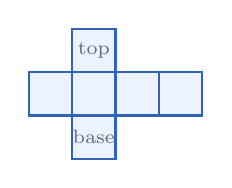
\begin{tikzpicture}[scale=0.55]
\foreach \x/\y in {1/2,0/1,1/1,2/1,3/1,1/0}{\draw[geo,fill=tmBlue!10] (\x,\y) rectangle ++(1,1);}
\node[dim] at (1.5,2.5){top}; \node[dim] at (1.5,0.5){base};
\end{tikzpicture}\qquad
\begin{tikzpicture}[scale=0.6]
\cuboidVT{1.6}{1.6}{1.6}{0}
\node[dim,below] at ($(Q)!0.5!(P)$){$a$};
\end{tikzpicture}
\end{minipage}
\end{knowbox}
\shead{Lateral area and total surface area}
\begin{knowbox}
The \textbf{lateral area} $S_{\text{lat}}$ of a cuboid is the total area of its $4$ side faces. Unfolded, the four side faces make one long rectangle whose length is the \textbf{perimeter of the base} and whose width is the \textbf{height}:
\[S_{\text{lat}}=(a+b)\times2\times c\qquad(\text{perimeter of base}\times\text{height})\]
The \textbf{total surface area} $S_{\text{tot}}$ is the lateral area plus the areas of the two bases:
\[S_{\text{tot}}=S_{\text{lat}}+a\times b\times2\]
For a \textbf{cube} with edge $a$: \quad $S_{\text{lat}}=a\times a\times4,\qquad S_{\text{tot}}=a\times a\times6.$\par
\smallskip
\emph{Remember:} all dimensions must be in the same unit. A box \emph{without a lid} has only one base: its area is $S_{\text{lat}}+a\times b$.
\end{knowbox}
\gap
\begin{exbox}{\ExWord\ 1}
A cuboid is $8$ cm long, $5$ cm wide and $6$ cm high. Find:
\begin{cols3}
\pa{a} its lateral area; & \pa{b} the area of one base; & \pa{c} its total surface area.
\end{cols3}
\guide
\pa{a} Perimeter of the base: $(8+5)\times2=26$ cm.\par $S_{\text{lat}}=26\times6=156$ cm$^2$.\par
\pa{b} Area of one base: $8\times5=40$ cm$^2$.\par
\pa{c} $S_{\text{tot}}=156+40\times2=236$ cm$^2$.
\dapso{\pa{a} $156$ cm$^2$; \pa{b} $40$ cm$^2$; \pa{c} $236$ cm$^2$.}
\end{exbox}
\gap
\begin{exbox}{\ExWord\ 2}
A cube has a total surface area of $294$ cm$^2$. Find its edge and its lateral area.
\guide
A cube has $6$ equal faces. Area of one face: $294:6=49$ cm$^2$.\par
Since $49=7\times7$, the edge is $7$ cm.\par
Lateral area: $49\times4=196$ cm$^2$.
\dapso{Edge $7$ cm; $196$ cm$^2$.}
\end{exbox}
\gap
\begin{exbox}{\ExWord\ 3}
A cuboid has a base of area $60$ cm$^2$. Its length is $3$ times its height and is $8$ cm more than its height. Find its lateral area and total surface area.
\guide
The length is $3$ times the height, so the difference is $3-1=2$ times the height.\par
Height: $8:2=4$ cm.\quad Length: $4\times3=12$ cm.\quad Width: $60:12=5$ cm.\par
$S_{\text{lat}}=(12+5)\times2\times4=136$ cm$^2$.\par
$S_{\text{tot}}=136+60\times2=256$ cm$^2$.
\dapso{$136$ cm$^2$; $256$ cm$^2$.}
\end{exbox}
\gap
\begin{exbox}{\ExWord\ 4}
\begin{minipage}[t]{0.6\linewidth}
A tin box \emph{without a lid} is $50$ cm long, $30$ cm wide and $20$ cm high. How much tin is needed to make it? (Ignore the seams.)
\end{minipage}\hfill
\begin{minipage}[t]{0.36\linewidth}\vspace{0pt}\centering
\begin{tikzpicture}[scale=0.42]
\cuboidVT{5}{3}{2}{0}
\fill[white] (D)--(C)--(B)--(A)--cycle; \draw[geo] (D)--(C)--(B)--(A)--cycle;
\node[dim,below] at ($(Q)!0.5!(P)$){$50$ cm}; \node[dim,right] at ($(P)!0.5!(N)$){$30$ cm}; \node[dim,left] at ($(Q)!0.5!(D)$){$20$ cm};
\end{tikzpicture}
\end{minipage}
\guide
The box has $4$ side faces and only $1$ base.\par
Lateral area: $(50+30)\times2\times20=3\,200$ cm$^2$.\par
Base: $50\times30=1\,500$ cm$^2$.\par
Tin needed: $3\,200+1\,500=4\,700$ cm$^2$.
\dapso{$4\,700$ cm$^2$.}
\end{exbox}
\gap
\begin{exbox}{\ExWord\ 5}
A room is $6$ m long, $4.5$ m wide and $3.5$ m high. The four walls and the ceiling are to be painted. The doors and windows have a total area of $7.5$ m$^2$. Find the area to be painted.
\guide
Four walls (lateral area): $(6+4.5)\times2\times3.5=73.5$ m$^2$.\par
Ceiling: $6\times4.5=27$ m$^2$.\par
Area to paint: $73.5+27-7.5=93$ m$^2$.
\note{The floor is not painted, and the doors and windows are taken away.}
\dapso{$93$ m$^2$.}
\end{exbox}
\dividerbar{Practice}
\begin{probbox}{1}{\relax}
\begin{minipage}[t]{0.58\linewidth}
Cuboid ABCD.MNPQ has $QP=7$ cm, $QM=4$ cm and $QD=5$ cm.\par
\pa{a} Find the lengths of the edges AB, BN and NP.\par
\pa{b} Find the areas of the base MNPQ and of the faces DCPQ and ADQM.\par
\pa{c} Find its lateral area and total surface area.
\end{minipage}\hfill
\begin{minipage}[t]{0.38\linewidth}\vspace{0pt}\centering
\begin{tikzpicture}[scale=0.5]
\cuboidVT{4.2}{3.2}{3}{0}
\node[lbl,above left] at (A){A}; \node[lbl,above right] at (B){B}; \node[lbl,right] at (C){C}; \node[lbl,left] at (D){D};
\node[lbl,above left] at (M){M}; \node[lbl,right] at (N){N}; \node[lbl,below right] at (P){P}; \node[lbl,below left] at (Q){Q};
\node[dim,below] at ($(Q)!0.5!(P)$){$7$ cm}; \node[dim,left] at ($(Q)!0.5!(D)$){$5$ cm}; \node[dim,right] at ($(Q)!0.45!(M)$){$4$ cm};
\end{tikzpicture}
\end{minipage}
\end{probbox}
\probsol{
\pa{a} $AB=QP=7$ cm; $BN=QD=5$ cm; $NP=QM=4$ cm.\par
\pa{b} $S_{MNPQ}=7\times4=28$ cm$^2$; $S_{DCPQ}=7\times5=35$ cm$^2$; $S_{ADQM}=4\times5=20$ cm$^2$.\par
\pa{c} $S_{\text{lat}}=(7+4)\times2\times5=110$ cm$^2$.\par $S_{\text{tot}}=110+28\times2=166$ cm$^2$.
\dapso{\pa{a} $7$ cm, $5$ cm, $4$ cm;\par \pa{b} $28$ cm$^2$, $35$ cm$^2$, $20$ cm$^2$;\par \pa{c} $110$ cm$^2$, $166$ cm$^2$.}}
\gap
\begin{probbox}{2}{\relax}
Which of the figures below are nets of a cube?\par\smallskip
\begin{center}
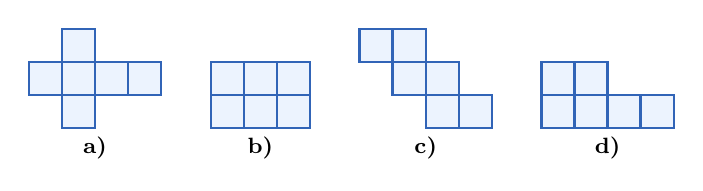
\begin{tikzpicture}[scale=0.42]
\foreach \x/\y in {1/2,0/1,1/1,2/1,3/1,1/0}{\draw[geo,fill=tmBlue!10] (\x,\y) rectangle ++(1,1);}
\node[lbl] at (2,-0.6){\pa{a}};
\begin{scope}[xshift=5.5cm]
\foreach \x/\y in {0/0,1/0,2/0,0/1,1/1,2/1}{\draw[geo,fill=tmBlue!10] (\x,\y) rectangle ++(1,1);}
\node[lbl] at (1.5,-0.6){\pa{b}};
\end{scope}
\begin{scope}[xshift=10cm]
\foreach \x/\y in {0/2,1/2,1/1,2/1,2/0,3/0}{\draw[geo,fill=tmBlue!10] (\x,\y) rectangle ++(1,1);}
\node[lbl] at (2,-0.6){\pa{c}};
\end{scope}
\begin{scope}[xshift=15.5cm]
\foreach \x/\y in {0/0,1/0,2/0,3/0,0/1,1/1}{\draw[geo,fill=tmBlue!10] (\x,\y) rectangle ++(1,1);}
\node[lbl] at (2,-0.6){\pa{d}};
\end{scope}
\end{tikzpicture}
\end{center}
\end{probbox}
\probsol{
\pa{a} The row of $4$ squares folds into the $4$ side faces; the square above is the top and the square below is the base. It is a net.\par
\pa{b} Folding the $2\times3$ block, the squares overlap and two faces stay open. It is not a net.\par
\pa{c} This ``staircase'' folds into a cube with no overlap. It is a net.\par
\pa{d} The two squares on top of the row both become the same end face, and the other end stays open. It is not a net.
\dapso{Figures \textbf{a)} and \textbf{c)}.}}
\gap
\begin{probbox}{3}{\relax}
Find the lateral area and the total surface area of a cuboid with:
\begin{cols2}
\pa{a} $a=9$ cm, $b=6$ cm, $c=5$ cm; & \pa{b} $a=2.5$ m, $b=1.5$ m, $c=1.2$ m;\\
\pa{c} $a=\dfrac45$ m, $b=\dfrac12$ m, $c=\dfrac13$ m; & \pa{d} $a=1.2$ dm, $b=8$ cm, $c=5$ cm.
\end{cols2}
\end{probbox}
\probsol{
\pa{a} $S_{\text{lat}}=(9+6)\times2\times5=150$ cm$^2$; $S_{\text{tot}}=150+9\times6\times2=258$ cm$^2$.\par
\pa{b} $S_{\text{lat}}=(2.5+1.5)\times2\times1.2=9.6$ m$^2$; $S_{\text{tot}}=9.6+2.5\times1.5\times2=17.1$ m$^2$.\par
\pa{c} $S_{\text{lat}}=\left(\dfrac45+\dfrac12\right)\times2\times\dfrac13=\dfrac{13}{10}\times\dfrac23=\dfrac{13}{15}$ m$^2$;\par
$S_{\text{tot}}=\dfrac{13}{15}+\dfrac45\times\dfrac12\times2=\dfrac{13}{15}+\dfrac{12}{15}=\dfrac53$ m$^2$.\par
\pa{d} $1.2$ dm $=12$ cm. $S_{\text{lat}}=(12+8)\times2\times5=200$ cm$^2$; $S_{\text{tot}}=200+12\times8\times2=392$ cm$^2$.
\dapso{\pa{a} $150$ cm$^2$, $258$ cm$^2$;\par \pa{b} $9.6$ m$^2$, $17.1$ m$^2$;\par \pa{c} $\dfrac{13}{15}$ m$^2$, $\dfrac53$ m$^2$;\par \pa{d} $200$ cm$^2$, $392$ cm$^2$.}}
\gap
\begin{probbox}{4}{\relax}
Find the lateral area and the total surface area of a cube with edge:
\begin{cols3}
\pa{a} $6$ cm; & \pa{b} $2.5$ dm; & \pa{c} $\dfrac34$ m.
\end{cols3}
\end{probbox}
\probsol{
\pa{a} $S_{\text{lat}}=6\times6\times4=144$ cm$^2$; $S_{\text{tot}}=6\times6\times6=216$ cm$^2$.\par
\pa{b} $S_{\text{lat}}=2.5\times2.5\times4=25$ dm$^2$; $S_{\text{tot}}=2.5\times2.5\times6=37.5$ dm$^2$.\par
\pa{c} $S_{\text{lat}}=\dfrac34\times\dfrac34\times4=\dfrac94$ m$^2$; $S_{\text{tot}}=\dfrac34\times\dfrac34\times6=\dfrac{27}8$ m$^2$.
\dapso{\pa{a} $144$ cm$^2$, $216$ cm$^2$;\par \pa{b} $25$ dm$^2$, $37.5$ dm$^2$;\par \pa{c} $\dfrac94$ m$^2$, $\dfrac{27}8$ m$^2$.}}
\gap
\begin{probbox}{5}{\relax}
A cuboid is $15$ cm long, $10$ cm wide and $8$ cm high. Find:
\begin{cols3}
\pa{a} the perimeter of its base; & \pa{b} its lateral area; & \pa{c} its total surface area.
\end{cols3}
\end{probbox}
\probsol{
\pa{a} $(15+10)\times2=50$ cm.\par
\pa{b} $50\times8=400$ cm$^2$.\par
\pa{c} $400+15\times10\times2=700$ cm$^2$.
\dapso{\pa{a} $50$ cm; \pa{b} $400$ cm$^2$; \pa{c} $700$ cm$^2$.}}
\gap
\begin{probbox}{6}{\relax}
Mai wraps a gift box $24$ cm long, $16$ cm wide and $10$ cm high, covering every face. What is the least area of wrapping paper she needs?
\end{probbox}
\probsol{
The paper must cover all $6$ faces, i.e.\ the total surface area.\par
$S_{\text{lat}}=(24+16)\times2\times10=800$ cm$^2$.\par
$S_{\text{tot}}=800+24\times16\times2=1\,568$ cm$^2$.
\dapso{$1\,568$ cm$^2$.}}
\gap
\begin{probbox}{7}{\relax}
A box is $40$ cm long, $25$ cm wide and $20$ cm high. Lan covers its four side faces with blue paper and its two bases with yellow paper (outside only). Which colour of paper is used more, and by how many square centimetres?
\end{probbox}
\probsol{
Blue paper (lateral area): $(40+25)\times2\times20=2\,600$ cm$^2$.\par
Yellow paper (two bases): $40\times25\times2=2\,000$ cm$^2$.\par
Blue is more by $2\,600-2\,000=600$ cm$^2$.
\dapso{Blue paper, by $600$ cm$^2$.}}
\gap
\begin{probbox}{8}{\relax}
An iron box without a lid is $60$ cm long, $40$ cm wide and $30$ cm high. How much iron sheet is used to make it? (Ignore the seams.)
\end{probbox}
\probsol{
Lateral area: $(60+40)\times2\times30=6\,000$ cm$^2$.\par
Base: $60\times40=2\,400$ cm$^2$.\par
Iron sheet: $6\,000+2\,400=8\,400$ cm$^2$.
\dapso{$8\,400$ cm$^2$.}}
\gap
\begin{probbox}{9}{\relax}
A classroom is $8$ m long, $6$ m wide and $3.5$ m high. The four walls and the ceiling are to be painted; the doors and windows cover $9.5$ m$^2$. Find the area to be painted.
\end{probbox}
\probsol{
Walls: $(8+6)\times2\times3.5=98$ m$^2$.\par
Ceiling: $8\times6=48$ m$^2$.\par
Area to paint: $98+48-9.5=136.5$ m$^2$.
\dapso{$136.5$ m$^2$.}}
\gap
\begin{probbox}{10}{\relax}
A water tank in the shape of a cube without a lid has edge $1.5$ m. Its outside (side faces and bottom) is painted. Find the painted area.
\end{probbox}
\probsol{
One face: $1.5\times1.5=2.25$ m$^2$.\par
A cube without a lid has $5$ faces: $2.25\times5=11.25$ m$^2$.
\dapso{$11.25$ m$^2$.}}
\gap
\begin{probbox}{11}{\relax}
A cube has a lateral area of $100$ cm$^2$. Find its edge and its total surface area.
\end{probbox}
\probsol{
One face: $100:4=25$ cm$^2$; since $25=5\times5$, the edge is $5$ cm.\par
$S_{\text{tot}}=25\times6=150$ cm$^2$.
\dapso{$5$ cm; $150$ cm$^2$.}}
\gap
\begin{probbox}{12}{\relax}
A cube has a total surface area of $600$ cm$^2$. Find its lateral area.
\end{probbox}
\probsol{
One face: $600:6=100$ cm$^2$.\par
$S_{\text{lat}}=100\times4=400$ cm$^2$.
\dapso{$400$ cm$^2$.}}
\gap
\begin{probbox}{13}{\relax}
A cube has a lateral area of $1.44$ m$^2$. Find its edge and its total surface area.
\end{probbox}
\probsol{
One face: $1.44:4=0.36$ m$^2$; since $0.36=0.6\times0.6$, the edge is $0.6$ m.\par
$S_{\text{tot}}=0.36\times6=2.16$ m$^2$.
\dapso{$0.6$ m; $2.16$ m$^2$.}}
\gap
\begin{probbox}{14}{\relax}
A cuboid has a lateral area of $360$ cm$^2$ and a height of $9$ cm. Its length is $4$ cm more than its width. Find the length and the width.
\end{probbox}
\probsol{
Perimeter of the base: $360:9=40$ cm.\par
Length $+$ width: $40:2=20$ cm.\par
Length: $(20+4):2=12$ cm.\quad Width: $20-12=8$ cm.
\dapso{Length $12$ cm, width $8$ cm.}}
\gap
\begin{probbox}{15}{\relax}
A cuboid has a base perimeter of $36$ dm and a height of $7$ dm. Find its lateral area.
\end{probbox}
\probsol{
$S_{\text{lat}}=36\times7=252$ dm$^2$.
\dapso{$252$ dm$^2$.}}
\gap
\begin{probbox}{16}{\relax}
A cuboid has a lateral area of $480$ cm$^2$ and a base perimeter of $48$ cm. Find its height.
\end{probbox}
\probsol{
Height $=$ lateral area $:$ perimeter of base.\par
$c=480:48=10$ cm.
\dapso{$10$ cm.}}
\gap
\begin{probbox}{17}{\relax}
A cuboid is $2.4$ m long and $1.6$ m wide, and its total surface area is $19.68$ m$^2$. Find its height.
\end{probbox}
\probsol{
Two bases: $2.4\times1.6\times2=7.68$ m$^2$.\par
Lateral area: $19.68-7.68=12$ m$^2$.\par
Perimeter of base: $(2.4+1.6)\times2=8$ m.\par
Height: $12:8=1.5$ m.
\dapso{$1.5$ m.}}
\gap
\begin{probbox}{18}{\relax}
A wooden crate is $1.2$ m long, $0.8$ m wide and $0.6$ m high. All of its outside faces are varnished, using $0.25$ kg of varnish per square metre. How many kilograms of varnish are needed?
\end{probbox}
\probsol{
$S_{\text{lat}}=(1.2+0.8)\times2\times0.6=2.4$ m$^2$.\par
$S_{\text{tot}}=2.4+1.2\times0.8\times2=4.32$ m$^2$.\par
Varnish: $0.25\times4.32=1.08$ kg.
\dapso{$1.08$ kg.}}
\gap
\begin{probbox}{19}{\relax}
A swimming pool is $25$ m long, $10$ m wide and $1.6$ m deep. Its bottom and its four walls are covered with tiles measuring $25$ cm by $20$ cm. How many tiles are needed? (Ignore the joints.)
\end{probbox}
\probsol{
Walls: $(25+10)\times2\times1.6=112$ m$^2$.\quad Bottom: $25\times10=250$ m$^2$.\par
Area to tile: $112+250=362$ m$^2$.\par
One tile: $25\times20=500$ cm$^2$ $=0.05$ m$^2$.\par
Tiles: $362:0.05=7\,240$ tiles.
\dapso{$7\,240$ tiles.}}
\gap
\begin{probbox}{20}{\relax}
A fish pond is $3$ m long, $2$ m wide and $0.8$ m deep. Its bottom and walls are covered with square tiles of side $2$ dm. How many tiles are needed?
\end{probbox}
\probsol{
Walls: $(3+2)\times2\times0.8=8$ m$^2$.\quad Bottom: $3\times2=6$ m$^2$.\par
Area to tile: $8+6=14$ m$^2$ $=1\,400$ dm$^2$.\par
One tile: $2\times2=4$ dm$^2$.\quad Tiles: $1\,400:4=350$.
\dapso{$350$ tiles.}}
\gap
\begin{probbox}{21}{\relax}
A cuboid has a base perimeter of $30$ cm; its length is $3$ cm more than its width, and its height is $\dfrac23$ of its length. Find its lateral area and total surface area.
\end{probbox}
\probsol{
Length $+$ width: $30:2=15$ cm.\par
Length: $(15+3):2=9$ cm.\quad Width: $6$ cm.\quad Height: $9\times\dfrac23=6$ cm.\par
$S_{\text{lat}}=30\times6=180$ cm$^2$.\par
$S_{\text{tot}}=180+9\times6\times2=288$ cm$^2$.
\dapso{$180$ cm$^2$; $288$ cm$^2$.}}
\gap
\begin{probbox}{22}{\relax}
Compare the total surface area of a cube with edge $6$ cm and that of a cuboid $8$ cm long, $6$ cm wide and $4$ cm high.
\end{probbox}
\probsol{
Cube: $6\times6\times6=216$ cm$^2$.\par
Cuboid: $(8+6)\times2\times4+8\times6\times2=112+96=208$ cm$^2$.\par
$216-208=8$ cm$^2$.
\dapso{The cube's is larger, by $8$ cm$^2$.}}
\gap
\begin{probbox}{23}{\relax}
A cuboid has a square base of side $5$ cm and a height of $12$ cm. Find its lateral area and total surface area.
\end{probbox}
\probsol{
Perimeter of base: $5\times4=20$ cm.\par
$S_{\text{lat}}=20\times12=240$ cm$^2$.\par
$S_{\text{tot}}=240+5\times5\times2=290$ cm$^2$.
\dapso{$240$ cm$^2$; $290$ cm$^2$.}}
\gap
\begin{probbox}{24}{\relax}
A lantern has a frame in the shape of a cuboid with a square base of side $20$ cm and a height of $35$ cm. Paper is glued on the four sides and the bottom. How many square decimetres of paper are used?
\end{probbox}
\probsol{
Four sides: $20\times4\times35=2\,800$ cm$^2$.\par
Bottom: $20\times20=400$ cm$^2$.\par
Paper: $2\,800+400=3\,200$ cm$^2$ $=32$ dm$^2$.
\dapso{$32$ dm$^2$.}}
\gap
\begin{probbox}{25}{\relax}
A piece of cardboard is just enough to make a cube-shaped box without a lid, with edge $2.5$ dm. Find the area of the cardboard. (Ignore the flaps.)
\end{probbox}
\probsol{
One face: $2.5\times2.5=6.25$ dm$^2$.\par
The box has $5$ faces: $6.25\times5=31.25$ dm$^2$.
\dapso{$31.25$ dm$^2$.}}
\gap
\begin{probbox}{26}{\relax}
A cube-shaped tank without a lid has a base perimeter of $4.8$ m. Both its inside and its outside are painted, and $1$ kg of paint covers $3$ m$^2$. How many kilograms of paint are needed?
\end{probbox}
\probsol{
Edge: $4.8:4=1.2$ m.\quad One face: $1.2\times1.2=1.44$ m$^2$.\par
Without a lid there are $5$ faces, painted on both sides: $1.44\times5\times2=14.4$ m$^2$.\par
Paint: $14.4:3=4.8$ kg.
\dapso{$4.8$ kg.}}
\gap
\begin{probbox}{27}{\relax}
The $12$ edges of a cuboid add up to $96$ cm. Its length is $12$ cm and its width is $8$ cm. Find its total surface area.
\end{probbox}
\probsol{
A cuboid has $4$ lengths, $4$ widths and $4$ heights.\par
Length $+$ width $+$ height: $96:4=24$ cm.\quad Height: $24-12-8=4$ cm.\par
$S_{\text{lat}}=(12+8)\times2\times4=160$ cm$^2$.\par
$S_{\text{tot}}=160+12\times8\times2=352$ cm$^2$.
\dapso{$352$ cm$^2$.}}
\gap
\begin{probbox}{28}{\relax}
The $12$ edges of a cube add up to $72$ cm. Find its total surface area.
\end{probbox}
\probsol{
Edge: $72:12=6$ cm.\par
$S_{\text{tot}}=6\times6\times6=216$ cm$^2$.
\dapso{$216$ cm$^2$.}}
\gap
\begin{probbox}{29}{\relax}
A glass aquarium without a lid is $80$ cm long, $40$ cm wide and $50$ cm high. How many square decimetres of glass are used?
\end{probbox}
\probsol{
Four walls: $(80+40)\times2\times50=12\,000$ cm$^2$.\par
Bottom: $80\times40=3\,200$ cm$^2$.\par
Glass: $12\,000+3\,200=15\,200$ cm$^2$ $=152$ dm$^2$.
\dapso{$152$ dm$^2$.}}
\gap
\begin{probbox}{30}{\relax}
The total surface area of a cube is $50$ cm$^2$ more than its lateral area. Find its lateral area.
\end{probbox}
\probsol{
The difference is the area of the two bases: one face is $50:2=25$ cm$^2$.\par
$S_{\text{lat}}=25\times4=100$ cm$^2$.
\dapso{$100$ cm$^2$.}}
\dividerbar{Challenge -- Extension}
\begin{probbox}{31}{\stars{1}}
A cuboid has a base of area $120$ cm$^2$. Its length is $9$ cm more than its height, and its height is $\dfrac25$ of its length. Find its lateral area and total surface area.
\end{probbox}
\probsol{
Height $2$ parts, length $5$ parts; the difference is $3$ parts $=9$ cm, so $1$ part is $3$ cm.\par
Height: $3\times2=6$ cm.\quad Length: $3\times5=15$ cm.\quad Width: $120:15=8$ cm.\par
$S_{\text{lat}}=(15+8)\times2\times6=276$ cm$^2$.\par
$S_{\text{tot}}=276+120\times2=516$ cm$^2$.
\dapso{$276$ cm$^2$; $516$ cm$^2$.}}
\gap
\begin{probbox}{32}{\stars{1}}
A water tank has a lateral area of $10.5$ m$^2$ and a height of $1.5$ m. Its length is $1$ m more than its width. Find its length and width.
\end{probbox}
\probsol{
Perimeter of base: $10.5:1.5=7$ m.\quad Length $+$ width: $7:2=3.5$ m.\par
Length: $(3.5+1):2=2.25$ m.\quad Width: $3.5-2.25=1.25$ m.
\dapso{Length $2.25$ m, width $1.25$ m.}}
\gap
\begin{probbox}{33}{\stars{1}}
An iron crate in the shape of a cuboid has a width equal to $\dfrac34$ of its length and $0.5$ m less than its length; its height is $1.2$ m.\par
\pa{a} Find its total surface area.\par
\pa{b} The outside is painted completely, using $3$ kg of paint for every $4$ m$^2$. How many kilograms of paint are needed?
\end{probbox}
\probsol{
\pa{a} Length $4$ parts, width $3$ parts; the difference is $1$ part $=0.5$ m.\par
Length: $0.5\times4=2$ m.\quad Width: $0.5\times3=1.5$ m.\par
$S_{\text{lat}}=(2+1.5)\times2\times1.2=8.4$ m$^2$.\quad $S_{\text{tot}}=8.4+2\times1.5\times2=14.4$ m$^2$.\par
\pa{b} $1$ m$^2$ needs $3:4=0.75$ kg. Paint: $0.75\times14.4=10.8$ kg.
\dapso{\pa{a} $14.4$ m$^2$; \pa{b} $10.8$ kg.}}
\gap
\begin{probbox}{34}{\stars{2}}
If the edge of a cube is increased by $2$ cm, its total surface area increases by $120$ cm$^2$. Find the original edge.
\end{probbox}
\probsol{
Each of the $6$ faces grows by $120:6=20$ cm$^2$.\par
A square of side $a$ becomes a square of side $a+2$: the new part is two strips $a$ by $2$ and a corner square $2$ by $2$.\par
$a\times2\times2+2\times2=20$, so $a\times4=16$ and $a=4$ cm.\par
\emph{Check:} $6\times6\times6-4\times4\times6=216-96=120$ cm$^2$.
\dapso{$4$ cm.}}
\gap
\begin{probbox}{35}{\stars{1}}
Two cubes, each with edge $5$ cm, are glued face to face to make a cuboid. Find the total surface area of the cuboid. How much less is it than the total of the two cubes' surface areas?
\end{probbox}
\probsol{
The cuboid is $10$ cm $\times\,5$ cm $\times\,5$ cm.\par
$S_{\text{tot}}=(10+5)\times2\times5+10\times5\times2=150+100=250$ cm$^2$.\par
Two cubes: $5\times5\times6\times2=300$ cm$^2$.\par
Less by $300-250=50$ cm$^2$: the two glued faces ($2\times25$ cm$^2$) are hidden.
\dapso{$250$ cm$^2$; $50$ cm$^2$ less.}}
\gap
\begin{probbox}{36}{\stars{1}}
Three cubes with edge $4$ cm are put in a row and glued into a cuboid. Find the total surface area of that cuboid.
\end{probbox}
\probsol{
The cuboid is $12$ cm $\times\,4$ cm $\times\,4$ cm.\par
$S_{\text{tot}}=(12+4)\times2\times4+12\times4\times2=128+96=224$ cm$^2$.\par
\emph{Other way:} the $3$ cubes have $18$ faces; each of the $2$ joints hides $2$ faces, so $18-4=14$ faces remain: $14\times4\times4=224$ cm$^2$.
\dapso{$224$ cm$^2$.}}
\gap
\begin{probbox}{37}{\stars{1}}
A cuboid $10$ cm long, $6$ cm wide and $4$ cm high is cut into two equal halves by a cut parallel to its base. Find the total surface area of the original cuboid and the total surface area of the two halves together.
\end{probbox}
\probsol{
Original: $(10+6)\times2\times4+10\times6\times2=128+120=248$ cm$^2$.\par
The cut makes two new faces, each $10\times6=60$ cm$^2$.\par
Two halves together: $248+60\times2=368$ cm$^2$.
\dapso{$248$ cm$^2$; $368$ cm$^2$.}}
\gap
\begin{probbox}{38}{\stars{1}}
A cuboid has a square base and a lateral area of $160$ cm$^2$. Its height is $2.5$ times the side of the base. Find its total surface area.
\end{probbox}
\probsol{
Each side face is a rectangle (base side) $\times$ ($2.5\times$ base side), so it equals $2.5$ squares of the base.\par
Lateral area $=4\times2.5=10$ base squares: one base square is $160:10=16$ cm$^2$ (side $4$ cm, height $10$ cm).\par
$S_{\text{tot}}=160+16\times2=192$ cm$^2$.
\dapso{$192$ cm$^2$.}}
\gap
\begin{probbox}{39}{\stars{1}}
A cube has a total surface area of $1.5$ m$^2$. Find its edge and its lateral area.
\end{probbox}
\probsol{
One face: $1.5:6=0.25$ m$^2$; since $0.25=0.5\times0.5$, the edge is $0.5$ m.\par
$S_{\text{lat}}=0.25\times4=1$ m$^2$.
\dapso{$0.5$ m; $1$ m$^2$.}}
\gap
\begin{probbox}{40}{\stars{2}}
\begin{minipage}[t]{0.6\linewidth}
From a rectangular sheet of card $40$ cm by $30$ cm, Nam cuts a square of side $5$ cm from each corner and folds up the sides to make an open box. Find the length, width and height of the box and the area of card it uses.
\end{minipage}\hfill
\begin{minipage}[t]{0.36\linewidth}\vspace{0pt}\centering
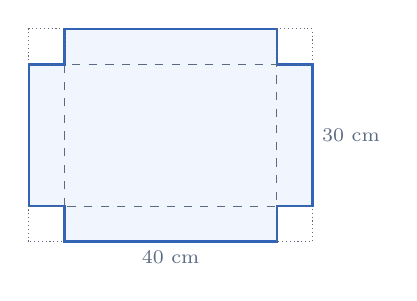
\begin{tikzpicture}[scale=0.09]
\draw[geo,fill=tmBlue!8] (5,0)--(35,0)--(35,5)--(40,5)--(40,25)--(35,25)--(35,30)--(5,30)--(5,25)--(0,25)--(0,5)--(5,5)--cycle;
\draw[dashed,Slate] (5,5) rectangle (35,25);
\foreach \x/\y in {0/0,35/0,0/25,35/25}{\draw[Slate,densely dotted] (\x,\y) rectangle ++(5,5);}
\node[dim,below] at (20,0){$40$ cm}; \node[dim,right] at (40,15){$30$ cm};
\end{tikzpicture}
\end{minipage}
\end{probbox}
\probsol{
Length: $40-5\times2=30$ cm.\quad Width: $30-5\times2=20$ cm.\quad Height: $5$ cm.\par
Card used: $40\times30-5\times5\times4=1\,200-100=1\,100$ cm$^2$.\par
\emph{Check:} $S_{\text{lat}}+$ base $=(30+20)\times2\times5+30\times20=500+600=1\,100$ cm$^2$.
\dapso{$30$ cm, $20$ cm, $5$ cm; $1\,100$ cm$^2$.}}
\gap
\begin{probbox}{41}{\stars{1}}
A room is $5$ m long, $4$ m wide and $3$ m high. The inside walls and the ceiling are painted. The door and windows cover $4$ m$^2$. Painting costs $25\,000$ đồng per square metre. Find the cost.
\end{probbox}
\probsol{
Walls: $(5+4)\times2\times3=54$ m$^2$.\quad Ceiling: $5\times4=20$ m$^2$.\par
Area to paint: $54+20-4=70$ m$^2$.\par
Cost: $25\,000\times70=1\,750\,000$ đồng.
\dapso{$1\,750\,000$ đồng.}}
\gap
\begin{probbox}{42}{\stars{1}}
The $12$ edges of a cuboid add up to $120$ cm. Its length is $3$ times its width and its height is $2$ times its width. Find its total surface area.
\end{probbox}
\probsol{
Length $+$ width $+$ height: $120:4=30$ cm $=3+1+2=6$ widths.\par
Width: $30:6=5$ cm.\quad Length: $15$ cm.\quad Height: $10$ cm.\par
$S_{\text{tot}}=(15+5)\times2\times10+15\times5\times2=400+150=550$ cm$^2$.
\dapso{$550$ cm$^2$.}}
\gap
\begin{probbox}{43}{\stars{2}}
Three different faces of a cuboid have areas $12$ cm$^2$, $15$ cm$^2$ and $20$ cm$^2$. Find its total surface area, and find its three dimensions (whole numbers of centimetres).
\end{probbox}
\probsol{
Each face appears twice: $S_{\text{tot}}=(12+15+20)\times2=94$ cm$^2$.\par
Try whole numbers: the edge shared by the faces $12$ and $15$ divides both, so it is $1$ or $3$.\par
If it is $3$: the other edges are $12:3=4$ and $15:3=5$, and $4\times5=20$. \checkmark\par
(If it were $1$: $12\times15=180\neq20$.)
\dapso{$94$ cm$^2$; $3$ cm, $4$ cm, $5$ cm.}}
\gap
\begin{probbox}{44}{\stars{1}}
A cube-shaped box without a lid has edge $15$ cm. Coloured paper is glued on both the inside and the outside. Find the area of paper used.
\end{probbox}
\probsol{
One face: $15\times15=225$ cm$^2$.\par
$5$ faces, both sides: $225\times5\times2=2\,250$ cm$^2$.
\dapso{$2\,250$ cm$^2$.}}
\gap
\begin{probbox}{45}{\stars{1}}
A cuboid has a square base of side $6$ cm. Its lateral area is $3$ times the total area of its two bases. Find its height and total surface area.
\end{probbox}
\probsol{
Two bases: $6\times6\times2=72$ cm$^2$.\par
$S_{\text{lat}}=72\times3=216$ cm$^2$.\quad Height: $216:(6\times4)=9$ cm.\par
$S_{\text{tot}}=216+72=288$ cm$^2$.
\dapso{$9$ cm; $288$ cm$^2$.}}
\gap
\begin{probbox}{46}{\stars{1}}
Two identical cuboids, each $8$ cm $\times\,5$ cm $\times\,3$ cm, are glued together along their largest faces. Find the total surface area of the new cuboid.
\end{probbox}
\probsol{
The largest face is $8\times5=40$ cm$^2$. The new cuboid is $8$ cm $\times\,5$ cm $\times\,6$ cm.\par
$S_{\text{tot}}=(8+5)\times2\times6+8\times5\times2=156+80=236$ cm$^2$.\par
\emph{Check:} one cuboid has $(8+5)\times2\times3+80=158$ cm$^2$; $158\times2-40\times2=236$ cm$^2$.
\dapso{$236$ cm$^2$.}}
\gap
\begin{probbox}{47}{\stars{2}}
A pool is $12.5$ m long, $6$ m wide and $1.4$ m deep. Its bottom and walls are tiled with tiles of $25$ cm $\times\,20$ cm. Tiles are sold in boxes of $12$. How many boxes must be bought?
\end{probbox}
\probsol{
Walls: $(12.5+6)\times2\times1.4=51.8$ m$^2$.\quad Bottom: $12.5\times6=75$ m$^2$.\par
Area: $51.8+75=126.8$ m$^2$.\quad One tile: $0.05$ m$^2$.\par
Tiles: $126.8:0.05=2\,536$.\par
$2\,536:12=211$ remainder $4$, so $211$ boxes are not enough; we need $212$ boxes.
\dapso{$212$ boxes.}}
\gap
\begin{probbox}{48}{\stars{1}}
A cube has the same total surface area as a cuboid $12$ cm long, $9$ cm wide and $4$ cm high. Find the edge of the cube.
\end{probbox}
\probsol{
Cuboid: $(12+9)\times2\times4+12\times9\times2=168+216=384$ cm$^2$.\par
One face of the cube: $384:6=64$ cm$^2$ $=8\times8$.
\dapso{$8$ cm.}}
\gap
\begin{probbox}{49}{\stars{2}}
A cuboid is $5$ cm high. If its length is decreased by $3$ cm and its width increased by $3$ cm, its base becomes a square of side $8$ cm. Compare the total surface areas of the old and the new cuboid.
\end{probbox}
\probsol{
Old length: $8+3=11$ cm.\quad Old width: $8-3=5$ cm.\par
Base perimeter does not change ($32$ cm), so the lateral area is the same: $32\times5=160$ cm$^2$.\par
Old: $160+11\times5\times2=270$ cm$^2$.\quad New: $160+8\times8\times2=288$ cm$^2$.\par
The new one is larger by $18$ cm$^2$.
\dapso{The new cuboid's is larger, by $18$ cm$^2$.}}
\gap
\begin{probbox}{50}{\stars{2}}
A cube of edge $6$ cm is cut into $8$ equal small cubes. Find the total surface area of the $8$ small cubes and compare it with that of the big cube.
\end{probbox}
\probsol{
Each small cube has edge $6:2=3$ cm.\par
One small cube: $3\times3\times6=54$ cm$^2$.\quad $8$ cubes: $54\times8=432$ cm$^2$.\par
Big cube: $6\times6\times6=216$ cm$^2$.\quad $432:216=2$.
\dapso{$432$ cm$^2$, twice as much.}}
\clearpage
\titlehead
\begingroup\setbox0=\vbox{\section*{Volume}}\endgroup
\chapterhead{4}{Volume}
\shead{Volume and units of volume}
\gdef\cuboidVT#1#2#3#4{\coordinate (Q) at (0,0); \coordinate (P) at (#1,0); \coordinate (C) at (#1,#3); \coordinate (D) at (0,#3);
 \coordinate (M) at ({0.5*#2},{0.38*#2}); \coordinate (N) at ($(P)+(M)$); \coordinate (B) at ($(C)+(M)$); \coordinate (A) at ($(D)+(M)$);
 \fill[tmBlue!6] (Q)--(P)--(C)--(D)--cycle; \fill[tmBlue!3] (D)--(C)--(B)--(A)--cycle; \fill[tmBlue!13] (P)--(N)--(B)--(C)--cycle;
 \ifdim #4pt>0pt \coordinate (wl) at (0,#4);
  \fill[cyan!30] (Q)--(P)--($(P)+(wl)$)--($(Q)+(wl)$)--cycle; \fill[cyan!45] (P)--(N)--($(N)+(wl)$)--($(P)+(wl)$)--cycle;
  \fill[cyan!16] ($(Q)+(wl)$)--($(P)+(wl)$)--($(N)+(wl)$)--($(M)+(wl)$)--cycle;
  \draw[cyan!60!black,line width=0.5pt] ($(Q)+(wl)$)--($(P)+(wl)$)--($(N)+(wl)$);
  \draw[cyan!60!black,line width=0.4pt,dashed] ($(N)+(wl)$)--($(M)+(wl)$)--($(Q)+(wl)$); \fi
 \draw[geo,dashed,line width=0.6pt] (M)--(Q) (M)--(N) (M)--(A);
 \draw[geo] (Q)--(P)--(C)--(D)--cycle (D)--(A)--(B)--(C) (P)--(N)--(B);}
\begin{knowbox}
\begin{minipage}[t]{0.6\linewidth}
The \textbf{volume} of a solid is the amount of space it takes up. To measure volume we count how many \emph{unit cubes} fit into the solid.\par
\smallskip
A \textbf{cubic centimetre} (cm$^3$) is the volume of a cube with edge $1$ cm. Likewise, $1$ dm$^3$ is a cube with edge $1$ dm and $1$ m$^3$ is a cube with edge $1$ m.
\[1\text{ m}^3=1\,000\text{ dm}^3\qquad 1\text{ dm}^3=1\,000\text{ cm}^3\]
Each unit of volume is $1\,000$ times the next smaller unit, so when converting we move the decimal point \textbf{three} places.\par
\smallskip
For liquids:\[1\text{ l}=1\text{ dm}^3\qquad 1\text{ ml}=1\text{ cm}^3\qquad 1\text{ m}^3=1\,000\text{ l}\]\vspace{-\baselineskip}
\end{minipage}\hfill
\begin{minipage}[t]{0.36\linewidth}\vspace{6pt}\centering
\begin{tikzpicture}[scale=0.62]
\cuboidVT{3}{3}{3}{0}
\foreach \i in {1,2}{\draw[tmBlue!60,line width=0.35pt] (\i,0)--(\i,3)--++(1.5,1.14) (0,\i)--(3,\i)--++(1.5,1.14)
 ($(0,3)+\i*(0.5,0.38)$)--++(3,0)--++(0,-3);}
\draw[geo] (Q)--(P)--(C)--(D)--cycle (D)--(A)--(B)--(C) (P)--(N)--(B);
\node[dim,below] at ($(Q)!0.5!(P)$){$1$ dm $=10$ cm};
\end{tikzpicture}\par\smallskip
{\scriptsize\color{Slate} $1$ dm$^3$: $10$ layers of $10\times10$ cubes $=1\,000$ cm$^3$ (drawn coarser)}
\end{minipage}
\end{knowbox}
\shead{Volume of a cuboid and of a cube}
\begin{knowbox}
\begin{minipage}[t]{0.6\linewidth}
A cuboid $5$ cm long, $3$ cm wide and $2$ cm high holds $2$ layers of $5\times3=15$ unit cubes, i.e.\ $5\times3\times2=30$ cm$^3$.\par
\smallskip
The \textbf{volume of a cuboid} is length $\times$ width $\times$ height (same unit):
\[V=a\times b\times c=S_{\text{base}}\times c\]
The \textbf{volume of a cube} with edge $a$: \quad $V=a\times a\times a$.\par
\smallskip
Working backwards: \quad $c=V:(a\times b)$, \quad $S_{\text{base}}=V:c$.
\end{minipage}\hfill
\begin{minipage}[t]{0.36\linewidth}\vspace{6pt}\centering
\begin{tikzpicture}[scale=0.55]
\cuboidVT{5}{3}{2}{0}
\foreach \i in {1,...,4}{\draw[tmBlue!60,line width=0.35pt] (\i,0)--(\i,2)--++(1.5,1.14);}
\draw[tmBlue!60,line width=0.35pt] (0,1)--(5,1)--++(1.5,1.14);
\foreach \k in {1,2}{\draw[tmBlue!60,line width=0.35pt] ($(0,2)+\k*(0.5,0.38)$)--++(5,0)--++(0,-2);}
\draw[geo] (Q)--(P)--(C)--(D)--cycle (D)--(A)--(B)--(C) (P)--(N)--(B);
\node[dim,below] at ($(Q)!0.5!(P)$){$5$ cm}; \node[dim,right] at ($(P)!0.5!(N)$){$3$ cm}; \node[dim,left] at ($(Q)!0.5!(D)$){$2$ cm};
\end{tikzpicture}
\end{minipage}
\end{knowbox}
\needspace{8\baselineskip}
\shead{Volume of an object in water}
\begin{knowbox}
A stone or a piece of coral has no simple shape, so we cannot use a formula for it. Put it into a tank of water so that it is \textbf{completely under water}: the water rises because the stone takes up space.
\begin{itemize}[leftmargin=1.2em,itemsep=1pt,topsep=2pt]
\item \emph{Method 1:} volume of the stone $=$ volume of (water $+$ stone) $-$ volume of the water.
\item \emph{Method 2:} volume of the stone $=$ base area of the tank $\times$ the rise in water level.
\end{itemize}
If the tank is already full, the volume of water that \textbf{overflows} equals the volume of the object.
\end{knowbox}
\gap
\begin{exbox}{\ExWord\ 1}
Fill in the blanks.
\begin{cols2}
\pa{a} $3.5$ m$^3=\ldots$ dm$^3$ & \pa{b} $2\,400$ cm$^3=\ldots$ dm$^3$\\
\pa{c} $0.75$ dm$^3=\ldots$ cm$^3=\ldots$ ml & \pa{d} $1.2$ m$^3=\ldots$ l
\end{cols2}
\guide
\pa{a} $1$ m$^3=1\,000$ dm$^3$, so $3.5$ m$^3=3.5\times1\,000=3\,500$ dm$^3$.\par
\pa{b} $2\,400$ cm$^3=2\,400:1\,000=2.4$ dm$^3$.\par
\pa{c} $0.75$ dm$^3=750$ cm$^3=750$ ml.\par
\pa{d} $1.2$ m$^3=1\,200$ dm$^3=1\,200$ l.
\dapso{\pa{a} $3\,500$; \pa{b} $2.4$; \pa{c} $750$, $750$; \pa{d} $1\,200$.}
\end{exbox}
\gap
\begin{exbox}{\ExWord\ 2}
Find the volume of:\par
\pa{a} a cuboid $1.2$ m long, $5$ dm wide and $8$ dm high;\par
\pa{b} a cube with edge $2.5$ cm.
\guide
\pa{a} Change to the same unit: $1.2$ m $=12$ dm.\par $V=12\times5\times8=480$ dm$^3$.\par
\pa{b} $V=2.5\times2.5\times2.5=15.625$ cm$^3$.
\dapso{\pa{a} $480$ dm$^3$; \pa{b} $15.625$ cm$^3$.}
\end{exbox}
\gap
\begin{exbox}{\ExWord\ 3}
A water tank is $1.5$ m long, $0.8$ m wide and $1$ m high.\par
\pa{a} How many litres does it hold when full?\par
\pa{b} At the moment the tank is $\dfrac34$ full. How many litres of water are in it?
\guide
\pa{a} $V=1.5\times0.8\times1=1.2$ m$^3=1\,200$ dm$^3=1\,200$ l.\par
\pa{b} $1\,200\times\dfrac34=900$ l.
\dapso{\pa{a} $1\,200$ l; \pa{b} $900$ l.}
\end{exbox}
\gap
\begin{exbox}{\ExWord\ 4}
A glass tank has a base $25$ cm long and $16$ cm wide. The water is $10$ cm deep. After a stone is dropped in (and is completely under water), the water is $12.5$ cm deep. Find the volume of the stone.
\begin{center}
\begin{tikzpicture}[scale=0.12]
\cuboidVT{25}{16}{16}{10}
\node[dim,below] at ($(Q)!0.5!(P)$){$25$ cm}; \node[dim,right] at ($(P)!0.5!(N)$){$16$ cm}; \node[dim,left] at (0,5){$10$ cm};
\begin{scope}[shift={(52,0)}]
\cuboidVT{25}{16}{16}{12.5}
\fill[Slate!75] (13,4.5) ellipse (4.5 and 2.6);
\node[dim,below] at ($(Q)!0.5!(P)$){$25$ cm}; \node[dim,right] at ($(P)!0.5!(N)$){$16$ cm}; \node[dim,left] at (0,6.25){$12.5$ cm};
\end{scope}
\end{tikzpicture}
\end{center}
\guide
\emph{Method 1.} Water: $25\times16\times10=4\,000$ cm$^3$.\par
Water and stone: $25\times16\times12.5=5\,000$ cm$^3$.\par
Stone: $5\,000-4\,000=1\,000$ cm$^3$.\par
\emph{Method 2.} The water rises $12.5-10=2.5$ cm.\par
Stone: $25\times16\times2.5=1\,000$ cm$^3$.
\dapso{$1\,000$ cm$^3$ ($=1$ dm$^3$).}
\end{exbox}
\gap
\begin{exbox}{\ExWord\ 5}
A cube has a total surface area of $864$ cm$^2$. Find its volume.
\guide
One face: $864:6=144$ cm$^2$. Since $144=12\times12$, the edge is $12$ cm.\par
$V=12\times12\times12=1\,728$ cm$^3$.
\dapso{$1\,728$ cm$^3$.}
\end{exbox}
\dividerbar{Practice}
\begin{probbox}{1}{\relax}
Fill in the blanks.
\begin{cols3}
\pa{a} $5$ m$^3=\ldots$ dm$^3$ & \pa{b} $3.2$ dm$^3=\ldots$ cm$^3$ & \pa{c} $4\,500$ cm$^3=\ldots$ dm$^3$\\
\pa{d} $750$ dm$^3=\ldots$ m$^3$ & \pa{e} $2.05$ m$^3=\ldots$ dm$^3$ & \pa{f} $\dfrac14$ m$^3=\ldots$ dm$^3$
\end{cols3}
\end{probbox}
\probsol{
\pa{a} $5\times1\,000=5\,000$.\quad \pa{b} $3.2\times1\,000=3\,200$.\quad \pa{c} $4\,500:1\,000=4.5$.\par
\pa{d} $750:1\,000=0.75$.\quad \pa{e} $2.05\times1\,000=2\,050$.\quad \pa{f} $1\,000:4=250$.
\dapso{$5\,000$; $3\,200$; $4.5$; $0.75$; $2\,050$; $250$.}}
\gap
\begin{probbox}{2}{\relax}
Fill in the blanks.
\begin{cols2}
\pa{a} $3.6$ m$^3=\ldots$ l & \pa{b} $450$ l $=\ldots$ m$^3$\\
\pa{c} $2.5$ l $=\ldots$ cm$^3$ & \pa{d} $750$ ml $=\ldots$ dm$^3$
\end{cols2}
\end{probbox}
\probsol{
\pa{a} $3.6$ m$^3=3\,600$ dm$^3=3\,600$ l.\par
\pa{b} $450$ l $=450$ dm$^3=0.45$ m$^3$.\par
\pa{c} $2.5$ l $=2.5$ dm$^3=2\,500$ cm$^3$.\par
\pa{d} $750$ ml $=750$ cm$^3=0.75$ dm$^3$.
\dapso{$3\,600$; $0.45$; $2\,500$; $0.75$.}}
\gap
\begin{probbox}{3}{\relax}
Compare (write $>$, $<$ or $=$).
\begin{cols3}
\pa{a} $2.5$ m$^3\ \ldots\ 2\,500$ dm$^3$ & \pa{b} $3$ dm$^3$ $40$ cm$^3\ \ldots\ 3.4$ dm$^3$ & \pa{c} $0.9$ m$^3\ \ldots\ 90\,000$ cm$^3$
\end{cols3}
\end{probbox}
\probsol{
\pa{a} $2.5$ m$^3=2\,500$ dm$^3$, so they are equal.\par
\pa{b} $3$ dm$^3$ $40$ cm$^3=3\,040$ cm$^3$ and $3.4$ dm$^3=3\,400$ cm$^3$; $3\,040<3\,400$.\par
\pa{c} $0.9$ m$^3=900$ dm$^3=900\,000$ cm$^3>90\,000$ cm$^3$.
\dapso{\pa{a} $=$; \pa{b} $<$; \pa{c} $>$.}}
\gap
\begin{probbox}{4}{\relax}
Find the volume of a cuboid with length $a$, width $b$ and height $c$:
\begin{cols2}
\pa{a} $a=8$ cm, $b=5$ cm, $c=4$ cm; & \pa{b} $a=1.5$ m, $b=0.8$ m, $c=1.2$ m;\\
\pa{c} $a=\dfrac23$ m, $b=\dfrac35$ m, $c=\dfrac12$ m; & \pa{d} $a=2$ dm, $b=15$ cm, $c=8$ cm.
\end{cols2}
\end{probbox}
\probsol{
\pa{a} $8\times5\times4=160$ cm$^3$.\par
\pa{b} $1.5\times0.8\times1.2=1.44$ m$^3$.\par
\pa{c} $\dfrac23\times\dfrac35\times\dfrac12=\dfrac15$ m$^3$.\par
\pa{d} $2$ dm $=20$ cm; $20\times15\times8=2\,400$ cm$^3$.
\dapso{$160$ cm$^3$; $1.44$ m$^3$; $\dfrac15$ m$^3$; $2\,400$ cm$^3$.}}
\gap
\begin{probbox}{5}{\relax}
Find the volume of a cube with edge:
\begin{cols3}
\pa{a} $7$ cm; & \pa{b} $1.2$ m; & \pa{c} $\dfrac34$ dm.
\end{cols3}
\end{probbox}
\probsol{
\pa{a} $7\times7\times7=343$ cm$^3$.\par
\pa{b} $1.2\times1.2\times1.2=1.728$ m$^3$.\par
\pa{c} $\dfrac34\times\dfrac34\times\dfrac34=\dfrac{27}{64}$ dm$^3$.
\dapso{$343$ cm$^3$; $1.728$ m$^3$; $\dfrac{27}{64}$ dm$^3$.}}
\gap
\begin{probbox}{6}{\relax}
\begin{minipage}[t]{0.58\linewidth}
The box on the right is built from cubes of edge $1$ cm, with no gaps. How many small cubes are there? What is the volume of the box?
\end{minipage}\hfill
\begin{minipage}[t]{0.38\linewidth}\vspace{0pt}\centering
\begin{tikzpicture}[scale=0.42]
\cuboidVT{6}{4}{3}{0}
\foreach \i in {1,...,5}{\draw[tmBlue!60,line width=0.35pt] (\i,0)--(\i,3)--++(2,1.52);}
\foreach \j in {1,2}{\draw[tmBlue!60,line width=0.35pt] (0,\j)--(6,\j)--++(2,1.52);}
\foreach \k in {1,2,3}{\draw[tmBlue!60,line width=0.35pt] ($(0,3)+\k*(0.5,0.38)$)--++(6,0)--++(0,-3);}
\draw[geo] (Q)--(P)--(C)--(D)--cycle (D)--(A)--(B)--(C) (P)--(N)--(B);
\end{tikzpicture}
\end{minipage}
\end{probbox}
\probsol{
One layer has $6\times4=24$ cubes, and there are $3$ layers.\par
Number of cubes: $24\times3=72$.\par
Volume: $72$ cm$^3$ (also $6\times4\times3=72$ cm$^3$).
\dapso{$72$ cubes; $72$ cm$^3$.}}
\gap
\begin{probbox}{7}{\relax}
A cuboid has a volume of $360$ cm$^3$, a length of $9$ cm and a width of $8$ cm. Find its height.
\end{probbox}
\probsol{
Base area: $9\times8=72$ cm$^2$.\par
Height: $360:72=5$ cm.
\dapso{$5$ cm.}}
\gap
\begin{probbox}{8}{\relax}
A cuboid has a volume of $1.8$ m$^3$ and a base area of $1.2$ m$^2$. Find its height.
\end{probbox}
\probsol{
$c=V:S_{\text{base}}=1.8:1.2=1.5$ m.
\dapso{$1.5$ m.}}
\gap
\begin{probbox}{9}{\relax}
A cube has a volume of $512$ cm$^3$. Find its edge.
\end{probbox}
\probsol{
We need a number that multiplied by itself three times gives $512$.\par
$7\times7\times7=343$, $8\times8\times8=512$. The edge is $8$ cm.
\dapso{$8$ cm.}}
\gap
\begin{probbox}{10}{\relax}
A water tank is $2$ m long, $1.5$ m wide and $1.2$ m high. How many litres of water does it hold when full?
\end{probbox}
\probsol{
$V=2\times1.5\times1.2=3.6$ m$^3=3\,600$ dm$^3=3\,600$ l.
\dapso{$3\,600$ l.}}
\gap
\begin{probbox}{11}{\relax}
An aquarium is $60$ cm long, $30$ cm wide and $40$ cm high. The water reaches $\dfrac34$ of its height. How many litres of water are in it?
\end{probbox}
\probsol{
Water depth: $40\times\dfrac34=30$ cm.\par
Water: $60\times30\times30=54\,000$ cm$^3=54$ dm$^3=54$ l.
\dapso{$54$ l.}}
\gap
\begin{probbox}{12}{\relax}
A tank is $1.2$ m long, $0.9$ m wide and $1$ m high. The water in it fills $60\%$ of the tank. How many litres of water are in the tank?
\end{probbox}
\probsol{
Tank: $1.2\times0.9\times1=1.08$ m$^3=1\,080$ l.\par
Water: $1\,080\times60:100=648$ l.
\dapso{$648$ l.}}
\gap
\begin{probbox}{13}{\relax}
A tank has a base $40$ cm long and $25$ cm wide. When a stone is put in, completely under water, the water rises by $3$ cm. Find the volume of the stone in cubic decimetres.
\end{probbox}
\probsol{
Stone: $40\times25\times3=3\,000$ cm$^3=3$ dm$^3$.
\dapso{$3$ dm$^3$.}}
\gap
\begin{probbox}{14}{\relax}
A cube-shaped glass tank has edge $5$ dm; the water in it is $3$ dm deep. After a stone is put in (completely under water), the water is $3.4$ dm deep. Find the volume of the stone.
\end{probbox}
\probsol{
Rise: $3.4-3=0.4$ dm.\par
Stone: $5\times5\times0.4=10$ dm$^3$.
\dapso{$10$ dm$^3$.}}
\gap
\begin{probbox}{15}{\relax}
A tank has a base $50$ cm long and $30$ cm wide; the water is $20$ cm deep. A stone of volume $1.8$ dm$^3$ is put in and is completely under water. How deep is the water now?
\end{probbox}
\probsol{
$1.8$ dm$^3=1\,800$ cm$^3$.\quad Base area: $50\times30=1\,500$ cm$^2$.\par
Rise: $1\,800:1\,500=1.2$ cm.\par
New depth: $20+1.2=21.2$ cm.
\dapso{$21.2$ cm.}}
\gap
\begin{probbox}{16}{\relax}
A metal block in the shape of a cube has edge $\dfrac15$ m. Each cubic centimetre of the metal weighs $7.8$ g. How many kilograms does the block weigh?
\end{probbox}
\probsol{
$\dfrac15$ m $=20$ cm.\quad Volume: $20\times20\times20=8\,000$ cm$^3$.\par
Mass: $7.8\times8\,000=62\,400$ g $=62.4$ kg.
\dapso{$62.4$ kg.}}
\gap
\begin{probbox}{17}{\relax}
A cuboid is $10$ cm long, $8$ cm wide and $6$ cm high. A cube has an edge equal to the average of the three dimensions of the cuboid. Which has the larger volume, and by how much?
\end{probbox}
\probsol{
Cuboid: $10\times8\times6=480$ cm$^3$.\par
Edge of the cube: $(10+8+6):3=8$ cm.\quad Cube: $8\times8\times8=512$ cm$^3$.\par
$512-480=32$ cm$^3$.
\dapso{The cube, by $32$ cm$^3$.}}
\gap
\begin{probbox}{18}{\relax}
The edge of cube B is $2$ times the edge of cube A. How many times the volume of cube A is the volume of cube B?
\end{probbox}
\probsol{
Let the edge of A be $a$; the edge of B is $a\times2$.\par
$V_B=(a\times2)\times(a\times2)\times(a\times2)=a\times a\times a\times8=V_A\times8$.
\dapso{$8$ times.}}
\gap
\begin{probbox}{19}{\relax}
An empty tank is $1.6$ m long, $1$ m wide and $1.2$ m high. A tap pours in $40$ l of water per minute. How long does it take to fill the tank?
\end{probbox}
\probsol{
Tank: $1.6\times1\times1.2=1.92$ m$^3=1\,920$ l.\par
Time: $1\,920:40=48$ minutes.
\dapso{$48$ minutes.}}
\gap
\begin{probbox}{20}{\relax}
A full water tank is $3$ m long, $2$ m wide and $1.5$ m high. A family uses $1\,800$ l of water a day. How many days does the water last?
\end{probbox}
\probsol{
Water: $3\times2\times1.5=9$ m$^3=9\,000$ l.\par
Days: $9\,000:1\,800=5$ days.
\dapso{$5$ days.}}
\gap
\begin{probbox}{21}{\relax}
Each brick is $20$ cm long, $10$ cm wide and $5$ cm high. Bricks are stacked tightly into a block $2$ m long, $1$ m wide and $0.5$ m high. How many bricks are in the block?
\end{probbox}
\probsol{
One brick: $20\times10\times5=1\,000$ cm$^3=1$ dm$^3$.\par
Block: $2\times1\times0.5=1$ m$^3=1\,000$ dm$^3$.\par
Bricks: $1\,000:1=1\,000$ bricks.
\dapso{$1\,000$ bricks.}}
\gap
\begin{probbox}{22}{\relax}
A carton is $20$ cm long, $12$ cm wide and $8$ cm high. Small boxes of chalk, each $4$ cm $\times\,3$ cm $\times\,2$ cm, are packed into it to fill it exactly. How many boxes of chalk fit?
\end{probbox}
\probsol{
Along the length: $20:4=5$; along the width: $12:3=4$; up the height: $8:2=4$.\par
Boxes: $5\times4\times4=80$.\par
\emph{Check:} $20\times12\times8=1\,920$ cm$^3$, $4\times3\times2=24$ cm$^3$, $1\,920:24=80$.
\dapso{$80$ boxes.}}
\gap
\begin{probbox}{23}{\relax}
A cuboid has a lateral area of $480$ cm$^2$ and a height of $8$ cm; its length is $6$ cm more than its width. Find its volume.
\end{probbox}
\probsol{
Perimeter of base: $480:8=60$ cm.\quad Length $+$ width: $30$ cm.\par
Length: $(30+6):2=18$ cm.\quad Width: $12$ cm.\par
$V=18\times12\times8=1\,728$ cm$^3$.
\dapso{$1\,728$ cm$^3$.}}
\gap
\begin{probbox}{24}{\relax}
A tank has a base perimeter of $26$ dm and a height of $4$ dm. Its length is $3$ dm more than its width. How many litres does it hold?
\end{probbox}
\probsol{
Length $+$ width: $26:2=13$ dm.\quad Length: $(13+3):2=8$ dm.\quad Width: $5$ dm.\par
$V=8\times5\times4=160$ dm$^3=160$ l.
\dapso{$160$ l.}}
\gap
\begin{probbox}{25}{\relax}
A cube-shaped glass tank has edge $8$ dm; the water is $5$ dm deep. After a piece of coral is put in (completely under water), the water is $5.5$ dm deep. Find the volume of the coral.
\end{probbox}
\probsol{
Rise: $5.5-5=0.5$ dm.\par
Coral: $8\times8\times0.5=32$ dm$^3$.
\dapso{$32$ dm$^3$.}}
\gap
\begin{probbox}{26}{\relax}
A tank is $2.5$ m long, $1.6$ m wide and $1.2$ m high. The water in it is $0.8$ m deep.\par
\pa{a} How many litres of water are in the tank?\par
\pa{b} How many more litres are needed to fill it?
\end{probbox}
\probsol{
\pa{a} $2.5\times1.6\times0.8=3.2$ m$^3=3\,200$ l.\par
\pa{b} Empty part: $1.2-0.8=0.4$ m high; $2.5\times1.6\times0.4=1.6$ m$^3=1\,600$ l.
\dapso{\pa{a} $3\,200$ l; \pa{b} $1\,600$ l.}}
\gap
\begin{probbox}{27}{\relax}
A tank is $2$ m long, $1.5$ m wide and $1.4$ m high. The water now fills $30\%$ of the tank. How many litres must be added so that the water fills $80\%$ of the tank?
\end{probbox}
\probsol{
Tank: $2\times1.5\times1.4=4.2$ m$^3=4\,200$ l.\par
Water to add: $80\%-30\%=50\%$ of the tank.\par
$4\,200\times50:100=2\,100$ l.
\dapso{$2\,100$ l.}}
\gap
\begin{probbox}{28}{\relax}
A fish tank has a base $50$ cm long and $40$ cm wide. Four identical stones are put in, completely under water, and the water rises by $1.5$ cm. Find the volume of one stone.
\end{probbox}
\probsol{
Four stones: $50\times40\times1.5=3\,000$ cm$^3$.\par
One stone: $3\,000:4=750$ cm$^3$.
\dapso{$750$ cm$^3$.}}
\gap
\begin{probbox}{29}{\relax}
A tank is full of water. Three identical iron cubes are lowered into it and $24$ l of water overflow. Find the edge of one iron cube.
\end{probbox}
\probsol{
Three cubes: $24$ l $=24$ dm$^3$.\quad One cube: $24:3=8$ dm$^3$.\par
$2\times2\times2=8$, so the edge is $2$ dm.
\dapso{$2$ dm.}}
\gap
\begin{probbox}{30}{\relax}
A milk carton is $6$ cm long, $4$ cm wide and $10$ cm high and is filled exactly. How many such cartons can be filled from $4.8$ l of milk?
\end{probbox}
\probsol{
One carton: $6\times4\times10=240$ cm$^3=240$ ml.\par
$4.8$ l $=4\,800$ ml.\quad Cartons: $4\,800:240=20$.
\dapso{$20$ cartons.}}
\dividerbar{Challenge -- Extension}
\begin{probbox}{31}{\stars{1}}
A fish tank is $60$ cm long, $40$ cm wide and $45$ cm high. At first the water reaches $\dfrac35$ of the height. After a stone is put in (completely under water), the water reaches $\dfrac23$ of the height. Find the volume of the stone.
\end{probbox}
\probsol{
Depth before: $45\times\dfrac35=27$ cm.\quad Depth after: $45\times\dfrac23=30$ cm.\par
Rise: $30-27=3$ cm.\par
Stone: $60\times40\times3=7\,200$ cm$^3$.
\dapso{$7\,200$ cm$^3$.}}
\gap
\begin{probbox}{32}{\stars{1}}
A glass fish tank without a lid is $80$ cm long, $50$ cm wide and $50$ cm high; the water is $30$ cm deep.\par
\pa{a} Find the area of glass used to make the tank.\par
\pa{b} A stone of volume $16$ dm$^3$ is put in, completely under water. How deep is the water now?
\end{probbox}
\probsol{
\pa{a} Walls: $(80+50)\times2\times50=13\,000$ cm$^2$; bottom: $80\times50=4\,000$ cm$^2$.\par
Glass: $13\,000+4\,000=17\,000$ cm$^2$ $=170$ dm$^2$.\par
\pa{b} $16$ dm$^3=16\,000$ cm$^3$.\quad Rise: $16\,000:4\,000=4$ cm.\quad Depth: $30+4=34$ cm.
\dapso{\pa{a} $170$ dm$^2$; \pa{b} $34$ cm.}}
\gap
\begin{probbox}{33}{\stars{2}}
A tank is $60$ cm long, $40$ cm wide and $50$ cm high; the water is $45$ cm deep. A stone of volume $15$ dm$^3$ is lowered into it. How many litres of water overflow?
\end{probbox}
\probsol{
Space left above the water: $60\times40\times(50-45)=12\,000$ cm$^3=12$ dm$^3$.\par
The stone ($15$ dm$^3$) is larger than the space left, so water overflows.\par
Overflow: $15-12=3$ dm$^3=3$ l.
\dapso{$3$ l.}}
\gap
\begin{probbox}{34}{\stars{1}}
Tank A is $1.5$ m long, $1$ m wide and $0.8$ m high and is full of water. All of its water is poured into empty tank B, whose base is $2$ m long and $1.2$ m wide. How deep is the water in tank B?
\end{probbox}
\probsol{
Water: $1.5\times1\times0.8=1.2$ m$^3$.\par
Base of B: $2\times1.2=2.4$ m$^2$.\par
Depth: $1.2:2.4=0.5$ m.
\dapso{$0.5$ m.}}
\gap
\begin{probbox}{35}{\stars{1}}
The total surface area of a cube is $72$ cm$^2$ more than its lateral area. Find its volume.
\end{probbox}
\probsol{
The difference is the two bases: one face is $72:2=36$ cm$^2=6\times6$.\par
Edge $6$ cm; $V=6\times6\times6=216$ cm$^3$.
\dapso{$216$ cm$^3$.}}
\gap
\begin{probbox}{36}{\stars{1}}
A cuboid has a volume of $120$ cm$^3$. Its length is doubled, its width is tripled and its height is halved. Find the new volume.
\end{probbox}
\probsol{
The volume is multiplied by $2\times3=6$ and then divided by $2$, i.e.\ multiplied by $3$.\par
New volume: $120\times3=360$ cm$^3$.
\dapso{$360$ cm$^3$.}}
\gap
\begin{probbox}{37}{\stars{2}}
The edge of a $10$ cm cube is increased by $20\%$. By how many cubic centimetres, and by what percentage, does its volume increase?
\end{probbox}
\probsol{
New edge: $10+10\times20:100=12$ cm.\par
Volumes: $10\times10\times10=1\,000$ cm$^3$ and $12\times12\times12=1\,728$ cm$^3$.\par
Increase: $1\,728-1\,000=728$ cm$^3$, i.e.\ $728:1\,000=0.728=72.8\%$.
\dapso{$728$ cm$^3$; $72.8\%$.}}
\gap
\begin{probbox}{38}{\stars{2}}
Three different faces of a cuboid have areas $24$ cm$^2$, $30$ cm$^2$ and $20$ cm$^2$, and its edges are whole numbers of centimetres. Find its volume.
\end{probbox}
\probsol{
The edge shared by the faces $24$ and $30$ divides both: it can be $1$, $2$, $3$ or $6$.\par
Try $6$: the other edges are $24:6=4$ and $30:6=5$, and $4\times5=20$. \checkmark\par
(With $1$, $2$ or $3$ the third face would be $720$, $180$ or $80$, not $20$.)\par
$V=6\times4\times5=120$ cm$^3$.
\dapso{$120$ cm$^3$.}}
\gap
\begin{probbox}{39}{\stars{2}}
A cuboid's length is $3$ times its height and its width is $2$ times its height. Its volume is $384$ cm$^3$. Find its dimensions.
\end{probbox}
\probsol{
Cut the cuboid into cubes with edge equal to the height: there are $3\times2\times1=6$ such cubes.\par
One cube: $384:6=64$ cm$^3=4\times4\times4$, so the height is $4$ cm.\par
Length: $12$ cm; width: $8$ cm.
\dapso{$12$ cm, $8$ cm, $4$ cm.}}
\gap
\begin{probbox}{40}{\stars{2}}
An empty tank is $1.5$ m long, $1.2$ m wide and $1$ m high. Tap A pours in $30$ l per minute while tap B lets out $12$ l per minute. Both are opened at the same time. How long does it take to fill the tank?
\end{probbox}
\probsol{
Tank: $1.5\times1.2\times1=1.8$ m$^3=1\,800$ l.\par
Each minute the water increases by $30-12=18$ l.\par
Time: $1\,800:18=100$ minutes $=1$ hour $40$ minutes.
\dapso{$1$ hour $40$ minutes.}}
\gap
\begin{probbox}{41}{\stars{1}}
A swimming pool is $20$ m long and $10$ m wide. A pump puts in $60$ m$^3$ of water per hour. How long does it take to fill the empty pool to a depth of $1.5$ m?
\end{probbox}
\probsol{
Water needed: $20\times10\times1.5=300$ m$^3$.\par
Time: $300:60=5$ hours.
\dapso{$5$ hours.}}
\gap
\begin{probbox}{42}{\stars{2}}
In one storm, $15$ mm of rain fell on a flat roof $8$ m long and $6$ m wide. All of the rain ran into a tank. How many litres of water went into the tank?
\end{probbox}
\probsol{
$15$ mm $=0.015$ m.\par
Rain on the roof: $8\times6\times0.015=0.72$ m$^3=720$ l.
\dapso{$720$ l.}}
\gap
\begin{probbox}{43}{\stars{1}}
\begin{minipage}[t]{0.6\linewidth}
A wooden cube has edge $10$ cm. A square hole $4$ cm by $4$ cm is cut straight through it, from the top face to the bottom face. Find the volume of the wood that is left.
\end{minipage}\hfill
\begin{minipage}[t]{0.36\linewidth}\vspace{0pt}\centering
\begin{tikzpicture}[scale=0.17]
\cuboidVT{10}{10}{10}{0}
\coordinate (h1) at ($(D)+(3,0)+(1.5,1.14)$);
\fill[white,draw=tmBlue!75!black,line width=0.6pt] (h1)--++(4,0)--++(2,1.52)--++(-4,0)--cycle;
\node[dim,below] at ($(Q)!0.5!(P)$){$10$ cm};
\end{tikzpicture}
\end{minipage}
\end{probbox}
\probsol{
Cube: $10\times10\times10=1\,000$ cm$^3$.\par
The hole is a cuboid $4\times4\times10=160$ cm$^3$.\par
Wood left: $1\,000-160=840$ cm$^3$.
\dapso{$840$ cm$^3$.}}
\gap
\begin{probbox}{44}{\stars{2}}
When water freezes, its volume increases by $\dfrac1{11}$. An ice tray holds water $22$ cm long, $10$ cm wide and $3$ cm deep. What is the volume of the ice after the water freezes?
\end{probbox}
\probsol{
Water: $22\times10\times3=660$ cm$^3$.\par
Increase: $660\times\dfrac1{11}=60$ cm$^3$.\par
Ice: $660+60=720$ cm$^3$.
\dapso{$720$ cm$^3$.}}
\gap
\begin{probbox}{45}{\stars{1}}
A tank has a base $2$ m long and $1.2$ m wide. In the morning the water is $1$ m deep; by evening it is $0.65$ m deep. How many litres of water were used during the day?
\end{probbox}
\probsol{
The level fell by $1-0.65=0.35$ m.\par
Water used: $2\times1.2\times0.35=0.84$ m$^3=840$ l.
\dapso{$840$ l.}}
\gap
\begin{probbox}{46}{\stars{2}}
How many cubes of edge $3$ cm can be packed into a box $16$ cm long, $12$ cm wide and $9$ cm high (the cubes sit upright, side by side)? What volume of the box is left empty?
\end{probbox}
\probsol{
Along the length: $16:3=5$ (remainder $1$), so $5$ cubes; along the width: $12:3=4$; up the height: $9:3=3$.\par
Cubes: $5\times4\times3=60$.\par
Box: $16\times12\times9=1\,728$ cm$^3$; cubes: $60\times27=1\,620$ cm$^3$.\par
Empty: $1\,728-1\,620=108$ cm$^3$.
\dapso{$60$ cubes; $108$ cm$^3$.}}
\gap
\begin{probbox}{47}{\stars{1}}
A cuboid has a volume of $1.2$ m$^3$ and a base area of $0.8$ m$^2$. Its length is $1$ m. Find its height and its lateral area.
\end{probbox}
\probsol{
Height: $1.2:0.8=1.5$ m.\quad Width: $0.8:1=0.8$ m.\par
$S_{\text{lat}}=(1+0.8)\times2\times1.5=5.4$ m$^2$.
\dapso{$1.5$ m; $5.4$ m$^2$.}}
\gap
\begin{probbox}{48}{\stars{1}}
All the water from a full cube-shaped tank of edge $6$ dm is poured into an empty tank whose base is $9$ dm long and $8$ dm wide. How deep is the water?
\end{probbox}
\probsol{
Water: $6\times6\times6=216$ dm$^3$.\par
Base: $9\times8=72$ dm$^2$.\par
Depth: $216:72=3$ dm.
\dapso{$3$ dm.}}
\gap
\begin{probbox}{49}{\stars{2}}
\begin{minipage}[t]{0.6\linewidth}
A flight of $3$ concrete steps is $1.5$ m wide. Each step is $30$ cm deep and $15$ cm high (see the side view). Find the volume of concrete.
\end{minipage}\hfill
\begin{minipage}[t]{0.36\linewidth}\vspace{0pt}\centering
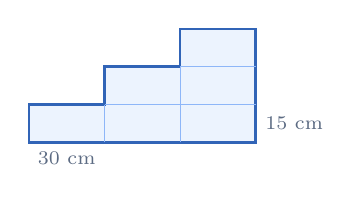
\begin{tikzpicture}[scale=0.032]
\draw[geo,fill=tmBlue!10] (0,0)--(90,0)--(90,45)--(60,45)--(60,30)--(30,30)--(30,15)--(0,15)--cycle;
\draw[tmBlue!60,line width=0.35pt] (30,0)--(30,15) (60,0)--(60,30) (30,15)--(90,15) (60,30)--(90,30);
\node[dim,below] at (15,0){$30$ cm}; \node[dim,right] at (90,7.5){$15$ cm};
\end{tikzpicture}
\end{minipage}
\end{probbox}
\probsol{
Cut the steps into three layers, each $15$ cm $=0.15$ m high:\par
bottom layer $0.9$ m deep, middle layer $0.6$ m deep, top layer $0.3$ m deep.\par
Volume: $1.5\times0.15\times(0.9+0.6+0.3)=1.5\times0.15\times1.8=0.405$ m$^3$.
\dapso{$0.405$ m$^3$.}}
\gap
\begin{probbox}{50}{\stars{2}}
A tank is $1.5$ m long. The water in it is $60$ cm deep. After $240$ l of water are added, it is $80$ cm deep. Find the width of the tank.
\end{probbox}
\probsol{
$240$ l $=240$ dm$^3$; the rise is $80-60=20$ cm $=2$ dm.\par
Base area: $240:2=120$ dm$^2=1.2$ m$^2$.\par
Width: $1.2:1.5=0.8$ m.
\dapso{$0.8$ m.}}
\clearpage
\titlehead
\begingroup\setbox0=\vbox{\section*{Cube Stacks and Painted Faces}}\endgroup
\chapterhead{5}{Cube Stacks and Painted Faces}
\tikzset{xhf/.style={draw=tmBlue!70!black,line width=0.45pt,line join=round}}
\providecommand{\xhcuboid}{}\renewcommand{\xhcuboid}[7][tmBlue]{\begin{scope}[shift={({#2+0.5*(#3)},{#4+0.35*(#3)})}]
\filldraw[xhf,fill=#1!22] (0,0) rectangle (#5,#7);
\filldraw[xhf,fill=#1!8] (0,#7)--(#5,#7)--({#5+0.5*(#6)},{#7+0.35*(#6)})--({0.5*(#6)},{#7+0.35*(#6)})--cycle;
\filldraw[xhf,fill=#1!45] (#5,0)--({#5+0.5*(#6)},{0.35*(#6)})--({#5+0.5*(#6)},{#7+0.35*(#6)})--(#5,#7)--cycle;
\end{scope}}
\providecommand{\xhcube}{}\renewcommand{\xhcube}[4][tmBlue]{\xhcuboid[#1]{#2}{#3}{#4}{1}{1}{1}}

\shead{Building a box from small blocks}
\begin{knowbox}
\begin{minipage}[t]{0.62\linewidth}
When equal small blocks (unit cubes, small cubes, bricks) are stacked tightly into a new solid, the \textbf{volume of the new solid} is the sum of the volumes of the blocks:
\[V_{\text{big}}=V_{\text{one block}}\times\text{number of blocks}.\]
To find the lateral area, total surface area or volume of a box built from equal blocks:\par
\smallskip
\textbf{Step 1.} Find the dimensions of the big box:\par
length $=$ length of a block $\times$ number of blocks along the length;\par
width $=$ width of a block $\times$ number of blocks along the width;\par
height $=$ height of a block $\times$ number of layers.\par
\smallskip
\textbf{Step 2.} Use the formulas for the cuboid or cube.
\end{minipage}\hfill
\begin{minipage}[t]{0.34\linewidth}\vspace{4pt}\centering
\begin{tikzpicture}[scale=0.62]
\xhcube{0}{1}{0}\xhcube{1}{1}{0}\xhcube{2}{1}{0}\xhcube{0}{1}{1}\xhcube{1}{1}{1}\xhcube{2}{1}{1}\xhcube{0}{0}{0}\xhcube{1}{0}{0}\xhcube{2}{0}{0}\xhcube{0}{0}{1}\xhcube{1}{0}{1}\xhcube{2}{0}{1}
\node[dim,below] at (1.5,0){$3$ cubes};
\node[dim,right] at (4,0.6){$2$ layers};
\end{tikzpicture}\par\smallskip
{\small $3\times2\times2=12$ cubes}
\end{minipage}
\end{knowbox}

\shead{How many cubes fit in a box?}
\begin{knowbox}
To pack cubes of edge $a$ into a box (all lengths in the same unit):\par
\smallskip
-- along each edge of the box, count how many times $a$ fits (the quotient; any remainder is wasted space);\par
-- number of cubes $=$ (number along the length) $\times$ (number along the width) $\times$ (number along the height).\par
\smallskip
If a big cube is built from small cubes, the edge of the big cube is a whole number of small edges, so
\[\text{number of small cubes}=n\times n\times n,\qquad n=\text{big edge}:\text{small edge}.\]
If we know the total surface area of the big cube, one face is $S_{\text{total}}:6$, and the edge is the number that multiplied by itself gives this area.
\end{knowbox}

\shead{Painting the outside of a solid made of small cubes}
\begin{knowbox}
\begin{minipage}[t]{0.6\linewidth}
A big cube with $n$ small cubes along each edge ($n\ge3$) is painted on all $6$ faces, then taken apart:\par
\smallskip
-- \textbf{painted on $3$ faces}: the cubes at the $8$ corners: $8$ cubes;\par
-- \textbf{painted on exactly $2$ faces}: on the $12$ edges, not at corners: $12\times(n-2)$;\par
-- \textbf{painted on exactly $1$ face}: on the $6$ faces, not on edges: $6\times(n-2)\times(n-2)$;\par
-- \textbf{not painted}: the hidden core, a cube of edge $n-2$: $(n-2)\times(n-2)\times(n-2)$.\par
\smallskip
For a box with $a,\ b,\ c$ small cubes along its edges (all $\ge3$): $3$ faces: $8$; exactly $2$ faces: $4\times[(a-2)+(b-2)+(c-2)]$; exactly $1$ face: $2\times[(a-2)(b-2)+(b-2)(c-2)+(a-2)(c-2)]$; none: $(a-2)(b-2)(c-2)$.
\end{minipage}\hfill
\begin{minipage}[t]{0.37\linewidth}\vspace{4pt}\centering
\begin{tikzpicture}[scale=0.5]
\xhcube[tmOrange]{0}{3}{0}\xhcube[tmGreen]{1}{3}{0}\xhcube[tmGreen]{2}{3}{0}\xhcube[tmOrange]{3}{3}{0}\xhcube[tmGreen]{0}{3}{1}\xhcube[tmBlue]{1}{3}{1}\xhcube[tmBlue]{2}{3}{1}\xhcube[tmGreen]{3}{3}{1}\xhcube[tmGreen]{0}{3}{2}\xhcube[tmBlue]{1}{3}{2}\xhcube[tmBlue]{2}{3}{2}\xhcube[tmGreen]{3}{3}{2}\xhcube[tmOrange]{0}{3}{3}\xhcube[tmGreen]{1}{3}{3}\xhcube[tmGreen]{2}{3}{3}\xhcube[tmOrange]{3}{3}{3}\xhcube[tmGreen]{0}{2}{0}\xhcube[tmBlue]{1}{2}{0}\xhcube[tmBlue]{2}{2}{0}\xhcube[tmGreen]{3}{2}{0}\xhcube[tmBlue]{0}{2}{1}\xhcube[tmBlue]{3}{2}{1}\xhcube[tmBlue]{0}{2}{2}\xhcube[tmBlue]{3}{2}{2}\xhcube[tmGreen]{0}{2}{3}\xhcube[tmBlue]{1}{2}{3}\xhcube[tmBlue]{2}{2}{3}\xhcube[tmGreen]{3}{2}{3}\xhcube[tmGreen]{0}{1}{0}\xhcube[tmBlue]{1}{1}{0}\xhcube[tmBlue]{2}{1}{0}\xhcube[tmGreen]{3}{1}{0}\xhcube[tmBlue]{0}{1}{1}\xhcube[tmBlue]{3}{1}{1}\xhcube[tmBlue]{0}{1}{2}\xhcube[tmBlue]{3}{1}{2}\xhcube[tmGreen]{0}{1}{3}\xhcube[tmBlue]{1}{1}{3}\xhcube[tmBlue]{2}{1}{3}\xhcube[tmGreen]{3}{1}{3}\xhcube[tmOrange]{0}{0}{0}\xhcube[tmGreen]{1}{0}{0}\xhcube[tmGreen]{2}{0}{0}\xhcube[tmOrange]{3}{0}{0}\xhcube[tmGreen]{0}{0}{1}\xhcube[tmBlue]{1}{0}{1}\xhcube[tmBlue]{2}{0}{1}\xhcube[tmGreen]{3}{0}{1}\xhcube[tmGreen]{0}{0}{2}\xhcube[tmBlue]{1}{0}{2}\xhcube[tmBlue]{2}{0}{2}\xhcube[tmGreen]{3}{0}{2}\xhcube[tmOrange]{0}{0}{3}\xhcube[tmGreen]{1}{0}{3}\xhcube[tmGreen]{2}{0}{3}\xhcube[tmOrange]{3}{0}{3}
\end{tikzpicture}\par\smallskip
{\scriptsize\textcolor{tmOrange}{\rule{6pt}{6pt}}\,$3$ faces\quad\textcolor{tmGreen}{\rule{6pt}{6pt}}\,$2$ faces\quad\textcolor{tmBlue}{\rule{6pt}{6pt}}\,$1$ face}
\end{minipage}\par
\smallskip
\emph{Check:} the four groups add up to all the small cubes. If an edge has fewer than $3$ small cubes, count directly.
\end{knowbox}

\shead{Counting cubes in a stack. Views}
\begin{knowbox}
\begin{minipage}[t]{0.6\linewidth}
To count the cubes in a stack, count \textbf{column by column} (or layer by layer). Unless the problem says otherwise, every cube rests on the table or on another cube, so hidden cubes are under the visible ones.\par
\smallskip
A \textbf{top view with numbers} shows the base squares; the number in each square is how many cubes are stacked there. The number of cubes is the sum of these numbers.\par
\smallskip
In the \textbf{front view}, each column is as tall as the tallest stack in that column.
\end{minipage}\hfill
\begin{minipage}[t]{0.36\linewidth}\vspace{2pt}\centering
\begin{tikzpicture}[scale=0.5]
\foreach \x/\y/\h in {0/1/2,1/1/3,2/1/1,0/0/1,1/0/2,2/0/1}{\draw[xhf,fill=tmBlue!8] (\x,\y) rectangle ++(1,1); \node[font=\small\bfseries] at (\x+0.5,\y+0.5){\h};}
\node[dim,below] at (1.5,0){front};
\node[dim,above] at (1.5,2){top view};
\end{tikzpicture}\par\smallskip
$2+3+1+1+2+1=10$ cubes
\end{minipage}
\end{knowbox}
\gap
\begin{exbox}{\ExWord\ 1}
\begin{minipage}[t]{0.6\linewidth}
A brick is a cuboid $24$ cm long, $12$ cm wide and $6$ cm high. A builder stacks $6$ such bricks into a block shaped like a cuboid: $2$ bricks side by side in each layer, $3$ layers (see the figure).\par
\pa{a} Find the lateral area and the total surface area of the block.\par
\pa{b} Find the volume of the block.
\end{minipage}\hfill
\begin{minipage}[t]{0.36\linewidth}\vspace{0pt}\centering
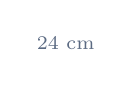
\begin{tikzpicture}[scale=0.085]
\xhcuboid[tmOrange]{0}{12}{0}{24}{12}{6}\xhcuboid[tmOrange]{0}{12}{6}{24}{12}{6}\xhcuboid[tmOrange]{0}{12}{12}{24}{12}{6}
\xhcuboid[tmOrange]{0}{0}{0}{24}{12}{6}\xhcuboid[tmOrange]{0}{0}{6}{24}{12}{6}\xhcuboid[tmOrange]{0}{0}{12}{24}{12}{6}
\node[dim,below] at (12,0){$24$ cm};
\end{tikzpicture}
\end{minipage}
\guide
\pa{a} Length of the block: $24$ cm.\par
Width of the block: $12\times2=24$ cm.\par
Height of the block: $6\times3=18$ cm.\par
Lateral area: $(24+24)\times2\times18=1\,728$ cm$^2$.\par
Area of the base: $24\times24=576$ cm$^2$.\par
Total surface area: $1\,728+576\times2=2\,880$ cm$^2$.\par
\pa{b} \emph{Method 1.} $V=24\times24\times18=10\,368$ cm$^3$.\par
\emph{Method 2.} One brick: $24\times12\times6=1\,728$ cm$^3$; $6$ bricks: $1\,728\times6=10\,368$ cm$^3$.
\dapso{\pa{a} $1\,728$ cm$^2$; $2\,880$ cm$^2$;\par \pa{b} $10\,368$ cm$^3$.}
\end{exbox}
\gap
\begin{exbox}{\ExWord\ 2}
Small cubes of edge $2$ cm are stacked into a big cube whose total surface area is $864$ cm$^2$. How many small cubes are used?
\guide
\emph{Method 1.} One face of the big cube: $864:6=144$ cm$^2$.\par
$144=12\times12$, so the edge of the big cube is $12$ cm.\par
Along each edge there are $12:2=6$ small cubes.\par
Number of small cubes: $6\times6\times6=216$.\par
\emph{Method 2.} The edge of the big cube is $12$ cm (as above).\par
Volume of the big cube: $12\times12\times12=1\,728$ cm$^3$.\par
Volume of a small cube: $2\times2\times2=8$ cm$^3$.\par
Number of small cubes: $1\,728:8=216$.
\dapso{$216$ small cubes.}
\end{exbox}
\gap
\begin{exbox}{\ExWord\ 3}
A crate (a cuboid) is $1.2$ m long, $0.8$ m wide and $0.5$ m high.\par
\pa{a} At most how many cube-shaped toy blocks of edge $1$ dm fit in the crate?\par
\pa{b} At most how many cube-shaped gift boxes of edge $3$ dm fit in the crate?
\guide
Change units: $1.2$ m $=12$ dm; $0.8$ m $=8$ dm; $0.5$ m $=5$ dm.\par
\pa{a} Along the length: $12:1=12$ blocks; along the width: $8$ blocks; along the height: $5$ blocks.\par
Number of blocks: $12\times8\times5=480$.\par
\pa{b} Along the length: $12:3=4$ boxes.\par
Along the width: $8:3=2$ (remainder $2$ dm), so $2$ boxes.\par
Along the height: $5:3=1$ (remainder $2$ dm), so $1$ box.\par
Number of gift boxes: $4\times2\times1=8$.
\dapso{\pa{a} $480$ blocks;\par \pa{b} $8$ boxes.}
\end{exbox}
\gap
\begin{exbox}{\ExWord\ 4}
Mai glues $1$ cm cubes into a big cube of edge $5$ cm and paints all $6$ outside faces.\par
\pa{a} How many small cubes did she use?\par
\pa{b} How many small cubes are painted on $3$ faces? On exactly $2$ faces? On exactly $1$ face? On no face?
\guide
\pa{a} Each edge has $5:1=5$ small cubes.\par Number of small cubes: $5\times5\times5=125$.\par
\pa{b} Painted on $3$ faces: the $8$ corner cubes.\par
Each edge has $5-2=3$ cubes that are not corners.\par
Exactly $2$ faces: $12\times3=36$.\par
Each face has $3\times3=9$ cubes not on an edge.\par
Exactly $1$ face: $6\times9=54$.\par
No face: the core cube of edge $3$: $3\times3\times3=27$.\par
\emph{Check:} $8+36+54+27=125$.
\dapso{\pa{a} $125$;\par \pa{b} $8$; $36$; $54$; $27$.}
\end{exbox}
\gap
\begin{exbox}{\ExWord\ 5}
\begin{minipage}[t]{0.58\linewidth}
Nam builds the stack of cubes in the figure.\par
\pa{a} How many cubes are in the stack?\par
\pa{b} Draw the front view.\par
\pa{c} How many more cubes does Nam need to turn the stack into a cuboid $3$ cubes long, $2$ cubes wide and $3$ cubes high?
\end{minipage}\hfill
\begin{minipage}[t]{0.38\linewidth}\vspace{0pt}\centering

\begin{tikzpicture}[scale=0.5]
\xhcube{0}{1}{0}\xhcube{1}{1}{0}\xhcube{2}{1}{0}\xhcube{0}{1}{1}\xhcube{1}{1}{1}\xhcube{1}{1}{2}\xhcube{0}{0}{0}\xhcube{1}{0}{0}\xhcube{2}{0}{0}\xhcube{1}{0}{1}
\node[dim,below] at (1.5,0){front};
\end{tikzpicture}
\end{minipage}
\guide
\pa{a} Write the number of cubes on each base square (top view):\par
\begin{center}\begin{tikzpicture}[scale=0.45]
\foreach \x/\y/\h in {0/1/2,1/1/3,2/1/1,0/0/1,1/0/2,2/0/1}{\draw[xhf,fill=tmBlue!8] (\x,\y) rectangle ++(1,1); \node[font=\small\bfseries] at (\x+0.5,\y+0.5){\h};}
\node[dim,below] at (1.5,0){front};
\end{tikzpicture}\qquad
\begin{tikzpicture}[scale=0.45]
\foreach \x/\y in {0/0,0/1,1/0,1/1,1/2,2/0}{\draw[xhf,fill=tmBlue!20] (\x,\y) rectangle ++(1,1);}
\node[dim,below] at (1.5,0){front view};
\end{tikzpicture}\end{center}
Back row: $2+3+1=6$ cubes; front row: $1+2+1=4$ cubes.\par
Number of cubes: $6+4=10$.\par
\pa{b} The columns of the front view are as tall as the tallest stacks: $2$, $3$, $1$ (figure above).\par
\pa{c} The cuboid has $3\times2\times3=18$ cubes.\par
Cubes still needed: $18-10=8$.
\dapso{\pa{a} $10$ cubes;\par \pa{c} $8$ cubes.}
\end{exbox}
\dividerbar{Practice}
\begin{probbox}{1}{\relax}
How many $1$ cm cubes are needed to build a cube of edge $6$ cm?
\end{probbox}
\probsol{
Each edge has $6:1=6$ small cubes.\par
Number of small cubes: $6\times6\times6=216$.
\dapso{$216$ cubes.}}
\gap
\begin{probbox}{2}{\relax}
How many cubes of edge $3$ cm are needed to build a cube of edge $12$ cm?
\end{probbox}
\probsol{
Each edge has $12:3=4$ small cubes.\par
Number of small cubes: $4\times4\times4=64$.
\dapso{$64$ cubes.}}
\gap
\begin{probbox}{3}{\relax}
How many cubes of edge $2$ cm are needed to fill a box $10$ cm long, $8$ cm wide and $6$ cm high?
\end{probbox}
\probsol{
Along the length: $10:2=5$; along the width: $8:2=4$; along the height: $6:2=3$.\par
Number of cubes: $5\times4\times3=60$.
\dapso{$60$ cubes.}}
\gap
\begin{probbox}{4}{\relax}
A toy chest is $1.2$ m long, $0.6$ m wide and $0.4$ m high. How many cube-shaped blocks of edge $2$ dm fill it exactly?
\end{probbox}
\probsol{
$1.2$ m $=12$ dm; $0.6$ m $=6$ dm; $0.4$ m $=4$ dm.\par
Along the length: $12:2=6$; along the width: $6:2=3$; along the height: $4:2=2$.\par
Number of blocks: $6\times3\times2=36$.
\dapso{$36$ blocks.}}
\gap
\begin{probbox}{5}{\relax}
$64$ small cubes, each with volume $1$ cm$^3$, are stacked into a big cube. Find the lateral area, the total surface area and the volume of the big cube.
\end{probbox}
\probsol{
A small cube of volume $1$ cm$^3$ has edge $1$ cm.\par
$64=4\times4\times4$, so each edge of the big cube has $4$ small cubes: the edge is $4$ cm.\par
Lateral area: $4\times4\times4=64$ cm$^2$.\par
Total surface area: $4\times4\times6=96$ cm$^2$.\par
Volume: $64\times1=64$ cm$^3$.
\dapso{$64$ cm$^2$; $96$ cm$^2$; $64$ cm$^3$.}}
\gap
\begin{probbox}{6}{\relax}
$125$ small cubes, each with volume $27$ cm$^3$, are stacked into a big cube. Find the total surface area and the volume of the big cube.
\end{probbox}
\probsol{
$27=3\times3\times3$, so a small cube has edge $3$ cm.\par
$125=5\times5\times5$, so the big cube has $5$ small cubes along each edge.\par
Edge of the big cube: $3\times5=15$ cm.\par
Total surface area: $15\times15\times6=1\,350$ cm$^2$.\par
Volume: $27\times125=3\,375$ cm$^3$.
\dapso{$1\,350$ cm$^2$; $3\,375$ cm$^3$.}}
\gap
\begin{probbox}{7}{\relax}
A big cube with total surface area $216$ cm$^2$ is built from $1$ cm cubes. How many small cubes are used?
\end{probbox}
\probsol{
One face: $216:6=36$ cm$^2$.\par
$36=6\times6$, so the edge is $6$ cm.\par
Number of small cubes: $6\times6\times6=216$.
\dapso{$216$ cubes.}}
\gap
\begin{probbox}{8}{\relax}
A big cube with lateral area $400$ cm$^2$ is built from cubes of edge $2$ cm. How many small cubes are used?
\end{probbox}
\probsol{
One face: $400:4=100$ cm$^2$.\par
$100=10\times10$, so the edge is $10$ cm.\par
Along each edge: $10:2=5$ small cubes.\par
Number of small cubes: $5\times5\times5=125$.
\dapso{$125$ cubes.}}
\gap
\begin{probbox}{9}{\relax}
Five bricks, each $20$ cm long, $10$ cm wide and $5$ cm high, are laid flat one on top of another. Find the lateral area, the total surface area and the volume of the pile.
\end{probbox}
\probsol{
The pile is a cuboid $20$ cm long, $10$ cm wide and $5\times5=25$ cm high.\par
Lateral area: $(20+10)\times2\times25=1\,500$ cm$^2$.\par
Total surface area: $1\,500+20\times10\times2=1\,900$ cm$^2$.\par
Volume: $20\times10\times25=5\,000$ cm$^3$.
\dapso{$1\,500$ cm$^2$; $1\,900$ cm$^2$; $5\,000$ cm$^3$.}}
\gap
\begin{probbox}{10}{\relax}
Two equal cubes are stacked to make a cuboid $16$ cm high. Find the lateral area and the total surface area of the cuboid.
\end{probbox}
\probsol{
Edge of each cube: $16:2=8$ cm.\par
The cuboid is $8$ cm long, $8$ cm wide and $16$ cm high.\par
Lateral area: $(8+8)\times2\times16=512$ cm$^2$.\par
Total surface area: $512+8\times8\times2=640$ cm$^2$.
\dapso{$512$ cm$^2$; $640$ cm$^2$.}}
\gap
\begin{probbox}{11}{\relax}
Three equal cubes are put in a row to make a cuboid $21$ cm long. Find the total surface area of the cuboid.
\end{probbox}
\probsol{
Edge of each cube: $21:3=7$ cm. One face: $7\times7=49$ cm$^2$.\par
The four long sides of the cuboid consist of $3\times4=12$ cube faces; the two ends are $2$ more faces.\par
Total surface area: $49\times14=686$ cm$^2$.\par
\emph{Check:} $2\times(21\times7+21\times7+7\times7)=686$ cm$^2$.
\dapso{$686$ cm$^2$.}}
\gap
\begin{probbox}{12}{\relax}
A carton is $60$ cm long, $40$ cm wide and $30$ cm high. How many cube-shaped boxes of edge $10$ cm fill it exactly?
\end{probbox}
\probsol{
Along the length: $60:10=6$; along the width: $40:10=4$; along the height: $30:10=3$.\par
Number of boxes: $6\times4\times3=72$.
\dapso{$72$ boxes.}}
\gap
\begin{probbox}{13}{\relax}
A drawer is $50$ cm long, $35$ cm wide and $22$ cm high. At most how many cube-shaped boxes of edge $10$ cm fit in it?
\end{probbox}
\probsol{
Along the length: $50:10=5$.\par
Along the width: $35:10=3$ (remainder $5$ cm), so $3$ boxes.\par
Along the height: $22:10=2$ (remainder $2$ cm), so $2$ boxes.\par
Number of boxes: $5\times3\times2=30$.
\dapso{$30$ boxes.}}
\gap
\begin{probbox}{14}{\relax}
A crate is $9$ dm long, $6$ dm wide and $4$ dm high. Cube-shaped boxes of edge $3$ dm are packed in it.\par
\pa{a} At most how many boxes fit?\par
\pa{b} With that many boxes inside, how much space in the crate is left empty?
\end{probbox}
\probsol{
\pa{a} Along the length: $9:3=3$; along the width: $6:3=2$; along the height: $4:3=1$ (remainder $1$ dm).\par
Number of boxes: $3\times2\times1=6$.\par
\pa{b} Volume of the crate: $9\times6\times4=216$ dm$^3$.\par
Volume of $6$ boxes: $3\times3\times3\times6=162$ dm$^3$.\par
Empty space: $216-162=54$ dm$^3$.
\dapso{\pa{a} $6$ boxes;\par \pa{b} $54$ dm$^3$.}}
\gap
\begin{probbox}{15}{\relax}
A cube of edge $3$ cm made of $1$ cm cubes is painted on all its faces. How many small cubes are painted on $3$ faces, on exactly $2$ faces, on exactly $1$ face, on no face?
\end{probbox}
\probsol{
Each edge has $3$ small cubes; $3-2=1$ of them is not a corner.\par
$3$ faces: $8$.\par
Exactly $2$ faces: $12\times1=12$.\par
Exactly $1$ face: $6\times1\times1=6$.\par
No face: $1\times1\times1=1$ (the cube in the very middle).\par
\emph{Check:} $8+12+6+1=27=3\times3\times3$.
\dapso{$8$; $12$; $6$; $1$.}}
\gap
\begin{probbox}{16}{\relax}
A big cube is made of $216$ equal small cubes and then painted on all its faces. How many small cubes are painted on exactly $2$ faces? On exactly $1$ face?
\end{probbox}
\probsol{
$216=6\times6\times6$, so each edge has $6$ small cubes.\par
Exactly $2$ faces: $12\times(6-2)=48$.\par
Exactly $1$ face: $6\times4\times4=96$.
\dapso{$48$; $96$.}}
\gap
\begin{probbox}{17}{\relax}
A big cube is made of $343$ equal small cubes and then painted on all its faces. How many small cubes have no paint at all?
\end{probbox}
\probsol{
$343=7\times7\times7$, so each edge has $7$ small cubes.\par
The unpainted cubes form a core cube with $7-2=5$ cubes along each edge.\par
Number of unpainted cubes: $5\times5\times5=125$.
\dapso{$125$ cubes.}}
\gap
\begin{probbox}{18}{\relax}
A cube of edge $10$ cm is built from $1$ cm cubes and painted on all its faces. How many small cubes are painted on at least $2$ faces?
\end{probbox}
\probsol{
Each edge has $10$ small cubes.\par
Painted on $3$ faces: $8$.\par
Painted on exactly $2$ faces: $12\times(10-2)=96$.\par
At least $2$ faces: $8+96=104$.
\dapso{$104$ cubes.}}
\gap
\begin{probbox}{19}{\relax}
A cuboid $5$ cm long, $4$ cm wide and $3$ cm high is built from $1$ cm cubes and painted on all its faces. How many small cubes are painted on $3$ faces, on exactly $2$ faces, on exactly $1$ face, on no face?
\end{probbox}
\probsol{
Along the edges there are $5$, $4$, $3$ cubes; without the corners: $3$, $2$, $1$.\par
$3$ faces: $8$.\par
Exactly $2$ faces: $4\times(3+2+1)=24$.\par
Exactly $1$ face: $2\times(3\times2+2\times1+3\times1)=22$.\par
No face: $3\times2\times1=6$.\par
\emph{Check:} $8+24+22+6=60=5\times4\times3$.
\dapso{$8$; $24$; $22$; $6$.}}
\gap
\begin{probbox}{20}{\relax}
A cuboid $14$ cm long, $10$ cm wide and $6$ cm high is built from cubes of edge $2$ cm and painted on all its faces. How many small cubes are painted on exactly $2$ faces, on exactly $1$ face, on no face?
\end{probbox}
\probsol{
Along the edges: $14:2=7$, $10:2=5$, $6:2=3$ cubes; without the corners: $5$, $3$, $1$.\par
Exactly $2$ faces: $4\times(5+3+1)=36$.\par
Exactly $1$ face: $2\times(5\times3+3\times1+5\times1)=46$.\par
No face: $5\times3\times1=15$.
\dapso{$36$; $46$; $15$.}}
\gap
\begin{probbox}{21}{\relax}
A big cube made of equal small cubes is painted on all its faces. Exactly $64$ small cubes have no paint. How many small cubes are there in all, and how many are painted on exactly $1$ face?
\end{probbox}
\probsol{
The unpainted core is a cube: $64=4\times4\times4$, so it has $4$ cubes along each edge.\par
The big cube has $4+2=6$ cubes along each edge.\par
In all: $6\times6\times6=216$ small cubes.\par
Exactly $1$ face: $6\times4\times4=96$.
\dapso{$216$ cubes; $96$ cubes.}}
\gap
\begin{probbox}{22}{\relax}
A big cube made of equal small cubes is painted on all its faces. Exactly $150$ small cubes are painted on just $1$ face. How many small cubes are there in all?
\end{probbox}
\probsol{
On each face: $150:6=25$ such cubes; $25=5\times5$.\par
So $n-2=5$, and each edge has $7$ small cubes.\par
In all: $7\times7\times7=343$.
\dapso{$343$ cubes.}}
\gap
\begin{probbox}{23}{\relax}
A big cube is built from $1$ cm cubes and painted on all its faces. Exactly $84$ small cubes are painted on $2$ faces. Find the volume of the big cube.
\end{probbox}
\probsol{
On each edge: $84:12=7$ such cubes.\par
Each edge has $7+2=9$ small cubes, so the edge is $9$ cm.\par
Volume: $9\times9\times9=729$ cm$^3$.
\dapso{$729$ cm$^3$.}}
\gap
\begin{probbox}{24}{\relax}
A cube of edge $5$ cm is built from $1$ cm cubes. The top layer is then lifted off. How many small cubes are left, and what is the total surface area of the remaining solid?
\end{probbox}
\probsol{
One layer has $5\times5=25$ cubes, so $125-25=100$ cubes are left.\par
The remaining solid is a cuboid $5$ cm long, $5$ cm wide and $4$ cm high.\par
Lateral area: $(5+5)\times2\times4=80$ cm$^2$.\par
Total surface area: $80+5\times5\times2=130$ cm$^2$.
\dapso{$100$ cubes; $130$ cm$^2$.}}
\gap
\begin{probbox}{25}{\relax}
A cube of edge $4$ cm is built from $1$ cm cubes. One corner cube is removed. Find the total surface area of the remaining solid.
\end{probbox}
\probsol{
Total surface area at first: $4\times4\times6=96$ cm$^2$.\par
Removing the corner cube takes away $3$ outside squares of $1$ cm$^2$, but uncovers $3$ new squares of $1$ cm$^2$ inside the gap.\par
The area does not change: $96-3+3=96$ cm$^2$.
\dapso{$96$ cm$^2$.}}
\gap
\begin{probbox}{26}{\relax}
\begin{minipage}[t]{0.6\linewidth}
How many cubes are there in this staircase? (No cube is missing from the back.)
\end{minipage}\hfill
\begin{minipage}[t]{0.36\linewidth}\vspace{0pt}\centering
\begin{tikzpicture}[scale=0.45]
\xhcube{0}{1}{0}\xhcube{1}{1}{0}\xhcube{2}{1}{0}\xhcube{1}{1}{1}\xhcube{2}{1}{1}\xhcube{2}{1}{2}\xhcube{0}{0}{0}\xhcube{1}{0}{0}\xhcube{2}{0}{0}\xhcube{1}{0}{1}\xhcube{2}{0}{1}\xhcube{2}{0}{2}
\end{tikzpicture}
\end{minipage}
\end{probbox}
\probsol{
The staircase is $2$ cubes deep.\par
Seen from the front, the columns have $1$, $2$ and $3$ cubes: $1+2+3=6$ cubes in one row.\par
Number of cubes: $6\times2=12$.
\dapso{$12$ cubes.}}
\gap
\begin{probbox}{27}{\relax}
\begin{minipage}[t]{0.6\linewidth}
The figure is the top view of a stack of cubes; each number tells how many cubes stand on that square.\par
\pa{a} How many cubes are in the stack?\par
\pa{b} How tall is each column of the front view?
\end{minipage}\hfill
\begin{minipage}[t]{0.36\linewidth}\vspace{0pt}\centering
\begin{tikzpicture}[scale=0.5]
\foreach \x/\y/\h in {0/1/3,1/1/1,2/1/2,0/0/2,1/0/2,2/0/1}{\draw[xhf,fill=tmBlue!8] (\x,\y) rectangle ++(1,1); \node[font=\small\bfseries] at (\x+0.5,\y+0.5){\h};}
\node[dim,below] at (1.5,0){front};
\end{tikzpicture}
\end{minipage}
\end{probbox}
\probsol{
\pa{a} $3+1+2+2+2+1=11$ cubes.\par
\pa{b} From left to right, the tallest stack in each column has $3$, $2$ and $2$ cubes.
\dapso{\pa{a} $11$ cubes;\par \pa{b} $3$, $2$, $2$.}}
\gap
\begin{probbox}{28}{\relax}
\begin{minipage}[t]{0.6\linewidth}
How many cubes are in the stack? How many more cubes are needed to have enough for a cube with $3$ small cubes along each edge?
\end{minipage}\hfill
\begin{minipage}[t]{0.36\linewidth}\vspace{0pt}\centering
\begin{tikzpicture}[scale=0.45]
\xhcube{0}{1}{0}\xhcube{1}{1}{0}\xhcube{2}{1}{0}\xhcube{0}{1}{1}\xhcube{1}{1}{1}\xhcube{2}{1}{1}\xhcube{0}{1}{2}\xhcube{1}{1}{2}\xhcube{2}{1}{2}\xhcube{0}{0}{0}\xhcube{1}{0}{0}\xhcube{2}{0}{0}\xhcube{0}{0}{1}\xhcube{1}{0}{1}\xhcube{2}{0}{1}
\end{tikzpicture}
\end{minipage}
\end{probbox}
\probsol{
Front row: $3\times2=6$ cubes; back row: $3\times3=9$ cubes.\par
Number of cubes: $6+9=15$.\par
A cube with $3$ small cubes along each edge has $3\times3\times3=27$ cubes.\par
More cubes needed: $27-15=12$.
\dapso{$15$ cubes; $12$ more cubes.}}
\gap
\begin{probbox}{29}{\relax}
Khoa stacks $64$ dice, each a cube of edge $2$ cm, into one big cube. Find the total surface area and the volume of the big cube.
\end{probbox}
\probsol{
$64=4\times4\times4$, so each edge has $4$ dice.\par
Edge of the big cube: $2\times4=8$ cm.\par
Total surface area: $8\times8\times6=384$ cm$^2$.\par
Volume: $8\times8\times8=512$ cm$^3$.
\dapso{$384$ cm$^2$; $512$ cm$^3$.}}
\gap
\begin{probbox}{30}{\relax}
A wooden block $12$ dm long, $8$ dm wide and $6$ dm high is painted on all its faces and then sawn into cubes of edge $2$ dm. How many cubes are there? How many have no paint? How many are painted on exactly $1$ face?
\end{probbox}
\probsol{
Along the edges: $12:2=6$, $8:2=4$, $6:2=3$ cubes.\par
Number of cubes: $6\times4\times3=72$.\par
Without the corners: $4$, $2$, $1$ cubes along the edges.\par
No paint: $4\times2\times1=8$.\par
Exactly $1$ face: $2\times(4\times2+2\times1+4\times1)=28$.
\dapso{$72$ cubes; $8$ cubes; $28$ cubes.}}
\dividerbar{Challenge -- Extension}
\begin{probbox}{31}{\stars{1}}
A big cube made of small cubes is painted on all its faces. The number of small cubes painted on exactly $1$ face equals the number painted on exactly $2$ faces. How many small cubes make up the big cube?
\end{probbox}
\probsol{
Let each edge have $n$ small cubes and put $k=n-2$.\par
Exactly $1$ face: $6\times k\times k$; exactly $2$ faces: $12\times k$.\par
$6\times k\times k=12\times k$ gives $k=2$, so $n=4$.\par
Number of small cubes: $4\times4\times4=64$.
\dapso{$64$ cubes.}}
\gap
\begin{probbox}{32}{\stars{2}}
A big cube made of small cubes is painted on all its faces. The number of unpainted small cubes equals the number of small cubes painted on exactly $1$ face. How many small cubes are there?
\end{probbox}
\probsol{
Let $k=n-2$. Unpainted: $k\times k\times k$; exactly $1$ face: $6\times k\times k$.\par
$k\times k\times k=6\times k\times k$ gives $k=6$, so $n=8$.\par
Number of small cubes: $8\times8\times8=512$.\par
\emph{Check:} unpainted $6\times6\times6=216$; one face $6\times36=216$.
\dapso{$512$ cubes.}}
\gap
\begin{probbox}{33}{\stars{1}}
A cube of edge $4$ cm made of $1$ cm cubes is painted on all its faces and taken apart. What fraction of all the faces of the small cubes is painted?
\end{probbox}
\probsol{
Painted squares: the surface of the big cube, $4\times4\times6=96$ squares.\par
All faces of the small cubes: $64\times6=384$ squares.\par
Fraction painted: $\dfrac{96}{384}=\dfrac14$.
\dapso{$\dfrac14$.}}
\gap
\begin{probbox}{34}{\stars{1}}
A cube of edge $5$ cm is built from $1$ cm cubes. Only its $4$ side faces are painted (not the top, not the bottom). How many small cubes are painted on exactly $2$ faces, on exactly $1$ face, on no face?
\end{probbox}
\probsol{
Each of the $5$ layers is a $5\times5$ square whose border is painted.\par
In one layer: $4$ corner cubes with $2$ faces; $4\times3=12$ cubes with $1$ face; $3\times3=9$ unpainted.\par
Exactly $2$ faces: $4\times5=20$.\par
Exactly $1$ face: $12\times5=60$.\par
No face: $9\times5=45$.\par
\emph{Check:} $20+60+45=125$.
\dapso{$20$; $60$; $45$.}}
\gap
\begin{probbox}{35}{\stars{2}}
A cube of edge $6$ cm is built from $1$ cm cubes. The $4$ side faces are painted blue; the top and the bottom are painted red. How many small cubes carry both colours?
\end{probbox}
\probsol{
A cube with red paint lies in the top layer or the bottom layer.\par
It also has blue paint if it lies on the border of that layer.\par
Border of a $6\times6$ layer: $6\times6-4\times4=20$ cubes.\par
Both colours: $20\times2=40$ cubes.
\dapso{$40$ cubes.}}
\gap
\begin{probbox}{36}{\stars{1}}
$343$ cubes of edge $2$ cm are stacked into a big cube. The top layer is then lifted off. Find the total surface area of the remaining solid.
\end{probbox}
\probsol{
$343=7\times7\times7$, so the big cube is $2\times7=14$ cm along each edge.\par
Without the top layer it is a cuboid $14$ cm by $14$ cm by $14-2=12$ cm.\par
Lateral area: $(14+14)\times2\times12=672$ cm$^2$.\par
Total surface area: $672+14\times14\times2=1\,064$ cm$^2$.
\dapso{$1\,064$ cm$^2$.}}
\gap
\begin{probbox}{37}{\stars{2}}
A cube of edge $5$ cm is built from $1$ cm cubes. Then a straight tunnel $1$ cm by $1$ cm is cut right through the middle, from the centre of the front face to the centre of the back face, by taking out a row of small cubes. How many small cubes are left? What is the total surface area of the solid now (inside of the tunnel included)?
\end{probbox}
\probsol{
The tunnel takes out $5$ small cubes: $125-5=120$ cubes are left.\par
Outside surface at first: $5\times5\times6=150$ cm$^2$; the two openings remove $2$ cm$^2$.\par
The tunnel has $4$ walls, each $5$ cm by $1$ cm: $4\times5=20$ cm$^2$.\par
Total surface area: $150-2+20=168$ cm$^2$.
\dapso{$120$ cubes; $168$ cm$^2$.}}
\gap
\begin{probbox}{38}{\stars{1}}
A box is $20$ cm long, $12$ cm wide and $8$ cm high. It is filled exactly with equal cubes whose edge is a whole number of centimetres. What is the smallest possible number of cubes?
\end{probbox}
\probsol{
Fewest cubes means the biggest possible edge.\par
The edge must divide $20$, $12$ and $8$ exactly; the largest such number is $4$.\par
With edge $4$ cm: $20:4=5$, $12:4=3$, $8:4=2$.\par
Number of cubes: $5\times3\times2=30$.
\dapso{$30$ cubes.}}
\gap
\begin{probbox}{39}{\stars{1}}
A crate is $6$ dm long, $4$ dm wide and $2$ dm high. It is filled exactly with equal cubes whose edge is a whole number of decimetres. What are the largest and the smallest possible numbers of cubes?
\end{probbox}
\probsol{
Largest number: edge $1$ dm, $6\times4\times2=48$ cubes.\par
Smallest number: the edge must divide $6$, $4$ and $2$; the largest such number is $2$.\par
With edge $2$ dm: $3\times2\times1=6$ cubes.
\dapso{Largest $48$, smallest $6$.}}
\gap
\begin{probbox}{40}{\stars{1}}
$1$ cm cubes are glued face to face in a straight row. A row of $10$ cubes has total surface area $42$ cm$^2$. How many cubes are in a row whose total surface area is $82$ cm$^2$?
\end{probbox}
\probsol{
Each cube shows $4$ faces along the sides of the row; the $2$ ends show $2$ more faces.\par
A row of $n$ cubes has area $4\times n+2$ (cm$^2$). Check: $4\times10+2=42$.\par
$4\times n+2=82$, so $4\times n=80$ and $n=20$.
\dapso{$20$ cubes.}}
\gap
\begin{probbox}{41}{\stars{1}}
\begin{minipage}[t]{0.6\linewidth}
A staircase is glued from $1$ cm cubes (one cube deep). Find the number of cubes and the total surface area of the staircase, bottom included.
\end{minipage}\hfill
\begin{minipage}[t]{0.36\linewidth}\vspace{0pt}\centering
\begin{tikzpicture}[scale=0.42]
\xhcube{0}{0}{0}\xhcube{1}{0}{0}\xhcube{2}{0}{0}\xhcube{3}{0}{0}\xhcube{1}{0}{1}\xhcube{2}{0}{1}\xhcube{3}{0}{1}\xhcube{2}{0}{2}\xhcube{3}{0}{2}\xhcube{3}{0}{3}
\end{tikzpicture}
\end{minipage}
\end{probbox}
\probsol{
Cubes: $1+2+3+4=10$.\par
Front and back: $10+10=20$ cm$^2$.\par
Bottom: $4$ cm$^2$; from above we see $4$ cm$^2$ (one square on each column).\par
Facing left: $1+1+1+1=4$ cm$^2$ (the left end and the three risers); facing right: $4$ cm$^2$.\par
Total surface area: $20+4+4+4+4=36$ cm$^2$.
\dapso{$10$ cubes; $36$ cm$^2$.}}
\gap
\begin{probbox}{42}{\stars{1}}
\begin{minipage}[t]{0.6\linewidth}
The figure is the top view of a stack, with the number of cubes on each square. How many cubes are in the stack? How many more cubes are needed to make a cube with $3$ small cubes along each edge?
\end{minipage}\hfill
\begin{minipage}[t]{0.36\linewidth}\vspace{0pt}\centering
\begin{tikzpicture}[scale=0.5]
\foreach \x/\y/\h in {0/2/3,1/2/2,2/2/1,0/1/2,1/1/2,2/1/1,0/0/1,1/0/1,2/0/1}{\draw[xhf,fill=tmBlue!8] (\x,\y) rectangle ++(1,1); \node[font=\small\bfseries] at (\x+0.5,\y+0.5){\h};}
\node[dim,below] at (1.5,0){front};
\end{tikzpicture}
\end{minipage}
\end{probbox}
\probsol{
Number of cubes: $(3+2+1)+(2+2+1)+(1+1+1)=6+5+3=14$.\par
The full cube has $27$ cubes.\par
More cubes needed: $27-14=13$.
\dapso{$14$ cubes; $13$ more cubes.}}
\gap
\begin{probbox}{43}{\stars{1}}
A cube of edge $6$ cm made of $1$ cm cubes is painted on all its faces and then taken apart. Find the total painted area and the total unpainted area of all the small cubes.
\end{probbox}
\probsol{
The painted area is the surface of the big cube: $6\times6\times6=216$ cm$^2$.\par
All the small cubes: $216$ cubes, each with $6$ faces of $1$ cm$^2$: $216\times6=1\,296$ cm$^2$.\par
Unpainted area: $1\,296-216=1\,080$ cm$^2$.
\dapso{Painted $216$ cm$^2$; unpainted $1\,080$ cm$^2$.}}
\gap
\begin{probbox}{44}{\stars{2}}
A cuboid made of $1$ cm cubes has a base $6$ cm by $5$ cm. It is painted on all its faces, and $24$ small cubes have no paint. Find the height of the cuboid and the number of small cubes painted on exactly $1$ face.
\end{probbox}
\probsol{
The unpainted core has $6-2=4$ by $5-2=3$ cubes in each layer: $12$ cubes per layer.\par
Layers in the core: $24:12=2$, so the height is $2+2=4$ cm.\par
Without corners the edges have $4$, $3$, $2$ cubes.\par
Exactly $1$ face: $2\times(4\times3+3\times2+4\times2)=2\times26=52$.
\dapso{Height $4$ cm; $52$ cubes.}}
\gap
\begin{probbox}{45}{\stars{2}}
Bricks $12$ cm long, $8$ cm wide and $6$ cm high are all laid the same way, side by side and in layers, to build a solid cube. What is the smallest number of bricks needed?
\end{probbox}
\probsol{
The edge of the cube must be a whole number of brick lengths, of brick widths and of brick heights.\par
The smallest number divisible by $12$, $8$ and $6$ is $24$, so the cube has edge $24$ cm.\par
Along the length: $24:12=2$; along the width: $24:8=3$; in height: $24:6=4$.\par
Number of bricks: $2\times3\times4=24$.
\dapso{$24$ bricks.}}
\gap
\begin{probbox}{46}{\stars{1}}
A big cube made of small cubes is painted on all its faces. Exactly $98$ small cubes have paint on them. How many small cubes are there along each edge?
\end{probbox}
\probsol{
Painted cubes $=$ all cubes $-$ the core.\par
Try $n=4$: $64-8=56$. Try $n=5$: $125-27=98$. \checkmark\par
So each edge has $5$ small cubes.
\dapso{$5$ cubes.}}
\gap
\begin{probbox}{47}{\stars{2}}
\begin{minipage}[t]{0.6\linewidth}
From a cube of edge $4$ cm made of $1$ cm cubes, all $8$ corner cubes are removed. How many small cubes are left? What is the total surface area of the solid?
\end{minipage}\hfill
\begin{minipage}[t]{0.36\linewidth}\vspace{0pt}\centering
\begin{tikzpicture}[scale=0.4]
\xhcube{1}{3}{0}\xhcube{2}{3}{0}\xhcube{0}{3}{1}\xhcube{1}{3}{1}\xhcube{2}{3}{1}\xhcube{3}{3}{1}\xhcube{0}{3}{2}\xhcube{1}{3}{2}\xhcube{2}{3}{2}\xhcube{3}{3}{2}\xhcube{1}{3}{3}\xhcube{2}{3}{3}\xhcube{0}{2}{0}\xhcube{1}{2}{0}\xhcube{2}{2}{0}\xhcube{3}{2}{0}\xhcube{0}{2}{1}\xhcube{1}{2}{1}\xhcube{2}{2}{1}\xhcube{3}{2}{1}\xhcube{0}{2}{2}\xhcube{1}{2}{2}\xhcube{2}{2}{2}\xhcube{3}{2}{2}\xhcube{0}{2}{3}\xhcube{1}{2}{3}\xhcube{2}{2}{3}\xhcube{3}{2}{3}\xhcube{0}{1}{0}\xhcube{1}{1}{0}\xhcube{2}{1}{0}\xhcube{3}{1}{0}\xhcube{0}{1}{1}\xhcube{1}{1}{1}\xhcube{2}{1}{1}\xhcube{3}{1}{1}\xhcube{0}{1}{2}\xhcube{1}{1}{2}\xhcube{2}{1}{2}\xhcube{3}{1}{2}\xhcube{0}{1}{3}\xhcube{1}{1}{3}\xhcube{2}{1}{3}\xhcube{3}{1}{3}\xhcube{1}{0}{0}\xhcube{2}{0}{0}\xhcube{0}{0}{1}\xhcube{1}{0}{1}\xhcube{2}{0}{1}\xhcube{3}{0}{1}\xhcube{0}{0}{2}\xhcube{1}{0}{2}\xhcube{2}{0}{2}\xhcube{3}{0}{2}\xhcube{1}{0}{3}\xhcube{2}{0}{3}
\end{tikzpicture}
\end{minipage}
\end{probbox}
\probsol{
Cubes left: $64-8=56$.\par
Each removed corner takes away $3$ outside squares and uncovers $3$ new squares, so the area does not change.\par
Total surface area: $4\times4\times6=96$ cm$^2$.
\dapso{$56$ cubes; $96$ cm$^2$.}}
\gap
\begin{probbox}{48}{\stars{2}}
A cuboid $8$ cm long, $6$ cm wide and $4$ cm high is built from $1$ cm cubes and stands on a table. All its faces are painted except the bottom. How many small cubes are painted on exactly $1$ face?
\end{probbox}
\probsol{
\emph{Top face:} cubes not on its border: $(8-2)\times(6-2)=24$.\par
\emph{Front face and back face:} cubes not on the left or right edge ($6$ in a row) and not in the top row ($3$ rows; the bottom row has no paint underneath): $6\times3=18$ on each, $36$ in all.\par
\emph{Left face and right face:} $(6-2)\times3=12$ on each, $24$ in all.\par
Exactly $1$ face: $24+36+24=84$.
\dapso{$84$ cubes.}}
\gap
\begin{probbox}{49}{\stars{2}}
A cube is built from $27$ small cubes ($3$ along each edge). How many cubes of all sizes can be seen in it (cubes of $1$, $2$ or $3$ small cubes along an edge)?
\end{probbox}
\probsol{
Cubes of edge $1$: $27$.\par
Cubes of edge $2$: along each direction there are $2$ positions, so $2\times2\times2=8$.\par
Cubes of edge $3$: $1$.\par
In all: $27+8+1=36$.
\dapso{$36$ cubes.}}
\gap
\begin{probbox}{50}{\stars{2}}
\begin{minipage}[t]{0.56\linewidth}
A stack of cubes stands on a base of $3\times2$ squares; every base square has at least one cube. Its front view and its view from the right are shown. What are the largest and the smallest possible numbers of cubes in the stack?
\end{minipage}\hfill
\begin{minipage}[t]{0.4\linewidth}\vspace{0pt}\centering
\begin{tikzpicture}[scale=0.55]
\foreach \x/\y in {0/0,0/1,0/2,1/0,2/0,2/1}{\draw[xhf,fill=tmBlue!20] (\x,\y) rectangle ++(1,1);}
\node[dim,below] at (1.5,0){front view};
\begin{scope}[shift={(5,0)}]
\foreach \x/\y in {0/0,0/1,1/0,1/1,1/2}{\draw[xhf,fill=tmBlue!20] (\x,\y) rectangle ++(1,1);}
\node[dim,below,align=center] at (1,0){right view\\(front\,|\,back)};
\end{scope}
\end{tikzpicture}
\end{minipage}
\end{probbox}
\probsol{
Front view: the three columns (left to right) are $3$, $1$, $2$ tall. Right view: the front row is $2$ tall, the back row $3$ tall.\par
\emph{Largest:} each stack can be as tall as both views allow, i.e.\ the smaller of its column height and its row height.\par
Front row: $2+1+2=5$; back row: $3+1+2=6$. Largest: $5+6=11$ cubes.\par
\emph{Smallest:} put $3$ cubes on the left square of the back row (this gives both the $3$ of the left column and the $3$ of the back row) and $2$ cubes on the right square of the front row; every other square gets $1$ cube.\par
Smallest: $3+2+1+1+1+1=9$ cubes.
\dapso{Largest $11$, smallest $9$.}}
\clearpage
\titlehead
\begingroup\setbox0=\vbox{\section*{Uniform Motion}}\endgroup
\chapterhead{6}{Uniform Motion}
\shead{Speed, distance and time}
\begin{knowbox}
\begin{minipage}[t]{0.6\linewidth}
A \textbf{motion problem} is about a person or a vehicle moving from a place A to a place B in a certain amount of time.\par
\smallskip
-- The length AB is the \textbf{distance}, written $s$ (usually in km).\par
-- The time taken to go from A to B is the \textbf{time}, written $t$ (usually in hours).\par
-- The distance covered in one unit of time is the \textbf{speed}, written $v$.\par
\smallskip
For example, An cycles $36$ km in $3$ hours, so his speed is $36:3=12$ km/h.\par
\smallskip
In \textbf{uniform motion} (steady speed):
\[s=v\times t\qquad v=s:t\qquad t=s:v\]
\end{minipage}\hfill
\begin{minipage}[t]{0.36\linewidth}\vspace{18pt}\centering
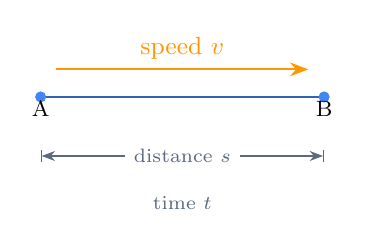
\begin{tikzpicture}[>=Stealth]
\draw[geo] (0,0)--(3.6,0);
\fill[tmBlue] (0,0) circle (2pt) (3.6,0) circle (2pt);
\node[lbl,below] at (0,0){A}; \node[lbl,below] at (3.6,0){B};
\draw[->,thick,tmOrange] (0.2,0.35)--node[above,font=\small]{speed $v$}(3.4,0.35);
\draw[|<->|,Slate] (0,-0.75)--node[fill=white,dim]{distance $s$}(3.6,-0.75);
\node[dim] at (1.8,-1.35){time $t$};
\end{tikzpicture}
\end{minipage}\par
\smallskip
\emph{Units:} distance in km and time in hours give speed in km/h; metres and minutes give m/min; metres and seconds give m/s. Always put the quantities in matching units before calculating.
\end{knowbox}

\shead{Units of time and of speed}
\begin{knowbox}
$1$ day $=24$ h;\quad $1$ h $=60$ min;\quad $1$ min $=60$ s;\quad $1$ h $=3\,600$ s.\par
\smallskip
-- Hours to minutes: multiply by $60$. \quad $0.4$ h $=0.4\times60$ min $=24$ min.\par
-- Minutes to hours: divide by $60$. \quad $1$ h $15$ min $=1\frac{15}{60}$ h $=1.25$ h.\par
\smallskip
\textbf{Changing units of speed:}\par
-- $54$ km/h: in $1$ hour $54\,000$ m, so in $1$ second $54\,000:3\,600=15$ m. So $54$ km/h $=15$ m/s.\par
-- In short: km/h $\to$ m/s: divide by $3.6$;\quad m/s $\to$ km/h: multiply by $3.6$.\par
-- $600$ m/min: in $1$ hour $600\times60=36\,000$ m $=36$ km. So $600$ m/min $=36$ km/h.
\end{knowbox}

\shead{Working with times of day}
\begin{knowbox}
\begin{minipage}[t]{0.58\linewidth}
When a journey has a departure time, an arrival time and a stop:\par
\smallskip
travel time $=$ arrival time $-$ departure time $-$ stopping time;\par
arrival time $=$ departure time $+$ travel time $+$ stopping time.\par
\smallskip
When adding or subtracting times, work with hours and minutes separately; $60$ min make $1$ h.\par
\smallskip
To use $s=v\times t$, write the travel time in hours (as a decimal or a fraction).
\end{minipage}\hfill
\begin{minipage}[t]{0.38\linewidth}\vspace{4pt}\centering
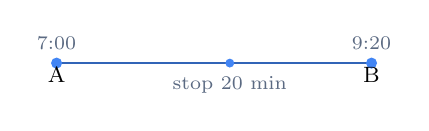
\begin{tikzpicture}[>=Stealth]
\draw[geo] (0,0)--(4,0);
\fill[tmBlue] (0,0) circle (2pt) (4,0) circle (2pt) (2.2,0) circle (1.6pt);
\node[lbl,below] at (0,0){A}; \node[lbl,below] at (4,0){B};
\node[dim,above] at (0,0.05){7:00}; \node[dim,above] at (4,0.05){9:20};
\node[dim,below] at (2.2,-0.05){stop $20$ min};
\end{tikzpicture}\par\smallskip
{\small travel time $=9$ h $20$ min $-\ 7$ h $-\ 20$ min $=2$ h}
\end{minipage}
\end{knowbox}
\gap
\begin{exbox}{\ExWord\ 1}
Fill in the blanks.
\begin{cols3}
\pa{a} $0.75$ h $=\dots$ min; & \pa{b} $2$ h $24$ min $=\dots$ h; & \pa{c} $3$ min $12$ s $=\dots$ s.
\end{cols3}
\guide
\pa{a} $0.75$ h $=0.75\times60$ min $=45$ min.\par
\pa{b} $24$ min $=24:60$ h $=0.4$ h, so $2$ h $24$ min $=2.4$ h.\par
\pa{c} $3$ min $=3\times60=180$ s, so $3$ min $12$ s $=180+12=192$ s.
\dapso{\pa{a} $45$ min;\par \pa{b} $2.4$ h;\par \pa{c} $192$ s.}
\end{exbox}
\gap
\begin{exbox}{\ExWord\ 2}
Fill in the blanks.
\begin{cols3}
\pa{a} $72$ km/h $=\dots$ m/s; & \pa{b} $15$ m/s $=\dots$ km/h; & \pa{c} $800$ m/min $=\dots$ km/h.
\end{cols3}
\guide
\pa{a} $72$ km $=72\,000$ m; $1$ h $=3\,600$ s.\par $72\,000:3\,600=20$, so $72$ km/h $=20$ m/s.\par
\pa{b} In $1$ hour: $15\times3\,600=54\,000$ m $=54$ km. So $15$ m/s $=54$ km/h.\par
\pa{c} In $1$ hour: $800\times60=48\,000$ m $=48$ km. So $800$ m/min $=48$ km/h.
\dapso{\pa{a} $20$ m/s;\par \pa{b} $54$ km/h;\par \pa{c} $48$ km/h.}
\end{exbox}
\gap
\begin{exbox}{\ExWord\ 3}
A coach leaves town A at 6:45 and reaches town B, $110$ km away, at 9:15. On the way it stops for $30$ min. Find the speed of the coach.
\guide
From 6:45 to 9:15: $9$ h $15$ min $-\ 6$ h $45$ min $=2$ h $30$ min.\par
Travel time: $2$ h $30$ min $-\ 30$ min $=2$ h.\par
Speed: $110:2=55$ km/h.
\dapso{$55$ km/h.}
\end{exbox}
\gap
\begin{exbox}{\ExWord\ 4}
Hùng cycles from home at 7:20 at $14$ km/h and arrives at his grandparents' house at 9:05 without stopping. How far is it from his home to his grandparents' house?
\guide
Travel time: $9$ h $5$ min $-\ 7$ h $20$ min $=1$ h $45$ min.\par
$1$ h $45$ min $=1\frac{45}{60}$ h $=1.75$ h.\par
Distance: $14\times1.75=24.5$ km.
\dapso{$24.5$ km.}
\end{exbox}
\gap
\begin{exbox}{\ExWord\ 5}
\begin{minipage}[t]{0.56\linewidth}
At 6:30 a lorry leaves A for B, $135$ km away, at $45$ km/h. At B it stops for $40$ min to unload, then drives back to A at $54$ km/h. At what time does it get back to A?
\end{minipage}\hfill
\begin{minipage}[t]{0.4\linewidth}\vspace{2pt}\centering
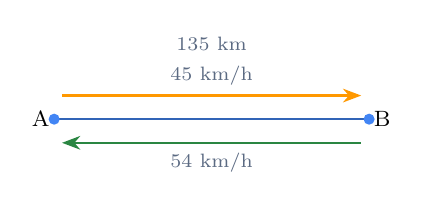
\begin{tikzpicture}[>=Stealth]
\draw[geo] (0,0)--(4,0);
\fill[tmBlue] (0,0) circle (2pt) (4,0) circle (2pt);
\node[lbl,left] at (0,0){A}; \node[lbl,right] at (4,0){B};
\draw[->,tmOrange,thick] (0.1,0.3)--node[above,dim]{$45$ km/h}(3.9,0.3);
\draw[<-,tmGreen!80!black,thick] (0.1,-0.3)--node[below,dim]{$54$ km/h}(3.9,-0.3);
\node[dim,above] at (2,0.75){$135$ km};
\end{tikzpicture}
\end{minipage}
\guide
Time from A to B: $135:45=3$ h.\par
Time from B back to A: $135:54=2.5$ h $=2$ h $30$ min.\par
Back at A: 6:30 $+\ 3$ h $+\ 40$ min $+\ 2$ h $30$ min $=$ 12:40.
\dapso{12:40.}
\end{exbox}
\dividerbar{Practice}
\begin{probbox}{1}{\relax}
Fill in the blanks.
\begin{cols2}
\pa{a} $0.4$ h $=\dots$ min; & \pa{b} $1.25$ h $=\dots$ min;\\
\pa{c} $2$ h $18$ min $=\dots$ h; & \pa{d} $45$ min $=\dots$ h.
\end{cols2}
\end{probbox}
\probsol{
\pa{a} $0.4\times60=24$ min.\par \pa{b} $1.25\times60=75$ min.\par \pa{c} $18:60=0.3$, so $2.3$ h.\par \pa{d} $45:60=0.75$ h.
\dapso{$24$ min; $75$ min; $2.3$ h; $0.75$ h.}}
\gap
\begin{probbox}{2}{\relax}
Fill in the blanks.
\begin{cols2}
\pa{a} $3.5$ min $=\dots$ s; & \pa{b} $2$ min $15$ s $=\dots$ s;\\
\pa{c} $1.5$ days $=\dots$ h; & \pa{d} $150$ s $=\dots$ min.
\end{cols2}
\end{probbox}
\probsol{
\pa{a} $3.5\times60=210$ s.\par \pa{b} $2\times60+15=135$ s.\par \pa{c} $1.5\times24=36$ h.\par \pa{d} $150:60=2.5$ min.
\dapso{$210$ s; $135$ s; $36$ h; $2.5$ min.}}
\gap
\begin{probbox}{3}{\relax}
Fill in the blanks.
\begin{cols2}
\pa{a} $36$ km/h $=\dots$ m/s; & \pa{b} $25$ m/s $=\dots$ km/h;\\
\pa{c} $54$ km/h $=\dots$ m/min; & \pa{d} $750$ m/min $=\dots$ km/h.
\end{cols2}
\end{probbox}
\probsol{
\pa{a} $36\,000:3\,600=10$ m/s.\par
\pa{b} $25\times3\,600=90\,000$ m $=90$ km, so $90$ km/h.\par
\pa{c} $54\,000:60=900$ m/min.\par
\pa{d} $750\times60=45\,000$ m $=45$ km, so $45$ km/h.
\dapso{$10$ m/s; $90$ km/h; $900$ m/min; $45$ km/h.}}
\gap
\begin{probbox}{4}{\relax}
Work out.
\begin{cols2}
\pa{a} $3$ h $45$ min $+\ 2$ h $30$ min; & \pa{b} $8$ h $10$ min $-\ 5$ h $35$ min;\\
\pa{c} $1$ h $25$ min $\times\ 3$; & \pa{d} $7$ h $30$ min $:\ 6$.
\end{cols2}
\end{probbox}
\probsol{
\pa{a} $5$ h $75$ min $=6$ h $15$ min.\par
\pa{b} $8$ h $10$ min $=7$ h $70$ min; $7$ h $70$ min $-\ 5$ h $35$ min $=2$ h $35$ min.\par
\pa{c} $3$ h $75$ min $=4$ h $15$ min.\par
\pa{d} $7$ h $30$ min $=450$ min; $450:6=75$ min $=1$ h $15$ min.
\dapso{$6$ h $15$ min; $2$ h $35$ min; $4$ h $15$ min; $1$ h $15$ min.}}
\gap
\begin{probbox}{5}{\relax}
A car travels $150$ km in $3$ hours. Find its speed.
\end{probbox}
\probsol{
Speed: $150:3=50$ km/h.
\dapso{$50$ km/h.}}
\gap
\begin{probbox}{6}{\relax}
A cyclist rides $31.5$ km in $2$ h $15$ min. Find the cyclist's speed.
\end{probbox}
\probsol{
$2$ h $15$ min $=2.25$ h.\par
Speed: $31.5:2.25=14$ km/h.
\dapso{$14$ km/h.}}
\gap
\begin{probbox}{7}{\relax}
Lan runs one lap of a $400$ m track in $50$ seconds. Find her speed in m/s.
\end{probbox}
\probsol{
Speed: $400:50=8$ m/s.
\dapso{$8$ m/s.}}
\gap
\begin{probbox}{8}{\relax}
A car travels at $48$ km/h for $2.5$ hours. How far does it go?
\end{probbox}
\probsol{
Distance: $48\times2.5=120$ km.
\dapso{$120$ km.}}
\gap
\begin{probbox}{9}{\relax}
Grandma walks at $4.5$ km/h for $1$ h $20$ min. How far does she walk?
\end{probbox}
\probsol{
$1$ h $20$ min $=1\frac{20}{60}$ h $=\frac43$ h.\par
Distance: $4.5\times\frac43=6$ km.
\dapso{$6$ km.}}
\gap
\begin{probbox}{10}{\relax}
A motorbike travels $84$ km at $35$ km/h. How long does the journey take?
\end{probbox}
\probsol{
Time: $84:35=2.4$ h.\par
$0.4$ h $=0.4\times60=24$ min, so $2.4$ h $=2$ h $24$ min.
\dapso{$2$ h $24$ min.}}
\gap
\begin{probbox}{11}{\relax}
A swallow flies at $108$ km/h. How many minutes does it need to fly $27$ km?
\end{probbox}
\probsol{
Time: $27:108=0.25$ h.\par
$0.25$ h $=0.25\times60=15$ min.
\dapso{$15$ min.}}
\gap
\begin{probbox}{12}{\relax}
A coach leaves at 7:15 and arrives at 9:45 after travelling $125$ km without stopping. Find its speed.
\end{probbox}
\probsol{
Travel time: $9$ h $45$ min $-\ 7$ h $15$ min $=2$ h $30$ min $=2.5$ h.\par
Speed: $125:2.5=50$ km/h.
\dapso{$50$ km/h.}}
\gap
\begin{probbox}{13}{\relax}
A motorbike leaves at 13:40 and arrives at 15:10, riding at $42$ km/h without stopping. How long is the journey?
\end{probbox}
\probsol{
Travel time: $15$ h $10$ min $-\ 13$ h $40$ min $=1$ h $30$ min $=1.5$ h.\par
Distance: $42\times1.5=63$ km.
\dapso{$63$ km.}}
\gap
\begin{probbox}{14}{\relax}
A van leaves at 6:50 to travel $96$ km at $40$ km/h without stopping. At what time does it arrive?
\end{probbox}
\probsol{
Travel time: $96:40=2.4$ h $=2$ h $24$ min.\par
Arrival: 6:50 $+\ 2$ h $24$ min $=8$ h $74$ min $=$ 9:14.
\dapso{9:14.}}
\gap
\begin{probbox}{15}{\relax}
Mr Tâm must reach a city $150$ km away at 11:00. His car goes at $60$ km/h and he will not stop. At what time must he set off?
\end{probbox}
\probsol{
Travel time: $150:60=2.5$ h $=2$ h $30$ min.\par
Departure: $11$ h $-\ 2$ h $30$ min $=$ 8:30.
\dapso{8:30.}}
\gap
\begin{probbox}{16}{\relax}
A car leaves A at 7:00 and arrives at B, $162$ km away, at 10:20. On the way it stops for $20$ min. Find its speed.
\end{probbox}
\probsol{
From 7:00 to 10:20: $3$ h $20$ min.\par
Travel time: $3$ h $20$ min $-\ 20$ min $=3$ h.\par
Speed: $162:3=54$ km/h.
\dapso{$54$ km/h.}}
\gap
\begin{probbox}{17}{\relax}
A motorbike leaves at 8:15 at $36$ km/h and arrives at 11:30. On the way the rider stops for $45$ min. How long is the journey?
\end{probbox}
\probsol{
From 8:15 to 11:30: $3$ h $15$ min.\par
Travel time: $3$ h $15$ min $-\ 45$ min $=2$ h $30$ min $=2.5$ h.\par
Distance: $36\times2.5=90$ km.
\dapso{$90$ km.}}
\gap
\begin{probbox}{18}{\relax}
A motorcyclist rides $37.5$ km in $1$ h $15$ min. At the same speed, how long will $51$ km take?
\end{probbox}
\probsol{
$1$ h $15$ min $=1.25$ h.\par
Speed: $37.5:1.25=30$ km/h.\par
Time for $51$ km: $51:30=1.7$ h $=1$ h $42$ min.
\dapso{$1$ h $42$ min.}}
\gap
\begin{probbox}{19}{\relax}
A bus at $40$ km/h covers a road in $3$ h $30$ min. How long does a car at $56$ km/h take on the same road?
\end{probbox}
\probsol{
$3$ h $30$ min $=3.5$ h.\par
Length of the road: $40\times3.5=140$ km.\par
Time for the car: $140:56=2.5$ h $=2$ h $30$ min.
\dapso{$2$ h $30$ min.}}
\gap
\begin{probbox}{20}{\relax}
Mai walks $1.2$ km from home to school in $15$ min. Find her speed in km/h and in m/min.
\end{probbox}
\probsol{
$15$ min $=0.25$ h.\par
Speed: $1.2:0.25=4.8$ km/h.\par
$1.2$ km $=1\,200$ m; speed: $1\,200:15=80$ m/min.
\dapso{$4.8$ km/h; $80$ m/min.}}
\gap
\begin{probbox}{21}{\relax}
Hà cycles to school at $12$ km/h and needs $15$ min. On the same road, what speed would get her there in $10$ min?
\end{probbox}
\probsol{
$15$ min $=0.25$ h. Distance: $12\times0.25=3$ km.\par
$10$ min $=\frac{10}{60}$ h $=\frac16$ h.\par
Speed needed: $3:\frac16=18$ km/h.
\dapso{$18$ km/h.}}
\gap
\begin{probbox}{22}{\relax}
Sound travels through air at $340$ m/s. Bình hears the thunder $5$ seconds after he sees the lightning. About how far away is the storm? (Light arrives almost at once.)
\end{probbox}
\probsol{
Distance: $340\times5=1\,700$ m $=1.7$ km.
\dapso{About $1.7$ km.}}
\gap
\begin{probbox}{23}{\relax}
A night train leaves at 21:30 and runs $360$ km at $72$ km/h without stopping. At what time does it arrive?
\end{probbox}
\probsol{
Travel time: $360:72=5$ h.\par
$21$ h $30$ min $+\ 5$ h $=26$ h $30$ min, that is 2:30 the next morning.
\dapso{2:30 the next day.}}
\gap
\begin{probbox}{24}{\relax}
Quân cycles for $40$ min at $15$ km/h, then walks for $18$ min at $5$ km/h. How far does he go altogether?
\end{probbox}
\probsol{
Cycling: $40$ min $=\frac23$ h; $15\times\frac23=10$ km.\par
Walking: $18$ min $=0.3$ h; $5\times0.3=1.5$ km.\par
Altogether: $10+1.5=11.5$ km.
\dapso{$11.5$ km.}}
\gap
\begin{probbox}{25}{\relax}
A taxi leaves A at 7:00 for B, $90$ km away, at $45$ km/h. It waits at B for $30$ min, then returns to A at $60$ km/h. At what time is it back at A?
\end{probbox}
\probsol{
A to B: $90:45=2$ h. B to A: $90:60=1.5$ h $=1$ h $30$ min.\par
Back at A: 7:00 $+\ 2$ h $+\ 30$ min $+\ 1$ h $30$ min $=$ 11:00.
\dapso{11:00.}}
\gap
\begin{probbox}{26}{\relax}
\begin{minipage}[t]{0.56\linewidth}
The road AB is $120$ km long. At 7:30 a car leaves A at $40$ km/h. After $2$ hours it stops for $15$ min to change a tyre, then covers the rest of the road at $50$ km/h. At what time does it reach B?
\end{minipage}\hfill
\begin{minipage}[t]{0.4\linewidth}\vspace{4pt}\centering
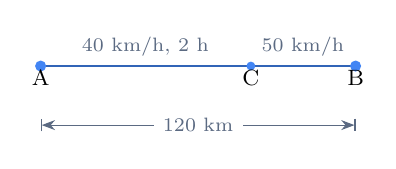
\begin{tikzpicture}[>=Stealth]
\draw[geo] (0,0)--(4,0);
\fill[tmBlue] (0,0) circle (2pt) (4,0) circle (2pt) (2.67,0) circle (1.6pt);
\node[lbl,below] at (0,0){A}; \node[lbl,below] at (4,0){B}; \node[lbl,below] at (2.67,0){C};
\node[dim,above] at (1.33,0){$40$ km/h, $2$ h}; \node[dim,above] at (3.33,0){$50$ km/h};
\draw[|<->|,Slate] (0,-0.75)--node[fill=white,dim]{$120$ km}(4,-0.75);
\end{tikzpicture}
\end{minipage}
\end{probbox}
\probsol{
Distance in the first $2$ h: $40\times2=80$ km.\par
Rest of the road: $120-80=40$ km.\par
Time for it: $40:50=0.8$ h $=48$ min.\par
Arrival: 7:30 $+\ 2$ h $+\ 15$ min $+\ 48$ min $=$ 10:33.
\dapso{10:33.}}
\gap
\begin{probbox}{27}{\relax}
At 6:30 Mr Phúc walks from his house at $5$ km/h. At 7:06 he gets on a bus, which goes at $40$ km/h and arrives at the market town at 7:51. How far is the market town from his house?
\end{probbox}
\probsol{
Walking time: $7$ h $6$ min $-\ 6$ h $30$ min $=36$ min $=0.6$ h; walking: $5\times0.6=3$ km.\par
Bus time: $7$ h $51$ min $-\ 7$ h $6$ min $=45$ min $=0.75$ h; bus: $40\times0.75=30$ km.\par
Distance: $3+30=33$ km.
\dapso{$33$ km.}}
\gap
\begin{probbox}{28}{\relax}
A car covers $180$ km in $2$ h $30$ min. Find its speed in km/h and in m/s.
\end{probbox}
\probsol{
$2$ h $30$ min $=2.5$ h.\par
Speed: $180:2.5=72$ km/h.\par
$72$ km/h $=72\,000:3\,600=20$ m/s.
\dapso{$72$ km/h; $20$ m/s.}}
\gap
\begin{probbox}{29}{\relax}
A snail crawls at $15$ cm/min. How many minutes does it need to cross a path $1.2$ m wide?
\end{probbox}
\probsol{
$1.2$ m $=120$ cm.\par
Time: $120:15=8$ min.
\dapso{$8$ min.}}
\gap
\begin{probbox}{30}{\relax}
A ferry leaves at 22:45 and arrives at 4:15 the next morning without stopping, after sailing $132$ km. Find its speed.
\end{probbox}
\probsol{
From 22:45 to 24:00: $1$ h $15$ min; from 0:00 to 4:15: $4$ h $15$ min.\par
Travel time: $1$ h $15$ min $+\ 4$ h $15$ min $=5$ h $30$ min $=5.5$ h.\par
Speed: $132:5.5=24$ km/h.
\dapso{$24$ km/h.}}
\dividerbar{Challenge -- Extension}
\begin{probbox}{31}{\stars{1}}
The road AB is $150$ km long. At 7:30 a car leaves A. It covers the first $\dfrac13$ of the road at $40$ km/h and the rest at $50$ km/h. At what time does it reach B?
\end{probbox}
\probsol{
First part: $150:3=50$ km; time $50:40=1.25$ h $=1$ h $15$ min.\par
Rest: $150-50=100$ km; time $100:50=2$ h.\par
Arrival: 7:30 $+\ 1$ h $15$ min $+\ 2$ h $=$ 10:45.
\dapso{10:45.}}
\gap
\begin{probbox}{32}{\stars{1}}
A cyclist rides for $2$ h $15$ min at $16$ km/h, then for $1$ h $45$ min at $12$ km/h. How far does she ride in all? On average, how many kilometres does she ride per hour?
\end{probbox}
\probsol{
First part: $16\times2.25=36$ km. Second part: $12\times1.75=21$ km.\par
In all: $36+21=57$ km in $2.25+1.75=4$ h.\par
On average: $57:4=14.25$ km per hour.
\dapso{$57$ km; $14.25$ km/h.}}
\gap
\begin{probbox}{33}{\stars{1}}
A road has an uphill part of $9$ km and a downhill part of $15$ km. A cyclist goes uphill at $12$ km/h and downhill at $30$ km/h. How long does the whole road take? What is the average speed over the whole road?
\end{probbox}
\probsol{
Uphill: $9:12=0.75$ h. Downhill: $15:30=0.5$ h.\par
Whole road: $0.75+0.5=1.25$ h $=1$ h $15$ min.\par
Average speed: $(9+15):1.25=19.2$ km/h.
\dapso{$1$ h $15$ min; $19.2$ km/h.}}
\gap
\begin{probbox}{34}{\stars{1}}
A train leaves at 23:40 and runs for $2$ h $50$ min at $60$ km/h. It stops at a station for $20$ min, then runs another $75$ km at $50$ km/h to the last station. At what time does it arrive, and how long is the whole route?
\end{probbox}
\probsol{
First part: $2$ h $50$ min $=2\frac56$ h; $60\times2\frac56=170$ km.\par
Second part: $75:50=1.5$ h $=1$ h $30$ min.\par
Arrival: 23:40 $+\ 2$ h $50$ min $+\ 20$ min $+\ 1$ h $30$ min $=28$ h $20$ min, that is 4:20 the next day.\par
Whole route: $170+75=245$ km.
\dapso{4:20 the next day; $245$ km.}}
\gap
\begin{probbox}{35}{\stars{1}}
Hoa jogs $3$ laps of a $400$ m track in $6$ min. Find her speed in m/min and in km/h.
\end{probbox}
\probsol{
Distance: $400\times3=1\,200$ m.\par
Speed: $1\,200:6=200$ m/min.\par
In $1$ hour: $200\times60=12\,000$ m $=12$ km, so $12$ km/h.
\dapso{$200$ m/min; $12$ km/h.}}
\gap
\begin{probbox}{36}{\stars{1}}
A car moves at $15$ m/s. How many kilometres does it cover in $1$ h $20$ min?
\end{probbox}
\probsol{
$15$ m/s $=15\times3.6=54$ km/h.\par
$1$ h $20$ min $=\frac43$ h.\par
Distance: $54\times\frac43=72$ km.
\dapso{$72$ km.}}
\gap
\begin{probbox}{37}{\stars{1}}
At 8:15 a motorbike leaves A at $36$ km/h. At 9:35 the rider speeds up by $9$ km/h and keeps that speed until reaching B at 10:55. How far is it from A to B?
\end{probbox}
\probsol{
From 8:15 to 9:35: $1$ h $20$ min $=\frac43$ h; distance $36\times\frac43=48$ km.\par
New speed: $36+9=45$ km/h.\par
From 9:35 to 10:55: $1$ h $20$ min $=\frac43$ h; distance $45\times\frac43=60$ km.\par
AB: $48+60=108$ km.
\dapso{$108$ km.}}
\gap
\begin{probbox}{38}{\stars{1}}
The road AB is $108$ km long. A lorry leaves A for B at 7:00 at $36$ km/h. A car leaves A at 7:30 at $54$ km/h. Which arrives at B first, and by how many minutes?
\end{probbox}
\probsol{
Lorry: $108:36=3$ h, arriving at 10:00.\par
Car: $108:54=2$ h, arriving at 7:30 $+\ 2$ h $=$ 9:30.\par
The car arrives first, $30$ min before the lorry.
\dapso{The car, $30$ min earlier.}}
\gap
\begin{probbox}{39}{\stars{1}}
An runs $100$ m in $16$ s. Bình runs $1$ km in $3$ min $20$ s. Cường cycles at $21.6$ km/h. Order the three boys from fastest to slowest.
\end{probbox}
\probsol{
An: $100:16=6.25$ m/s.\par
Bình: $3$ min $20$ s $=200$ s; $1\,000:200=5$ m/s.\par
Cường: $21.6$ km/h $=21.6:3.6=6$ m/s.\par
$6.25>6>5$.
\dapso{An, Cường, Bình.}}
\gap
\begin{probbox}{40}{\stars{1}}
Tuấn's school is $4$ km from home and lessons start at 7:15.\par
\pa{a} He leaves at 6:40 and cycles at $12$ km/h. How many minutes early is he?\par
\pa{b} One day he leaves at 6:59. What speed must he ride at to arrive exactly at 7:15?
\end{probbox}
\probsol{
\pa{a} Time: $4:12=\frac13$ h $=20$ min; he arrives at 7:00, that is $15$ min early.\par
\pa{b} He has $16$ min $=\frac{16}{60}$ h $=\frac4{15}$ h.\par
Speed: $4:\frac4{15}=15$ km/h.
\dapso{\pa{a} $15$ min;\par \pa{b} $15$ km/h.}}
\gap
\begin{probbox}{41}{\stars{1}}
A car leaves A at 7:05 and reaches B at 9:41. On the way it stops for $18$ min. Its speed is $45$ km/h. Find the distance AB.
\end{probbox}
\probsol{
From 7:05 to 9:41: $2$ h $36$ min.\par
Travel time: $2$ h $36$ min $-\ 18$ min $=2$ h $18$ min $=2.3$ h.\par
AB: $45\times2.3=103.5$ km.
\dapso{$103.5$ km.}}
\gap
\begin{probbox}{42}{\stars{1}}
A plane flies at $840$ km/h. It takes off at 6:50 for a city $1\,260$ km away. At what time does it land?
\end{probbox}
\probsol{
Flying time: $1\,260:840=1.5$ h $=1$ h $30$ min.\par
Landing: 6:50 $+\ 1$ h $30$ min $=$ 8:20.
\dapso{8:20.}}
\gap
\begin{probbox}{43}{\stars{1}}
A runner covers $3$ km in $12$ min $30$ s. Find the speed in m/s and in km/h.
\end{probbox}
\probsol{
$12$ min $30$ s $=750$ s; $3$ km $=3\,000$ m.\par
Speed: $3\,000:750=4$ m/s.\par
$4$ m/s $=4\times3.6=14.4$ km/h.
\dapso{$4$ m/s; $14.4$ km/h.}}
\gap
\begin{probbox}{44}{\stars{1}}
Bình cycles for $45$ min at $16$ km/h; then his bike breaks and he walks the remaining $2.4$ km in $36$ min. How long is the whole road, and how fast did he walk?
\end{probbox}
\probsol{
Cycling: $45$ min $=0.75$ h; $16\times0.75=12$ km.\par
Whole road: $12+2.4=14.4$ km.\par
Walking: $36$ min $=0.6$ h; speed $2.4:0.6=4$ km/h.
\dapso{$14.4$ km; $4$ km/h.}}
\gap
\begin{probbox}{45}{\stars{2}}
The road AB is $60$ km long. A car spends half of its travel time at $40$ km/h and the other half at $60$ km/h. How long does it take from A to B?
\end{probbox}
\probsol{
In each hour of the first half it covers $40$ km, in each hour of the second half $60$ km.\par
One hour of the first half together with one hour of the second half covers $40+60=100$ km.\par
So each half lasts $60:100=0.6$ h.\par
Total time: $0.6\times2=1.2$ h $=1$ h $12$ min.\par
\emph{Check:} $40\times0.6+60\times0.6=24+36=60$ km.
\dapso{$1$ h $12$ min.}}
\gap
\begin{probbox}{46}{\stars{2}}
The road AB is $60$ km long. A car covers the first half of the road at $30$ km/h and the second half at $60$ km/h. Find the total time and the average speed. Is the average speed $45$ km/h?
\end{probbox}
\probsol{
Each half: $30$ km.\par
First half: $30:30=1$ h; second half: $30:60=0.5$ h.\par
Total time: $1.5$ h.\par
Average speed: $60:1.5=40$ km/h, not $45$ km/h (the car spends longer at the slower speed).
\dapso{$1.5$ h; $40$ km/h (no).}}
\gap
\begin{probbox}{47}{\stars{1}}
On a motorway, Dad's car passes one kilometre post every $48$ seconds. What is its speed in km/h?
\end{probbox}
\probsol{
$1$ h $=3\,600$ s. In $1$ hour it passes $3\,600:48=75$ posts.\par
Speed: $75$ km/h.
\dapso{$75$ km/h.}}
\gap
\begin{probbox}{48}{\stars{2}}
A tortoise and a hare race over $120$ m. The tortoise crawls steadily at $0.2$ m/s. The hare runs at $6$ m/s, stops after $90$ m to sleep, then wakes up and runs the last $30$ m at the same speed. At most how long can the hare sleep and still not lose?
\end{probbox}
\probsol{
Tortoise: $120:0.2=600$ s.\par
Hare running: $120:6=20$ s in all.\par
Longest sleep: $600-20=580$ s $=9$ min $40$ s.
\dapso{$9$ min $40$ s.}}
\gap
\begin{probbox}{49}{\stars{2}}
A train leaves station A at 19:20 and reaches station B, $570$ km away, at 6:05 the next day. Its stops at stations add up to $1$ h $15$ min. Find the speed of the train while it is moving.
\end{probbox}
\probsol{
From 19:20 to 6:05 the next day: $4$ h $40$ min $+\ 6$ h $5$ min $=10$ h $45$ min.\par
Moving time: $10$ h $45$ min $-\ 1$ h $15$ min $=9$ h $30$ min $=9.5$ h.\par
Speed: $570:9.5=60$ km/h.
\dapso{$60$ km/h.}}
\gap
\begin{probbox}{50}{\stars{2}}
The road AB is $115$ km long. A car leaves A at 7:00 and must reach B at 9:30. For the first $1$ h $15$ min it goes at $40$ km/h. At what speed must it cover the rest of the road?
\end{probbox}
\probsol{
Distance so far: $40\times1.25=50$ km; still to go: $115-50=65$ km.\par
Time left: $9$ h $30$ min $-\ 7$ h $-\ 1$ h $15$ min $=1$ h $15$ min $=1.25$ h.\par
Speed needed: $65:1.25=52$ km/h.
\dapso{$52$ km/h.}}
\clearpage
\titlehead
\begingroup\setbox0=\vbox{\section*{Meeting and Catching Up}}\endgroup
\chapterhead{7}{Meeting and Catching Up}
\shead{Two objects moving towards each other}
\begin{knowbox}
Two objects start \emph{at the same time} from $A$ and $B$, a distance $s$ apart, and move towards each other with speeds $v_1$ and $v_2$.
\begin{barfigC}
\draw[geo] (0,0)--(7,0);
\draw[geo] (0,0.12)--(0,-0.12) (7,0.12)--(7,-0.12);
\node[lbl,above] at (0,0.12){$A$}; \node[lbl,above] at (7,0.12){$B$};
\draw[->,line width=1pt,tmOrange] (0.1,-0.35)--(1.5,-0.35); \node[dim,below] at (0.8,-0.4){$v_1$};
\draw[->,line width=1pt,tmGreen] (6.9,-0.35)--(5.5,-0.35); \node[dim,below] at (6.2,-0.4){$v_2$};
\fill[AnsRed] (4,0) circle (2.2pt); \node[lbl,above] at (4,0.12){$C$};
\brcup{0}{7}{0.7}{$s$}
\end{barfigC}
\begin{itemize}[leftmargin=1.4em,itemsep=3pt]
\item Every hour the gap between them shrinks by $v_1+v_2$ (the \emph{closing speed}).
\item Time until they meet: $\ t=s:(v_1+v_2)$.
\item The meeting point $C$ is $v_1\times t$ from $A$ and $v_2\times t$ from $B$.
\item Clock time of meeting $=$ starting time $+\ t$.
\item If one object sets off earlier, first find how far it has gone by the time the other one starts; the \emph{remaining} distance is then shared as above.
\end{itemize}
\end{knowbox}
\gap
\shead{Two objects moving in the same direction}
\begin{knowbox}
Two objects start \emph{at the same time} from $A$ and $B$ ($s$ apart) and move in the same direction $A\to B$; the one behind is faster: $v_1>v_2$.
\begin{barfigC}
\draw[geo] (0,0)--(7.2,0);
\draw[geo] (0,0.12)--(0,-0.12) (2.6,0.12)--(2.6,-0.12);
\node[lbl,above] at (0,0.12){$A$}; \node[lbl,above] at (2.6,0.12){$B$};
\draw[->,line width=1pt,tmOrange] (0.1,-0.35)--(1.7,-0.35); \node[dim,below] at (0.9,-0.4){$v_1$};
\draw[->,line width=1pt,tmGreen] (2.7,-0.35)--(3.6,-0.35); \node[dim,below] at (3.15,-0.4){$v_2$};
\fill[AnsRed] (6.4,0) circle (2.2pt); \node[lbl,above] at (6.4,0.12){$C$};
\brcup{0}{2.6}{0.7}{$s$}
\end{barfigC}
\begin{itemize}[leftmargin=1.4em,itemsep=3pt]
\item Every hour the faster one gains $v_1-v_2$ on the slower one.
\item Time to catch up: $\ t=s:(v_1-v_2)$; the catching point is $v_1\times t$ from $A$.
\item If both start from the \emph{same place} at \emph{different times}, the head start is $s=v_2\times$ (difference in starting times).
\end{itemize}
\textbf{Note:} use the same units throughout (km, h, km/h or m, min, m/min). Two objects moving \emph{away} from each other (opposite directions from the same point) separate by $v_1+v_2$ every hour.
\end{knowbox}
\gap
\begin{exbox}{\ExWord\ 1}
Two towns $A$ and $B$ are $225$ km apart. At 6:45 a car leaves $A$ for $B$ at $48$ km/h; at the same time a coach leaves $B$ for $A$ at $42$ km/h. At what time do they meet, and how far from $A$ is the meeting point?
\guide
\begin{barfigC}
\draw[geo] (0,0)--(7,0);
\draw[geo] (0,0.12)--(0,-0.12) (7,0.12)--(7,-0.12);
\node[lbl,above] at (0,0.12){$A$}; \node[lbl,above] at (7,0.12){$B$};
\draw[->,line width=1pt,tmOrange] (0.1,-0.35)--(1.5,-0.35); \node[dim,below] at (0.8,-0.4){$48$ km/h};
\draw[->,line width=1pt,tmGreen] (6.9,-0.35)--(5.5,-0.35); \node[dim,below] at (6.2,-0.4){$42$ km/h};
\fill[AnsRed] (3.73,0) circle (2.2pt); \node[lbl,above] at (3.73,0.12){$C$};
\brcup{0}{7}{0.7}{$225$ km}
\end{barfigC}
Every hour the two vehicles close up: $48+42=90$ (km).\par
Time until they meet: $225:90=2.5$ (h) $=2$ h $30$ min.\par
They meet at: 6:45 $+\ 2$ h $30$ min $=$ 9:15.\par
The meeting point is $48\times2.5=120$ (km) from $A$.
\ans{9:15; $120$ km from $A$.}
\end{exbox}
\gap
\begin{exbox}{\ExWord\ 2}
At 7:10 Lan leaves school by bicycle at $12$ km/h. At 7:40 her brother leaves the school on a motorbike at $36$ km/h and rides after her along the same road. At what time does he catch up with her, and how far from school?
\guide
Lan's head start in time: 7:40 $-$ 7:10 $=30$ min $=0.5$ h.\par
Distance Lan has covered by 7:40: $12\times0.5=6$ (km).\par
Every hour the motorbike gains: $36-12=24$ (km).\par
Time to catch up: $6:24=0.25$ (h) $=15$ min. \ They meet at 7:40 $+\ 15$ min $=$ 7:55.\par
Distance from school: $36\times0.25=9$ (km).
\ans{7:55; $9$ km from school.}
\end{exbox}
\gap
\begin{exbox}{\ExWord\ 3}
Points $A$ and $B$ are $18$ km apart. At 6:30 a motorbike leaves $A$ at $42$ km/h and, at the same time, a cyclist leaves $B$ at $15$ km/h; both travel in the direction from $A$ to $B$. At what time does the motorbike catch the cyclist, and how far from $A$?
\guide
\begin{barfigC}
\draw[geo] (0,0)--(4.6,0);
\draw[geo] (0,0.12)--(0,-0.12) (2.4,0.12)--(2.4,-0.12);
\node[lbl,above] at (0,0.12){$A$}; \node[lbl,above] at (2.4,0.12){$B$};
\draw[->,line width=1pt,tmOrange] (0.1,-0.35)--(1.7,-0.35); \node[dim,below] at (0.9,-0.4){$42$ km/h};
\draw[->,line width=1pt,tmGreen] (2.5,-0.35)--(3.4,-0.35); \node[dim,below] at (3.1,-0.4){$15$ km/h};
\fill[AnsRed] (3.73,0) circle (2.2pt); \node[lbl,above] at (3.73,0.12){$C$};
\brcup{0}{2.4}{0.7}{$18$ km}
\end{barfigC}
Every hour the motorbike gains: $42-15=27$ (km).\par
Time to catch up: $18:27=\dfrac23$ (h) $=40$ min. \ It catches up at 6:30 $+\ 40$ min $=$ 7:10.\par
Distance from $A$: $42\times\dfrac23=28$ (km).
\ans{7:10; $28$ km from $A$.}
\end{exbox}
\gap
\begin{exbox}{\ExWord\ 4}
Two towns are $180$ km apart. A car and a motorbike set off from the two towns at the same time towards each other and meet after $2$ hours. The car is $10$ km/h faster than the motorbike. Find the speed of each.
\guide
Sum of the two speeds (the closing speed): $180:2=90$ (km/h).
\begin{barfigC}
\rowlab{-0.15}{0.62}{Motorbike:}
\blk{0}{3.2}{0.62}{0.42}{tmBlue}{}
\rowlab{-0.15}{0}{Car:}
\blk{0}{3.2}{0}{0.42}{tmGreen}{}
\blk{3.2}{3.9}{0}{0.42}{tmOrange}{}
\brcdn{3.2}{3.9}{-0.32}{$10$ km/h}
\vbrace{4.1}{0.85}{-0.22}{$90$ km/h}
\end{barfigC}
Speed of the motorbike: $(90-10):2=40$ (km/h).\par
Speed of the car: $40+10=50$ (km/h).
\ans{car $50$ km/h, motorbike $40$ km/h.}
\end{exbox}
\gap
\begin{exbox}{\ExWord\ 5}
Two places are $150$ km apart. At 8:00 two cars leave them and drive towards each other at $35$ km/h and $40$ km/h. At what time are the two cars $30$ km apart?
\guide
Every hour the cars close up by $35+40=75$ (km). There are \emph{two} moments when they are $30$ km apart.\par
\textbf{Before they meet:} together they have driven $150-30=120$ (km); time: $120:75=1.6$ (h) $=1$ h $36$ min, so at 9:36.\par
\textbf{After they meet:} together they have driven $150+30=180$ (km); time: $180:75=2.4$ (h) $=2$ h $24$ min, so at 10:24.
\ans{at 9:36 and at 10:24.}
\end{exbox}
\dividerbar{Practice}
\begin{probbox}{1}{\relax}
Two villages are $36$ km apart. Two cyclists leave the villages at the same time and ride towards each other at $13$ km/h and $11$ km/h. After how long do they meet?
\end{probbox}
\probsol{
Closing speed: $13+11=24$ (km/h).\par Time: $36:24=1.5$ (h) $=1$ h $30$ min.
\dapso{$1$ h $30$ min.}}
\gap
\begin{probbox}{2}{\relax}
Road $AB$ is $279$ km long. At 7:20 a car leaves $A$ for $B$ at $68$ km/h; at the same time a coach leaves $B$ for $A$ at $56$ km/h. At what time do they meet?
\end{probbox}
\probsol{
Closing speed: $68+56=124$ (km/h).\par Time: $279:124=2.25$ (h) $=2$ h $15$ min.\par They meet at 7:20 $+\ 2$ h $15$ min $=$ 9:35.
\dapso{9:35.}}
\gap
\begin{probbox}{3}{\relax}
Two cities $A$ and $B$ are $168$ km apart. At the same moment a motorbike leaves $A$ at $38$ km/h and a car leaves $B$ at $46$ km/h, heading towards each other. After how long do they meet, and how far from $A$?
\end{probbox}
\probsol{
Closing speed: $38+46=84$ (km/h).\par Time: $168:84=2$ (h).\par Distance from $A$: $38\times2=76$ (km).
\dapso{after $2$ h, $76$ km from $A$.}}
\gap
\begin{probbox}{4}{\relax}
Two towns $A$ and $B$ are $210$ km apart. At 6:30 two cars leave $A$ and $B$ and drive towards each other, the car from $A$ at $45$ km/h and the car from $B$ at $39$ km/h. At what time do they meet, and how far from $A$ is the meeting point?
\end{probbox}
\probsol{
Closing speed: $45+39=84$ (km/h).\par Time: $210:84=2.5$ (h) $=2$ h $30$ min; they meet at 9:00.\par Distance from $A$: $45\times2.5=112.5$ (km).
\dapso{9:00; $112.5$ km from $A$.}}
\gap
\begin{probbox}{5}{\relax}
Two towns are $196$ km apart. A car and a motorbike leave the two towns at the same time towards each other and meet after $2$ h $20$ min. The car is $12$ km/h faster than the motorbike. Find the speed of each.
\end{probbox}
\probsol{
$2$ h $20$ min $=2\dfrac13$ h $=\dfrac73$ h.\par Sum of the speeds: $196:\dfrac73=84$ (km/h).\par
Motorbike: $(84-12):2=36$ (km/h); car: $36+12=48$ (km/h).
\dapso{car $48$ km/h, motorbike $36$ km/h.}}
\gap
\begin{probbox}{6}{\relax}
Two towns $A$ and $B$ are $245$ km apart. Two cars leave $A$ and $B$ at the same time towards each other and meet after $2.5$ h at a point $C$ that is $105$ km from $A$. Find the speed of each car.
\end{probbox}
\probsol{
Car from $A$: $105:2.5=42$ (km/h).\par Distance $CB$: $245-105=140$ (km).\par Car from $B$: $140:2.5=56$ (km/h).
\dapso{$42$ km/h and $56$ km/h.}}
\gap
\begin{probbox}{7}{\relax}
Road $AB$ is $288$ km long. A car and a motorbike leave $A$ and $B$ at the same time towards each other and meet after $3$ h $12$ min. The car's speed is $1.5$ times the motorbike's. Find the speed of each.
\end{probbox}
\probsol{
$3$ h $12$ min $=3.2$ h. \ Sum of the speeds: $288:3.2=90$ (km/h).\par
$1.5=\dfrac32$: motorbike $2$ parts, car $3$ parts; $5$ parts $=90$, one part $=18$ km/h.\par
Motorbike: $18\times2=36$ (km/h); car: $18\times3=54$ (km/h).
\dapso{car $54$ km/h, motorbike $36$ km/h.}}
\gap
\begin{probbox}{8}{\relax}
Road $AB$ is $270$ km long. At 7:00 a lorry leaves $A$ for $B$ at $40$ km/h. At 8:15 a car leaves $B$ for $A$ at $60$ km/h. At what time do they meet, and how far from $A$?
\end{probbox}
\probsol{
From 7:00 to 8:15 is $1$ h $15$ min $=1.25$ h; the lorry has gone $40\times1.25=50$ (km).\par
Remaining distance: $270-50=220$ (km). \ Closing speed: $40+60=100$ (km/h).\par
Time: $220:100=2.2$ (h) $=2$ h $12$ min; they meet at 8:15 $+\ 2$ h $12$ min $=$ 10:27.\par
Distance from $A$: $50+40\times2.2=138$ (km).
\dapso{10:27; $138$ km from $A$.}}
\gap
\begin{probbox}{9}{\relax}
At 6:30 a coach leaves $A$ for $B$ at $50$ km/h. Half an hour later a second coach leaves $B$ for $A$ at $45$ km/h. The two coaches meet at 9:00. How long is road $AB$?
\end{probbox}
\probsol{
First coach drives from 6:30 to 9:00: $2.5$ h, covering $50\times2.5=125$ (km).\par
Second coach starts at 7:00 and drives $2$ h, covering $45\times2=90$ (km).\par
$AB=125+90=215$ (km).
\dapso{$215$ km.}}
\gap
\begin{probbox}{10}{\relax}
Two places are $160$ km apart. Two cars leave them at the same time and drive towards each other at $38$ km/h and $42$ km/h. How far apart are they after $1$ h $30$ min?
\end{probbox}
\probsol{
Closing speed: $38+42=80$ (km/h).\par In $1.5$ h they close up $80\times1.5=120$ (km).\par Still apart: $160-120=40$ (km).
\dapso{$40$ km.}}
\gap
\begin{probbox}{11}{\relax}
Two cars leave $A$ and $B$ at the same time and drive towards each other. The first car needs $4$ h to drive the whole road $AB$; the second needs $6$ h. After $2$ h the cars are still $30$ km apart. How long is road $AB$?
\end{probbox}
\probsol{
In $1$ h the first car covers $\dfrac14$ of $AB$ and the second $\dfrac16$ of $AB$; together $\dfrac14+\dfrac16=\dfrac5{12}$ of $AB$.\par
In $2$ h together: $\dfrac5{12}\times2=\dfrac56$ of $AB$. \ Remaining: $1-\dfrac56=\dfrac16$ of $AB$, which is $30$ km.\par
$AB=30\times6=180$ (km).
\dapso{$180$ km.}}
\gap
\begin{probbox}{12}{\relax}
A motorbike needs $3$ h to ride from $A$ to $B$; a bicycle needs $6$ h to ride from $B$ to $A$. They set off at the same time towards each other. After how long do they meet?
\end{probbox}
\probsol{
In $1$ h together they cover $\dfrac13+\dfrac16=\dfrac12$ of $AB$.\par Time to cover the whole road together: $1:\dfrac12=2$ (h).
\dapso{$2$ h.}}
\gap
\begin{probbox}{13}{\relax}
Lan's house and Mai's house are $2.4$ km apart. At 16:40 the two girls leave home and walk towards each other, Lan at $4.5$ km/h and Mai at $3.5$ km/h. After how many minutes do they meet, and at what time?
\end{probbox}
\probsol{
Closing speed: $4.5+3.5=8$ (km/h).\par Time: $2.4:8=0.3$ (h) $=18$ min.\par They meet at 16:40 $+\ 18$ min $=$ 16:58.
\dapso{after $18$ min, at 16:58.}}
\gap
\begin{probbox}{14}{\relax}
$A$ and $B$ are $24$ km apart. A walker leaves $A$ at $4$ km/h and, at the same time, a cyclist leaves $B$ at $12$ km/h; they go towards each other. How far from $A$ do they meet?
\end{probbox}
\probsol{
Closing speed: $4+12=16$ (km/h).\par Time: $24:16=1.5$ (h).\par Distance from $A$: $4\times1.5=6$ (km).
\dapso{$6$ km.}}
\gap
\begin{probbox}{15}{\relax}
Road $AB$ is $132$ km long. A car leaves $A$ at $52$ km/h and, at the same time, a motorbike leaves $B$; they travel towards each other and meet after $1$ h $30$ min. Find the speed of the motorbike.
\end{probbox}
\probsol{
Sum of the speeds: $132:1.5=88$ (km/h).\par Motorbike: $88-52=36$ (km/h).
\dapso{$36$ km/h.}}
\gap
\begin{probbox}{16}{\relax}
$A$ and $B$ are $48$ km apart. At the same time a car leaves $A$ at $58$ km/h and a motorbike leaves $B$ at $42$ km/h, both going in the direction from $A$ to $B$. After how long does the car catch the motorbike, and how far from $A$?
\end{probbox}
\probsol{
The car gains $58-42=16$ (km) every hour.\par Time: $48:16=3$ (h).\par Distance from $A$: $58\times3=174$ (km).
\dapso{after $3$ h, $174$ km from $A$.}}
\gap
\begin{probbox}{17}{\relax}
At 6:40 a cyclist leaves a town at $14$ km/h. At 7:10 a motorbike leaves the same place at $35$ km/h and follows the same road. At what time does the motorbike catch the cyclist?
\end{probbox}
\probsol{
Head start in time: $30$ min $=0.5$ h; head start in distance: $14\times0.5=7$ (km).\par
The motorbike gains $35-14=21$ (km) every hour.\par Time: $7:21=\dfrac13$ (h) $=20$ min; it catches up at 7:30.
\dapso{7:30.}}
\gap
\begin{probbox}{18}{\relax}
A car leaves $A$ and a bicycle leaves $B$ at the same time, both going in the direction from $A$ to $B$. The car drives at $52$ km/h and the bicycle at $16$ km/h. The car catches the bicycle after $1$ h $45$ min. How far apart are $A$ and $B$?
\end{probbox}
\probsol{
The car gains $52-16=36$ (km) every hour.\par $1$ h $45$ min $=1.75$ h. \ $AB=36\times1.75=63$ (km).
\dapso{$63$ km.}}
\gap
\begin{probbox}{19}{\relax}
A cyclist riding at $15$ km/h has already covered $15$ km when a motorbike sets off after him from the same starting point at $40$ km/h. After how many minutes does the motorbike catch the cyclist?
\end{probbox}
\probsol{
The motorbike gains $40-15=25$ (km) every hour.\par Time: $15:25=0.6$ (h) $=36$ min.
\dapso{$36$ min.}}
\gap
\begin{probbox}{20}{\relax}
At 8:00 a lorry leaves $A$ at $45$ km/h. At 9:20 a car leaves $A$ at $75$ km/h along the same road. At what time does the car catch the lorry, and how far from $A$?
\end{probbox}
\probsol{
From 8:00 to 9:20 is $1$ h $20$ min $=\dfrac43$ h; the lorry is $45\times\dfrac43=60$ (km) ahead.\par
The car gains $75-45=30$ (km) every hour. \ Time: $60:30=2$ (h); it catches up at 11:20.\par
Distance from $A$: $75\times2=150$ (km).
\dapso{11:20; $150$ km from $A$.}}
\gap
\begin{probbox}{21}{\relax}
$A$ and $B$ are $36$ km apart. Two cars leave $A$ and $B$ at the same time in the same direction (from $A$ to $B$). After $3$ h the car from $A$ catches the car from $B$. The sum of their speeds is $84$ km/h. Find the speed of each car.
\end{probbox}
\probsol{
Difference of the speeds: $36:3=12$ (km/h).\par
Car from $A$: $(84+12):2=48$ (km/h); car from $B$: $48-12=36$ (km/h).
\dapso{$48$ km/h and $36$ km/h.}}
\gap
\begin{probbox}{22}{\relax}
A motorbike is $30$ km behind a lorry; both drive in the same direction, the motorbike at $50$ km/h and the lorry at $35$ km/h. How far apart are they after $1$ h $20$ min?
\end{probbox}
\probsol{
The gap shrinks by $50-35=15$ (km) every hour.\par In $1$ h $20$ min $=\dfrac43$ h it shrinks by $15\times\dfrac43=20$ (km).\par Still apart: $30-20=10$ (km).
\dapso{$10$ km.}}
\gap
\begin{probbox}{23}{\relax}
Nam leaves home by bicycle at $250$ m/min. $6$ minutes later his mum sets off after him on a motorbike at $550$ m/min. After how many minutes does Mum catch Nam, and how far from home?
\end{probbox}
\probsol{
Nam's head start: $250\times6=1\,500$ (m).\par Mum gains $550-250=300$ (m) every minute.\par
Time: $1\,500:300=5$ (min). \ Distance from home: $550\times5=2\,750$ (m) $=2.75$ km.
\dapso{$5$ min; $2.75$ km.}}
\gap
\begin{probbox}{24}{\relax}
Two cars leave the same crossroads at the same time and drive in opposite directions, at $45$ km/h and $55$ km/h. After how long are they $250$ km apart?
\end{probbox}
\probsol{
They move apart by $45+55=100$ (km) every hour.\par Time: $250:100=2.5$ (h) $=2$ h $30$ min.
\dapso{$2$ h $30$ min.}}
\gap
\begin{probbox}{25}{\relax}
At 7:00 two cars leave the same place and drive along the same road in the same direction, at $42$ km/h and $54$ km/h. At what time are they $15$ km apart?
\end{probbox}
\probsol{
The faster car pulls away by $54-42=12$ (km) every hour.\par Time: $15:12=1.25$ (h) $=1$ h $15$ min; at 8:15.
\dapso{8:15.}}
\gap
\begin{probbox}{26}{\relax}
At 7:00 a cyclist leaves $A$ at $12$ km/h. At 8:00 a motorbike leaves $A$ along the same road and catches the cyclist at 8:30. Find the speed of the motorbike.
\end{probbox}
\probsol{
By 8:30 the cyclist has ridden $1.5$ h: $12\times1.5=18$ (km).\par The motorbike covers these $18$ km in $30$ min $=0.5$ h.\par Speed: $18:0.5=36$ (km/h).
\dapso{$36$ km/h.}}
\gap
\begin{probbox}{27}{\relax}
Road $AB$ is $150$ km long. At 7:00 a car leaves $A$ at $50$ km/h and a motorbike leaves $B$ at $40$ km/h, towards each other. Before they meet, the motorbike rider stops to rest for $18$ minutes. At what time do they meet, and how far from $A$?
\end{probbox}
\probsol{
During the $18$ min $=0.3$ h rest only the car moves: $50\times0.3=15$ (km).\par
The rest of the distance, $150-15=135$ (km), is closed at $50+40=90$ (km/h): $135:90=1.5$ (h).\par
Total time: $1.5+0.3=1.8$ (h) $=1$ h $48$ min; they meet at 8:48.\par Distance from $A$: $50\times1.8=90$ (km).
\dapso{8:48; $90$ km from $A$.}}
\gap
\begin{probbox}{28}{\relax}
Two towns are $120$ km apart. At 7:00 a coach and a car leave the two towns towards each other at $42$ km/h and $53$ km/h. At what time, before they meet, are they $25$ km apart?
\end{probbox}
\probsol{
They must close up $120-25=95$ (km) at $42+53=95$ (km/h).\par Time: $95:95=1$ (h); at 8:00.
\dapso{8:00.}}
\gap
\begin{probbox}{29}{\relax}
At 6:00 a motorbike leaves $A$ for $B$ at $40$ km/h. At 7:00 a car leaves $A$ at $60$ km/h on the same road and catches the motorbike exactly at $B$. How long is road $AB$?
\end{probbox}
\probsol{
Head start of the motorbike: $40\times1=40$ (km).\par The car gains $60-40=20$ (km) every hour; time: $40:20=2$ (h).\par
$AB=60\times2=120$ (km).
\dapso{$120$ km.}}
\gap
\begin{probbox}{30}{\relax}
Lan's house and Hoa's house are $4.2$ km apart. At 6:45 Lan walks from her house at $80$ m/min and Hoa cycles from her house at $200$ m/min, towards each other. At what time do they meet, and how far from Lan's house?
\end{probbox}
\probsol{
$4.2$ km $=4\,200$ m. \ Closing speed: $80+200=280$ (m/min).\par
Time: $4\,200:280=15$ (min); they meet at 7:00.\par Distance from Lan's house: $80\times15=1\,200$ (m) $=1.2$ km.
\dapso{7:00; $1.2$ km from Lan's house.}}
\dividerbar{Challenge -- Extension}
\begin{probbox}{31}{\stars{2}}
Road $AB$ is $240$ km long. At 7:00 a car leaves $A$ for $B$ at $80$ km/h; at the same time a motorbike and a lorry leave $B$ for $A$ at $30$ km/h and $50$ km/h. At what time is the car exactly halfway between the motorbike and the lorry?
\end{probbox}
\probsol{
Think of a point $M$ always halfway between the motorbike and the lorry. It starts at $B$ and moves towards $A$ at the average speed $(30+50):2=40$ (km/h).\par
The car is halfway when it meets $M$: closing speed $80+40=120$ (km/h); time $240:120=2$ (h); at 9:00.\par
\emph{Check:} at 9:00 the car is $160$ km from $A$, the motorbike $240-60=180$ km and the lorry $240-100=140$ km from $A$; $160$ is halfway between $140$ and $180$.
\dapso{9:00.}}
\gap
\begin{probbox}{32}{\stars{1}}
Road $AB$ is $150$ km long. Two cars start from $A$ and $B$ at the same time. If they drive towards each other, they meet after $1$ h $15$ min. If they drive in the same direction (from $A$ towards $B$), the car from $A$ catches the other after $7$ h $30$ min. Find the speed of each car.
\end{probbox}
\probsol{
Sum of the speeds: $150:1.25=120$ (km/h). \ Difference: $150:7.5=20$ (km/h).\par
Car from $A$: $(120+20):2=70$ (km/h); car from $B$: $70-20=50$ (km/h).
\dapso{$70$ km/h and $50$ km/h.}}
\gap
\begin{probbox}{33}{\stars{1}}
$A$ and $B$ are $90$ km apart. Two riders start from $A$ and $B$ at the same time. Riding towards each other they meet after $1.5$ h; riding in the same direction, the rider from $A$ catches the other after $4.5$ h. Find their speeds.
\end{probbox}
\probsol{
Sum: $90:1.5=60$ (km/h). \ Difference: $90:4.5=20$ (km/h).\par
Rider from $A$: $(60+20):2=40$ (km/h); rider from $B$: $20$ km/h.
\dapso{$40$ km/h and $20$ km/h.}}
\gap
\begin{probbox}{34}{\stars{1}}
Two cars at $A$ and $B$, $60$ km apart, set off at the same time in the same direction towards $C$ ($B$ lies between $A$ and $C$). After $2.5$ h the car from $A$ catches the car from $B$. The sum of their speeds is $104$ km/h. Find the speed of each.
\end{probbox}
\probsol{
Difference of the speeds: $60:2.5=24$ (km/h).\par
Car from $A$: $(104+24):2=64$ (km/h); car from $B$: $64-24=40$ (km/h).
\dapso{$64$ km/h and $40$ km/h.}}
\gap
\begin{probbox}{35}{\stars{2}}
Two cars leave $A$ and $B$ at the same time towards each other and first meet $40$ km from $A$. Each car drives on to the other end, turns back at once and they meet a second time $20$ km from $B$. How long is road $AB$?
\end{probbox}
\probsol{
At the first meeting the two cars together have covered $AB$ once; the car from $A$ has covered $40$ km.\par
At the second meeting together they have covered $AB$ three times, so the car from $A$ has covered $40\times3=120$ (km).\par
That car has gone the whole of $AB$ and then $20$ km back: $AB=120-20=100$ (km).
\dapso{$100$ km.}}
\gap
\begin{probbox}{36}{\stars{1}}
Road $AB$ is $210$ km. Two cars leave $A$ and $B$ at the same time towards each other and meet after $2$ h. At that moment the car from $A$ has gone $30$ km more than the car from $B$. Find their speeds.
\end{probbox}
\probsol{
Sum of the speeds: $210:2=105$ (km/h). \ Difference: $30:2=15$ (km/h).\par
Car from $A$: $(105+15):2=60$ (km/h); car from $B$: $45$ km/h.
\dapso{$60$ km/h and $45$ km/h.}}
\gap
\begin{probbox}{37}{\stars{1}}
At 6:00 a cyclist leaves $A$ at $15$ km/h. When he reaches the $15$-km mark he rests there for $30$ minutes, then rides on. At 7:00 a motorbike leaves $A$ at $45$ km/h along the same road. At what time does the motorbike catch the cyclist?
\end{probbox}
\probsol{
The cyclist reaches the $15$-km mark at $15:15=1$ h after 6:00, i.e.\ at 7:00, and rests there until 7:30.\par
The motorbike reaches that mark after $15:45=\dfrac13$ h $=20$ min, at 7:20 --- while the cyclist is still resting.\par
So it catches him at 7:20 (at the $15$-km mark).
\dapso{7:20.}}
\gap
\begin{probbox}{38}{\stars{1}}
Two friends are $6$ km apart and walk towards each other at $4$ km/h and $5$ km/h. A dog starts with the first friend and runs at $15$ km/h to the second, then back to the first, and so on until the friends meet. How far does the dog run?
\end{probbox}
\probsol{
The friends meet after $6:(4+5)=\dfrac23$ (h).\par The dog runs all that time: $15\times\dfrac23=10$ (km).
\dapso{$10$ km.}}
\gap
\begin{probbox}{39}{\stars{1}}
At 7:00 a lorry leaves $A$ at $40$ km/h. At 8:00 a car leaves $A$ at $60$ km/h on the same road. After the car has started, at what times are the two vehicles $10$ km apart?
\end{probbox}
\probsol{
At 8:00 the lorry is $40$ km ahead; the car gains $60-40=20$ (km) every hour.\par
Before catching up: gain $40-10=30$ km, time $30:20=1.5$ h; at 9:30.\par
After catching up: gain $40+10=50$ km, time $50:20=2.5$ h; at 10:30.
\dapso{9:30 and 10:30.}}
\gap
\begin{probbox}{40}{\stars{1}}
At 8:00 a motorbike leaves $A$ for $B$ at $36$ km/h; $AB=108$ km. A car drives at $54$ km/h. At what time must the car leave $A$ to catch the motorbike exactly at $B$?
\end{probbox}
\probsol{
The motorbike needs $108:36=3$ (h); it reaches $B$ at 11:00.\par The car needs $108:54=2$ (h), so it must leave at 9:00.
\dapso{9:00.}}
\gap
\begin{probbox}{41}{\stars{2}}
A car leaves $A$ at $45$ km/h. Half an hour later a second car leaves $B$ at $60$ km/h and drives towards $A$. They meet exactly at the midpoint of $AB$. How long is $AB$?
\end{probbox}
\probsol{
Each car covers half of $AB$. To cover $1$ km the first car needs $\dfrac1{45}$ h and the second $\dfrac1{60}$ h; the difference is $\dfrac1{45}-\dfrac1{60}=\dfrac1{180}$ (h).\par
Over half of $AB$ the difference is $0.5$ h, so half of $AB$ is $0.5:\dfrac1{180}=90$ (km).\par
$AB=90\times2=180$ (km). \ (\emph{Check:} $90:45=2$ h, $90:60=1.5$ h.)
\dapso{$180$ km.}}
\gap
\begin{probbox}{42}{\stars{1}}
Two cars leave $A$ and $B$ at the same time towards each other at $50$ km/h and $62$ km/h. They meet at a point $18$ km from the midpoint of $AB$. How long is $AB$?
\end{probbox}
\probsol{
At the meeting point the faster car has gone $18\times2=36$ (km) more than the slower one.\par
It gains $62-50=12$ (km) every hour, so they meet after $36:12=3$ (h).\par $AB=(50+62)\times3=336$ (km).
\dapso{$336$ km.}}
\gap
\begin{probbox}{43}{\stars{1}}
Two cyclists leave $A$ and $B$ at the same time towards each other at $15$ km/h and $10$ km/h. After meeting, the faster cyclist needs $40$ more minutes to reach $B$. After how long did they meet, and how long is $AB$?
\end{probbox}
\probsol{
After meeting, the faster cyclist rides the part that the slower one rode before meeting: $15\times\dfrac23=10$ (km).\par
The slower cyclist rode those $10$ km in $10:10=1$ (h), so they met after $1$ h.\par $AB=(15+10)\times1=25$ (km).
\dapso{after $1$ h; $25$ km.}}
\gap
\begin{probbox}{44}{\stars{2}}
$A$ and $B$ are $90$ km apart. If a cyclist from $A$ and a motorbike from $B$ start at the same time towards each other, they meet after $2$ h. If the cyclist starts $1$ h earlier, they meet $1$ h $36$ min after the motorbike starts. Find the speed of each.
\end{probbox}
\probsol{
Sum of the speeds: $90:2=45$ (km/h).\par
Second case: in $1$ h $36$ min $=1.6$ h after the motorbike starts, the two close up $45\times1.6=72$ (km).\par
So in the first hour alone the cyclist rode $90-72=18$ (km): his speed is $18$ km/h.\par Motorbike: $45-18=27$ (km/h).
\dapso{cyclist $18$ km/h, motorbike $27$ km/h.}}
\gap
\begin{probbox}{45}{\stars{2}}
At exactly 3:00 the minute hand of a clock points to $12$ and the hour hand to $3$. After how many minutes does the minute hand first catch up with the hour hand?
\end{probbox}
\probsol{
Measure in minute marks: at 3:00 the hour hand is $15$ marks ahead.\par
The minute hand moves $1$ mark per minute; the hour hand $5$ marks per hour, i.e.\ $\dfrac1{12}$ mark per minute.\par
Gain per minute: $1-\dfrac1{12}=\dfrac{11}{12}$ (mark). \ Time: $15:\dfrac{11}{12}=\dfrac{180}{11}=16\dfrac4{11}$ (min).
\dapso{$16\dfrac4{11}$ min.}}
\gap
\begin{probbox}{46}{\stars{1}}
Road $AB$ is $240$ km. At 7:00 two cars leave $A$ and $B$ towards each other and meet at 9:00. The speed of the car from $A$ is $\dfrac35$ of the speed of the car from $B$. Find the speeds and the distance from $A$ to the meeting point.
\end{probbox}
\probsol{
Time: $2$ h; sum of the speeds: $240:2=120$ (km/h).\par $3+5=8$ parts; one part $120:8=15$ (km/h).\par
Car from $A$: $45$ km/h; car from $B$: $75$ km/h.\par Distance from $A$: $45\times2=90$ (km).
\dapso{$45$ km/h, $75$ km/h; $90$ km from $A$.}}
\gap
\begin{probbox}{47}{\stars{1}}
At 7:00 car $X$ is $40$ km behind car $Y$ on the same road; both drive forward, $X$ at $60$ km/h and $Y$ at $40$ km/h. At 8:00 car $Y$ speeds up to $50$ km/h. At what time does $X$ catch $Y$?
\end{probbox}
\probsol{
From 7:00 to 8:00 the gap shrinks by $60-40=20$ (km): at 8:00 it is $20$ km.\par
After 8:00 it shrinks by $60-50=10$ (km) each hour: $20:10=2$ (h). \ $X$ catches $Y$ at 10:00.
\dapso{10:00.}}
\gap
\begin{probbox}{48}{\stars{2}}
At 6:00 a walker leaves $A$ for $B$ at $5$ km/h. At 7:00 a cyclist leaves $A$ at $15$ km/h along the same road. The cyclist overtakes the walker, rides on and reaches $B$ $1$ hour before the walker. How long is $AB$?
\end{probbox}
\probsol{
Head start: $5$ km; gain $10$ km/h; the cyclist overtakes after $0.5$ h, at 7:30, $15\times0.5=7.5$ km from $A$.\par
From there, for each km the walker needs $\dfrac15$ h and the cyclist $\dfrac1{15}$ h: a difference of $\dfrac15-\dfrac1{15}=\dfrac2{15}$ (h).\par
The difference is $1$ h, so the remaining distance is $1:\dfrac2{15}=7.5$ (km).\par $AB=7.5+7.5=15$ (km).
\dapso{$15$ km.}}
\gap
\begin{probbox}{49}{\stars{1}}
Hoa's house and Lan's house are $3.4$ km apart. At 7:00 Hoa walks towards Lan's house at $80$ m/min; at 7:05 Lan walks towards Hoa's house at $70$ m/min. At what time do they meet, and how far from Hoa's house?
\end{probbox}
\probsol{
By 7:05 Hoa has walked $80\times5=400$ (m); remaining $3\,400-400=3\,000$ (m).\par
Closing speed $80+70=150$ (m/min); time $3\,000:150=20$ (min); they meet at 7:25.\par
Distance from Hoa's house: $80\times25=2\,000$ (m) $=2$ km.
\dapso{7:25; $2$ km from Hoa's house.}}
\gap
\begin{probbox}{50}{\stars{2}}
Car $X$ drives the whole road $AB$ in $6$ h; car $Y$ drives it in $4$ h. Car $X$ leaves $A$ for $B$; $1$ hour later car $Y$ leaves $B$ for $A$. How long after car $Y$ starts do they meet?
\end{probbox}
\probsol{
In its first hour car $X$ covers $\dfrac16$ of $AB$; $\dfrac56$ of $AB$ remains.\par
Together they cover $\dfrac16+\dfrac14=\dfrac5{12}$ of $AB$ per hour.\par Time: $\dfrac56:\dfrac5{12}=2$ (h).
\dapso{$2$ h.}}
\clearpage
\titlehead
\begingroup\setbox0=\vbox{\section*{Speed Ratios and Average Speed}}\endgroup
\chapterhead{8}{Speed Ratios and Average Speed}
\shead{Speed, distance and time depend on each other}
\begin{knowbox}
\[ s=v\times t;\qquad v=s:t;\qquad t=s:v. \]
\begin{itemize}[leftmargin=1.4em,itemsep=3pt]
\item \textbf{Same distance:} the faster you go, the less time you need. If the speed becomes $k$ times as big, the time becomes $k$ times as small. We say speed and time are \emph{inversely proportional}: the ratio of the times is the ratio of the speeds turned upside down.
\item \textbf{Same speed:} a longer distance needs a longer time; distance and time are \emph{directly proportional}.
\item \textbf{Same time:} the faster object goes further; distance and speed are \emph{directly proportional}.
\end{itemize}
\end{knowbox}
\gap
\shead{Using ratios with bar models}
\begin{knowbox}
On the same road, if the planned speed and the actual speed are in the ratio $\dfrac ab$, then the planned time and the actual time are in the ratio $\dfrac ba$. Draw the two times as bars made of equal parts: the \emph{difference in time} (late, early, longer, shorter) matches the \emph{difference in parts}. From one part we get the time, then the distance.
\begin{barfigC}
\rowlab{-0.15}{0.62}{Planned time:}
\foreach \i in {0,...,3}{\blk{\i*0.8}{\i*0.8+0.8}{0.62}{0.42}{tmBlue}{}}
\rowlab{-0.15}{0}{Actual time:}
\foreach \i in {0,...,3}{\blk{\i*0.8}{\i*0.8+0.8}{0}{0.42}{tmGreen}{}}
\blk{3.2}{4.0}{0}{0.42}{tmOrange}{}
\brcdn{3.2}{4.0}{-0.32}{late by \dots}
\end{barfigC}
\end{knowbox}
\gap
\shead{Average speed}
\begin{knowbox}
\begin{itemize}[leftmargin=1.4em,itemsep=3pt]
\item \textbf{Average speed $=$ total distance $:$ total time.}
\item In general the average speed is \emph{not} the average of the speeds. For example, going half the way at $12$ km/h and half the way at $4$ km/h does \emph{not} give $8$ km/h.
\item When the distance is not given (``half the way'', ``there and back''), choose a convenient length for it, usually a number divisible by all the speeds (\emph{reducing to a unit}), and work out the times.
\end{itemize}
\end{knowbox}
\gap
\begin{exbox}{\ExWord\ 1}
Huy cycles $18$ km in $1$ h $30$ min. At the same speed, how long does he need to cycle $30$ km?
\guide
The speed is the same, so the time grows in the same ratio as the distance.\par
$30:18=\dfrac53$, so the distance is $\dfrac53$ times as long.\par
Time: $1.5\times\dfrac53=2.5$ (h) $=2$ h $30$ min.\par
\note{Another way: speed $18:1.5=12$ (km/h); time $30:12=2.5$ (h).}
\ans{$2$ h $30$ min.}
\end{exbox}
\gap
\begin{exbox}{\ExWord\ 2}
A car planned to drive from $A$ to $B$ at $60$ km/h. Because of road works it could only drive at $48$ km/h and arrived $30$ minutes late. How long is road $AB$?
\guide
Ratio of planned speed to actual speed: $\dfrac{60}{48}=\dfrac54$.\par
On the same road speed and time are inversely proportional, so planned time : actual time $=\dfrac45$.
\begin{barfigC}
\rowlab{-0.15}{0.62}{Planned time:}
\foreach \i in {0,...,3}{\blk{\i*0.8}{\i*0.8+0.8}{0.62}{0.42}{tmBlue}{}}
\rowlab{-0.15}{0}{Actual time:}
\foreach \i in {0,...,3}{\blk{\i*0.8}{\i*0.8+0.8}{0}{0.42}{tmGreen}{}}
\blk{3.2}{4.0}{0}{0.42}{tmOrange}{}
\brcdn{3.2}{4.0}{-0.32}{$30$ min}
\end{barfigC}
Difference: $5-4=1$ part $=30$ min. \ Actual time: $30\times5=150$ (min) $=2.5$ h.\par
$AB=48\times2.5=120$ (km).
\ans{$120$ km.}
\end{exbox}
\gap
\begin{exbox}{\ExWord\ 3}
A car drives road $AB$ in $4$ h; a motorbike drives the same road in $6$ h. The car is $15$ km/h faster than the motorbike. Find both speeds and the length of $AB$.
\guide
Time of car : time of motorbike $=\dfrac46=\dfrac23$; so speed of car : speed of motorbike $=\dfrac32$.
\begin{barfigC}
\rowlab{-0.15}{0.62}{Car:}
\foreach \i in {0,1,2}{\blk{\i*0.9}{\i*0.9+0.9}{0.62}{0.42}{tmGreen}{}}
\rowlab{-0.15}{0}{Motorbike:}
\foreach \i in {0,1}{\blk{\i*0.9}{\i*0.9+0.9}{0}{0.42}{tmBlue}{}}
\brcup{1.8}{2.7}{0.9}{$15$ km/h}
\end{barfigC}
Difference: $3-2=1$ part $=15$ km/h.\par
Car: $15\times3=45$ (km/h); motorbike: $45-15=30$ (km/h).\par $AB=45\times4=180$ (km).
\ans{car $45$ km/h, motorbike $30$ km/h; $AB=180$ km.}
\end{exbox}
\gap
\begin{exbox}{\ExWord\ 4}
Thu cycles from $A$ to $B$ at $12$ km/h. On the way back, she rides the first $6$ km at $12$ km/h, then a strong wind slows her to $10$ km/h for the rest of the way. So the way back takes $12$ minutes longer than the way there. How long is $AB$?
\guide
Let $C$ be the point $6$ km from $B$. Both trips take the same time on $BC$; the extra $12$ min comes from the part $CA$.
\begin{barfigC}
\draw[geo] (0,0)--(6,0);
\foreach \x/\n in {0/A,4/C,6/B}{\draw[geo](\x,0.12)--(\x,-0.12); \node[lbl,above] at (\x,0.12){$\n$};}
\brcdn{4}{6}{-0.3}{$6$ km}
\draw[<-,line width=1pt,tmOrange] (0.1,0.6)--(3.9,0.6); \node[dim,above] at (2,0.62){$10$ km/h};
\draw[<-,line width=1pt,tmGreen] (4.1,0.6)--(5.9,0.6); \node[dim,above] at (5,0.62){$12$ km/h};
\end{barfigC}
On $CA$: planned speed : actual speed $=\dfrac{12}{10}=\dfrac65$, so planned time : actual time $=\dfrac56$.\par
$6-5=1$ part $=12$ min; actual time on $CA$: $12\times6=72$ (min) $=1.2$ h.\par
$CA=10\times1.2=12$ (km); \ $AB=12+6=18$ (km).
\ans{$18$ km.}
\end{exbox}
\gap
\begin{exbox}{\ExWord\ 5}
\pa{a} A motorbike rides for $2$ h at $45$ km/h and then for $1$ h at $60$ km/h. Find its average speed.\par
\pa{b} Khoa cycles the first half of a road at $12$ km/h, then his bike breaks and he walks the second half at $4$ km/h. Find his average speed over the whole road.
\guide
\pa{a} Total distance: $45\times2+60\times1=150$ (km); total time: $2+1=3$ (h).\par
Average speed: $150:3=50$ (km/h).\par
\pa{b} $12$ is divisible by both $12$ and $4$; suppose half the road is $12$ km (a unit chosen for convenience).\par
First half: $12:12=1$ (unit of time); second half: $12:4=3$ (units).\par
Whole road: $24$ km in $1+3=4$ units; average speed: $24:4=6$ (km/h).\par
\note{It is not $(12+4):2=8$ km/h: Khoa spends much longer walking than cycling.}
\ans{a) $50$ km/h; \ b) $6$ km/h.}
\end{exbox}
\dividerbar{Practice}
\begin{probbox}{1}{\relax}
A motorbike rides $96$ km in $2$ h $40$ min. At the same speed, how far does it ride in $4$ h?
\end{probbox}
\probsol{
$2$ h $40$ min $=\dfrac83$ h. \ Speed: $96:\dfrac83=36$ (km/h).\par Distance in $4$ h: $36\times4=144$ (km).
\dapso{$144$ km.}}
\gap
\begin{probbox}{2}{\relax}
A car drives $150$ km in $2.5$ h. At the same speed, how long does it need for $210$ km?
\end{probbox}
\probsol{
Speed: $150:2.5=60$ (km/h).\par Time: $210:60=3.5$ (h) $=3$ h $30$ min.
\dapso{$3$ h $30$ min.}}
\gap
\begin{probbox}{3}{\relax}
A cyclist and a motorbike leave a town at the same time. The motorbike's speed is $2.5$ times the cyclist's. When the cyclist has ridden $14$ km, how far has the motorbike gone?
\end{probbox}
\probsol{
In the same time the distance is proportional to the speed.\par Motorbike: $14\times2.5=35$ (km).
\dapso{$35$ km.}}
\gap
\begin{probbox}{4}{\relax}
Towns $X$ and $Y$ are $150$ km apart. A car drives from $X$ to $Y$ at $60$ km/h; at the same time a motorbike rides from $Y$ to $X$ at $40$ km/h. When the car reaches $Y$, how far is the motorbike from $X$?
\end{probbox}
\probsol{
The car needs $150:60=2.5$ (h).\par In $2.5$ h the motorbike rides $40\times2.5=100$ (km).\par Distance to $X$: $150-100=50$ (km).
\dapso{$50$ km.}}
\gap
\begin{probbox}{5}{\relax}
A car drives the $96$ km from $A$ to $B$ at $48$ km/h. During the same time a motorbike leaves $A$ along the same road at a speed equal to $\dfrac34$ of the car's speed. When the car reaches $B$, how far is the motorbike from $B$?
\end{probbox}
\probsol{
In the same time the motorbike covers $\dfrac34$ of the car's distance: $96\times\dfrac34=72$ (km).\par Distance to $B$: $96-72=24$ (km).
\dapso{$24$ km.}}
\gap
\begin{probbox}{6}{\relax}
A motorbike at $40$ km/h needs $3$ h for a road. A car drives $1.5$ times as fast. How long does the car need for the same road?
\end{probbox}
\probsol{
Same road: the speed is $1.5$ times as big, so the time is $1.5$ times as small.\par Time: $3:1.5=2$ (h).
\dapso{$2$ h.}}
\gap
\begin{probbox}{7}{\relax}
A motorbike at $42$ km/h covers a road in $2$ h $30$ min. A car drives the same road at $60$ km/h and leaves at 6:50. At what time does the car arrive?
\end{probbox}
\probsol{
Length of the road: $42\times2.5=105$ (km).\par Car's time: $105:60=1.75$ (h) $=1$ h $45$ min.\par Arrival: 6:50 $+\ 1$ h $45$ min $=$ 8:35.
\dapso{8:35.}}
\gap
\begin{probbox}{8}{\relax}
A motorbike planned to ride from $A$ to $B$ in $4$ h, but it actually took $3$ h $12$ min because it rode $10$ km/h faster. Find its actual speed.
\end{probbox}
\probsol{
$3$ h $12$ min $=3.2$ h. \ Planned time : actual time $=4:3.2=\dfrac54$.\par
So planned speed : actual speed $=\dfrac45$; the difference $1$ part $=10$ km/h.\par Actual speed: $10\times5=50$ (km/h).
\dapso{$50$ km/h.}}
\gap
\begin{probbox}{9}{\relax}
A coach planned to drive at $50$ km/h but, because of heavy traffic, could only drive at $40$ km/h and arrived $36$ minutes late. How long was the journey?
\end{probbox}
\probsol{
Planned speed : actual speed $=\dfrac{50}{40}=\dfrac54$; planned time : actual time $=\dfrac45$.\par
$1$ part $=36$ min; actual time: $36\times5=180$ (min) $=3$ h.\par Distance: $40\times3=120$ (km).
\dapso{$120$ km.}}
\gap
\begin{probbox}{10}{\relax}
A car planned to drive at $45$ km/h but actually drove at $54$ km/h and arrived $20$ minutes early. How long was the road?
\end{probbox}
\probsol{
Planned speed : actual speed $=\dfrac{45}{54}=\dfrac56$; planned time : actual time $=\dfrac65$.\par
$1$ part $=20$ min; actual time: $20\times5=100$ (min) $=\dfrac53$ h.\par Road: $54\times\dfrac53=90$ (km).
\dapso{$90$ km.}}
\gap
\begin{probbox}{11}{\relax}
Bình cycles home from school at $15$ km/h. Halfway, his tyre goes flat and he walks the rest of the way at $5$ km/h. The whole trip takes $40$ minutes. How far is Bình's home from school?
\end{probbox}
\probsol{
For each km of half the road: cycling takes $\dfrac1{15}$ h, walking $\dfrac15$ h; together $\dfrac1{15}+\dfrac15=\dfrac4{15}$ (h).\par
$40$ min $=\dfrac23$ h. \ Half the road: $\dfrac23:\dfrac4{15}=2.5$ (km).\par Whole road: $2.5\times2=5$ (km).
\dapso{$5$ km.}}
\gap
\begin{probbox}{12}{\relax}
A coach drives the first half of a road at $60$ km/h; then rain slows it to $40$ km/h for the second half. The whole trip takes $5$ h. How long is the road?
\end{probbox}
\probsol{
For each km of half the road the coach needs $\dfrac1{60}+\dfrac1{40}=\dfrac1{24}$ (h).\par
Half the road: $5:\dfrac1{24}=120$ (km); whole road: $240$ km.\par
\emph{Check:} $120:60+120:40=2+3=5$ (h).
\dapso{$240$ km.}}
\gap
\begin{probbox}{13}{\relax}
A delivery van leaves $A$ at 7:15, drives to $B$ at $40$ km/h, spends $45$ minutes unloading, then drives straight back at $60$ km/h and arrives at $A$ at 11:30. How long is road $AB$?
\end{probbox}
\probsol{
From 7:15 to 11:30: $4$ h $15$ min; driving time: $4$ h $15$ min $-\ 45$ min $=3.5$ h.\par
For each km of $AB$ the van needs $\dfrac1{40}+\dfrac1{60}=\dfrac1{24}$ (h) there and back.\par $AB=3.5:\dfrac1{24}=84$ (km).
\dapso{$84$ km.}}
\gap
\begin{probbox}{14}{\relax}
Mr Tâm rides from $A$ to $B$ in $2$ h. On the way back he rides $12$ km/h slower, and the trip takes $30$ minutes longer. How long is $AB$?
\end{probbox}
\probsol{
Time there : time back $=2:2.5=\dfrac45$; so speed there : speed back $=\dfrac54$.\par
$1$ part $=12$ km/h; speed there: $12\times5=60$ (km/h).\par $AB=60\times2=120$ (km).
\dapso{$120$ km.}}
\gap
\begin{probbox}{15}{\relax}
A driver works out that at $50$ km/h he will arrive at 10:12, and at $60$ km/h he will arrive at 9:42. How long is the journey?
\end{probbox}
\probsol{
The difference in arrival times is $30$ min.\par Speeds $\dfrac{50}{60}=\dfrac56$, so times $\dfrac65$; $1$ part $=30$ min.\par
Time at $60$ km/h: $30\times5=150$ (min) $=2.5$ h. \ Distance: $60\times2.5=150$ (km).
\dapso{$150$ km.}}
\gap
\begin{probbox}{16}{\relax}
A car must get from $A$ to $B$ in a fixed time. At $40$ km/h it would be $20$ min late; at $50$ km/h it would be $16$ min early. Find the length of $AB$ and the fixed time.
\end{probbox}
\probsol{
The two times differ by $20+16=36$ (min).\par Speeds $\dfrac45$, so times $\dfrac54$; $1$ part $=36$ min.\par
Time at $50$ km/h: $36\times4=144$ (min) $=2.4$ h; $AB=50\times2.4=120$ (km).\par
Fixed time: $144+16=160$ (min) $=2$ h $40$ min.
\dapso{$120$ km; $2$ h $40$ min.}}
\gap
\begin{probbox}{17}{\relax}
Brothers Quân and Khoa ride from home to their grandmother's house. Quân rides at $45$ km/h. Khoa leaves $9$ minutes after Quân, rides at $54$ km/h and arrives $3$ minutes before him. How far is it to Grandma's house?
\end{probbox}
\probsol{
Khoa's time is $9+3=12$ (min) shorter.\par Speeds $\dfrac{45}{54}=\dfrac56$, so times $\dfrac65$; $1$ part $=12$ min.\par
Quân's time: $12\times6=72$ (min) $=1.2$ h. \ Distance: $45\times1.2=54$ (km).
\dapso{$54$ km.}}
\gap
\begin{probbox}{18}{\relax}
Minh cycles from home to school at $12$ km/h. On the way back he rides the first $2$ km at $12$ km/h, then speeds up to $16$ km/h. The way back takes $5$ minutes less. How far is school from home?
\end{probbox}
\probsol{
Only the part after the first $2$ km matters.\par Speeds there $\dfrac{12}{16}=\dfrac34$, so times $\dfrac43$; $1$ part $=5$ min.\par
Time at $16$ km/h: $5\times3=15$ (min) $=0.25$ h; length $16\times0.25=4$ (km).\par Home to school: $2+4=6$ (km).
\dapso{$6$ km.}}
\gap
\begin{probbox}{19}{\relax}
A coach leaves the city at 7:00 for a town $150$ km away, planning to drive the whole way at $50$ km/h. On the way it stops for $12$ minutes; then it drives on at $60$ km/h and arrives $3$ minutes earlier than planned. How far from the city did it stop?
\end{probbox}
\probsol{
On the part after the stop the coach saved $12+3=15$ (min).\par Speeds $\dfrac{50}{60}=\dfrac56$, so times $\dfrac65$; $1$ part $=15$ min.\par
Planned time for that part: $15\times6=90$ (min) $=1.5$ h; its length: $50\times1.5=75$ (km).\par
Stop: $150-75=75$ (km) from the city.
\dapso{$75$ km.}}
\gap
\begin{probbox}{20}{\relax}
Two cars leave at the same time. In the same time car $X$ goes $150$ km and car $Y$ goes $120$ km. Car $X$ is $12$ km/h faster. Find both speeds.
\end{probbox}
\probsol{
Same time: speeds are in the ratio of the distances, $\dfrac{150}{120}=\dfrac54$.\par $1$ part $=12$ km/h.\par $X$: $60$ km/h; $Y$: $48$ km/h.
\dapso{$60$ km/h and $48$ km/h.}}
\gap
\begin{probbox}{21}{\relax}
A car drives road $AB$ in $3$ h; a motorbike needs $5$ h. The car is $24$ km/h faster. Find both speeds and the length of $AB$.
\end{probbox}
\probsol{
Times $\dfrac35$, so speeds $\dfrac53$; difference $2$ parts $=24$ km/h, $1$ part $=12$ km/h.\par
Car: $60$ km/h; motorbike: $36$ km/h. \ $AB=60\times3=180$ (km).
\dapso{$60$ km/h, $36$ km/h; $180$ km.}}
\gap
\begin{probbox}{22}{\relax}
A lorry drives for $1.5$ h at $40$ km/h and then for $0.5$ h at $60$ km/h. Find its average speed.
\end{probbox}
\probsol{
Distance: $40\times1.5+60\times0.5=90$ (km); time: $2$ h.\par Average speed: $90:2=45$ (km/h).
\dapso{$45$ km/h.}}
\gap
\begin{probbox}{23}{\relax}
Grandpa walks $2$ km in $30$ min, then $3$ km in $45$ min. Find his average speed in km/h.
\end{probbox}
\probsol{
Distance: $5$ km; time: $75$ min $=1.25$ h.\par Average speed: $5:1.25=4$ (km/h).
\dapso{$4$ km/h.}}
\gap
\begin{probbox}{24}{\relax}
A car drives a road of $160$ km: the first half at $60$ km/h and the second half at $40$ km/h. Find its average speed.
\end{probbox}
\probsol{
Times: $80:60=\dfrac43$ (h) and $80:40=2$ (h); total $\dfrac{10}3$ h.\par Average speed: $160:\dfrac{10}3=48$ (km/h).
\dapso{$48$ km/h.}}
\gap
\begin{probbox}{25}{\relax}
A motorbike rides from $A$ to $B$ at $30$ km/h and returns along the same road at $20$ km/h. Find its average speed for the round trip.
\end{probbox}
\probsol{
Choose $AB=60$ km (divisible by $30$ and $20$).\par Times: $60:30=2$ and $60:20=3$ (units); total $5$.\par
Average speed: $120:5=24$ (km/h).
\dapso{$24$ km/h.}}
\gap
\begin{probbox}{26}{\relax}
A car drives for $3$ h at an average speed of $50$ km/h. In the first $2$ h it drove at $45$ km/h. What was its speed in the third hour?
\end{probbox}
\probsol{
Total distance: $50\times3=150$ (km).\par First $2$ h: $45\times2=90$ (km).\par Third hour: $150-90=60$ (km), so $60$ km/h.
\dapso{$60$ km/h.}}
\gap
\begin{probbox}{27}{\relax}
A hiker climbs a hill at $3$ km/h and comes down the same path at $6$ km/h. Find the average speed for the whole walk.
\end{probbox}
\probsol{
Choose the path to be $6$ km.\par Up: $6:3=2$ (h); down: $6:6=1$ (h).\par Average: $12:3=4$ (km/h).
\dapso{$4$ km/h.}}
\gap
\begin{probbox}{28}{\relax}
A road is divided into three equal parts. A cyclist rides them at $30$ km/h, $20$ km/h and $60$ km/h. Find the average speed over the whole road.
\end{probbox}
\probsol{
Choose each part to be $60$ km.\par Times: $2$ h, $3$ h, $1$ h; total $6$ h for $180$ km.\par Average: $180:6=30$ (km/h).
\dapso{$30$ km/h.}}
\gap
\begin{probbox}{29}{\relax}
In the time Lan walks $600$ m, Mai cycles $1.5$ km. Lan walks at $4$ km/h. Find Mai's speed.
\end{probbox}
\probsol{
Same time: speeds are proportional to distances; $1\,500:600=2.5$.\par Mai: $4\times2.5=10$ (km/h).
\dapso{$10$ km/h.}}
\gap
\begin{probbox}{30}{\relax}
A car usually needs $2$ h for a road. Today it drives at $\dfrac45$ of its usual speed. How many minutes late is it?
\end{probbox}
\probsol{
Speed $\times\dfrac45$, so time $\times\dfrac54$: $2\times\dfrac54=2.5$ (h).\par Late by $0.5$ h $=30$ min.
\dapso{$30$ min.}}
\dividerbar{Challenge -- Extension}
\begin{probbox}{31}{\stars{1}}
Road $AB$ consists of an uphill part and a downhill part. Vy walks from $A$ to $B$ and back, going uphill at $4$ km/h and downhill at $6$ km/h. The round trip takes $5$ h. How long is $AB$?
\end{probbox}
\probsol{
Over the round trip each km of the road is walked once uphill and once downhill: $\dfrac14+\dfrac16=\dfrac5{12}$ (h) per km.\par
$AB=5:\dfrac5{12}=12$ (km).
\dapso{$12$ km.}}
\gap
\begin{probbox}{32}{\stars{2}}
Road $AB$ has an uphill part followed by a downhill part. Uphill speed $4$ km/h, downhill speed $6$ km/h. Going from $A$ to $B$ takes $2$ h $20$ min; returning takes $2$ h $40$ min. How long is $AB$, and how long is the uphill part on the way from $A$?
\end{probbox}
\probsol{
Round trip: $5$ h; as in Problem 31, $AB=5:\dfrac5{12}=12$ (km).\par
If all $12$ km from $A$ were downhill, the trip would take $12:6=2$ h; it takes $\dfrac13$ h more.\par
Each uphill km takes $\dfrac14-\dfrac16=\dfrac1{12}$ h longer, so the uphill part is $\dfrac13:\dfrac1{12}=4$ (km).
\dapso{$AB=12$ km; uphill $4$ km.}}
\gap
\begin{probbox}{33}{\stars{1}}
A car drives the first half of a road at $40$ km/h. How fast must it go on the second half for the average speed to be $48$ km/h?
\end{probbox}
\probsol{
Choose half the road $=240$ km. Whole road $480$ km at $48$ km/h: $10$ h.\par
First half: $240:40=6$ (h); second half must take $10-6=4$ (h).\par Speed: $240:4=60$ (km/h).
\dapso{$60$ km/h.}}
\gap
\begin{probbox}{34}{\stars{2}}
Lâm cycles the first half of a road at $30$ km/h. Can he ride the second half fast enough to make his average speed $60$ km/h?
\end{probbox}
\probsol{
Choose half the road $=30$ km. Average $60$ km/h on $60$ km needs $1$ h in total.\par
But the first half alone already takes $30:30=1$ h, leaving no time for the second half.\par So it is impossible.
\dapso{No, it is impossible.}}
\gap
\begin{probbox}{35}{\stars{1}}
A cyclist leaves at 7:00 and arrives at 8:30, $18$ km away, after a $15$-minute rest on the way. Find \pa{a} the average speed for the whole trip; \pa{b} the speed while riding.
\end{probbox}
\probsol{
\pa{a} Total time $1.5$ h: $18:1.5=12$ (km/h).\par
\pa{b} Riding time $1.5-0.25=1.25$ (h): $18:1.25=14.4$ (km/h).
\dapso{a) $12$ km/h; \ b) $14.4$ km/h.}}
\gap
\begin{probbox}{36}{\stars{1}}
A driver works out that at $45$ km/h he arrives at 10:00, and at $60$ km/h at 9:15. How long is the journey, and at what time does he set off?
\end{probbox}
\probsol{
Difference: $45$ min. \ Speeds $\dfrac34$, so times $\dfrac43$; $1$ part $=45$ min.\par
Time at $60$ km/h: $45\times3=135$ (min) $=2.25$ h; distance $60\times2.25=135$ (km).\par
Departure: 9:15 $-\ 2$ h $15$ min $=$ 7:00.
\dapso{$135$ km; 7:00.}}
\gap
\begin{probbox}{37}{\stars{1}}
Road $AB$ is $120$ km. A car plans to drive at $40$ km/h. After $1$ h it speeds up by $10$ km/h. How many minutes early does it arrive?
\end{probbox}
\probsol{
Planned time: $120:40=3$ (h).\par Actual: $1$ h for $40$ km, then $80:50=1.6$ (h); total $2.6$ h.\par Early by $0.4$ h $=24$ min.
\dapso{$24$ min.}}
\gap
\begin{probbox}{38}{\stars{2}}
A car planned to drive at $50$ km/h. After $1$ h it had to slow down to $40$ km/h, and it arrived $24$ minutes late. How long was the road?
\end{probbox}
\probsol{
Only the part after the first hour matters. Speeds $\dfrac54$, so times $\dfrac45$; $1$ part $=24$ min.\par
Actual time on that part: $24\times5=120$ (min) $=2$ h; its length $40\times2=80$ (km).\par
Road: $50\times1+80=130$ (km).
\dapso{$130$ km.}}
\gap
\begin{probbox}{39}{\stars{1}}
A car drives from $A$ to $B$ in $2$ h at $45$ km/h and returns along the same road in $3$ h. Find the average speed for the round trip.
\end{probbox}
\probsol{
$AB=45\times2=90$ (km). \ Round trip: $180$ km in $5$ h.\par Average: $180:5=36$ (km/h).
\dapso{$36$ km/h.}}
\gap
\begin{probbox}{40}{\stars{1}}
\pa{a} A car drives half of the \emph{time} at $40$ km/h and the other half of the time at $60$ km/h. \pa{b} Another car drives half of the \emph{distance} at $40$ km/h and the other half at $60$ km/h. Find each average speed.
\end{probbox}
\probsol{
\pa{a} Take $2$ h: $40+60=100$ km in $2$ h: $50$ km/h.\par
\pa{b} Take each half $=120$ km: times $3$ h and $2$ h; $240$ km in $5$ h: $48$ km/h.
\dapso{a) $50$ km/h; \ b) $48$ km/h.}}
\gap
\begin{probbox}{41}{\stars{2}}
If a car increases its speed by a quarter, it arrives $30$ minutes earlier. How long does the trip take at the usual speed?
\end{probbox}
\probsol{
New speed $=\dfrac54$ of the usual, so new time $=\dfrac45$ of the usual.\par
Saved: $\dfrac15$ of the usual time $=30$ min. \ Usual time: $30\times5=150$ (min) $=2$ h $30$ min.
\dapso{$2$ h $30$ min.}}
\gap
\begin{probbox}{42}{\stars{1}}
Two cyclists leave the same place at the same time in the same direction. After $1.5$ h the first is $6$ km ahead of the second. The first rides at $\dfrac54$ of the second's speed. Find their speeds.
\end{probbox}
\probsol{
Difference of the speeds: $6:1.5=4$ (km/h) $=1$ part.\par Second: $4\times4=16$ (km/h); first: $4\times5=20$ (km/h).
\dapso{$20$ km/h and $16$ km/h.}}
\gap
\begin{probbox}{43}{\stars{1}}
Phong cycles from $A$ to $B$ at $18$ km/h. Coming back he rides the first $6$ km at $18$ km/h, then $15$ km/h, and the way back takes $8$ minutes longer. How long is $AB$?
\end{probbox}
\probsol{
On the part after the first $6$ km: speeds $\dfrac{18}{15}=\dfrac65$, so times $\dfrac56$; $1$ part $=8$ min.\par
Time at $15$ km/h: $8\times6=48$ (min) $=0.8$ h; length $15\times0.8=12$ (km).\par $AB=6+12=18$ (km).
\dapso{$18$ km.}}
\gap
\begin{probbox}{44}{\stars{1}}
A car drives from $A$ to $B$ at $36$ km/h and back at $45$ km/h. Find the average speed for the round trip.
\end{probbox}
\probsol{
Choose $AB=180$ km (divisible by $36$ and $45$).\par Times: $5$ h and $4$ h; $360$ km in $9$ h.\par Average: $40$ km/h.
\dapso{$40$ km/h.}}
\gap
\begin{probbox}{45}{\stars{1}}
Ngân walks to school at $5$ km/h and walks home along the same road at $3$ km/h. Altogether she walks for $48$ minutes. How far is school?
\end{probbox}
\probsol{
Per km: $\dfrac15+\dfrac13=\dfrac8{15}$ (h) there and back.\par $48$ min $=0.8$ h. \ Distance: $0.8:\dfrac8{15}=1.5$ (km).
\dapso{$1.5$ km.}}
\gap
\begin{probbox}{46}{\stars{2}}
A motorbike leaves $A$ at 7:00 and a car leaves $A$ at 8:00 on the same road; they both reach $B$ at the same moment. The car is $1.5$ times as fast as the motorbike, and $AB=120$ km. At what time do they reach $B$, and what are their speeds?
\end{probbox}
\probsol{
Speeds $\dfrac32$ (car : motorbike), so times $\dfrac23$; the difference $1$ part $=1$ h.\par
Motorbike's time: $3$ h, so they reach $B$ at 10:00.\par Motorbike: $120:3=40$ (km/h); car: $120:2=60$ (km/h).
\dapso{10:00; motorbike $40$ km/h, car $60$ km/h.}}
\gap
\begin{probbox}{47}{\stars{1}}
In $2$ h car $X$ goes $30$ km further than car $Y$. Their speeds are in the ratio $7:5$. Find both speeds.
\end{probbox}
\probsol{
Difference of speeds: $30:2=15$ (km/h) $=7-5=2$ parts; $1$ part $=7.5$ km/h.\par $X$: $52.5$ km/h; $Y$: $37.5$ km/h.
\dapso{$52.5$ km/h and $37.5$ km/h.}}
\gap
\begin{probbox}{48}{\stars{1}}
Hà must cover $32$ km in $2$ h. She rides the first $1$ h $20$ min at $15$ km/h. At what speed must she ride the rest?
\end{probbox}
\probsol{
First part: $15\times\dfrac43=20$ (km). \ Left: $12$ km in $40$ min $=\dfrac23$ h.\par Speed: $12:\dfrac23=18$ (km/h).
\dapso{$18$ km/h.}}
\gap
\begin{probbox}{49}{\stars{1}}
Anh walks $2.4$ km in $30$ min; Bảo walks $3$ km in $40$ min. Each walks $6$ km. How many minutes longer does the slower one take?
\end{probbox}
\probsol{
Anh: $2.4:0.5=4.8$ (km/h); Bảo: $3:\dfrac23=4.5$ (km/h). Bảo is slower.\par
Times for $6$ km: Anh $6:4.8=1.25$ h $=75$ min; Bảo $6:4.5=\dfrac43$ h $=80$ min.\par Difference: $5$ min.
\dapso{Bảo, $5$ min longer.}}
\gap
\begin{probbox}{50}{\stars{2}}
A car drives for $2$ h at $60$ km/h and then for a while at $40$ km/h. Its average speed for the whole trip is $48$ km/h. How long did it drive at $40$ km/h?
\end{probbox}
\probsol{
In the first $2$ h the car is $(60-48)\times2=24$ (km) \emph{ahead} of a car going steadily at $48$ km/h.\par
At $40$ km/h it loses $48-40=8$ (km) every hour against that car.\par To lose the $24$ km: $24:8=3$ (h).
\dapso{$3$ h.}}
\clearpage
\titlehead
\begingroup\setbox0=\vbox{\section*{River Currents and Long Objects}}\endgroup
\chapterhead{9}{River Currents and Long Objects}
\shead{Boats on a river}
\begin{knowbox}\begin{itemize}[leftmargin=1.4em,itemsep=3pt]
\item The water of a river flows in one direction. A boat going \emph{with} the current (downstream) is helped by the water; a boat going \emph{against} the current (upstream) is held back by it.
\item Let $v_{\text{boat}}$ be the speed of the boat in still water and $v_{\text{current}}$ the speed of the current. Then
\[v_{\text{down}}=v_{\text{boat}}+v_{\text{current}},\qquad v_{\text{up}}=v_{\text{boat}}-v_{\text{current}}.\]
\item Hence $v_{\text{down}}-v_{\text{up}}=2\times v_{\text{current}}$, so
\[v_{\text{current}}=(v_{\text{down}}-v_{\text{up}}):2,\qquad v_{\text{boat}}=(v_{\text{down}}+v_{\text{up}}):2.\]
\item A raft, a leaf or a log floating on the water (no engine, no oars) moves at exactly the speed of the current.
\end{itemize}
\begin{center}
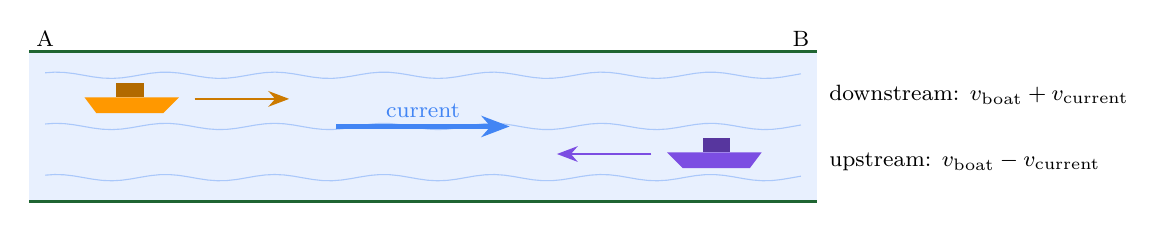
\begin{tikzpicture}[font=\footnotesize,>=Stealth]
\fill[tmBlue!12] (0,0) rectangle (10,1.9);
\draw[line width=1.2pt,tmGreen!60!black] (0,0)--(10,0) (0,1.9)--(10,1.9);
\foreach \y in {0.3,0.95,1.6}{\draw[tmBlue!45,domain=0.2:9.8,samples=80] plot (\x,{\y+0.04*sin(\x*260)});}
\draw[->,line width=1.6pt,tmBlue] (3.9,0.95)--(6.1,0.95) node[midway,above=1pt,lbl,text=tmBlue]{current};
\fill[tmOrange] (0.7,1.32)--(1.9,1.32)--(1.7,1.12)--(0.85,1.12)--cycle; \fill[tmOrange!70!black] (1.1,1.32) rectangle (1.45,1.5);
\draw[->,line width=1pt,tmOrange!80!black] (2.1,1.3)--(3.3,1.3);
\fill[tmPurple] (9.3,0.62)--(8.1,0.62)--(8.3,0.42)--(9.15,0.42)--cycle; \fill[tmPurple!70!black] (8.55,0.62) rectangle (8.9,0.8);
\draw[->,line width=1pt,tmPurple] (7.9,0.6)--(6.7,0.6);
\node[lbl,above] at (0.2,1.9){A}; \node[lbl,above] at (9.8,1.9){B};
\node[lbl,anchor=west] at (10.1,1.35){downstream: $v_{\text{boat}}+v_{\text{current}}$};
\node[lbl,anchor=west] at (10.1,0.5){upstream: $v_{\text{boat}}-v_{\text{current}}$};
\end{tikzpicture}
\end{center}
\textbf{Note:} when the same stretch AB is travelled both ways, the times are in the \emph{inverse} ratio of the speeds: the faster trip takes less time.
\end{knowbox}
\gap
\shead{Trains: moving objects that have a length}
\begin{knowbox}
A train is long, so ``the train has passed'' something only when its \emph{tail} has gone by. We follow the \emph{head} of the train and ask how far it travels.\par\smallskip
\textbf{a) Passing a pole} (a tree, a person standing still): from the moment the head reaches the pole until the tail leaves it, the head travels \emph{one train length}.
\[\text{time to pass a pole}=\text{train length}:\text{train speed}.\]
\begin{center}
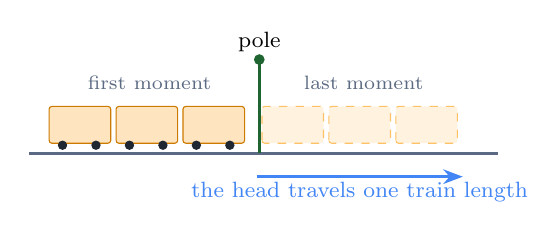
\begin{tikzpicture}[font=\footnotesize,>=Stealth,x=0.85cm,y=0.85cm]
\draw[line width=1pt,Slate] (-3.4,0)--(3.6,0);
\foreach \i in {0,1,2}{\draw[fill=tmOrange!25,draw=tmOrange!80!black,rounded corners=1pt] (-3.1+\i,0.15) rectangle ++(0.92,0.55); \fill[Ink] (-2.9+\i,0.12) circle(0.07) (-2.4+\i,0.12) circle(0.07);}
\draw[line width=1.2pt,tmGreen!60!black] (0.04,0)--(0.04,1.4); \fill[tmGreen!60!black] (0.04,1.4) circle(0.08);
\foreach \i in {0,1,2}{\draw[fill=tmOrange!12,draw=tmOrange!60,dashed,rounded corners=1pt] (0.08+\i,0.15) rectangle ++(0.92,0.55);}
\node[lbl,above] at (0.04,1.45){pole};
\node[dim] at (-1.6,1.05){first moment}; \node[dim] at (1.6,1.05){last moment};
\draw[->,tmBlue,line width=0.9pt] (0,-0.35)--node[below,lbl,text=tmBlue]{the head travels one train length}(3.08,-0.35);
\end{tikzpicture}
\end{center}
\textbf{b) Crossing a bridge} (or a tunnel, a platform): from the moment the head reaches the bridge until the tail leaves it, the head travels the \emph{bridge length plus the train length}.
\[\text{time to cross a bridge}=(\text{train length}+\text{bridge length}):\text{train speed}.\]
\begin{center}
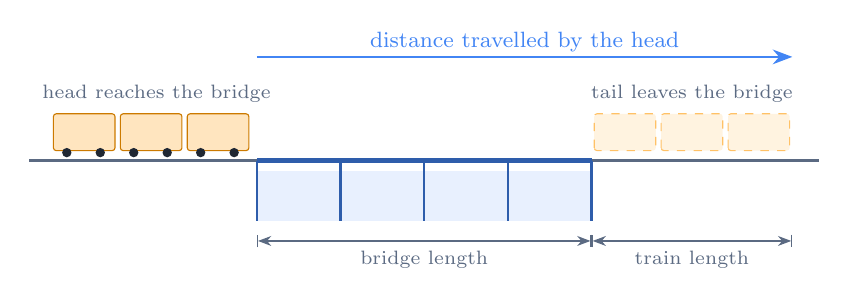
\begin{tikzpicture}[font=\footnotesize,>=Stealth,x=0.85cm,y=0.85cm]
\fill[tmBlue!12] (0,-0.9) rectangle (5,-0.15);
\draw[line width=1.2pt,Slate] (-3.4,0)--(8.4,0);
\draw[line width=2pt,tmBlue!70!black] (0,0)--(5,0); \foreach \x in {0,1.25,...,5}{\draw[tmBlue!70!black,line width=0.8pt] (\x,0)--(\x,-0.9);}
\foreach \i in {0,1,2}{\draw[fill=tmOrange!25,draw=tmOrange!80!black,rounded corners=1pt] (-3.04+\i,0.15) rectangle ++(0.92,0.55); \fill[Ink] (-2.84+\i,0.12) circle(0.07) (-2.34+\i,0.12) circle(0.07);}
\foreach \i in {0,1,2}{\draw[fill=tmOrange!12,draw=tmOrange!60,dashed,rounded corners=1pt] (5.04+\i,0.15) rectangle ++(0.92,0.55);}
\node[dim] at (-1.5,1.0){head reaches the bridge}; \node[dim] at (6.5,1.0){tail leaves the bridge};
\draw[|<->|,Slate] (0,-1.2)--node[below,dim]{bridge length}(5,-1.2);
\draw[|<->|,Slate] (5,-1.2)--node[below,dim]{train length}(8,-1.2);
\draw[->,tmBlue,line width=0.9pt] (0,1.55)--node[above,lbl,text=tmBlue]{distance travelled by the head}(8,1.55);
\end{tikzpicture}
\end{center}
\textbf{Units:} $1$ m/s $=3.6$ km/h. For example $54$ km/h $=54\,000$ m $:3\,600$ s $=15$ m/s.
\end{knowbox}
\gap
\shead{A train and another moving object}
\begin{knowbox}\begin{itemize}[leftmargin=1.4em,itemsep=3pt]
\item \textbf{Two trains in opposite directions} (on parallel tracks): from ``the heads meet'' to ``the tails part'', together they cover the sum of the two lengths.
\[\text{time}=(\text{length}_1+\text{length}_2):(v_1+v_2).\]
\item \textbf{One train overtaking another} (same direction): the faster train must gain the sum of the two lengths.
\[\text{time}=(\text{length}_1+\text{length}_2):(v_1-v_2).\]
\item \textbf{A train and a cyclist, walker or car} (a short object, its length ignored): replace the sum of the lengths by the train length only;
opposite directions: $\text{time}=\text{train length}:(v_{\text{train}}+v)$; same direction: $\text{time}=\text{train length}:(v_{\text{train}}-v)$.
\item A passenger \emph{sitting} in one train who watches another train go past sees only the length of the \emph{other} train.
\end{itemize}\end{knowbox}
\gap
\begin{exbox}{\ExWord\ 1}
The river stretch AB is $36$ km long and the current flows from A to B at $3$ km/h. At $6$:$30$ a boat whose speed in still water is $15$ km/h leaves A for B, rests $30$ minutes at B and then returns to A. At what time does it get back to A?
\guide
Downstream speed: $15+3=18$ (km/h); time from A to B: $36:18=2$ (h).\par
Upstream speed: $15-3=12$ (km/h); time from B to A: $36:12=3$ (h).\par
Back at A: $6$ h $30$ min $+\,2$ h $+\,30$ min $+\,3$ h $=12$ h $00$ min.
\dapso{at $12$:$00$ (noon).}
\end{exbox}
\gap
\begin{exbox}{\ExWord\ 2}
A canoe goes downstream from A to B in $4$ hours and comes back upstream from B to A in $6$ hours. How long does a raft take to drift from A to B?
\guide
\textit{Method 1 (choose a length).} Let AB be $12$ equal units ($12$ is divisible by both $4$ and $6$).\par
Downstream speed: $12:4=3$ (units per hour); upstream speed: $12:6=2$ (units per hour).\par
Speed of the current (= speed of the raft): $(3-2):2=0.5$ (units per hour).\par
Time for the raft: $12:0.5=24$ (h).\par\smallskip
\textit{Method 2 (fractions of AB).} In $1$ hour the canoe covers $\dfrac14$ of AB downstream and $\dfrac16$ of AB upstream.\par
In $1$ hour the current carries the raft $\left(\dfrac14-\dfrac16\right):2=\dfrac1{24}$ of AB, so the raft needs $24$ hours.
\dapso{$24$ hours.}
\end{exbox}
\gap
\begin{exbox}{\ExWord\ 3}
A train travelling at $54$ km/h passes an electricity pole in $8$ seconds.
\begin{cols2}
\pa{a} How long is the train? & \pa{b} At the same speed, how long does it take to cross a bridge $330$ m long?
\end{cols2}
\guide
$54$ km/h $=54\,000$ m $:3\,600$ s $=15$ m/s.\par
\pa{a} Passing the pole, the train travels its own length: $15\times8=120$ (m).\par
\pa{b} Crossing the bridge, it travels $120+330=450$ (m); time: $450:15=30$ (s).
\dapso{\pa{a} $120$ m;\quad \pa{b} $30$ seconds.}
\end{exbox}
\gap
\begin{exbox}{\ExWord\ 4}
Train P is $160$ m long and runs at $20$ m/s. Train Q is $140$ m long and runs at $10$ m/s on a parallel track. How long does it take them to pass each other
\begin{cols2}
\pa{a} if they run in opposite directions? & \pa{b} if P overtakes Q (same direction)?
\end{cols2}
\guide
In both cases the distance to be covered is the sum of the lengths: $160+140=300$ (m).\par
\pa{a} Opposite directions: they close up $20+10=30$ m each second; time: $300:30=10$ (s).\par
\pa{b} Same direction: P gains $20-10=10$ m each second; time: $300:10=30$ (s).
\dapso{\pa{a} $10$ seconds;\quad \pa{b} $30$ seconds.}
\end{exbox}
\gap
\begin{exbox}{\ExWord\ 5}
A train $150$ m long crosses a bridge $210$ m long in $24$ seconds. The same train overtakes a cyclist riding in the same direction in $12$ seconds. Find the cyclist's speed.
\guide
Speed of the train: $(150+210):24=15$ (m/s).\par\smallskip
\textit{Method 1.} In $12$ s the head of the train travels $15\times12=180$ (m). It started level with the cyclist and finished one train length ahead, so the cyclist rode $180-150=30$ (m).\par
Cyclist's speed: $30:12=2.5$ (m/s).\par\smallskip
\textit{Method 2.} The train gains $150$ m in $12$ s, so the difference of the speeds is $150:12=12.5$ (m/s).\par
Cyclist's speed: $15-12.5=2.5$ (m/s) $=9$ km/h.
\dapso{$2.5$ m/s (that is, $9$ km/h).}
\end{exbox}
\dividerbar{Practice}
\begin{probbox}{1}{\relax}
A boat's speed in still water is $16$ km/h and the current flows at $2$ km/h. Find the boat's speed downstream and its speed upstream.
\end{probbox}
\probsol{
Downstream: $16+2=18$ (km/h).\par Upstream: $16-2=14$ (km/h).
\dapso{$18$ km/h downstream, $14$ km/h upstream.}}
\gap
\begin{probbox}{2}{\relax}
At $7$:$15$ a boat leaves A and goes downstream, arriving at B at $9$:$45$. Its speed in still water is $21$ km/h and the current is $3$ km/h. How long is the river stretch AB?
\end{probbox}
\probsol{
Travelling time: $9$ h $45$ min $-\,7$ h $15$ min $=2$ h $30$ min $=2.5$ h.\par
Downstream speed: $21+3=24$ (km/h).\par AB: $24\times2.5=60$ (km).
\dapso{$60$ km.}}
\gap
\begin{probbox}{3}{\relax}
A canoe goes $45$ km downstream in $1$ hour $30$ minutes and comes back the same $45$ km upstream in $2$ hours $15$ minutes. Find the speed of the canoe in still water and the speed of the current.
\end{probbox}
\probsol{
$1$ h $30$ min $=1.5$ h; $2$ h $15$ min $=2.25$ h.\par
Downstream speed: $45:1.5=30$ (km/h); upstream speed: $45:2.25=20$ (km/h).\par
Still water: $(30+20):2=25$ (km/h); current: $(30-20):2=5$ (km/h).
\dapso{$25$ km/h and $5$ km/h.}}
\gap
\begin{probbox}{4}{\relax}
A canoe goes downstream from A to B, a distance of $48$ km, in $3$ hours, and back upstream in $4$ hours. How long does a leaf take to float from A to B?
\end{probbox}
\probsol{
Downstream speed: $48:3=16$ (km/h); upstream speed: $48:4=12$ (km/h).\par
Current (= the leaf's speed): $(16-12):2=2$ (km/h).\par Time for the leaf: $48:2=24$ (h).
\dapso{$24$ hours.}}
\gap
\begin{probbox}{5}{\relax}
A ferry goes downstream at $22$ km/h and upstream at $16$ km/h. Find its speed in still water and the speed of the current.
\end{probbox}
\probsol{
Still water: $(22+16):2=19$ (km/h).\par Current: $(22-16):2=3$ (km/h).
\dapso{$19$ km/h and $3$ km/h.}}
\gap
\begin{probbox}{6}{\relax}
A boat's speed in still water is $12$ km/h and the current flows at $2.5$ km/h. How long does the boat take to go $38$ km upstream?
\end{probbox}
\probsol{
Upstream speed: $12-2.5=9.5$ (km/h).\par Time: $38:9.5=4$ (h).
\dapso{$4$ hours.}}
\gap
\begin{probbox}{7}{\relax}
A boat with speed $18$ km/h in still water goes downstream from A to B in $2$ hours. The current is $3$ km/h. How long does it take to come back from B to A?
\end{probbox}
\probsol{
Downstream speed: $18+3=21$ (km/h); AB: $21\times2=42$ (km).\par
Upstream speed: $18-3=15$ (km/h); time: $42:15=2.8$ (h) $=2$ h $48$ min.
\dapso{$2$ hours $48$ minutes.}}
\gap
\begin{probbox}{8}{\relax}
A raft drifts $7.5$ km in $2.5$ hours on a river. On the same river a boat whose speed in still water is $15$ km/h goes $36$ km upstream. How long does the boat take?
\end{probbox}
\probsol{
Current: $7.5:2.5=3$ (km/h).\par Upstream speed of the boat: $15-3=12$ (km/h).\par Time: $36:12=3$ (h).
\dapso{$3$ hours.}}
\gap
\begin{probbox}{9}{\relax}
A motorboat with speed $20$ km/h in still water goes downstream from A to B and immediately comes back to A. AB is $48$ km and the current is $4$ km/h. How long is the whole trip?
\end{probbox}
\probsol{
Downstream: $48:(20+4)=2$ (h).\par Upstream: $48:(20-4)=3$ (h).\par Whole trip: $2+3=5$ (h).
\dapso{$5$ hours.}}
\gap
\begin{probbox}{10}{\relax}
A boat's downstream speed is $1.5$ times its upstream speed. The current flows at $2$ km/h. Find the speed of the boat in still water.
\end{probbox}
\probsol{
Downstream speed $-$ upstream speed $=2\times2=4$ (km/h).\par
Upstream speed $1$ part, downstream speed $1.5$ parts; the difference $0.5$ part is $4$ km/h.\par
Upstream speed: $4:0.5=8$ (km/h); downstream speed: $8\times1.5=12$ (km/h).\par
Still water: $(12+8):2=10$ (km/h).
\dapso{$10$ km/h.}}
\gap
\begin{probbox}{11}{\relax}
A boat goes downstream from A to B in $3$ hours and back upstream in $4$ hours. The current is $2$ km/h. How long is AB?
\end{probbox}
\probsol{
Same distance, so the speeds are in the inverse ratio of the times: downstream $:$ upstream $=4:3$.\par
Their difference is $2\times2=4$ (km/h), matching $4-3=1$ part.\par
Downstream speed: $4\times4=16$ (km/h); AB: $16\times3=48$ (km).
\dapso{$48$ km.}}
\gap
\begin{probbox}{12}{\relax}
A canoe goes downstream from C to D in $2$ hours and back upstream in $3$ hours. The current is $2.5$ km/h. Find the speed of the canoe in still water.
\end{probbox}
\probsol{
Downstream $:$ upstream speed $=3:2$; the difference $2\times2.5=5$ (km/h) is $1$ part.\par
Downstream speed: $15$ km/h; upstream speed: $10$ km/h.\par Still water: $(15+10):2=12.5$ (km/h).
\dapso{$12.5$ km/h.}}
\gap
\begin{probbox}{13}{\relax}
A barge takes $5$ hours to go downstream from A to B and $7$ hours to go back. How long does a log take to drift from A to B?
\end{probbox}
\probsol{
In $1$ hour the barge covers $\dfrac15$ of AB downstream and $\dfrac17$ of AB upstream.\par
In $1$ hour the current carries the log $\left(\dfrac15-\dfrac17\right):2=\dfrac2{35}:2=\dfrac1{35}$ of AB.\par So the log needs $35$ hours.
\dapso{$35$ hours.}}
\gap
\begin{probbox}{14}{\relax}
A boat with speed $15$ km/h in still water goes downstream from A to B and at once returns to A. The current is $3$ km/h and the whole trip takes $5$ hours. How long is AB?
\end{probbox}
\probsol{
Downstream speed $18$ km/h, upstream speed $12$ km/h.\par
Times are in the inverse ratio: downstream $:$ upstream $=12:18=2:3$; $5$ parts $=5$ h, so $1$ part $=1$ h.\par
Downstream time $2$ h; AB: $18\times2=36$ (km). (\emph{Check:} $36:12=3$ h upstream.)
\dapso{$36$ km.}}
\gap
\begin{probbox}{15}{\relax}
Nam rows at $4$ km/h in still water. On a river with a current of $1$ km/h he rows $6$ km upstream and then rows back to the start. How long does he take altogether?
\end{probbox}
\probsol{
Upstream: $6:(4-1)=2$ (h).\par Downstream: $6:(4+1)=1.2$ (h).\par Altogether: $3.2$ h $=3$ h $12$ min.
\dapso{$3$ hours $12$ minutes.}}
\gap
\begin{probbox}{16}{\relax}
A train travelling at $72$ km/h passes a pole in $9$ seconds. How long is the train?
\end{probbox}
\probsol{
$72$ km/h $=72\,000$ m $:3\,600$ s $=20$ m/s.\par Train length: $20\times9=180$ (m).
\dapso{$180$ m.}}
\gap
\begin{probbox}{17}{\relax}
A train $240$ m long goes past a man standing beside the track in $16$ seconds. Find its speed in m/s and in km/h.
\end{probbox}
\probsol{
Speed: $240:16=15$ (m/s).\par $15$ m/s $=15\times3.6=54$ km/h.
\dapso{$15$ m/s $=54$ km/h.}}
\gap
\begin{probbox}{18}{\relax}
A train $150$ m long runs at $15$ m/s. How long does it take to cross a bridge $300$ m long?
\end{probbox}
\probsol{
Distance travelled by the head: $150+300=450$ (m).\par Time: $450:15=30$ (s).
\dapso{$30$ seconds.}}
\gap
\begin{probbox}{19}{\relax}
A train running at $54$ km/h crosses a bridge $0.6$ km long in $48$ seconds. How long is the train?
\end{probbox}
\probsol{
$54$ km/h $=15$ m/s; $0.6$ km $=600$ m.\par Distance in $48$ s: $15\times48=720$ (m).\par Train length: $720-600=120$ (m).
\dapso{$120$ m.}}
\gap
\begin{probbox}{20}{\relax}
A train passes a pole in $10$ seconds and crosses a bridge $360$ m long in $34$ seconds. Find the speed and the length of the train.
\end{probbox}
\probsol{
The extra $34-10=24$ (s) is the time to travel the bridge length $360$ m.\par
Speed: $360:24=15$ (m/s).\par Length: $15\times10=150$ (m).
\dapso{$15$ m/s and $150$ m.}}
\gap
\begin{probbox}{21}{\relax}
A train $200$ m long runs at $20$ m/s through a tunnel $1$ km long.
\begin{cols2}
\pa{a} How long is it from the moment the head enters the tunnel until the tail leaves it? & \pa{b} For how long is the whole train inside the tunnel?
\end{cols2}
\end{probbox}
\probsol{
$1$ km $=1\,000$ m.\par
\pa{a} The head travels $1\,000+200=1\,200$ (m): $1\,200:20=60$ (s).\par
\pa{b} The whole train is inside from ``tail enters'' to ``head leaves''; the head travels $1\,000-200=800$ (m): $800:20=40$ (s).
\dapso{\pa{a} $60$ s;\quad \pa{b} $40$ s.}}
\gap
\begin{probbox}{22}{\relax}
A train $180$ m long passes a cyclist riding towards it at $18$ km/h in $9$ seconds. Find the speed of the train in km/h.
\end{probbox}
\probsol{
$18$ km/h $=5$ m/s.\par Sum of the speeds: $180:9=20$ (m/s).\par
Train: $20-5=15$ (m/s) $=54$ km/h.
\dapso{$54$ km/h.}}
\gap
\begin{probbox}{23}{\relax}
A train $200$ m long overtakes a jogger running at $2$ m/s in the same direction. It takes $25$ seconds. Find the speed of the train in km/h.
\end{probbox}
\probsol{
Difference of the speeds: $200:25=8$ (m/s).\par Train: $8+2=10$ (m/s) $=36$ km/h.
\dapso{$36$ km/h.}}
\gap
\begin{probbox}{24}{\relax}
A train $120$ m long at $54$ km/h meets a train $180$ m long at $36$ km/h coming the other way on a parallel track. How long do they take to pass each other?
\end{probbox}
\probsol{
$54$ km/h $=15$ m/s; $36$ km/h $=10$ m/s.\par Sum of lengths: $300$ m; sum of speeds: $25$ m/s.\par Time: $300:25=12$ (s).
\dapso{$12$ seconds.}}
\gap
\begin{probbox}{25}{\relax}
An express train $160$ m long at $20$ m/s overtakes a goods train $140$ m long at $15$ m/s on a parallel track. How long does the overtaking take?
\end{probbox}
\probsol{
Sum of lengths: $160+140=300$ (m).\par Difference of speeds: $20-15=5$ (m/s).\par Time: $300:5=60$ (s) $=1$ min.
\dapso{$1$ minute.}}
\gap
\begin{probbox}{26}{\relax}
A car at $72$ km/h drives alongside a train going the same way at $54$ km/h. It takes the car $40$ seconds to get from the tail to the head of the train. How long is the train?
\end{probbox}
\probsol{
$72$ km/h $=20$ m/s; $54$ km/h $=15$ m/s.\par The car gains $20-15=5$ m each second.\par Train length: $5\times40=200$ (m).
\dapso{$200$ m.}}
\gap
\begin{probbox}{27}{\relax}
Lan sits by the window of a train running at $15$ m/s. A train on the next track, running the other way at $10$ m/s, takes $9$ seconds to go past her window. How long is that train?
\end{probbox}
\probsol{
Lan sees only the other train's length go by, at $15+10=25$ (m/s).\par Length: $25\times9=225$ (m).
\dapso{$225$ m.}}
\gap
\begin{probbox}{28}{\relax}
A train passes a signal post in $10$ seconds and passes along a platform $150$ m long in $16$ seconds. Find the length and the speed of the train.
\end{probbox}
\probsol{
The platform needs $16-10=6$ (s) more, so the speed is $150:6=25$ (m/s).\par Length: $25\times10=250$ (m).
\dapso{$250$ m and $25$ m/s.}}
\gap
\begin{probbox}{29}{\relax}
A train $150$ m long runs at $15$ m/s and crosses a bridge in $40$ seconds. How long is the bridge?
\end{probbox}
\probsol{
Distance travelled: $15\times40=600$ (m).\par Bridge: $600-150=450$ (m).
\dapso{$450$ m.}}
\gap
\begin{probbox}{30}{\relax}
A train crosses a bridge $240$ m long in $25$ seconds and a bridge $420$ m long in $37$ seconds, at the same speed. Find the speed and the length of the train.
\end{probbox}
\probsol{
The second bridge is $420-240=180$ (m) longer and takes $37-25=12$ (s) longer.\par
Speed: $180:12=15$ (m/s).\par Distance for the first bridge: $15\times25=375$ (m); train: $375-240=135$ (m).
\dapso{$15$ m/s and $135$ m.}}
\dividerbar{Challenge -- Extension}
\begin{probbox}{31}{\stars{1}}
A boat with speed $18$ km/h in still water goes downstream from A to B and at once comes back. The current is $2$ km/h and the round trip takes $4$ hours $30$ minutes. How long is AB?
\end{probbox}
\probsol{
Downstream speed $20$ km/h, upstream speed $16$ km/h.\par
Times: downstream $:$ upstream $=16:20=4:5$.\par $9$ parts $=4.5$ h, so $1$ part $=0.5$ h; downstream time $2$ h.\par
AB: $20\times2=40$ (km).
\dapso{$40$ km.}}
\gap
\begin{probbox}{32}{\stars{1}}
Ports A and B are $60$ km apart and the river flows from A to B at $3$ km/h. At the same moment a boat leaves A for B and another boat leaves B for A; both have speed $20$ km/h in still water. After how long do they meet, and how far from A?
\end{probbox}
\probsol{
Speeds: $20+3=23$ (km/h) and $20-3=17$ (km/h).\par
Sum: $23+17=40$ (km/h) (the current helps one boat as much as it slows the other).\par
Time: $60:40=1.5$ (h); distance from A: $23\times1.5=34.5$ (km).
\dapso{after $1$ h $30$ min, $34.5$ km from A.}}
\gap
\begin{probbox}{33}{\stars{2}}
As a boat leaves A downstream, a raft is let go at A. The boat ($12$ km/h in still water, current $3$ km/h) reaches B, $30$ km from A, and immediately turns back. How long after leaving A does it meet the raft?
\end{probbox}
\probsol{
Boat downstream: $30:15=2$ (h). Meanwhile the raft drifts $3\times2=6$ (km).\par
Gap when the boat turns: $30-6=24$ (km). The boat goes up at $9$ km/h, the raft comes down at $3$ km/h: they close $12$ km each hour.\par
They meet after $24:12=2$ (h) more, i.e.\ $2+2=4$ (h) after leaving A.
\note{Seen from the water, the boat moves away from the raft for $2$ h and comes back for $2$ h: the current does not matter.}
\dapso{$4$ hours.}}
\gap
\begin{probbox}{34}{\stars{2}}
Rowing upstream, Bình's hat falls into the water. He notices $20$ minutes later, turns round at once and picks up his hat $2$ km downstream of the place where it fell. Find the speed of the current.
\end{probbox}
\probsol{
Relative to the water, the hat stays still and Bình rows away from it for $20$ minutes, so he also needs $20$ minutes to come back to it.\par
So the hat drifted for $20+20=40$ (min) $=\dfrac23$ h, travelling $2$ km.\par
Current: $2:\dfrac23=3$ (km/h).
\dapso{$3$ km/h.}}
\gap
\begin{probbox}{35}{\stars{1}}
A ferry goes downstream at $20$ km/h and upstream at $12$ km/h. It goes from A to B, rests $30$ minutes at B and comes back; the whole trip takes $4$ hours $30$ minutes. How long is AB?
\end{probbox}
\probsol{
Moving time: $4$ h $30$ min $-\,30$ min $=4$ h.\par
Times: downstream $:$ upstream $=12:20=3:5$; $8$ parts $=4$ h, $1$ part $=0.5$ h.\par
Downstream time $1.5$ h; AB: $20\times1.5=30$ (km).
\dapso{$30$ km.}}
\gap
\begin{probbox}{36}{\stars{1}}
A boat's speed in still water is $4$ times the speed of the current. It goes downstream from A to B in $2$ hours. How long does it take to go back?
\end{probbox}
\probsol{
Let the current be $1$ part: still water $4$ parts, downstream $5$ parts, upstream $3$ parts.\par
Times are in the inverse ratio: upstream time $=2\times5:3=\dfrac{10}3$ (h) $=3$ h $20$ min.
\dapso{$3$ hours $20$ minutes.}}
\gap
\begin{probbox}{37}{\stars{1}}
A canoe goes downstream from A to B in $3$ hours and back in $4$ hours $30$ minutes. If its engine were switched off, how long would it take to drift from A to B?
\end{probbox}
\probsol{
In $1$ hour: downstream $\dfrac13$ of AB, upstream $1:4.5=\dfrac29$ of AB.\par
The current carries the canoe $\left(\dfrac13-\dfrac29\right):2=\dfrac1{18}$ of AB per hour.\par Drifting time: $18$ hours.
\dapso{$18$ hours.}}
\gap
\begin{probbox}{38}{\stars{1}}
At $7$:$00$ a boat leaves B upstream and reaches A at $10$:$00$. It rests, leaves A at $10$:$30$ and gets back to B at $12$:$30$. The current is $2$ km/h. How far is it from A to B?
\end{probbox}
\probsol{
Upstream $3$ h, downstream $2$ h; speeds upstream $:$ downstream $=2:3$.\par
The difference $2\times2=4$ (km/h) is $1$ part; upstream speed $8$ km/h.\par AB: $8\times3=24$ (km).
\dapso{$24$ km.}}
\gap
\begin{probbox}{39}{\stars{2}}
At $6$:$00$ a raft starts drifting from A. At $8$:$00$ a boat leaves A downstream ($9$ km/h in still water). The current is $3$ km/h. At what time does the boat catch the raft, and how far from A?
\end{probbox}
\probsol{
At $8$:$00$ the raft is $3\times2=6$ (km) ahead.\par
Boat downstream $12$ km/h, raft $3$ km/h: the boat gains $9$ km/h (its still-water speed).\par
Time: $6:9=\dfrac23$ (h) $=40$ min, at $8$:$40$; distance from A: $12\times\dfrac23=8$ (km).
\dapso{at $8$:$40$, $8$ km from A.}}
\gap
\begin{probbox}{40}{\stars{2}}
A train overtakes a man walking in the same direction at $1$ m/s in $22$ seconds, and passes a man walking towards it at $1$ m/s in $18$ seconds. Find the speed and the length of the train.
\end{probbox}
\probsol{
In both cases the train covers its own length: once at speed $v-1$ (in $22$ s), once at speed $v+1$ (in $18$ s).\par
Same length, so $(v-1):(v+1)=18:22=9:11$; their difference $2$ m/s is $2$ parts, so $1$ part $=1$ m/s.\par
$v-1=9$, so $v=10$ m/s; length: $9\times22=198$ (m).
\dapso{$10$ m/s and $198$ m.}}
\gap
\begin{probbox}{41}{\stars{2}}
A train goes through a tunnel $1.5$ km long. From the moment its head enters until its tail leaves takes $90$ seconds; the whole train is inside the tunnel for $60$ seconds. Find the speed and the length of the train.
\end{probbox}
\probsol{
In $90$ s the head travels tunnel $+$ train; in $60$ s it travels tunnel $-$ train.\par
Together: in $150$ s it travels $2$ tunnels $=3\,000$ m; speed: $3\,000:150=20$ (m/s).\par
Tunnel $+$ train $=20\times90=1\,800$ (m); train: $1\,800-1\,500=300$ (m).
\dapso{$20$ m/s and $300$ m.}}
\gap
\begin{probbox}{42}{\stars{2}}
An express train $180$ m long runs at $24$ m/s. It takes $50$ seconds to overtake a slower train on a parallel track; if the two trains ran towards each other they would pass in $10$ seconds. Find the speed and the length of the slower train.
\end{probbox}
\probsol{
The same distance (the two lengths) takes $50$ s with the difference of speeds and $10$ s with the sum, so sum $:$ difference $=5:1$.\par
Sum $5$ parts, difference $1$ part: express $=3$ parts, slow $=2$ parts; $3$ parts $=24$ m/s.\par
Slow train: $16$ m/s. Two lengths: $(24+16)\times10=400$ (m); slow train: $400-180=220$ (m).
\dapso{$16$ m/s and $220$ m.}}
\gap
\begin{probbox}{43}{\stars{1}}
A passenger on a train running at $54$ km/h sees a train $300$ m long, coming the other way, go past in $12$ seconds. Find the speed of that train in km/h.
\end{probbox}
\probsol{
Sum of speeds: $300:12=25$ (m/s).\par Other train: $25-15=10$ (m/s) $=36$ km/h.
\dapso{$36$ km/h.}}
\gap
\begin{probbox}{44}{\stars{1}}
A bridge is $4$ times as long as a train. The train, at $20$ m/s, takes $25$ seconds from the moment its head reaches the bridge until its tail leaves it. Find the length of the train and of the bridge.
\end{probbox}
\probsol{
Distance: $20\times25=500$ (m) $=$ bridge $+$ train $=5$ train lengths.\par
Train: $500:5=100$ (m); bridge: $400$ m.
\dapso{train $100$ m, bridge $400$ m.}}
\gap
\begin{probbox}{45}{\stars{1}}
Two trains, each $150$ m long, pass each other going in opposite directions in $10$ seconds. One train is $1.5$ times as fast as the other. Find their speeds.
\end{probbox}
\probsol{
Sum of speeds: $300:10=30$ (m/s).\par Slower $1$ part, faster $1.5$ parts: $30:2.5=12$ (m/s).\par Faster: $18$ m/s.
\dapso{$12$ m/s and $18$ m/s.}}
\gap
\begin{probbox}{46}{\stars{1}}
Train A, $240$ m long, at $72$ km/h overtakes train B going the same way at $54$ km/h. The overtaking takes $1$ minute $30$ seconds. How long is train B?
\end{probbox}
\probsol{
Difference of speeds: $20-15=5$ (m/s); $1$ min $30$ s $=90$ s.\par Sum of lengths: $5\times90=450$ (m).\par Train B: $450-240=210$ (m).
\dapso{$210$ m.}}
\gap
\begin{probbox}{47}{\stars{2}}
On a river with a current of $1$ m/s, a cargo ship $80$ m long sails downstream ($6$ m/s in still water) and meets a ship $70$ m long sailing upstream ($4$ m/s in still water). How long do they take to pass each other?
\end{probbox}
\probsol{
Speeds: $6+1=7$ (m/s) and $4-1=3$ (m/s); sum $10$ m/s (equal to the sum of the still-water speeds).\par
Sum of lengths: $150$ m. Time: $150:10=15$ (s).
\dapso{$15$ seconds.}}
\gap
\begin{probbox}{48}{\stars{2}}
A line of pupils $300$ m long walks at $1.5$ m/s. A cyclist rides at $4.5$ m/s from the back of the line to the front and immediately back to the end. How long does this take?
\end{probbox}
\probsol{
Back to front (same direction): he gains $4.5-1.5=3$ (m/s): $300:3=100$ (s).\par
Front to back (towards the line): $4.5+1.5=6$ (m/s): $300:6=50$ (s).\par Total: $150$ s $=2$ min $30$ s.
\dapso{$2$ minutes $30$ seconds.}}
\gap
\begin{probbox}{49}{\stars{1}}
A train $250$ m long runs at $72$ km/h. Its head enters a tunnel at $9$:$00$:$00$ and its tail leaves at $9$:$01$:$40$. How long is the tunnel?
\end{probbox}
\probsol{
Time: $1$ min $40$ s $=100$ s; speed $20$ m/s.\par Distance: $20\times100=2\,000$ (m).\par Tunnel: $2\,000-250=1\,750$ (m).
\dapso{$1\,750$ m.}}
\gap
\begin{probbox}{50}{\stars{2}}
A boat's upstream speed is $\dfrac23$ of its downstream speed. A raft drifts from A to B in $30$ hours. How long does the boat take from A to B downstream, and from B to A upstream?
\end{probbox}
\probsol{
Downstream $3$ parts, upstream $2$ parts; difference $1$ part $=2\times$ current, so the current is $\dfrac12$ part.\par
Downstream speed is $3:\dfrac12=6$ times the current: $30:6=5$ (h).\par
Upstream speed is $4$ times the current: $30:4=7.5$ (h) $=7$ h $30$ min.
\dapso{$5$ hours downstream, $7$ hours $30$ minutes upstream.}}
\clearpage
\titlehead
\begingroup\setbox0=\vbox{\section*{Motion around a Circular Track}}\endgroup
\chapterhead{10}{Motion around a Circular Track}
\shead{Moving round a closed track}
\begin{knowbox}\begin{itemize}[leftmargin=1.4em,itemsep=3pt]
\item Runners on a running track, cyclists round a lake, the hands of a clock\ldots\ all move round a closed path. After each full lap the mover is back exactly where it started, and it can go round as many times as it likes.
\item If one lap is $C$ and the distance travelled is $s$, then $s:C$ gives the number of whole laps, and the remainder tells us how far past the start the mover is.
For a circular track, $C=\text{diameter}\times3.14$.
\item \textbf{Careful:} ``how far from the start'' along the way ahead is \emph{one lap minus the remainder}, not the remainder itself.
\end{itemize}\end{knowbox}
\gap
\shead{Two movers starting together from the same point}
\begin{knowbox}
\begin{center}
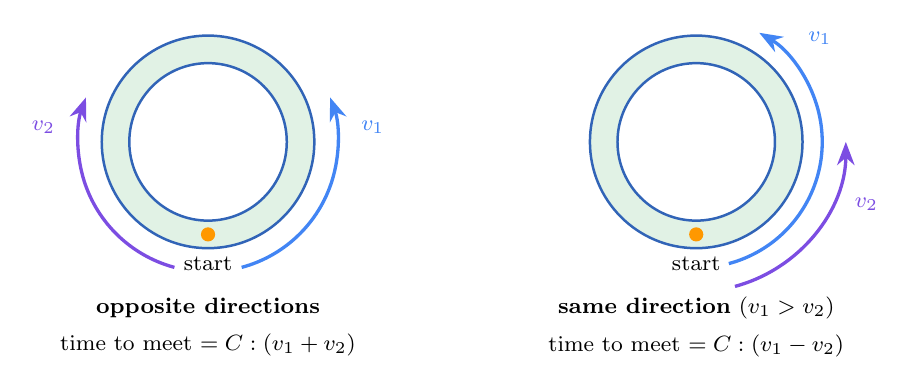
\begin{tikzpicture}[>=Stealth,font=\footnotesize]
\begin{scope}
\fill[tmGreen!15,even odd rule] (0,0) circle(1.35) (0,0) circle(1.0);
\draw[geo] (0,0) circle(1.35) (0,0) circle(1.0);
\fill[tmOrange] (0,-1.175) circle(0.09); \node[lbl,below] at (0,-1.4){start};
\draw[->,tmBlue,line width=1.2pt] (-75:1.65) arc(-75:20:1.65); \node[lbl,text=tmBlue] at (5:2.1){$v_1$};
\draw[->,tmPurple,line width=1.2pt] (-105:1.65) arc(-105:-200:1.65); \node[lbl,text=tmPurple] at (-185:2.1){$v_2$};
\node[lbl,align=center] at (0,-2.35){\textbf{opposite directions}\\ time to meet $=C:(v_1+v_2)$};
\end{scope}
\begin{scope}[xshift=6.2cm]
\fill[tmGreen!15,even odd rule] (0,0) circle(1.35) (0,0) circle(1.0);
\draw[geo] (0,0) circle(1.35) (0,0) circle(1.0);
\fill[tmOrange] (0,-1.175) circle(0.09); \node[lbl,below] at (0,-1.4){start};
\draw[->,tmBlue,line width=1.2pt] (-75:1.6) arc(-75:60:1.6); \node[lbl,text=tmBlue] at (40:2.05){$v_1$};
\draw[->,tmPurple,line width=1.2pt] (-75:1.9) arc(-75:0:1.9); \node[lbl,text=tmPurple] at (-20:2.3){$v_2$};
\node[lbl,align=center] at (0,-2.35){\textbf{same direction} ($v_1>v_2$)\\ time to meet $=C:(v_1-v_2)$};
\end{scope}
\end{tikzpicture}
\end{center}
\begin{itemize}[leftmargin=1.4em,itemsep=3pt]
\item \textbf{Opposite directions:} they meet each time that together they have covered one lap.
\item \textbf{Same direction:} they meet each time the faster one has gained one whole lap on the slower one (it ``laps'' the slower one).
\item After the first meeting the situation repeats: the 2nd, 3rd, \ldots\ meetings come after $2,\ 3,\ \ldots$ times that time.
\item If they do not start together, use the gap between them in place of $C$ for the first meeting.
\end{itemize}
\textbf{Clock hands} move round the clock face, which has $60$ minute-divisions: the minute hand moves $1$ division per minute and the hour hand $\dfrac1{12}$ division per minute.
\end{knowbox}
\gap
\shead{Going back and forth on a road}
\begin{knowbox}
Two people start at the same time from the two ends A and B of a road, walk towards each other, and each turns back at once on reaching the other end.
\begin{center}
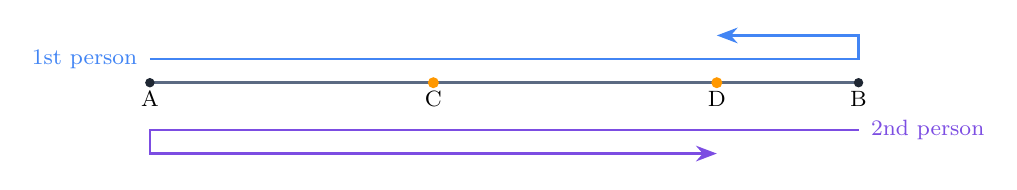
\begin{tikzpicture}[>=Stealth,font=\footnotesize]
\draw[line width=1.2pt,Slate] (0,0)--(9,0);
\foreach \x/\n in {0/A,9/B}{\fill[Ink] (\x,0) circle(0.06); \node[lbl,below] at (\x,-0.05){\n};}
\fill[tmOrange] (3.6,0) circle(0.07); \node[lbl,below] at (3.6,-0.05){C};
\fill[tmOrange] (7.2,0) circle(0.07); \node[lbl,below] at (7.2,-0.05){D};
\draw[->,tmBlue,line width=1pt] (0,0.3)--(9,0.3)--(9,0.6)--(7.2,0.6);
\draw[->,tmPurple,line width=1pt] (9,-0.6)--(0,-0.6)--(0,-0.9)--(7.2,-0.9);
\node[lbl,text=tmBlue,anchor=east] at (-0.1,0.3){1st person};
\node[lbl,text=tmPurple,anchor=west] at (9.1,-0.6){2nd person};
\end{tikzpicture}
\end{center}
\begin{itemize}[leftmargin=1.4em,itemsep=3pt]
\item By the first meeting (at C) together they have covered \emph{one} length AB.
\item By the second meeting (at D, after both have turned back) together they have covered \emph{three} lengths AB, so it takes $3$ times as long, and each person has walked $3$ times as far as before the first meeting.
\end{itemize}
\note{This holds when the faster person is less than twice as fast as the slower one, so that nobody is caught from behind before the second meeting.}
\end{knowbox}
\gap
\begin{exbox}{\ExWord\ 1}
Minh and Hà cycle round a lake whose shore path is $1.5$ km long. Minh rides at $12$ km/h and Hà at $15$ km/h. They start together from the same point and go the same way. After how long do they meet for the first time (not counting the start)?
\guide
To meet again, Hà must gain one whole lap, $1.5$ km, on Minh.\par
Difference of speeds: $15-12=3$ (km/h).\par
Time: $1.5:3=0.5$ (h) $=30$ min.
\dapso{$30$ minutes.}
\end{exbox}
\gap
\begin{exbox}{\ExWord\ 2}
On a $400$ m running track, Tú runs at $3$ m/s and Quân at $5$ m/s. They start together from the same point and run in opposite directions.
\begin{cols3}
\pa{a} After how long do they first meet? & \pa{b} How far from the start is that, along Tú's way? & \pa{c} How many times do they meet in $10$ minutes?
\end{cols3}
\guide
\pa{a} Together they cover one lap: $400:(3+5)=50$ (s).\par
\pa{b} In $50$ s Tú runs $3\times50=150$ (m): they meet $150$ m from the start along Tú's way (and $250$ m along Quân's way).\par
\pa{c} $10$ min $=600$ s; they meet every $50$ s, so $600:50=12$ times.
\dapso{\pa{a} $50$ s;\quad \pa{b} $150$ m;\quad \pa{c} $12$ times.}
\end{exbox}
\gap
\begin{exbox}{\ExWord\ 3}
Dũng jogs from his house round a block whose loop is $1.8$ km long, at $8$ km/h. After $45$ minutes, how much farther must he run, keeping the same way, to get back home?
\guide
$45$ min $=0.75$ h; distance run: $8\times0.75=6$ (km).\par
$6:1.8=3$ laps, remainder $0.6$ km ($6=3\times1.8+0.6$): Dũng is $0.6$ km past his house.\par
To get home going forward he still needs $1.8-0.6=1.2$ (km).
\note{Do not answer $0.6$ km: that is how far he has gone \emph{past} the house, not how far he still has to go.}
\dapso{$1.2$ km.}
\end{exbox}
\gap
\begin{exbox}{\ExWord\ 4}
A circular running track has diameter $100$ m. Two pupils start together from the same point and run the same way at $4.5$ m/s and $2.5$ m/s. After how long does the faster one first catch the slower one?
\guide
Length of one lap: $100\times3.14=314$ (m).\par
Difference of speeds: $4.5-2.5=2$ (m/s).\par
Time: $314:2=157$ (s) $=2$ min $37$ s.
\dapso{$2$ minutes $37$ seconds.}
\end{exbox}
\gap
\begin{exbox}{\ExWord\ 5}
Two friends set off at the same time, one from A towards B and one from B towards A. They meet first at C, $14$ km from A. Each goes on to the other end and turns back at once; they meet a second time at D, $8$ km from B. How long is the road AB?
\guide
\begin{center}
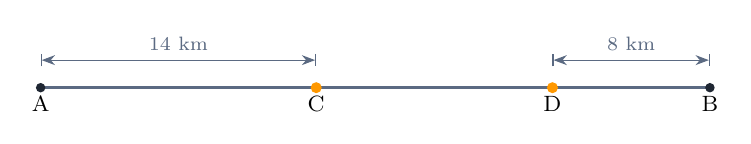
\begin{tikzpicture}[>=Stealth,font=\footnotesize]
\draw[line width=1.2pt,Slate] (0,0)--(8.5,0);
\foreach \x/\n in {0/A,8.5/B}{\fill[Ink] (\x,0) circle(0.06); \node[lbl,below] at (\x,-0.05){\n};}
\fill[tmOrange] (3.5,0) circle(0.07); \node[lbl,below] at (3.5,-0.05){C};
\fill[tmOrange] (6.5,0) circle(0.07); \node[lbl,below] at (6.5,-0.05){D};
\draw[|<->|,Slate] (0,0.35)--node[above,dim]{$14$ km}(3.5,0.35);
\draw[|<->|,Slate] (6.5,0.35)--node[above,dim]{$8$ km}(8.5,0.35);
\end{tikzpicture}
\end{center}
By the first meeting the two together have covered one AB; the friend from A has walked $14$ km.\par
By the second meeting they together have covered three AB, so the friend from A has walked $14\times3=42$ (km).\par
He walked from A to B and then $8$ km back: $42=\text{AB}+8$, so $\text{AB}=42-8=34$ (km).
\note{Check: the speeds are in the ratio $14:20$; the friend from B walks $20\times3=60=34+26$ km, i.e.\ to A and $26$ km back, which is $8$ km from B.}
\dapso{$34$ km.}
\end{exbox}
\dividerbar{Practice}
\begin{probbox}{1}{\relax}
On a $400$ m track two runners start together from the same point and run in opposite directions at $4$ m/s and $6$ m/s. After how long do they first meet?
\end{probbox}
\probsol{
Together they cover one lap.\par Sum of speeds: $4+6=10$ (m/s).\par Time: $400:10=40$ (s).
\dapso{$40$ seconds.}}
\gap
\begin{probbox}{2}{\relax}
The same two runners (at $4$ m/s and $6$ m/s) start together from the same point on the $400$ m track but run the same way. After how long do they first meet?
\end{probbox}
\probsol{
The faster runner must gain one lap.\par Difference of speeds: $6-4=2$ (m/s).\par Time: $400:2=200$ (s) $=3$ min $20$ s.
\dapso{$3$ minutes $20$ seconds.}}
\gap
\begin{probbox}{3}{\relax}
A lake path is $3$ km round. Two cyclists start together from the same point in opposite directions at $12$ km/h and $18$ km/h. After how many minutes do they meet?
\end{probbox}
\probsol{
Sum of speeds: $12+18=30$ (km/h).\par Time: $3:30=0.1$ (h) $=6$ min.
\dapso{$6$ minutes.}}
\gap
\begin{probbox}{4}{\relax}
The two cyclists of Problem 3 now ride the same way round the $3$ km lake. After how long does the faster one first catch up with the other?
\end{probbox}
\probsol{
Difference of speeds: $18-12=6$ (km/h).\par Time: $3:6=0.5$ (h) $=30$ min.
\dapso{$30$ minutes.}}
\gap
\begin{probbox}{5}{\relax}
A park path is a loop of $900$ m. Lan walks at $60$ m/min and Mai at $90$ m/min; they start together from the gate and walk the same way. After how long does Mai first catch up with Lan, and how many laps has each walked by then?
\end{probbox}
\probsol{
Difference of speeds: $90-60=30$ (m/min).\par Time: $900:30=30$ (min).\par
Lan: $60\times30=1\,800$ m $=2$ laps; Mai: $90\times30=2\,700$ m $=3$ laps.
\dapso{after $30$ minutes; Lan $2$ laps, Mai $3$ laps.}}
\gap
\begin{probbox}{6}{\relax}
An runs round an $800$ m track at $150$ m/min for $14$ minutes. How many full laps has he run, and how many more metres must he run to finish the lap he is on?
\end{probbox}
\probsol{
Distance: $150\times14=2\,100$ (m).\par $2\,100=2\times800+500$: $2$ full laps and $500$ m more.\par
To finish the third lap: $800-500=300$ (m).
\dapso{$2$ full laps; $300$ m more.}}
\gap
\begin{probbox}{7}{\relax}
A circular cycle track has diameter $50$ m. A child rides $5$ laps. How far does the child ride?
\end{probbox}
\probsol{
One lap: $50\times3.14=157$ (m).\par $5$ laps: $157\times5=785$ (m).
\dapso{$785$ m.}}
\gap
\begin{probbox}{8}{\relax}
A circular track has diameter $100$ m. Two pupils start together from the same point and run in opposite directions at $3$ m/s and $5$ m/s. After how long do they meet?
\end{probbox}
\probsol{
One lap: $100\times3.14=314$ (m).\par Sum of speeds: $3+5=8$ (m/s).\par Time: $314:8=39.25$ (s).
\dapso{$39.25$ seconds.}}
\gap
\begin{probbox}{9}{\relax}
Two cyclists ride the same way round a $2$ km circuit at $20$ km/h and $25$ km/h, starting together. How many times does the faster one overtake the slower one in $2$ hours?
\end{probbox}
\probsol{
In $2$ hours the faster one gains $(25-20)\times2=10$ (km).\par Each overtaking is a gain of one lap: $10:2=5$ (times).
\dapso{$5$ times.}}
\gap
\begin{probbox}{10}{\relax}
Two runners start together from the same point of a $500$ m track and run in opposite directions at $3$ m/s and $2$ m/s. How many times do they meet in $10$ minutes?
\end{probbox}
\probsol{
They meet every $500:(3+2)=100$ (s).\par $10$ min $=600$ s; $600:100=6$ (times).
\dapso{$6$ times.}}
\gap
\begin{probbox}{11}{\relax}
Two friends run the same way round a $1$ km loop, starting together. The faster one runs at $250$ m/min and catches the other for the first time after $10$ minutes. Find the speed of the slower one.
\end{probbox}
\probsol{
Difference of speeds: $1\,000:10=100$ (m/min).\par Slower one: $250-100=150$ (m/min).
\dapso{$150$ m/min.}}
\gap
\begin{probbox}{12}{\relax}
Two friends run in opposite directions round a $600$ m loop, starting together, and meet after $2$ minutes. One runs at $140$ m/min. Find the speed of the other.
\end{probbox}
\probsol{
Sum of speeds: $600:2=300$ (m/min).\par The other: $300-140=160$ (m/min).
\dapso{$160$ m/min.}}
\gap
\begin{probbox}{13}{\relax}
On a $400$ m track, Bảo starts $100$ m ahead of Khoa, and both run the same way. Khoa runs at $5$ m/s, Bảo at $3$ m/s. After how long does Khoa catch Bảo?
\end{probbox}
\probsol{
Khoa must gain $100$ m.\par Difference of speeds: $5-3=2$ (m/s).\par Time: $100:2=50$ (s).
\dapso{$50$ seconds.}}
\gap
\begin{probbox}{14}{\relax}
Hùng runs one lap of a track in $4$ minutes, Việt in $6$ minutes. They start together from the same point and run the same way. After how long does Hùng first catch Việt?
\end{probbox}
\probsol{
Each minute Hùng runs $\dfrac14$ lap and Việt $\dfrac16$ lap; Hùng gains $\dfrac14-\dfrac16=\dfrac1{12}$ lap.\par
To gain one lap: $1:\dfrac1{12}=12$ (min).
\dapso{$12$ minutes.}}
\gap
\begin{probbox}{15}{\relax}
Hùng and Việt (one lap in $4$ min and in $6$ min) now start together and run in opposite directions. After how long do they meet?
\end{probbox}
\probsol{
Each minute together they run $\dfrac14+\dfrac16=\dfrac5{12}$ lap.\par
Time: $1:\dfrac5{12}=\dfrac{12}5=2.4$ (min) $=2$ min $24$ s.
\dapso{$2$ minutes $24$ seconds.}}
\gap
\begin{probbox}{16}{\relax}
One runner takes $3$ minutes per lap and another $5$ minutes per lap. They start together from the start line. After how long are both at the start line together again for the first time?
\end{probbox}
\probsol{
The first runner is at the start line after $3,\ 6,\ 9,\ 12,\ 15,\ldots$ minutes; the second after $5,\ 10,\ 15,\ldots$ minutes.\par
The smallest common number: $15$.
\dapso{$15$ minutes.}}
\gap
\begin{probbox}{17}{\relax}
A runner runs $5$ laps of a $400$ m track in $10$ minutes. Find the speed in m/min and in km/h.
\end{probbox}
\probsol{
Distance: $400\times5=2\,000$ (m).\par Speed: $2\,000:10=200$ (m/min).\par $200$ m/min $=12\,000$ m/h $=12$ km/h.
\dapso{$200$ m/min $=12$ km/h.}}
\gap
\begin{probbox}{18}{\relax}
A road AB is $30$ km long. A cyclist leaves A for B at $12$ km/h, and at the same time a motorcyclist leaves B for A at $18$ km/h. Each turns back at once on reaching the other end.
\begin{cols2}
\pa{a} How far from A do they meet the first time? & \pa{b} How far from A do they meet the second time?
\end{cols2}
\end{probbox}
\probsol{
\pa{a} Time: $30:(12+18)=1$ (h); distance from A: $12\times1=12$ (km).\par
\pa{b} By the second meeting they together cover $3\times30=90$ (km), which takes $3$ h.\par
The cyclist rides $12\times3=36$ (km) $=30+6$: to B and $6$ km back, which is $30-6=24$ (km) from A.
\dapso{\pa{a} $12$ km;\quad \pa{b} $24$ km.}}
\gap
\begin{probbox}{19}{\relax}
Two people set off at the same time from A and from B towards each other. They meet first $9$ km from A. Each goes on to the other end and turns back at once; they meet again $5$ km from B. How long is AB?
\end{probbox}
\probsol{
By the second meeting the person from A has walked $9\times3=27$ (km).\par
That is AB plus $5$ km back from B: $\text{AB}=27-5=22$ (km).
\dapso{$22$ km.}}
\gap
\begin{probbox}{20}{\relax}
Hoa walks from A and Quế from B towards each other, then back and forth between A and B without stopping. Their speeds are in the ratio $2:3$. The first two meeting points are $24$ m apart. How long is AB?
\end{probbox}
\probsol{
First meeting: Hoa has walked $\dfrac25$ of AB.\par
Second meeting: Hoa has walked $3\times\dfrac25=\dfrac65$ of AB, i.e.\ to B and $\dfrac15$ AB back: she is $\dfrac45$ of AB from A.\par
Distance between the meeting points: $\dfrac45-\dfrac25=\dfrac25$ of AB $=24$ m; AB $=24:\dfrac25=60$ (m).
\dapso{$60$ m.}}
\gap
\begin{probbox}{21}{\relax}
A bicycle wheel has diameter $0.6$ m. How many turns does it make while the bicycle travels $942$ m?
\end{probbox}
\probsol{
One turn: $0.6\times3.14=1.884$ (m).\par Turns: $942:1.884=500$.
\dapso{$500$ turns.}}
\gap
\begin{probbox}{22}{\relax}
The minute hand of a clock is $10$ cm long. How far does its tip travel in $1$ hour? In $3$ hours?
\end{probbox}
\probsol{
In $1$ hour the tip goes once round a circle of radius $10$ cm: $10\times2\times3.14=62.8$ (cm).\par
In $3$ hours: $62.8\times3=188.4$ (cm).
\dapso{$62.8$ cm; $188.4$ cm.}}
\gap
\begin{probbox}{23}{\relax}
On a $400$ m track, A runs at $6$ m/s and B at $4$ m/s, the same way, starting together. When A first laps B, how many metres and how many laps has A run?
\end{probbox}
\probsol{
Time: $400:(6-4)=200$ (s).\par A runs $6\times200=1\,200$ (m) $=3$ laps.
\dapso{$1\,200$ m, $3$ laps.}}
\gap
\begin{probbox}{24}{\relax}
Phúc runs one lap of a track in $80$ seconds and Long in $120$ seconds. They start together and run in opposite directions. After how long do they meet?
\end{probbox}
\probsol{
Each second together they run $\dfrac1{80}+\dfrac1{120}=\dfrac3{240}+\dfrac2{240}=\dfrac1{48}$ lap.\par Time: $48$ s.
\dapso{$48$ seconds.}}
\gap
\begin{probbox}{25}{\relax}
Two horses gallop the same way round a $1.2$ km racecourse at $15$ m/s and $12$ m/s, starting together. After how long does the faster one first catch the other?
\end{probbox}
\probsol{
$1.2$ km $=1\,200$ m.\par Difference: $3$ m/s.\par Time: $1\,200:3=400$ (s) $=6$ min $40$ s.
\dapso{$6$ minutes $40$ seconds.}}
\gap
\begin{probbox}{26}{\relax}
Two toy trains run in opposite directions round a circular track $3$ m long, at $0.25$ m/s and $0.35$ m/s, starting from the same point. After how long do they meet?
\end{probbox}
\probsol{
Sum of speeds: $0.25+0.35=0.6$ (m/s).\par Time: $3:0.6=5$ (s).
\dapso{$5$ seconds.}}
\gap
\begin{probbox}{27}{\relax}
Two runners start together and run in opposite directions at $4$ m/s and $6$ m/s round a track. They meet after $40$ seconds. How long is the track?
\end{probbox}
\probsol{
In $40$ s together they run one lap: $(4+6)\times40=400$ (m).
\dapso{$400$ m.}}
\gap
\begin{probbox}{28}{\relax}
Two cyclists start together and ride the same way at $260$ m/min and $180$ m/min round a loop. The faster first catches the slower after $6$ minutes. How long is the loop?
\end{probbox}
\probsol{
In $6$ min the faster gains one lap: $(260-180)\times6=480$ (m).
\dapso{$480$ m.}}
\gap
\begin{probbox}{29}{\relax}
Ngân starts from home and runs round a $2.5$ km loop at $9$ km/h for $1$ hour. How much farther must she run, keeping the same way, to get back home?
\end{probbox}
\probsol{
Distance: $9$ km $=3\times2.5+1.5$: $3$ laps and $1.5$ km more.\par
Still to run: $2.5-1.5=1$ (km).
\dapso{$1$ km.}}
\gap
\begin{probbox}{30}{\relax}
Two swimmers start at the same time from the two ends of a $50$ m pool and swim back and forth at $1$ m/s and $1.5$ m/s, turning at once at each end. After how long do they meet the first time? The second time?
\end{probbox}
\probsol{
First meeting: together one length: $50:(1+1.5)=20$ (s).\par
Second meeting: together three lengths: $20\times3=60$ (s).
\dapso{$20$ s and $60$ s.}}
\dividerbar{Challenge -- Extension}
\begin{probbox}{31}{\stars{1}}
Three children run the same way round a $300$ m track at $3$ m/s, $4$ m/s and $5$ m/s, starting together from the same point. After how long are all three together again for the first time?
\end{probbox}
\probsol{
The $4$ m/s and $3$ m/s runners meet every $300:1=300$ (s); the $5$ m/s and $4$ m/s runners also every $300$ s; the $5$ and $3$ m/s runners every $300:2=150$ (s).\par
All three are together when every pair is together: first at $300$ s $=5$ min.\par
(\emph{Check:} they have run $900$, $1\,200$, $1\,500$ m, i.e.\ $3$, $4$, $5$ whole laps.)
\dapso{$5$ minutes.}}
\gap
\begin{probbox}{32}{\stars{1}}
On a $400$ m track two runners start together the same way at $4$ m/s and $5$ m/s. After how long are they both at the start line together for the first time? Is that also the first time they meet?
\end{probbox}
\probsol{
Lap times: $400:4=100$ (s) and $400:5=80$ (s). Both at the start: smallest common multiple of $100$ and $80$, i.e.\ $400$ s.\par
They first meet when the faster gains a lap: $400:(5-4)=400$ (s), so yes, the first meeting happens at the start line.
\dapso{$400$ s $=6$ min $40$ s; yes.}}
\gap
\begin{probbox}{33}{\stars{2}}
On a $400$ m track two runners start together from point S and run in opposite directions at $3$ m/s and $5$ m/s. At which meeting do they meet at S again for the first time, and when?
\end{probbox}
\probsol{
They meet every $400:8=50$ (s); between meetings the slower one runs $150$ m.\par
Meeting points, measured from S along the slower runner's way: $150,\ 300,\ 50,\ 200,\ 350,\ 100,\ 250,\ 0$ (m).\par
So the $8$th meeting is at S, after $8\times50=400$ (s). (The slower runner has then run $1\,200$ m $=3$ laps.)
\dapso{the $8$th meeting, after $400$ s.}}
\gap
\begin{probbox}{34}{\stars{2}}
At exactly $3$ o'clock, after how many minutes are the hour hand and the minute hand of a clock on top of each other for the first time?
\end{probbox}
\probsol{
At $3$:$00$ the minute hand is $15$ divisions behind the hour hand.\par
Each minute the minute hand gains $1-\dfrac1{12}=\dfrac{11}{12}$ division.\par
Time: $15:\dfrac{11}{12}=\dfrac{180}{11}=16\dfrac4{11}$ (min).
\dapso{$16\dfrac4{11}$ minutes (at about $3$:$16$).}}
\gap
\begin{probbox}{35}{\stars{2}}
How many times are the two hands of a clock on top of each other from just after $12$ noon until $12$ midnight (including midnight)?
\end{probbox}
\probsol{
The minute hand gains one full turn ($60$ divisions) on the hour hand every $60:\dfrac{11}{12}=\dfrac{720}{11}$ min $=\dfrac{12}{11}$ h.\par
In $12$ hours: $12:\dfrac{12}{11}=11$ (times).
\dapso{$11$ times.}}
\gap
\begin{probbox}{36}{\stars{1}}
On a $600$ m track, B starts $200$ m ahead of A and both run the same way, A at $5$ m/s and B at $3$ m/s. When does A catch B the first time? The second time?
\end{probbox}
\probsol{
First: A gains $200$ m: $200:2=100$ (s).\par
Then A must gain a whole lap more: $600:2=300$ (s); second time: $100+300=400$ (s).
\dapso{after $100$ s and after $400$ s.}}
\gap
\begin{probbox}{37}{\stars{1}}
On a $400$ m track, two runners starting together meet after $40$ s if they run in opposite directions, and after $200$ s if they run the same way. Find their speeds.
\end{probbox}
\probsol{
Sum of speeds: $400:40=10$ (m/s); difference: $400:200=2$ (m/s).\par
Faster: $(10+2):2=6$ (m/s); slower: $10-6=4$ (m/s).
\dapso{$6$ m/s and $4$ m/s.}}
\gap
\begin{probbox}{38}{\stars{2}}
Yến runs one lap of a track in $6$ minutes. Running in opposite directions from the same start, she and Xuân meet every $2$ minutes $24$ seconds. How long does Xuân take for one lap?
\end{probbox}
\probsol{
$2$ min $24$ s $=2.4$ min; together they run $1:2.4=\dfrac5{12}$ lap per minute.\par
Xuân: $\dfrac5{12}-\dfrac16=\dfrac3{12}=\dfrac14$ lap per minute, so one lap takes $4$ min.
\dapso{$4$ minutes.}}
\gap
\begin{probbox}{39}{\stars{2}}
Two friends $6$ km apart walk towards each other at $3$ km/h and $5$ km/h. A dog starts with the first friend and runs at $12$ km/h back and forth between them until they meet. How far does the dog run?
\end{probbox}
\probsol{
The friends meet after $6:(3+5)=0.75$ (h).\par The dog runs the whole time: $12\times0.75=9$ (km).
\dapso{$9$ km.}}
\gap
\begin{probbox}{40}{\stars{2}}
Hà walks back and forth between A and B, starting from A; Tú does the same starting from B at the same moment. Hà's speed is $80\%$ of Tú's. The first two meeting points are $40$ m apart. How long is AB?
\end{probbox}
\probsol{
Speeds Hà $:$ Tú $=4:5$. First meeting: Hà has walked $\dfrac49$ of AB.\par
Second meeting: Hà has walked $3\times\dfrac49=\dfrac{12}9$ of AB: to B and $\dfrac39$ back, so she is $\dfrac69$ of AB from A.\par
Gap: $\dfrac69-\dfrac49=\dfrac29$ of AB $=40$ m; AB $=40:\dfrac29=180$ (m).
\dapso{$180$ m.}}
\gap
\begin{probbox}{41}{\stars{2}}
Two cars leave A and B at the same time towards each other. They meet first $40$ km from A. Each drives on to the other end and turns back at once; they meet the second time $20$ km from A. How long is AB?
\end{probbox}
\probsol{
By the second meeting the car from A has driven $40\times3=120$ (km).\par
It drove A to B and then back to $20$ km from A: $120=\text{AB}+(\text{AB}-20)$.\par
So $2\times\text{AB}=140$, $\text{AB}=70$ km.
\dapso{$70$ km.}}
\gap
\begin{probbox}{42}{\stars{1}}
On a $500$ m track, Kiên (at $3$ m/s) and Lâm (at $2$ m/s) start together from S and run in opposite directions. When do they meet the third time, and how far from S is that along Kiên's way?
\end{probbox}
\probsol{
They meet every $500:5=100$ (s); third time after $300$ s.\par
Kiên has run $3\times300=900$ (m) $=500+400$: $400$ m from S along his way.
\dapso{after $300$ s ($5$ min), $400$ m from S.}}
\gap
\begin{probbox}{43}{\stars{1}}
On a $400$ m track, A runs at $5$ m/s and B more slowly, the same way, starting together. A first laps B at the moment A finishes his $5$th lap. Find B's speed.
\end{probbox}
\probsol{
A runs $5\times400=2\,000$ (m) in $2\,000:5=400$ (s).\par
B has run one lap less: $1\,600$ m; speed $1\,600:400=4$ (m/s).
\dapso{$4$ m/s.}}
\gap
\begin{probbox}{44}{\stars{1}}
On a $400$ m track, two runners start together from S in opposite directions and meet at a point $160$ m from S along the first runner's way. The first runner runs at $4$ m/s. Find the speed of the second.
\end{probbox}
\probsol{
Time: $160:4=40$ (s). The second runner covers the rest of the lap: $400-160=240$ (m).\par Speed: $240:40=6$ (m/s).
\dapso{$6$ m/s.}}
\gap
\begin{probbox}{45}{\stars{1}}
A Ferris wheel has diameter $40$ m and turns once every $8$ minutes. How fast does a cabin on its rim move (in m/min)?
\end{probbox}
\probsol{
One turn: $40\times3.14=125.6$ (m).\par Speed: $125.6:8=15.7$ (m/min).
\dapso{$15.7$ m/min.}}
\gap
\begin{probbox}{46}{\stars{1}}
A bicycle wheel of diameter $0.5$ m turns $200$ times a minute. Find the speed of the bicycle in km/h.
\end{probbox}
\probsol{
One turn: $0.5\times3.14=1.57$ (m); per minute: $1.57\times200=314$ (m).\par
Per hour: $314\times60=18\,840$ (m) $=18.84$ km.
\dapso{$18.84$ km/h.}}
\gap
\begin{probbox}{47}{\stars{1}}
Two runners start at the same moment from two opposite points of a $400$ m track (half a lap apart) and run the same way at $6$ m/s and $4$ m/s. After how long does the faster one catch the slower one?
\end{probbox}
\probsol{
The faster one is $400:2=200$ (m) behind.\par Time: $200:(6-4)=100$ (s).
\dapso{$100$ seconds.}}
\gap
\begin{probbox}{48}{\stars{2}}
Two runners start at the same moment from two opposite points of a $400$ m track and run towards each other at $3$ m/s and $5$ m/s. When do they meet the third time?
\end{probbox}
\probsol{
First meeting: they close the $200$ m gap: $200:8=25$ (s).\par After that they meet every $400:8=50$ (s).\par
Third time: $25+50\times2=125$ (s).
\dapso{after $125$ s $=2$ min $5$ s.}}
\gap
\begin{probbox}{49}{\stars{1}}
Two friends walk from the two ends of a $1.2$ km path towards each other at $70$ m/min and $50$ m/min, then go on back and forth without stopping. How long after the start do they meet the second time?
\end{probbox}
\probsol{
By the second meeting together they walk $3\times1\,200=3\,600$ (m).\par Time: $3\,600:(70+50)=30$ (min).
\dapso{$30$ minutes.}}
\gap
\begin{probbox}{50}{\stars{2}}
Two runners start together from the same point of a track. Running in opposite directions they meet every $30$ s; running the same way, the faster one laps the slower every $2$ min $30$ s. How long does each take for one lap?
\end{probbox}
\probsol{
$2$ min $30$ s $=150$ s. Per second: sum of their parts of a lap $=\dfrac1{30}=\dfrac5{150}$, difference $=\dfrac1{150}$.\par
Faster: $\left(\dfrac5{150}+\dfrac1{150}\right):2=\dfrac3{150}=\dfrac1{50}$ lap per second, so $50$ s per lap.\par
Slower: $\dfrac5{150}-\dfrac3{150}=\dfrac2{150}=\dfrac1{75}$ lap per second, so $75$ s per lap.
\dapso{$50$ s and $75$ s.}}
\clearpage
\titlehead
\begingroup\setbox0=\vbox{\section*{Statistics and Probability}}\endgroup
\chapterhead{11}{Statistics and Probability}
\shead{Collecting and presenting data}
% ---- chapter 11 helpers: bar chart, pie chart with legend, pictograph icons ----
\newcommand{\stpBars}[6]{% #1 cm per unit, #2 ymax, #3 ystep, #4 list name/height/shown, #5 y caption, #6 x caption
\begin{tikzpicture}[font=\footnotesize,y=#1cm,x=1cm,>=stealth]
\foreach \n/\v/\d [count=\i] in {#4}{\xdef\stpN{\i}}
\pgfmathsetmacro\stpW{\stpN*1.2+0.1}
\foreach \t in {0,#3,...,#2}{\draw[Line] (0,\t)--(\stpW,\t); \node[left,text=Slate] at (0,\t){$\t$};}
\foreach \n/\v/\d [count=\i] in {#4}{
  \pgfmathsetmacro\stpC{\i*1.2-0.5}
  \fill[tmBlue!65] (\stpC-0.3,0) rectangle (\stpC+0.3,\v);
  \node[above,font=\footnotesize\bfseries,text=Ink] at (\stpC,\v){$\d$};
  \node[below,text=Ink] at (\stpC,0){\n};}
\draw[->,line width=0.8pt] (0,0)--([yshift=0.55cm]0,#2);
\draw[->,line width=0.8pt] (0,0)--(\stpW+0.35,0);
\node[above,text=Slate] at ([yshift=0.55cm]0,#2){#5};
\node[right,text=Slate] at (\stpW+0.35,0){#6};
\end{tikzpicture}}
\newcommand{\stpPie}[2][1.5]{% #2 list value/text/colour/legend name (value in percent)
\begin{tikzpicture}[font=\footnotesize]
\def\stpA{90}
\foreach \v/\t/\c/\n [count=\i] in {#2}{
  \pgfmathsetmacro\stpB{\stpA-3.6*\v}
  \pgfmathsetmacro\stpM{(\stpA+\stpB)/2}
  \pgfmathsetmacro\stpR{0.64*#1}
  \fill[\c] (0,0) -- (\stpA:#1) arc[start angle=\stpA,end angle=\stpB,radius=#1] -- cycle;
  \draw[white,line width=1.2pt] (0,0) -- (\stpA:#1);
  \node[text=Ink,font=\footnotesize\bfseries] at (\stpM:\stpR) {\t};
  \fill[\c] (#1+0.7,#1-0.55*\i+0.1) rectangle ++(0.32,0.32);
  \node[anchor=west,text=Ink,font=\small] at (#1+1.1,#1-0.55*\i+0.26) {\n};
  \global\let\stpA\stpB}
\draw[Slate,line width=0.8pt] (0,0) circle (#1);
\end{tikzpicture}}
\newcommand{\stpIcons}[1]{\foreach \k in {1,...,#1}{\textcolor{tmBlue}{\faBook}\ }}
\begin{knowbox}
To compare, judge and decide, people \textbf{collect information} (data) and then \textbf{organise} it. Sometimes we ask everybody; sometimes we ask only a typical group.\par\smallskip
Data are usually shown as:
\begin{itemize}[leftmargin=1.4em,itemsep=3pt]
\item a \textbf{table} -- each value is written in its own cell;
\item a \textbf{pictograph} -- each picture stands for the same number of things;
\item a \textbf{bar chart} -- the height of each bar, read on the vertical scale, gives the value;
\item a \textbf{pie chart} -- the whole circle is the whole total ($100\%$); each slice is a percentage of the total. Half the circle is $50\%$, a quarter is $25\%$.
\end{itemize}
From a pie chart: \quad \textbf{part $=$ total $:100\times$ percentage}; \quad \textbf{total $=$ part $:$ percentage $\times100$}.
\end{knowbox}
\shead{The mean (average)}
\begin{knowbox}
\textbf{Mean} $=$ (sum of the values) $:$ (number of values). \qquad \textbf{Sum} $=$ mean $\times$ number of values.
\begin{itemize}[leftmargin=1.4em,itemsep=3pt]
\item The mean always lies between the smallest and the largest value.
\item To find a \emph{missing value}: work out the sum from the mean, then subtract the values you know.
\item If one value grows by some amount, the sum grows by that amount and the mean grows by (that amount) $:$ (number of values).
\end{itemize}
\end{knowbox}
\shead{Chance and counting outcomes}
\begin{knowbox}
When we repeat an experiment (tossing a coin, rolling a dice, spinning a spinner, picking a ball without looking), we record how many times each outcome happens.
\begin{center}
\textbf{ratio describing how often an outcome happened} $=$ $\dfrac{\text{number of times it happened}}{\text{total number of trials}}$
\end{center}
For example, a dice is rolled $20$ times and the face with $6$ dots comes up $3$ times: the ratio is $\dfrac{3}{20}$. If we roll more times, this ratio may change.\par\smallskip
\textbf{Counting outcomes.} List every possible result in an orderly way (a list, a table or a tree). A coin has $2$ outcomes, a dice has $6$; a coin \emph{and} a dice together have $2\times6=12$.\par
When all outcomes are \emph{equally likely}, the \textbf{chance} of an event $=$ (number of outcomes that give the event) $:$ (number of all outcomes). An event that always happens is \emph{certain}; one that can never happen is \emph{impossible}.
\end{knowbox}
\gap
\begin{exbox}{\ExWord\ 1}
Lan writes down how many pages she reads each day of one week:
\begin{center}
\begin{tabular}{|l|c|c|c|c|c|c|c|}
\hline
\textbf{Day} & Mon & Tue & Wed & Thu & Fri & Sat & Sun\\\hline
\textbf{Pages} & $18$ & $25$ & $20$ & $32$ & $15$ & $30$ & $28$\\\hline
\end{tabular}
\end{center}
\begin{cols2}
\pa{a} On which day did she read most? Least? & \pa{b} How many pages did she read per day on average?\\
\multicolumn{2}{@{}l@{}}{\pa{c} On how many days did she read more than her average?}
\end{cols2}
\guide
\pa{a} Most on Thursday ($32$ pages); least on Friday ($15$ pages).\par
\pa{b} Pages in the week: $18+25+20+32+15+30+28=168$.\par Mean per day: $168:7=24$ pages.\par
\pa{c} More than $24$: Tuesday, Thursday, Saturday and Sunday, i.e.\ $4$ days.
\dapso{\pa{a} Thursday; Friday. \pa{b} $24$ pages. \pa{c} $4$ days.}
\end{exbox}
\gap
\begin{exbox}{\ExWord\ 2}
The bar chart shows how many books five classes gave to the school library.
\begin{center}
\stpBars{0.05}{80}{10}{5A/45/45,5B/60/60,5C/35/35,5D/70/70,5E/40/40}{(books)}{(class)}
\end{center}
\begin{cols2}
\pa{a} How many books did the five classes give? & \pa{b} How many books did a class give on average?\\
\multicolumn{2}{@{}l@{}}{\pa{c} How many more books did the class that gave most give than the class that gave least?}
\end{cols2}
\guide
\pa{a} $45+60+35+70+40=250$ books.\par
\pa{b} $250:5=50$ books.\par
\pa{c} Most: 5D ($70$); least: 5C ($35$).\par Difference: $70-35=35$ books.
\dapso{\pa{a} $250$ books. \pa{b} $50$ books. \pa{c} $35$ books.}
\end{exbox}
\gap
\begin{exbox}{\ExWord\ 3}
$400$ pupils were asked about their favourite fruit. The results are shown in the pie chart.
\begin{center}
\stpPie{35/35\%/tmBlue!55/Mango,20/20\%/tmOrange!60/Banana,25/25\%/tmGreen!50/Watermelon,20/?/tmPurple!40/Orange}
\end{center}
\pa{a} What percentage of the pupils chose oranges?\par
\pa{b} How many pupils chose mangoes?\par
\pa{c} How many more pupils chose mangoes than bananas?
\guide
\pa{a} The whole circle is $100\%$: $100\%-35\%-20\%-25\%=20\%$.\par
\pa{b} $400:100\times35=140$ pupils.\par
\pa{c} \emph{Method 1.} Bananas: $400:100\times20=80$ pupils; \ $140-80=60$ pupils.\par
\emph{Method 2.} Mangoes are $35\%-20\%=15\%$ more; \ $400:100\times15=60$ pupils.
\dapso{\pa{a} $20\%$. \pa{b} $140$ pupils. \pa{c} $60$ pupils.}
\end{exbox}
\gap
\begin{exbox}{\ExWord\ 4}
Minh rolls a dice $40$ times and records the results.
\begin{center}
\begin{tabular}{|l|c|c|c|c|c|c|}
\hline
\textbf{Outcome} & $1$ dot & $2$ dots & $3$ dots & $4$ dots & $5$ dots & $6$ dots\\\hline
\textbf{Times} & $6$ & $8$ & $5$ & $7$ & $9$ & $5$\\\hline
\end{tabular}
\end{center}
Write the ratio describing how often each event happened, compared with the number of rolls:\par
\pa{a} $6$ dots; \quad \pa{b} an even number of dots; \quad \pa{c} at least $5$ dots.
\guide
\pa{a} $6$ dots came up $5$ times: $\dfrac{5}{40}=\dfrac{1}{8}$.\par
\pa{b} Even ($2$, $4$, $6$ dots): $8+7+5=20$ times; \ $\dfrac{20}{40}=\dfrac12$.\par
\pa{c} At least $5$ dots ($5$ or $6$ dots): $9+5=14$ times; \ $\dfrac{14}{40}=\dfrac{7}{20}$.
\note{This does not mean the same thing will happen next time: with more rolls the ratios change.}
\dapso{\pa{a} $\dfrac18$. \pa{b} $\dfrac12$. \pa{c} $\dfrac{7}{20}$.}
\end{exbox}
\gap
\begin{exbox}{\ExWord\ 5}
Box I holds three cards numbered $1$, $2$, $3$; box II holds two cards numbered $4$, $5$. Without looking, Hoa takes one card from each box and adds the two numbers.\par
\pa{a} List all possible outcomes. \quad \pa{b} What is the chance that the sum is $7$?
\guide
\pa{a} Make a table (row: box I, column: box II):
\begin{center}
\begin{tabular}{|c|c|c|}
\hline
$+$ & $4$ & $5$\\\hline
$1$ & $5$ & $6$\\\hline
$2$ & $6$ & $7$\\\hline
$3$ & $7$ & $8$\\\hline
\end{tabular}
\end{center}
There are $3\times2=6$ equally likely outcomes: $1+4,\ 1+5,\ 2+4,\ 2+5,\ 3+4,\ 3+5$.\par
\pa{b} The sum is $7$ in $2$ outcomes ($2+5$ and $3+4$).\par Chance: $\dfrac26=\dfrac13$.
\dapso{\pa{a} $6$ outcomes. \pa{b} $\dfrac13$.}
\end{exbox}
\dividerbar{Practice}
\needspace{5cm}
\begin{probbox}{1}{\relax}
The noon temperature in a town on five days was:
\begin{center}
\begin{tabular}{|l|c|c|c|c|c|}
\hline
\textbf{Day} & Mon & Tue & Wed & Thu & Fri\\\hline
\textbf{Temperature ($^\circ$C)} & $31$ & $29$ & $33$ & $30$ & $32$\\\hline
\end{tabular}
\end{center}
\pa{a} Which day was hottest, which coolest? \quad \pa{b} Find the mean noon temperature.
\end{probbox}
\probsol{
\pa{a} Hottest: Wednesday ($33^\circ$C); coolest: Tuesday ($29^\circ$C).\par
\pa{b} $(31+29+33+30+32):5=155:5=31^\circ$C.
\dapso{\pa{a} Wednesday; Tuesday. \pa{b} $31^\circ$C.}}
\gap
\begin{probbox}{2}{\relax}
Nam's marks in six maths tests were $7,\ 9,\ 8,\ 10,\ 6,\ 8$. What is his mean mark?
\end{probbox}
\probsol{
Sum: $7+9+8+10+6+8=48$.\par Mean: $48:6=8$.
\dapso{$8$.}}
\gap
\begin{probbox}{3}{\relax}
Four friends are $135$ cm, $142$ cm, $138$ cm and $145$ cm tall. Find their mean height.
\end{probbox}
\probsol{
$(135+142+138+145):4=560:4=140$ cm.
\dapso{$140$ cm.}}
\gap
\needspace{5cm}
\begin{probbox}{4}{\relax}
The pictograph shows how many books four groups read in May.
\begin{center}
\begin{tabular}{|l|l|}
\hline
Group 1 & \stpIcons{5}\\\hline
Group 2 & \stpIcons{3}\\\hline
Group 3 & \stpIcons{6}\\\hline
Group 4 & \stpIcons{4}\\\hline
\end{tabular}\par\smallskip
Each \textcolor{tmBlue}{\faBook} stands for $4$ books.
\end{center}
\pa{a} How many books did the four groups read? \quad \pa{b} How many books did a group read on average?
\end{probbox}
\probsol{
Number of pictures: $5+3+6+4=18$.\par
\pa{a} Books: $4\times18=72$.\par
\pa{b} Mean: $72:4=18$ books.
\dapso{\pa{a} $72$ books. \pa{b} $18$ books.}}
\gap
\begin{probbox}{5}{\relax}
A shop sold $24$ bicycles in January, $30$ in February, $27$ in March and $39$ in April.\par
\pa{a} How many bicycles were sold in the four months? \quad \pa{b} How many a month on average?\par
\pa{c} In how many months did the shop sell more than its average?
\end{probbox}
\probsol{
\pa{a} $24+30+27+39=120$ bicycles.\par
\pa{b} $120:4=30$ bicycles.\par
\pa{c} Only April ($39>30$; February's $30$ is equal to the mean, not more): $1$ month.
\dapso{\pa{a} $120$. \pa{b} $30$. \pa{c} $1$ month.}}
\gap
\needspace{8.5cm}
\begin{probbox}{6}{\relax}
The chart shows the number of pupils in each grade of a primary school.
\begin{center}
\stpBars{0.025}{150}{25}{Grade 1/120/120,Grade 2/135/135,Grade 3/110/110,Grade 4/140/140,Grade 5/125/125}{(pupils)}{}
\end{center}
\pa{a} Which grade has the most pupils? The fewest?\par
\pa{b} How many pupils does the school have?\par
\pa{c} How many more pupils does Grade 4 have than Grade 3?
\end{probbox}
\probsol{
\pa{a} Most: Grade 4 ($140$); fewest: Grade 3 ($110$).\par
\pa{b} $120+135+110+140+125=630$ pupils.\par
\pa{c} $140-110=30$ pupils.
\dapso{\pa{a} Grade 4; Grade 3. \pa{b} $630$ pupils. \pa{c} $30$ pupils.}}
\gap
\needspace{8.5cm}
\begin{probbox}{7}{\relax}
The chart shows the rainfall in a town from May to August.
\begin{center}
\stpBars{0.014}{250}{50}{May/80/80,June/150/150,July/210/210,August/120/120}{(mm)}{(month)}
\end{center}
Find the total rainfall and the mean rainfall per month.
\end{probbox}
\probsol{
Total: $80+150+210+120=560$ mm.\par Mean: $560:4=140$ mm.
\dapso{$560$ mm; $140$ mm.}}
\gap
\needspace{7.5cm}
\begin{probbox}{8}{\relax}
Class 5B has $40$ pupils. The pie chart shows how they come to school.
\begin{center}
\stpPie{30/30\%/tmBlue!55/On foot,45/45\%/tmOrange!60/By bicycle,25/25\%/tmGreen!50/By motorbike with parents}
\end{center}
\pa{a} How many pupils walk to school?\par
\pa{b} How many more pupils come by bicycle than by motorbike?
\end{probbox}
\probsol{
\pa{a} $40:100\times30=12$ pupils.\par
\pa{b} By bicycle: $40:100\times45=18$; by motorbike: $40:100\times25=10$.\par Difference: $18-10=8$ pupils.
\dapso{\pa{a} $12$ pupils. \pa{b} $8$ pupils.}}
\gap
\needspace{7.5cm}
\begin{probbox}{9}{\relax}
$200$ pupils chose their favourite sport.
\begin{center}
\stpPie{40/40\%/tmBlue!55/Football,25/25\%/tmOrange!60/Badminton,20/20\%/tmGreen!50/Swimming,15/15\%/tmPurple!40/Chess}
\end{center}
\pa{a} How many pupils chose football? \quad \pa{b} chess?\par
\pa{c} How many pupils chose football or swimming?
\end{probbox}
\probsol{
\pa{a} $200:100\times40=80$ pupils.\par
\pa{b} $200:100\times15=30$ pupils.\par
\pa{c} $40\%+20\%=60\%$; \ $200:100\times60=120$ pupils.
\dapso{\pa{a} $80$. \pa{b} $30$. \pa{c} $120$ pupils.}}
\gap
\needspace{7.5cm}
\begin{probbox}{10}{\relax}
$300$ pupils each joined one after-school club.
\begin{center}
\stpPie{30/30\%/tmBlue!55/Art,25/25\%/tmOrange!60/Music,25/?/tmGreen!50/Science,20/20\%/tmPurple!40/Sport}
\end{center}
What percentage of the pupils joined the Science club, and how many pupils is that?
\end{probbox}
\probsol{
Science: $100\%-30\%-25\%-20\%=25\%$.\par Pupils: $300:100\times25=75$.
\dapso{$25\%$; $75$ pupils.}}
\gap
\needspace{7.5cm}
\begin{probbox}{11}{\relax}
A family spends $12\,000\,000$ dong a month as the chart shows.
\begin{center}
\stpPie{50/50\%/tmBlue!55/Food,25/25\%/tmOrange!60/School,15/15\%/tmGreen!50/Savings,10/10\%/tmPurple!40/Other}
\end{center}
How much money goes on food? How much is saved?
\end{probbox}
\probsol{
Food is half: $12\,000\,000:2=6\,000\,000$ dong.\par
Savings: $12\,000\,000:100\times15=1\,800\,000$ dong.
\dapso{Food $6\,000\,000$ dong; savings $1\,800\,000$ dong.}}
\gap
\begin{probbox}{12}{\relax}
In a survey, $36$ pupils chose mango as their favourite fruit. They are $30\%$ of all the pupils asked. How many pupils were asked?
\end{probbox}
\probsol{
$30\%$ of the pupils are $36$ pupils, so all the pupils ($100\%$): $36:30\times100=120$.
\dapso{$120$ pupils.}}
\gap
\begin{probbox}{13}{\relax}
The mean of five numbers is $18$. Four of them are $15$, $20$, $17$ and $22$. Find the fifth number.
\end{probbox}
\probsol{
Sum of the five numbers: $18\times5=90$.\par Sum of the four: $15+20+17+22=74$.\par Fifth number: $90-74=16$.
\dapso{$16$.}}
\gap
\begin{probbox}{14}{\relax}
An's mean mark in three tests is $8$. After a fourth test his mean mark is $8.5$. What did he get in the fourth test?
\end{probbox}
\probsol{
Sum of three marks: $8\times3=24$.\par Sum of four marks: $8.5\times4=34$.\par Fourth mark: $34-24=10$.
\dapso{$10$.}}
\gap
\begin{probbox}{15}{\relax}
Three bags of rice weigh $25$ kg on average. A fourth bag of $33$ kg is added. What is the mean weight of the four bags?
\end{probbox}
\probsol{
Three bags: $25\times3=75$ kg.\par Four bags: $75+33=108$ kg.\par Mean: $108:4=27$ kg.
\dapso{$27$ kg.}}
\gap
\begin{probbox}{16}{\relax}
Tú tosses a coin $50$ times; it lands heads up $28$ times. Write the ratio describing how often it landed heads, and how often tails, compared with the number of tosses.
\end{probbox}
\probsol{
Heads: $\dfrac{28}{50}=\dfrac{14}{25}$.\par Tails: $50-28=22$ times, $\dfrac{22}{50}=\dfrac{11}{25}$.
\dapso{Heads $\dfrac{14}{25}$; tails $\dfrac{11}{25}$.}}
\gap
\begin{probbox}{17}{\relax}
A spinner with red, blue and yellow parts is spun $60$ times: red $21$ times, blue $15$ times, yellow $24$ times.\par
\pa{a} Write the ratio for each colour. \quad \pa{b} Write the ratio for ``not red''.
\end{probbox}
\probsol{
\pa{a} Red: $\dfrac{21}{60}=\dfrac{7}{20}$; \ blue: $\dfrac{15}{60}=\dfrac14$; \ yellow: $\dfrac{24}{60}=\dfrac25$.\par
\pa{b} Not red: $15+24=39$ times; \ $\dfrac{39}{60}=\dfrac{13}{20}$.
\dapso{\pa{a} $\dfrac{7}{20}$; $\dfrac14$; $\dfrac25$. \pa{b} $\dfrac{13}{20}$.}}
\gap
\needspace{5cm}
\begin{probbox}{18}{\relax}
A dice is rolled $30$ times:
\begin{center}
\begin{tabular}{|l|c|c|c|c|c|c|}
\hline
\textbf{Outcome} & $1$ dot & $2$ dots & $3$ dots & $4$ dots & $5$ dots & $6$ dots\\\hline
\textbf{Times} & $4$ & $6$ & $5$ & $3$ & $7$ & $5$\\\hline
\end{tabular}
\end{center}
Write the ratio for: \pa{a} an odd number of dots; \quad \pa{b} more than $4$ dots.
\end{probbox}
\probsol{
\pa{a} Odd ($1$, $3$, $5$): $4+5+7=16$ times; \ $\dfrac{16}{30}=\dfrac{8}{15}$.\par
\pa{b} More than $4$ ($5$, $6$): $7+5=12$ times; \ $\dfrac{12}{30}=\dfrac25$.
\dapso{\pa{a} $\dfrac{8}{15}$. \pa{b} $\dfrac25$.}}
\gap
\begin{probbox}{19}{\relax}
Bình rolls a dice many times. The face with $6$ dots comes up $9$ times, and the ratio for $6$ dots is $\dfrac{3}{20}$. How many times did Bình roll the dice? How many rolls did not show $6$ dots?
\end{probbox}
\probsol{
$9$ times is $3$ parts out of $20$, so one part is $9:3=3$ rolls.\par Rolls: $3\times20=60$.\par Not $6$ dots: $60-9=51$.
\dapso{$60$ rolls; $51$ rolls.}}
\gap
\begin{probbox}{20}{\relax}
A bag holds red and blue balls. Mai takes a ball without looking, writes its colour and puts it back. She does this $25$ times, and the ratio for red is $\dfrac25$. How many times did she get red, and how many times blue?
\end{probbox}
\probsol{
Red: $25\times\dfrac25=10$ times.\par Blue: $25-10=15$ times.
\dapso{Red $10$ times, blue $15$ times.}}
\gap
\begin{probbox}{21}{\relax}
Two coins are tossed at the same time.\par
\pa{a} List all possible outcomes. \quad \pa{b} In how many outcomes is there one head and one tail?
\end{probbox}
\probsol{
Write H for heads and T for tails (first coin, then second coin).\par
\pa{a} HH, HT, TH, TT: $4$ outcomes.\par
\pa{b} HT and TH: $2$ outcomes.
\dapso{\pa{a} $4$ outcomes. \pa{b} $2$ outcomes.}}
\gap
\begin{probbox}{22}{\relax}
A school canteen offers $3$ main dishes (rice, noodles, bread) and $2$ drinks (milk, juice). A lunch is one main dish and one drink. How many different lunches are there? List them.
\end{probbox}
\probsol{
Each dish goes with $2$ drinks: $3\times2=6$ lunches.\par
Rice--milk, rice--juice, noodles--milk, noodles--juice, bread--milk, bread--juice.
\dapso{$6$ lunches.}}
\gap
\begin{probbox}{23}{\relax}
Using the digits $1$, $4$, $7$, how many two-digit numbers with two different digits can be written? How many of them are even?
\end{probbox}
\probsol{
Numbers: $14,\ 17,\ 41,\ 47,\ 71,\ 74$: $6$ numbers ($3$ choices for the tens digit, then $2$ for the ones).\par
Even numbers end in $4$: $14$ and $74$, i.e.\ $2$ numbers.
\dapso{$6$ numbers; $2$ even.}}
\gap
\begin{probbox}{24}{\relax}
A bag holds $3$ red, $5$ blue and $2$ yellow balls of the same size. One ball is taken without looking.\par
\pa{a} Which colour is most likely? \quad \pa{b} What is the chance of a blue ball?\par
\pa{c} Is a green ball certain, possible or impossible?
\end{probbox}
\probsol{
\pa{a} Blue: there are most blue balls ($5$).\par
\pa{b} $10$ balls, $5$ blue: $\dfrac{5}{10}=\dfrac12$.\par
\pa{c} There are no green balls: impossible.
\dapso{\pa{a} Blue. \pa{b} $\dfrac12$. \pa{c} Impossible.}}
\gap
\begin{probbox}{25}{\relax}
A football team scored $2,\ 0,\ 3,\ 1,\ 4,\ 2,\ 1,\ 3$ goals in eight matches. Find the mean number of goals per match. In how many matches did the team score more than the mean?
\end{probbox}
\probsol{
Goals: $2+0+3+1+4+2+1+3=16$.\par Mean: $16:8=2$ goals.\par More than $2$: the matches with $3,\ 4,\ 3$ goals, i.e.\ $3$ matches.
\dapso{$2$ goals; $3$ matches.}}
\gap
\needspace{8.5cm}
\begin{probbox}{26}{\relax}
The chart shows the rice harvest of a farm (in tonnes).
\begin{center}
\stpBars{0.06}{60}{10}{2021/42/42,2022/45/45,2023/48/48,2024/50/50,2025/55/55}{(tonnes)}{(year)}
\end{center}
\pa{a} Find the mean harvest per year. \quad \pa{b} How much more was harvested in 2025 than in 2021?
\end{probbox}
\probsol{
\pa{a} $(42+45+48+50+55):5=240:5=48$ tonnes.\par
\pa{b} $55-42=13$ tonnes.
\dapso{\pa{a} $48$ tonnes. \pa{b} $13$ tonnes.}}
\gap
\needspace{7.5cm}
\begin{probbox}{27}{\relax}
A library has $1\,200$ books.
\begin{center}
\stpPie{35/35\%/tmBlue!55/Comics,25/25\%/tmOrange!60/Science,30/30\%/tmGreen!50/Stories,10/10\%/tmPurple!40/Other}
\end{center}
\pa{a} How many science books are there? \quad \pa{b} How many more story books than ``other'' books?
\end{probbox}
\probsol{
\pa{a} $1\,200:100\times25=300$ books.\par
\pa{b} Stories are $30\%-10\%=20\%$ more: $1\,200:100\times20=240$ books.
\dapso{\pa{a} $300$ books. \pa{b} $240$ books.}}
\gap
\needspace{7.5cm}
\begin{probbox}{28}{\relax}
Hoa spent her $160\,000$ dong of pocket money as shown.
\begin{center}
\stpPie{50/50\%/tmBlue!55/Books,25/25\%/tmOrange!60/Savings,15/15\%/tmGreen!50/Snacks,10/10\%/tmPurple!40/Gifts}
\end{center}
\pa{a} How much did she save? \quad \pa{b} How much more did she spend on books than on snacks?
\end{probbox}
\probsol{
\pa{a} A quarter: $160\,000:4=40\,000$ dong.\par
\pa{b} Books: $80\,000$ dong; snacks: $160\,000:100\times15=24\,000$ dong.\par Difference: $80\,000-24\,000=56\,000$ dong.
\dapso{\pa{a} $40\,000$ dong. \pa{b} $56\,000$ dong.}}
\gap
\begin{probbox}{29}{\relax}
Five girls weigh $32$ kg on average and three boys weigh $36$ kg on average. Find the mean weight of all eight children.
\end{probbox}
\probsol{
Girls: $32\times5=160$ kg.\par Boys: $36\times3=108$ kg.\par Mean: $(160+108):8=268:8=33.5$ kg.
\dapso{$33.5$ kg.}}
\gap
\begin{probbox}{30}{\relax}
Lan tosses a coin several times. It lands tails up $14$ times, and the ratio for heads is $\dfrac35$. How many times did she toss the coin, and how many heads were there?
\end{probbox}
\probsol{
Ratio for tails: $1-\dfrac35=\dfrac25$.\par So $14$ times is $2$ parts out of $5$: one part is $7$ tosses.\par Tosses: $7\times5=35$; heads: $35-14=21$.
\dapso{$35$ tosses; $21$ heads.}}
\dividerbar{Challenge -- Extension}
\begin{probbox}{31}{\stars{1}}
The mean of six numbers is $15$. When one number is removed, the mean of the other five is $14$. Which number was removed?
\end{probbox}
\probsol{
Six numbers: $15\times6=90$.\par Five numbers: $14\times5=70$.\par Removed: $90-70=20$.
\dapso{$20$.}}
\gap
\begin{probbox}{32}{\stars{1}}
The mean age of $10$ players in a team is $30$. When the coach is counted too, the mean age is $31$. How old is the coach?
\end{probbox}
\probsol{
Players: $30\times10=300$ years.\par With the coach ($11$ people): $31\times11=341$ years.\par Coach: $341-300=41$.
\dapso{$41$ years old.}}
\gap
\begin{probbox}{33}{\stars{1}}
Hùng's mean mark in four tests is $7.5$. What must he get in the fifth test so that his mean mark becomes $8$?
\end{probbox}
\probsol{
Four tests: $7.5\times4=30$.\par Five tests: $8\times5=40$.\par Fifth test: $40-30=10$.
\dapso{$10$.}}
\gap
\begin{probbox}{34}{\stars{1}}
The mean of three numbers is $35$. The first is twice the second, and the second is twice the third. Find the three numbers.
\end{probbox}
\probsol{
Sum: $35\times3=105$.\par If the third number is $1$ part, the second is $2$ parts and the first is $4$ parts: $7$ parts.\par
One part: $105:7=15$.\par Numbers: $60$, $30$, $15$.
\dapso{$60$, $30$, $15$.}}
\gap
\begin{probbox}{35}{\stars{1}}
The mean of five consecutive even numbers is $36$. Find the largest of them.
\end{probbox}
\probsol{
For equally spaced numbers the mean is the middle number: $36$.\par The numbers are $32,\ 34,\ 36,\ 38,\ 40$.
\dapso{$40$.}}
\gap
\begin{probbox}{36}{\stars{1}}
The mean of four marks was worked out as $8.25$, but one mark was copied as $6$ instead of $9$. What is the correct mean?
\end{probbox}
\probsol{
Wrong sum: $8.25\times4=33$.\par Correct sum: $33-6+9=36$.\par Correct mean: $36:4=9$.
\dapso{$9$.}}
\gap
\needspace{8.5cm}
\begin{probbox}{37}{\stars{1}}
The chart shows tickets sold at a museum from Monday to Friday; the bar for Wednesday is missing. The mean is $160$ tickets a day. How many tickets were sold on Wednesday?
\begin{center}
\stpBars{0.016}{250}{50}{Mon/120/120,Tue/150/150,Wed/0/?,Thu/180/180,Fri/210/210}{(tickets)}{(day)}
\end{center}
\end{probbox}
\probsol{
Five days: $160\times5=800$ tickets.\par The other four days: $120+150+180+210=660$.\par Wednesday: $800-660=140$ tickets.
\dapso{$140$ tickets.}}
\gap
\needspace{7.5cm}
\begin{probbox}{38}{\stars{1}}
Each pupil of class 5A chose one sport. $12$ pupils chose basketball.
\begin{center}
\stpPie{40/40\%/tmBlue!55/Football,30/30\%/tmOrange!60/Basketball,20/20\%/tmGreen!50/Swimming,10/10\%/tmPurple!40/Chess}
\end{center}
\pa{a} How many pupils are there in class 5A? \quad \pa{b} How many chose football? Chess?
\end{probbox}
\probsol{
\pa{a} $12$ pupils are $30\%$: $12:30\times100=40$ pupils.\par
\pa{b} Football: $40:100\times40=16$; \ chess: $40:100\times10=4$.
\dapso{\pa{a} $40$ pupils. \pa{b} $16$; $4$.}}
\gap
\begin{probbox}{39}{\stars{2}}
$160$ pupils named their favourite pet: dog $40\%$, rabbit $15\%$, and the rest chose cat or fish. Twice as many pupils chose cats as chose fish. How many pupils chose cats?
\end{probbox}
\probsol{
Cat and fish: $100\%-40\%-15\%=45\%$.\par Fish $1$ part, cat $2$ parts: one part is $45\%:3=15\%$.\par Cat: $30\%$, i.e.\ $160:100\times30=48$ pupils.
\dapso{$48$ pupils.}}
\gap
\begin{probbox}{40}{\stars{1}}
In class 5A ($40$ pupils), $35\%$ like reading best. In class 5B ($36$ pupils), $50\%$ like reading best. Which class has more pupils who like reading best, and by how many?
\end{probbox}
\probsol{
5A: $40:100\times35=14$ pupils.\par 5B: $36:2=18$ pupils.\par 5B has $18-14=4$ more.
\dapso{Class 5B, by $4$ pupils.}}
\gap
\begin{probbox}{41}{\stars{1}}
Using the digits $0,\ 3,\ 5,\ 8$, how many two-digit numbers with different digits can be written? How many of them are divisible by $5$?
\end{probbox}
\probsol{
Tens digit: $3$ choices ($3$, $5$, $8$; not $0$); ones digit: $3$ choices (any other digit).\par Numbers: $3\times3=9$.\par
Divisible by $5$ means ending in $0$ or $5$: $30,\ 50,\ 80,\ 35,\ 85$: $5$ numbers.
\dapso{$9$ numbers; $5$ of them.}}
\gap
\begin{probbox}{42}{\stars{1}}
Six friends meet, and every two of them shake hands once. How many handshakes are there?
\end{probbox}
\probsol{
Each person shakes $5$ hands: $6\times5=30$, but each handshake is counted twice.\par Handshakes: $30:2=15$.
\dapso{$15$ handshakes.}}
\gap
\begin{probbox}{43}{\stars{2}}
Two dice are rolled together and the dots are added.\par
\pa{a} How many outcomes are there? \quad \pa{b} In how many outcomes is the sum $7$? What is the chance of a sum of $7$?\par
\pa{c} What is the chance of a sum of $12$?
\end{probbox}
\probsol{
\pa{a} Each of the $6$ faces of the first dice goes with $6$ faces of the second: $6\times6=36$ outcomes.\par
\pa{b} Sum $7$: $1+6,\ 2+5,\ 3+4,\ 4+3,\ 5+2,\ 6+1$: $6$ outcomes. Chance: $\dfrac{6}{36}=\dfrac16$.\par
\pa{c} Only $6+6$: chance $\dfrac{1}{36}$.
\dapso{\pa{a} $36$. \pa{b} $6$; $\dfrac16$. \pa{c} $\dfrac{1}{36}$.}}
\gap
\begin{probbox}{44}{\stars{1}}
A box holds $4$ red and $6$ blue balls. \pa{a} What is the chance of taking a red ball without looking?\par
\pa{b} How many red balls must be added so that the chance of red becomes $\dfrac12$?
\end{probbox}
\probsol{
\pa{a} $\dfrac{4}{10}=\dfrac25$.\par
\pa{b} The chance is $\dfrac12$ when there are as many red as blue balls: $6$ red.\par Add $6-4=2$ red balls.
\dapso{\pa{a} $\dfrac25$. \pa{b} $2$ red balls.}}
\gap
\begin{probbox}{45}{\stars{1}}
A bag holds $20$ red, blue and green balls. The chance of a red ball is $\dfrac14$ and the chance of a blue ball is $\dfrac25$. How many balls of each colour are there?
\end{probbox}
\probsol{
Red: $20\times\dfrac14=5$.\par Blue: $20\times\dfrac25=8$.\par Green: $20-5-8=7$.
\dapso{$5$ red, $8$ blue, $7$ green.}}
\gap
\needspace{7.5cm}
\begin{probbox}{46}{\stars{1}}
A spinner is divided into $8$ equal parts: $3$ red, $4$ blue and $1$ yellow.
\begin{center}
\begin{tikzpicture}[font=\footnotesize]
\foreach \c [count=\i from 0] in {tmPink!45,tmBlue!50,tmPink!45,tmBlue!50,StarGold,tmBlue!50,tmPink!45,tmBlue!50}{
  \fill[\c] (0,0) -- (90-45*\i:1.3) arc[start angle=90-45*\i,end angle=45-45*\i,radius=1.3] -- cycle;
  \draw[white,line width=1.2pt] (0,0) -- (90-45*\i:1.3);}
\draw[Slate,line width=0.8pt] (0,0) circle (1.3);
\draw[-{Stealth},line width=1.4pt,Ink] (0,0) -- (25:1.0);
\fill[Ink] (0,0) circle (2.5pt);
\foreach \c/\n [count=\i] in {tmPink!45/Red,tmBlue!50/Blue,StarGold/Yellow}{
  \fill[\c] (2.0,1.0-0.55*\i) rectangle ++(0.32,0.32);
  \node[anchor=west,font=\small] at (2.4,1.16-0.55*\i) {\n};}
\end{tikzpicture}
\end{center}
\pa{a} What is the chance that the arrow stops on blue? \quad \pa{b} About how many times would you expect blue in $80$ spins?
\end{probbox}
\probsol{
\pa{a} $4$ of the $8$ equal parts are blue: $\dfrac48=\dfrac12$.\par
\pa{b} About half of the spins: $80\times\dfrac12=40$ times.
\dapso{\pa{a} $\dfrac12$. \pa{b} About $40$ times.}}
\gap
\begin{probbox}{47}{\stars{1}}
The mean age of a family of four is $24$ years now. What was their mean age $4$ years ago (all four were already born then)?
\end{probbox}
\probsol{
Total age now: $24\times4=96$ years.\par $4$ years ago each person was $4$ years younger: $96-4\times4=80$ years.\par Mean: $80:4=20$ years.
\dapso{$20$ years.}}
\gap
\begin{probbox}{48}{\stars{2}}
In a test, the $32$ pupils of a class have a mean mark of $8$. The $20$ girls have a mean mark of $8.3$. Find the mean mark of the boys.
\end{probbox}
\probsol{
Whole class: $8\times32=256$.\par Girls: $8.3\times20=166$.\par Boys: $32-20=12$ pupils with $256-166=90$ marks.\par Mean: $90:12=7.5$.
\dapso{$7.5$.}}
\gap
\begin{probbox}{49}{\stars{1}}
A box holds $12$ balls, some red and some white. Nam takes a ball, notes its colour and puts it back, $60$ times; red comes up $45$ times. About how many red balls are there in the box?
\end{probbox}
\probsol{
Ratio for red: $\dfrac{45}{60}=\dfrac34$.\par So about $\dfrac34$ of the balls are red: $12\times\dfrac34=9$ balls.
\dapso{About $9$ red balls.}}
\gap
\begin{probbox}{50}{\stars{1}}
An, Bình and Chi stand in a row for a photo.\par
\pa{a} In how many different orders can they stand? \quad \pa{b} In how many of them is An in the middle?
\end{probbox}
\probsol{
\pa{a} First place: $3$ choices, second: $2$, third: $1$; \ $3\times2\times1=6$ orders:\par
ABC, ACB, BAC, BCA, CAB, CBA (A $=$ An, B $=$ Bình, C $=$ Chi).\par
\pa{b} An in the middle: BAC and CAB, i.e.\ $2$ orders.
\dapso{\pa{a} $6$. \pa{b} $2$.}}
\clearpage
\titlehead
\begingroup\setbox0=\vbox{\section*{Venn Diagrams, Working Back}}\endgroup
\chapterhead{12}{Venn Diagrams, Working Back}
\shead{Venn diagrams with two circles}
% ---- chapter 12 helpers: Venn diagrams with two and three circles ----
\newcommand{\stpVennII}[6]{% #1 #2 circle labels; #3 only A, #4 both, #5 only B, #6 outside (text)
\begin{tikzpicture}[font=\small]
\fill[tmBlue!14] (0,0) circle (1.3);
\fill[tmOrange!18] (1.7,0) circle (1.3);
\begin{scope}\clip (0,0) circle (1.3);\fill[tmGreen!35] (1.7,0) circle (1.3);\end{scope}
\draw[line width=0.9pt,tmBlue!80!black] (0,0) circle (1.3);
\draw[line width=0.9pt,tmOrange!85!black] (1.7,0) circle (1.3);
\draw[line width=0.8pt,Slate,rounded corners=4pt] (-2.0,-2.0) rectangle (3.7,1.95);
\node[font=\footnotesize\bfseries,text=tmBlue!80!black] at (-0.55,1.62) {#1};
\node[font=\footnotesize\bfseries,text=tmOrange!85!black] at (2.25,1.62) {#2};
\node at (-0.45,0) {#3}; \node at (0.85,0) {#4}; \node at (2.15,0) {#5};
\node[anchor=south east,font=\footnotesize] at (3.6,-1.95) {#6};
\end{tikzpicture}}
\newcommand{\stpVennIII}[9]{% #1 #2 #3 labels A B C; #4 only A, #5 only B, #6 only C, #7 A&B only, #8 A&C only, #9 B&C only
\def\stpVa{#1}\def\stpVb{#2}\def\stpVc{#3}\def\stpVd{#4}\def\stpVe{#5}\def\stpVf{#6}\def\stpVg{#7}\def\stpVh{#8}\def\stpVi{#9}\stpVennIIIx}
\newcommand{\stpVennIIIx}[2]{% #1 all three, #2 outside (text)
\begin{tikzpicture}[font=\small]
\fill[tmBlue!30,fill opacity=0.55] (-0.7,0.4) circle (1.15);
\fill[tmOrange!35,fill opacity=0.55] (0.7,0.4) circle (1.15);
\fill[tmGreen!30,fill opacity=0.55] (0,-0.8) circle (1.15);
\draw[line width=0.9pt,tmBlue!80!black] (-0.7,0.4) circle (1.15);
\draw[line width=0.9pt,tmOrange!85!black] (0.7,0.4) circle (1.15);
\draw[line width=0.9pt,tmGreen!70!black] (0,-0.8) circle (1.15);
\draw[line width=0.8pt,Slate,rounded corners=4pt] (-4.0,-2.3) rectangle (4.0,1.85);
\node[font=\footnotesize\bfseries,text=tmBlue!80!black,anchor=east] at (-1.85,1.0) {\stpVa};
\node[font=\footnotesize\bfseries,text=tmOrange!85!black,anchor=west] at (1.85,1.0) {\stpVb};
\node[font=\footnotesize\bfseries,text=tmGreen!60!black,anchor=west] at (1.2,-1.65) {\stpVc};
\node at (-1.25,0.65) {\stpVd}; \node at (1.25,0.65) {\stpVe}; \node at (0,-1.45) {\stpVf};
\node at (0,0.98) {\stpVg}; \node at (-0.72,-0.45) {\stpVh}; \node at (0.72,-0.45) {\stpVi};
\node at (0,0.05) {#1};
\node[anchor=south west,font=\footnotesize] at (-3.9,-2.25) {#2};
\end{tikzpicture}}
\begin{knowbox}
A \textbf{Venn diagram} shows groups as closed curves (circles) inside a rectangle that stands for everybody.
\begin{center}
\stpVennII{Group A}{Group B}{\scriptsize only A}{\scriptsize both}{\scriptsize only B}{in neither group}
\end{center}
\begin{itemize}[leftmargin=1.4em,itemsep=3pt]
\item The \emph{overlap} of the two circles holds those who belong to \textbf{both} groups.
\item The rest of each circle holds those who belong to \textbf{only} that group.
\item Inside the rectangle but outside both circles are those who belong to \textbf{neither} group.
\end{itemize}
When we add A $+$ B, the members of both groups are counted \emph{twice}. So:
\begin{center}
\renewcommand{\arraystretch}{1.3}
\begin{tabular}{@{}r@{\ $=$\ }l@{}}
\textbf{at least one group} & A $+$ B $-$ both\\
\textbf{both} & A $+$ B $-$ (at least one group)\\
\textbf{only A} & A $-$ both\\
\textbf{neither} & everybody $-$ (at least one group)\\
\end{tabular}
\end{center}
\end{knowbox}
\shead{Venn diagrams with three circles}
\begin{knowbox}
Three circles A, B, C make $7$ regions inside them (plus the region outside). Fill in the diagram \textbf{from the centre outwards}:
\begin{enumerate}[leftmargin=1.6em,itemsep=2pt]
\item the centre: those in all three groups;
\item each overlap of two circles: (in both groups) $-$ (in all three);
\item each ``only'' region: (whole circle) $-$ (the three numbers already written in it).
\end{enumerate}
Adding all the regions gives the number in at least one group. In one line:
\begin{center}
at least one $=$ A $+$ B $+$ C $-$ (A and B) $-$ (B and C) $-$ (C and A) $+$ (all three).
\end{center}
\end{knowbox}
\shead{Working backwards with a table}
\begin{knowbox}
When things are passed from one person (or box) to another several times and we know the \textbf{final} result, we work \textbf{backwards} from the end:
\begin{itemize}[leftmargin=1.4em,itemsep=3pt]
\item Passing things around does \emph{not} change the total. If at the end everyone has the same, each has total $:$ number of people.
\item Undo the steps in reverse order: whoever \emph{gave} gets the amount back ($+$), whoever \emph{received} gives it back ($-$).
\item ``Gives as many as the other already has'' makes the receiver's amount \emph{double}; going back we \emph{halve} it.
\item A \textbf{table} with one row for each moment keeps the work tidy. Check by working forwards.
\end{itemize}
\end{knowbox}
\gap
\begin{exbox}{\ExWord\ 1}
A group of $30$ pupils each joins at least one of two clubs: $18$ join the Chess club and $19$ join the Drawing club. How many pupils join both clubs? How many join only one club?
\guide
Adding $18+19=37$ counts the pupils in both clubs twice, so
\par both clubs: $37-30=7$ pupils.\par
Only Chess: $18-7=11$; only Drawing: $19-7=12$; only one club: $11+12=23$ pupils.
\begin{center}
\stpVennII{Chess $18$}{Drawing $19$}{$11$}{$\mathbf{7}$}{$12$}{$30$ pupils}
\end{center}
\dapso{$7$ pupils; $23$ pupils.}
\end{exbox}
\gap
\begin{exbox}{\ExWord\ 2}
Class 5C has $36$ pupils. $20$ pupils can swim, $15$ can play badminton and $8$ can do both. How many pupils can do neither?
\guide
\emph{Method 1.} At least one: $20+15-8=27$ pupils.\par Neither: $36-27=9$ pupils.\par
\emph{Method 2.} Only swim: $20-8=12$; only badminton: $15-8=7$.\par At least one: $12+7+8=27$; neither: $36-27=9$.
\begin{center}
\stpVennII{Swim $20$}{Badminton $15$}{$12$}{$8$}{$7$}{neither: $\mathbf{9}$}
\end{center}
\dapso{$9$ pupils.}
\end{exbox}
\gap
\begin{exbox}{\ExWord\ 3}
Every pupil in a group likes at least one of football, swimming and chess. $25$ like football, $20$ like swimming and $18$ like chess; $8$ like football and swimming, $6$ like swimming and chess, $7$ like football and chess, and $3$ like all three.\par
\pa{a} How many like only football? \quad \pa{b} How many pupils are in the group?
\guide
Fill in from the centre: all three: $3$.\par
Football and swimming only: $8-3=5$; \ swimming and chess only: $6-3=3$; \ football and chess only: $7-3=4$.\par
\pa{a} Only football: $25-5-4-3=13$.\par
Only swimming: $20-5-3-3=9$; \ only chess: $18-4-3-3=8$.
\begin{center}
\stpVennIII{Football $25$}{Swimming $20$}{Chess $18$}{$\mathbf{13}$}{$9$}{$8$}{$5$}{$4$}{$3$}{$3$}{}
\end{center}
\pa{b} $13+9+8+5+4+3+3=45$ pupils.\par
(Check: $25+20+18-8-6-7+3=45$.)
\dapso{\pa{a} $13$ pupils. \pa{b} $45$ pupils.}
\end{exbox}
\gap
\begin{exbox}{\ExWord\ 4}
An, Bình and Chi have $75$ stickers altogether. An gives Bình $6$ stickers, then Bình gives Chi $9$ stickers, then Chi gives An $4$ stickers. Now the three have the same number. How many stickers did each have at first?
\guide
The total stays $75$, so at the end each has $75:3=25$ stickers. Work backwards, one row per step:
\begin{center}
\renewcommand{\arraystretch}{1.25}
\begin{tabular}{|l|c|c|c|}
\hline
 & An & Bình & Chi\\\hline
At the end & $25$ & $25$ & $25$\\\hline
Before ``Chi gives An $4$'' & $25-4=21$ & $25$ & $25+4=29$\\\hline
Before ``Bình gives Chi $9$'' & $21$ & $25+9=34$ & $29-9=20$\\\hline
Before ``An gives Bình $6$'' (at first) & $21+6=\mathbf{27}$ & $34-6=\mathbf{28}$ & $\mathbf{20}$\\\hline
\end{tabular}
\end{center}
Check: $27+28+20=75$.
\dapso{An $27$, Bình $28$, Chi $20$ stickers.}
\end{exbox}
\gap
\begin{exbox}{\ExWord\ 5}
Lan, Mai and Cúc have $120$ shells. First Lan gives Mai and Cúc each as many shells as each of them already has. Then Mai does the same for Lan and Cúc, and finally Cúc does the same for Lan and Mai. Now all three have the same number. How many shells did each have at first?
\guide
At the end each has $120:3=40$. Each time, the two receivers \emph{double}; going back we halve them, and the giver gets back what they received.
\begin{center}
\renewcommand{\arraystretch}{1.25}
\begin{tabular}{|l|c|c|c|}
\hline
 & Lan & Mai & Cúc\\\hline
At the end & $40$ & $40$ & $40$\\\hline
Before Cúc gives & $20$ & $20$ & $40+20+20=80$\\\hline
Before Mai gives & $10$ & $20+10+40=70$ & $40$\\\hline
At first (before Lan gives) & $10+35+20=\mathbf{65}$ & $\mathbf{35}$ & $\mathbf{20}$\\\hline
\end{tabular}
\end{center}
Check forwards: $(65,35,20)\to(10,70,40)\to(20,20,80)\to(40,40,40)$.
\dapso{Lan $65$, Mai $35$, Cúc $20$ shells.}
\end{exbox}
\dividerbar{Practice}
\begin{probbox}{1}{\relax}
Every pupil of class 5A got at least one mark $10$ in Maths or Vietnamese. $21$ pupils got a $10$ in Maths, $17$ in Vietnamese, and $6$ got a $10$ in both. How many pupils are there in class 5A?
\end{probbox}
\probsol{
$21+17-6=32$ pupils.
\dapso{$32$ pupils.}}
\gap
\begin{probbox}{2}{\relax}
Each of $40$ pupils likes reading or drawing (or both). $28$ like reading and $22$ like drawing. How many like both?
\end{probbox}
\probsol{
$28+22=50$ counts those who like both twice.\par Both: $50-40=10$ pupils.
\dapso{$10$ pupils.}}
\gap
\begin{probbox}{3}{\relax}
In a group of $45$ tourists, $30$ speak English, $20$ speak French and $5$ speak neither language.\par
\pa{a} How many speak both? \quad \pa{b} How many speak only English? \quad \pa{c} only French?
\end{probbox}
\probsol{
At least one language: $45-5=40$.\par
\pa{a} Both: $30+20-40=10$.\par
\pa{b} Only English: $30-10=20$.\par
\pa{c} Only French: $20-10=10$.
\dapso{\pa{a} $10$. \pa{b} $20$. \pa{c} $10$.}}
\gap
\needspace{7.5cm}
\begin{probbox}{4}{\relax}
The Venn diagram shows what the people at a party drink.
\begin{center}
\stpVennII{Tea}{Coffee}{$14$}{$6$}{$9$}{neither: $3$}
\end{center}
\pa{a} How many drink tea? \quad \pa{b} How many drink coffee? \quad \pa{c} How many people are at the party?
\end{probbox}
\probsol{
\pa{a} Tea: $14+6=20$.\par
\pa{b} Coffee: $6+9=15$.\par
\pa{c} $14+6+9+3=32$ people.
\dapso{\pa{a} $20$. \pa{b} $15$. \pa{c} $32$ people.}}
\gap
\needspace{7.5cm}
\begin{probbox}{5}{\relax}
Each member of a sports team plays football or basketball (or both), as the diagram shows.
\begin{center}
\stpVennII{Football}{Basketball}{$12$}{$4$}{$9$}{}
\end{center}
\pa{a} How many members does the team have? \quad \pa{b} How many play basketball?
\end{probbox}
\probsol{
\pa{a} $12+4+9=25$ members.\par
\pa{b} $4+9=13$ members.
\dapso{\pa{a} $25$. \pa{b} $13$.}}
\gap
\begin{probbox}{6}{\relax}
A maths team of $20$ pupils is given two hard problems; everybody solves at least one. $3$ pupils cannot solve problem 1 and $5$ cannot solve problem 2. How many solve both problems?
\end{probbox}
\probsol{
The $3$ who cannot solve problem 1 solve only problem 2.\par The $5$ who cannot solve problem 2 solve only problem 1.\par
Both: $20-3-5=12$ pupils.
\dapso{$12$ pupils.}}
\gap
\begin{probbox}{7}{\relax}
Class 5D has $38$ pupils. $15$ sign up for swimming, $20$ for football and $7$ for both. How many sign up for neither?
\end{probbox}
\probsol{
At least one: $15+20-7=28$.\par Neither: $38-28=10$ pupils.
\dapso{$10$ pupils.}}
\gap
\begin{probbox}{8}{\relax}
In a class of $35$ pupils, $14$ have a dog, $11$ have a cat and $5$ have both. How many pupils have neither a dog nor a cat?
\end{probbox}
\probsol{
At least one pet: $14+11-5=20$.\par Neither: $35-20=15$ pupils.
\dapso{$15$ pupils.}}
\gap
\begin{probbox}{9}{\relax}
In a village, $60$ families were asked: $42$ have a television, $35$ have a computer, and every family has at least one of them.\par
\pa{a} How many have both? \quad \pa{b} only a television? \quad \pa{c} only a computer?
\end{probbox}
\probsol{
\pa{a} $42+35-60=17$ families.\par
\pa{b} $42-17=25$ families.\par
\pa{c} $35-17=18$ families.
\dapso{\pa{a} $17$. \pa{b} $25$. \pa{c} $18$.}}
\gap
\begin{probbox}{10}{\relax}
How many of the numbers from $1$ to $30$ are divisible by $2$ or by $3$?
\end{probbox}
\probsol{
Divisible by $2$: $30:2=15$ numbers. Divisible by $3$: $30:3=10$ numbers.\par
Divisible by both, i.e.\ by $6$: $6,\ 12,\ 18,\ 24,\ 30$: $5$ numbers.
\begin{center}
\stpVennII{Divisible by $2$}{Divisible by $3$}{$10$}{$5$}{$5$}{}
\end{center}
By $2$ or by $3$: $15+10-5=20$ numbers.
\dapso{$20$ numbers.}}
\gap
\begin{probbox}{11}{\relax}
How many of the numbers from $1$ to $50$ are divisible neither by $2$ nor by $5$?
\end{probbox}
\probsol{
By $2$: $25$ numbers; by $5$: $10$ numbers; by both (by $10$): $5$ numbers.\par
By $2$ or $5$: $25+10-5=30$.\par Neither: $50-30=20$ numbers.
\dapso{$20$ numbers.}}
\gap
\begin{probbox}{12}{\relax}
In a music group, $16$ pupils play the piano, $10$ play the guitar, and $22$ pupils play at least one of them. How many play both? How many play only the piano?
\end{probbox}
\probsol{
Both: $16+10-22=4$ pupils.\par Only piano: $16-4=12$ pupils.
\dapso{$4$ pupils; $12$ pupils.}}
\gap
\begin{probbox}{13}{\relax}
$18$ pupils of a class entered the singing contest, $13$ entered the drawing contest, and $25$ pupils entered at least one contest. How many pupils entered exactly one contest?
\end{probbox}
\probsol{
Both contests: $18+13-25=6$ pupils.\par Exactly one: $25-6=19$ pupils.
\dapso{$19$ pupils.}}
\gap
\begin{probbox}{14}{\relax}
$100$ pupils were asked about breakfast: $58$ like phở, $47$ like bánh mì and $15$ like neither. How many like both?
\end{probbox}
\probsol{
At least one: $100-15=85$.\par Both: $58+47-85=20$ pupils.
\dapso{$20$ pupils.}}
\gap
\needspace{7.5cm}
\begin{probbox}{15}{\relax}
The diagram shows how many pupils of a class are in the Maths, English and Art clubs.
\begin{center}
\stpVennIII{Maths}{English}{Art}{$8$}{$7$}{$6$}{$3$}{$2$}{$4$}{$1$}{no club: $5$}
\end{center}
\pa{a} How many pupils are in the Maths club? \quad \pa{b} How many are in exactly one club?\par
\pa{c} How many pupils are there in the class?
\end{probbox}
\probsol{
\pa{a} Every number inside the Maths circle: $8+3+2+1=14$.\par
\pa{b} $8+7+6=21$.\par
\pa{c} $8+7+6+3+2+4+1+5=36$.
\dapso{\pa{a} $14$. \pa{b} $21$. \pa{c} $36$ pupils.}}
\gap
\begin{probbox}{16}{\relax}
Every pupil of a contest team takes at least one of Maths, English and Art: $25$ take Maths, $20$ take English and $15$ take Art. $6$ take Maths and English, $4$ take English and Art, $5$ take Maths and Art, and nobody takes all three. How many pupils are in the team?
\end{probbox}
\probsol{
Adding $25+20+15=60$ counts each pupil who takes two subjects twice.\par
Team: $60-6-4-5=45$ pupils.
\dapso{$45$ pupils.}}
\gap
\begin{probbox}{17}{\relax}
$40$ pupils were asked about fruit: $20$ like apples, $18$ bananas, $16$ oranges; $7$ like apples and bananas, $6$ bananas and oranges, $5$ apples and oranges, and $2$ like all three. How many pupils like none of the three?
\end{probbox}
\probsol{
At least one: $20+18+16-7-6-5+2=38$.\par None: $40-38=2$ pupils.
\dapso{$2$ pupils.}}
\gap
\begin{probbox}{18}{\relax}
In a class of $30$, $15$ like singing, $12$ dancing and $10$ drawing; $5$ like singing and dancing, $4$ dancing and drawing, $3$ singing and drawing, and $1$ likes all three.\par
\pa{a} How many like only singing? \quad \pa{b} How many like none of them?
\end{probbox}
\probsol{
\pa{a} Singing and dancing only: $5-1=4$; singing and drawing only: $3-1=2$.\par Only singing: $15-4-2-1=8$.\par
\pa{b} At least one: $15+12+10-5-4-3+1=26$; none: $30-26=4$.
\dapso{\pa{a} $8$. \pa{b} $4$.}}
\gap
\begin{probbox}{19}{\relax}
In a group, twice as many pupils like football as like volleyball. $6$ pupils like both, and $30$ pupils like at least one of the two games. How many like football and how many like volleyball?
\end{probbox}
\probsol{
Football $+$ volleyball $=30+6=36$.\par Volleyball $1$ part, football $2$ parts: $3$ parts $=36$, one part $=12$.\par
Volleyball: $12$; football: $24$.
\dapso{Football $24$, volleyball $12$.}}
\gap
\begin{probbox}{20}{\relax}
An, Bình and Cường have $60$ marbles. An gives Bình $5$ marbles, Bình gives Cường $8$, then Cường gives An $3$. Now they all have the same number. How many did each have at first?
\end{probbox}
\probsol{
At the end each has $60:3=20$.\par
An: $20-3+5=22$.\par Bình: $20+8-5=23$.\par Cường: $20-8+3=15$.\par Check: $22+23+15=60$.
\dapso{An $22$, Bình $23$, Cường $15$.}}
\gap
\begin{probbox}{21}{\relax}
Two boxes hold $48$ pens. After $7$ pens are moved from box A to box B, the two boxes hold the same number. How many pens were in each box at first?
\end{probbox}
\probsol{
At the end each box holds $48:2=24$.\par Box A: $24+7=31$; box B: $24-7=17$.
\dapso{Box A $31$, box B $17$.}}
\gap
\begin{probbox}{22}{\relax}
Three shelves hold $90$ books. $8$ books are moved from shelf I to shelf II, then $12$ from shelf II to shelf III, then $5$ from shelf III to shelf I. Now the shelves hold the same number. How many books were on each shelf at first?
\end{probbox}
\probsol{
At the end: $90:3=30$ each.\par
Shelf I: $30-5+8=33$.\par Shelf II: $30+12-8=34$.\par Shelf III: $30-12+5=23$.
\dapso{$33$, $34$, $23$ books.}}
\gap
\begin{probbox}{23}{\relax}
Hà gives Lan $4$ stickers, and then Lan gives Hà $10$ stickers. Now Hà has $26$ and Lan has $18$. How many did each have at first?
\end{probbox}
\probsol{
Before Lan gives: Hà $26-10=16$, Lan $18+10=28$.\par
Before Hà gives (at first): Hà $16+4=20$, Lan $28-4=24$.
\dapso{Hà $20$, Lan $24$.}}
\gap
\begin{probbox}{24}{\relax}
From basket A, Mum moves into basket B as many oranges as basket B already has. Now each basket holds $30$ oranges. How many were in each basket at first?
\end{probbox}
\probsol{
Basket B doubled, so at first it held $30:2=15$.\par Basket A gave $15$: at first $30+15=45$.
\dapso{Basket A $45$, basket B $15$.}}
\gap
\begin{probbox}{25}{\relax}
Two tanks hold $80$ litres of water. Tank A pours into tank B as much water as tank B has; then tank B pours into tank A as much as tank A then has. Now the tanks hold the same amount. How much did each tank hold at first?
\end{probbox}
\probsol{
At the end: $40$ litres each.\par
Before step 2: A $40:2=20$, B $40+20=60$.\par
Before step 1: B $60:2=30$, A $20+30=50$.
\dapso{Tank A $50$ litres, tank B $30$ litres.}}
\gap
\begin{probbox}{26}{\relax}
Hùng puts $36$ marbles into three boxes. He moves from box 1 into box 2 as many marbles as box 2 has, then from box 2 into box 3 as many as box 3 has. Now the three boxes hold the same number. How many marbles were in each box at first?
\end{probbox}
\probsol{
At the end: $36:3=12$ each.\par
Before step 2: box 3 had $12:2=6$, box 2 had $12+6=18$, box 1 had $12$.\par
Before step 1: box 2 had $18:2=9$, box 1 had $12+9=21$.
\dapso{$21$, $9$, $6$ marbles.}}
\gap
\begin{probbox}{27}{\relax}
Hòa, Bình and Việt have $70$ cards. Hòa gives Bình $5$ cards, Bình gives Việt $7$, then Việt gives Hòa $9$. Now Hòa and Bình have the same number, and each has twice as many as Việt. How many cards did each have at first?
\end{probbox}
\probsol{
At the end: Việt $1$ part, Hòa $2$ parts, Bình $2$ parts; $5$ parts $=70$, so one part $=14$.\par
End: Hòa $28$, Bình $28$, Việt $14$.\par
At first: Hòa $28-9+5=24$; Bình $28+7-5=30$; Việt $14-7+9=16$.
\dapso{Hòa $24$, Bình $30$, Việt $16$.}}
\gap
\begin{probbox}{28}{\relax}
A woman sells half of her mangoes and $2$ more; then she sells half of the rest and $3$ more. She has $5$ mangoes left. How many mangoes did she have?
\end{probbox}
\probsol{
Before the second sale: $(5+3)\times2=16$ mangoes.\par
At first: $(16+2)\times2=36$ mangoes.
\dapso{$36$ mangoes.}}
\gap
\begin{probbox}{29}{\relax}
Ân and Bảo have $64$ marbles. Ân gives Bảo as many as Bảo has; then Bảo gives Ân as many as Ân has; then Ân again gives Bảo as many as Bảo has. Now they have the same number. How many did each have at first?
\end{probbox}
\probsol{
At the end: $32$ each.\par
Before step 3: Bảo $16$, Ân $48$.\par
Before step 2: Ân $24$, Bảo $40$.\par
At first: Bảo $20$, Ân $44$.
\dapso{Ân $44$, Bảo $20$.}}
\gap
\begin{probbox}{30}{\relax}
On the first day $\dfrac14$ of the water in a tank is used; on the second day $\dfrac13$ of what is left is used. $60$ litres remain. How much water was in the tank at first?
\end{probbox}
\probsol{
$60$ litres is $1-\dfrac13=\dfrac23$ of what was left after day one: $60:\dfrac23=90$ litres.\par
$90$ litres is $1-\dfrac14=\dfrac34$ of the tank: $90:\dfrac34=120$ litres.
\dapso{$120$ litres.}}
\dividerbar{Challenge -- Extension}
\begin{probbox}{31}{\stars{2}}
How many numbers from $1$ to $30$ are divisible by $2$, by $3$ or by $5$? How many are divisible by none of them?
\end{probbox}
\probsol{
By $2$: $15$; by $3$: $10$; by $5$: $6$.\par
By $6$: $5$; by $10$: $3$; by $15$: $2$; by $30$ (all three): $1$.\par
Fill in from the centre:
\begin{center}
\stpVennIII{by $2$}{by $3$}{by $5$}{$8$}{$4$}{$2$}{$4$}{$2$}{$1$}{$1$}{none: $8$}
\end{center}
At least one: $15+10+6-5-3-2+1=22$.\par None: $30-22=8$.
\dapso{$22$ numbers; $8$ numbers.}}
\gap
\begin{probbox}{32}{\stars{1}}
In a class of $40$, $25$ pupils like Maths and $28$ like Literature. What is the least number of pupils who can like both? The greatest?
\end{probbox}
\probsol{
At most $40$ pupils like at least one, so both $\ge25+28-40=13$ (when everybody likes at least one).\par
Both cannot be more than the smaller group: at most $25$ (when every Maths lover also likes Literature).
\dapso{Least $13$, greatest $25$.}}
\gap
\begin{probbox}{33}{\stars{1}}
$45$ pupils each belong to at least one of three clubs A, B, C. Club A has $24$ members, B has $22$, C has $20$; $9$ pupils are in A and B, $7$ in B and C, $8$ in C and A. How many are in all three clubs?
\end{probbox}
\probsol{
$45=24+22+20-9-7-8+(\text{all three})=42+(\text{all three})$.\par
All three: $45-42=3$ pupils.
\dapso{$3$ pupils.}}
\gap
\begin{probbox}{34}{\stars{2}}
In a school contest team, $30$ pupils do Maths, $24$ do English and $20$ do Science. $46$ pupils do Maths or English, $38$ do English or Science, $42$ do Science or Maths, and nobody does all three.\par
\pa{a} How many do Maths and English? \quad \pa{b} English and Science? \quad \pa{c} Science and Maths?\par
\pa{d} How many pupils are in the team?
\end{probbox}
\probsol{
\pa{a} $30+24-46=8$.\par
\pa{b} $24+20-38=6$.\par
\pa{c} $20+30-42=8$.\par
\pa{d} $30+24+20-8-6-8=52$ pupils.
\dapso{\pa{a} $8$. \pa{b} $6$. \pa{c} $8$. \pa{d} $52$ pupils.}}
\gap
\begin{probbox}{35}{\stars{1}}
In a class, $8$ pupils like both dogs and cats, $5$ like neither, and $14$ like dogs. The number who like only cats is twice the number who like only dogs. How many pupils are in the class, and how many like cats?
\end{probbox}
\probsol{
Only dogs: $14-8=6$.\par Only cats: $6\times2=12$.\par
Class: $6+12+8+5=31$ pupils.\par Cats: $12+8=20$ pupils.
\dapso{$31$ pupils; $20$ like cats.}}
\gap
\begin{probbox}{36}{\stars{1}}
How many numbers from $1$ to $100$ are divisible by $3$ but not by $4$?
\end{probbox}
\probsol{
By $3$: $33$ numbers (since $100=3\times33+1$).\par By both $3$ and $4$, i.e.\ by $12$: $8$ numbers ($12,\ 24,\ \dots,\ 96$).\par
By $3$ but not $4$: $33-8=25$.
\dapso{$25$ numbers.}}
\gap
\begin{probbox}{37}{\stars{2}}
Each pupil in a group does at least one of three sports A, B, C: $55$ do A, $45$ do B and $40$ do C. $20$ pupils do exactly two sports and $5$ do all three. How many pupils are in the group?
\end{probbox}
\probsol{
In $55+45+40=140$, a pupil with one sport is counted once, with exactly two sports twice, with three sports three times.\par
Pupils with exactly one sport: $140-2\times20-3\times5=85$.\par
Group: $85+20+5=110$ pupils.
\dapso{$110$ pupils.}}
\gap
\begin{probbox}{38}{\stars{1}}
Of $50$ pupils, $35$ can swim and $30$ can play chess.\par
\pa{a} At least how many pupils can do both? \quad \pa{b} If exactly $4$ pupils can do neither, how many can do both?
\end{probbox}
\probsol{
\pa{a} At most $50$ can do at least one, so both $\ge35+30-50=15$.\par
\pa{b} At least one: $50-4=46$; both: $35+30-46=19$.
\dapso{\pa{a} $15$. \pa{b} $19$.}}
\gap
\begin{probbox}{39}{\stars{2}}
Quân, Sơn and Tùng have $48$ marbles. Quân takes half of his marbles and shares them equally between the other two; then Sơn does the same with half of the marbles he then has; finally Tùng does the same. Now the three have the same number. How many did each have at first?
\end{probbox}
\probsol{
At the end: $16$ each. A giver keeps half; each of the others receives a quarter of what the giver had.
\begin{center}
\renewcommand{\arraystretch}{1.25}
\begin{tabular}{|l|c|c|c|}
\hline
 & Quân & Sơn & Tùng\\\hline
At the end & $16$ & $16$ & $16$\\\hline
Before Tùng gives & $16-8=8$ & $16-8=8$ & $16\times2=32$\\\hline
Before Sơn gives & $8-4=4$ & $8\times2=16$ & $32-4=28$\\\hline
At first & $4\times2=\mathbf{8}$ & $16-2=\mathbf{14}$ & $28-2=\mathbf{26}$\\\hline
\end{tabular}
\end{center}
\dapso{Quân $8$, Sơn $14$, Tùng $26$.}}
\gap
\begin{probbox}{40}{\stars{2}}
There are three drums of oil A, B, C. The oil in drum A is split into $3$ equal parts: one part is poured into B and one into C. Then the oil now in B is split into $4$ equal parts: one part is poured into A and one into C. Then the oil now in C is split into $3$ equal parts: one into A and one into B. Now A holds $40$ litres, B $46$ litres and C $18$ litres. How much oil was in each drum at first?
\end{probbox}
\probsol{
Before C pours: C kept $1$ part of $3$, so C had $18\times3=54$; A and B each got $18$: A $40-18=22$, B $46-18=28$.\par
Before B pours: B kept $2$ parts of $4$, so B had $28\times2=56$; A and C each got $56:4=14$: A $22-14=8$, C $54-14=40$.\par
Before A pours: A kept $1$ part of $3$, so A had $8\times3=24$; B and C each got $8$: B $56-8=48$, C $40-8=32$.
\dapso{A $24$ litres, B $48$ litres, C $32$ litres.}}
\gap
\begin{probbox}{41}{\stars{1}}
Lan reads a book. On day one she reads $\dfrac13$ of the book and $4$ more pages; on day two, half of the remaining pages and $6$ more; on day three, the last $24$ pages. How many pages has the book?
\end{probbox}
\probsol{
On day two, half of the remaining pages and $6$ more leave $24$ pages, so before day two there were $(24+6)\times2=60$ pages left.\par
Day one: $60+4=64$ pages is $1-\dfrac13=\dfrac23$ of the book.\par Book: $64:\dfrac23=96$ pages.
\dapso{$96$ pages.}}
\gap
\begin{probbox}{42}{\stars{2}}
Three boxes I, II, III hold some sweets. First, box I gives boxes II and III each as many sweets as each already holds. Then box II gives boxes I and III each as many as each then holds. Now box I has $20$ sweets, box II $30$ and box III $40$. How many sweets did each box hold at first?
\end{probbox}
\probsol{
Before box II gives: I $20:2=10$, III $40:2=20$, II $30+10+20=60$.\par
Before box I gives: II $60:2=30$, III $20:2=10$, I $10+30+10=50$.\par
Check: $(50,30,10)\to(10,60,20)\to(20,30,40)$.
\dapso{I $50$, II $30$, III $10$ sweets.}}
\gap
\begin{probbox}{43}{\stars{1}}
Bình spends $\dfrac14$ of his money on books, then $\dfrac25$ of the remaining money on a bag, then $15\,000$ dong on snacks. He has $30\,000$ dong left. How much money did he have at first?
\end{probbox}
\probsol{
Before the snacks: $30\,000+15\,000=45\,000$ dong.\par
This is $1-\dfrac25=\dfrac35$ of the money left after the books: $45\,000:\dfrac35=75\,000$ dong.\par
This is $\dfrac34$ of his money: $75\,000:\dfrac34=100\,000$ dong.
\dapso{$100\,000$ dong.}}
\gap
\begin{probbox}{44}{\stars{1}}
Mai says: ``Multiply my age by $3$, add $12$, divide by $5$ and take away $4$: you get $5$.'' How old is Mai?
\end{probbox}
\probsol{
$5+4=9$; \ $9\times5=45$; \ $45-12=33$; \ $33:3=11$.\par
Check: $11\times3+12=45$, $45:5=9$, $9-4=5$.
\dapso{$11$ years old.}}
\gap
\begin{probbox}{45}{\stars{2}}
$40$ pupils each join at least one of three clubs: Reading $22$, Science $18$, Dance $20$. $3$ pupils join all three. How many pupils join exactly two clubs? Exactly one?
\end{probbox}
\probsol{
In $22+18+20=60$: one club counted once, two clubs twice, three clubs three times.\par
Without the $3$ pupils in all three clubs: $37$ pupils, counted $60-9=51$ times.\par
Each pupil in exactly two clubs adds $1$ extra: exactly two $=51-37=14$.\par Exactly one: $37-14=23$.
\dapso{Exactly two: $14$; exactly one: $23$.}}
\gap
\begin{probbox}{46}{\stars{2}}
In a class, $\dfrac35$ of the pupils like Maths, $\dfrac12$ like English, $\dfrac14$ like both, and $6$ pupils like neither. How many pupils are in the class?
\end{probbox}
\probsol{
At least one: $\dfrac35+\dfrac12-\dfrac14=\dfrac{17}{20}$ of the class.\par
Neither: $1-\dfrac{17}{20}=\dfrac{3}{20}$ of the class $=6$ pupils.\par
Class: $6:\dfrac{3}{20}=40$ pupils.
\dapso{$40$ pupils.}}
\gap
\begin{probbox}{47}{\stars{1}}
A shop sells $40\%$ of its rice in the morning and $50\%$ of the rest in the afternoon. $66$ kg are left. How much rice did the shop have?
\end{probbox}
\probsol{
After the morning, $60\%$ is left; the afternoon leaves half of that: $30\%$ of the rice.\par
$30\%$ is $66$ kg, so the rice: $66:30\times100=220$ kg.
\dapso{$220$ kg.}}
\gap
\begin{probbox}{48}{\stars{1}}
An, Bình, Chi and Dũng have $100$ cards. An gives Bình $3$, Bình gives Chi $5$, Chi gives Dũng $7$, and Dũng gives An $9$. Now all four have the same number. How many did each have at first?
\end{probbox}
\probsol{
At the end: $100:4=25$ each.\par
An: $25-9+3=19$; \ Bình: $25+5-3=27$; \ Chi: $25+7-5=27$; \ Dũng: $25-7+9=27$.
\dapso{An $19$, Bình $27$, Chi $27$, Dũng $27$.}}
\gap
\begin{probbox}{49}{\stars{1}}
How many two-digit numbers contain at least one digit $5$?
\end{probbox}
\probsol{
Tens digit $5$: $50$ to $59$, $10$ numbers.\par Ones digit $5$: $15,\ 25,\ \dots,\ 95$, $9$ numbers.\par Both: only $55$.\par
At least one digit $5$: $10+9-1=18$.
\dapso{$18$ numbers.}}
\gap
\begin{probbox}{50}{\stars{2}}
An, Bình and Chi play three games. The loser of each game gives each of the other two as many marbles as that player already has. An loses game 1, Bình loses game 2 and Chi loses game 3. At the end An has $16$, Bình $24$ and Chi $32$ marbles. How many did each have at first?
\end{probbox}
\probsol{
Going back, the two winners halve and the loser gets it back.
\begin{center}
\renewcommand{\arraystretch}{1.25}
\begin{tabular}{|l|c|c|c|}
\hline
 & An & Bình & Chi\\\hline
At the end & $16$ & $24$ & $32$\\\hline
Before game 3 & $8$ & $12$ & $32+8+12=52$\\\hline
Before game 2 & $4$ & $12+4+26=42$ & $26$\\\hline
At first & $4+21+13=\mathbf{38}$ & $\mathbf{21}$ & $\mathbf{13}$\\\hline
\end{tabular}
\end{center}
\dapso{An $38$, Bình $21$, Chi $13$ marbles.}}
\clearpage
\titlehead
\begingroup\setbox0=\vbox{\section*{The Supposition Method}}\endgroup
\chapterhead{13}{The Supposition Method}
\shead{The idea of the supposition method}
\begin{knowbox}
Many problems talk about \textbf{two kinds} of things mixed together: chickens and rabbits, adult and child tickets, notes of two values, big and small boats,\ldots\ We know
\begin{itemize}[leftmargin=1.4em,itemsep=3pt]
\item the \textbf{total number} of things, and
\item the \textbf{total of some other quantity} (legs, wheels, money, seats,\ldots), where each thing of the first kind has one value and each thing of the second kind has another.
\end{itemize}
\textbf{The supposition method} (``suppose for a moment''):
\begin{enumerate}[leftmargin=1.6em,itemsep=2pt]
\item \emph{Suppose} that all the things are of \textbf{one kind}, and work out the total in that case.
\item Compare with the real total: how much \textbf{too few} (or \textbf{too many}) is it?
\item Swapping \emph{one} thing of that kind for \emph{one} thing of the other kind changes the total by the \textbf{difference of the two values}.
\item Number of swaps $=$ (amount too few or too many) $:$ (change per swap). The number of swaps is the number of things of the \emph{other} kind.
\end{enumerate}
The supposition is \emph{not} true: it is only a temporary step that makes the problem easy. The answer does not depend on which kind we suppose, so the problem can be solved in two ways. Always \textbf{check} the answer against both conditions.
\end{knowbox}

\shead{Problems with penalty points}
\begin{knowbox}
In a test or a game, a right answer \textbf{earns} $a$ points and a wrong answer \textbf{loses} $b$ points. Suppose every answer is right. Each time a right answer is swapped for a wrong one, the score falls by
\begin{center}
$a+b$ \ points \quad (it loses the $a$ points it would have earned \emph{and} the $b$ penalty points).
\end{center}
A question left unanswered (worth $0$) makes the score fall by only $a$. The same idea fits wages with fines, deliveries with breakages, and so on.
\end{knowbox}

\shead{When a difference is given instead of a sum}
\begin{knowbox}
Sometimes the problem gives the \textbf{difference} between the totals of the two kinds (for example: \emph{the chickens have $6$ more legs than the rabbits}). Suppose all the things are of the first kind; then the difference is as large as possible. Swapping one thing of the first kind for one of the second kind makes the first total smaller by $a$ \emph{and} the second total larger by $b$, so the difference falls by
\begin{center}
$a+b$.
\end{center}
\end{knowbox}

\shead{Three kinds, or an extra condition}
\begin{knowbox}
\begin{itemize}[leftmargin=1.4em,itemsep=3pt]
\item If two kinds are tied together (e.g.\ \emph{as many bicycles as tricycles}), put them in \textbf{groups} and treat each group as one ``thing''.
\item If there are three kinds, use one condition to separate one kind from the other two, then use the supposition method again on the other two.
\end{itemize}
\end{knowbox}
\gap
\begin{exbox}{\ExWord\ 1}
A farm has chickens and rabbits: $32$ heads and $94$ legs in all. How many chickens and how many rabbits are there?
\guide
\emph{Method 1.} Suppose all $32$ animals were chickens. There would be $32\times2=64$ legs.\par
That is $94-64=30$ legs too few.\par
Swapping one chicken for one rabbit adds $4-2=2$ legs.\par
Number of rabbits: $30:2=15$.\par Number of chickens: $32-15=17$.\par
\emph{Method 2.} Suppose all $32$ animals were rabbits: $32\times4=128$ legs, which is $128-94=34$ legs too many.\par
Swapping one rabbit for one chicken takes away $2$ legs, so chickens: $34:2=17$; rabbits: $32-17=15$.\par
\emph{Check:} $17\times2+15\times4=34+60=94$.
\dapso{$17$ chickens, $15$ rabbits.}
\end{exbox}
\gap
\begin{exbox}{\ExWord\ 2}
A school buys $45$ circus tickets for $954\,000$ dong. An adult ticket costs $30\,000$ dong and a child ticket $18\,000$ dong. How many tickets of each kind does the school buy?
\guide
Suppose all $45$ tickets were child tickets: $18\,000\times45=810\,000$ dong.\par
That is $954\,000-810\,000=144\,000$ dong too little.\par
Swapping a child ticket for an adult ticket adds $30\,000-18\,000=12\,000$ dong.\par
Adult tickets: $144\,000:12\,000=12$.\par Child tickets: $45-12=33$.
\dapso{$12$ adult tickets, $33$ child tickets.}
\end{exbox}
\gap
\begin{exbox}{\ExWord\ 3}
A maths quiz has $25$ questions. Each right answer earns $4$ points and each wrong answer loses $2$ points. Phương answers every question and scores $64$ points. How many questions does Phương get right?
\guide
Suppose all $25$ answers were right: $4\times25=100$ points.\par
Phương has $100-64=36$ points fewer.\par
Each wrong answer (instead of a right one) costs $4+2=6$ points.\par
Wrong answers: $36:6=6$.\par Right answers: $25-6=19$.\par
\emph{Check:} $19\times4-6\times2=76-12=64$.
\dapso{$19$ questions.}
\end{exbox}
\gap
\begin{exbox}{\ExWord\ 4}
There are $30$ chickens and rabbits. The chickens have $6$ more legs than the rabbits. How many of each are there?
\guide
Suppose all $30$ animals were chickens: the chickens would have $30\times2=60$ legs and the rabbits $0$, a difference of $60$ legs.\par
The real difference is $6$, so it must fall by $60-6=54$ legs.\par
Swapping one chicken for one rabbit: the chickens lose $2$ legs and the rabbits gain $4$, so the difference falls by $2+4=6$ legs.\par
Rabbits: $54:6=9$.\par Chickens: $30-9=21$.\par
\emph{Check:} $21\times2-9\times4=42-36=6$.
\dapso{$21$ chickens, $9$ rabbits.}
\end{exbox}
\gap
\begin{exbox}{\ExWord\ 5}
A bicycle park holds $36$ vehicles: bicycles ($2$ wheels), tricycles ($3$ wheels) and cars ($4$ wheels), with $114$ wheels in all. There are as many bicycles as tricycles. How many vehicles of each kind are there?
\guide
Put one bicycle and one tricycle in a \emph{group}: a group has $2$ vehicles and $2+3=5$ wheels.\par
Suppose there were no cars at all: $36:2=18$ groups, with $5\times18=90$ wheels.\par
That is $114-90=24$ wheels too few.\par
Swapping one group for $2$ cars keeps the number of vehicles and adds $2\times4-5=3$ wheels.\par
Swaps: $24:3=8$, so there are $2\times8=16$ cars.\par
Groups left: $18-8=10$, i.e.\ $10$ bicycles and $10$ tricycles.\par
\emph{Check:} $10+10+16=36$ vehicles; $20+30+64=114$ wheels.
\dapso{$10$ bicycles, $10$ tricycles, $16$ cars.}
\end{exbox}
\dividerbar{Practice}
\begin{probbox}{1}{\relax}
A yard has chickens and dogs: $25$ heads and $70$ legs. How many chickens and how many dogs are there?
\end{probbox}
\probsol{
Suppose all were chickens: $25\times2=50$ legs, which is $70-50=20$ too few.\par
Each dog has $4-2=2$ more legs.\par Dogs: $20:2=10$; chickens: $25-10=15$.
\dapso{$15$ chickens, $10$ dogs.}}
\gap
\begin{probbox}{2}{\relax}
A car park has $40$ vehicles, motorbikes ($2$ wheels) and cars ($4$ wheels), with $104$ wheels in all. How many cars are there?
\end{probbox}
\probsol{
Suppose all were motorbikes: $40\times2=80$ wheels, which is $104-80=24$ too few.\par
Each car has $2$ more wheels.\par Cars: $24:2=12$; motorbikes: $40-12=28$.
\dapso{$12$ cars ($28$ motorbikes).}}
\gap
\begin{probbox}{3}{\relax}
Grandma gives Khôi $18$ notes of $10\,000$ dong and $20\,000$ dong, worth $250\,000$ dong in all. How many notes of each kind are there?
\end{probbox}
\probsol{
Suppose all were $10\,000$ notes: $10\,000\times18=180\,000$ dong.\par
Too little by $250\,000-180\,000=70\,000$ dong.\par
A $20\,000$ note is worth $10\,000$ dong more.\par
$20\,000$ notes: $70\,000:10\,000=7$; $10\,000$ notes: $18-7=11$.
\dapso{$11$ notes of $10\,000$, $7$ notes of $20\,000$.}}
\gap
\begin{probbox}{4}{\relax}
$12$ boats take $58$ people across a lake, every boat full. A big boat seats $6$ people and a small boat $4$. How many boats of each kind are there?
\end{probbox}
\probsol{
Suppose all were small: $4\times12=48$ people, $58-48=10$ too few.\par
A big boat seats $2$ more.\par Big boats: $10:2=5$; small boats: $12-5=7$.
\dapso{$5$ big boats, $7$ small boats.}}
\gap
\begin{probbox}{5}{\relax}
The $36$ pupils of class 5A plant $120$ trees. Each boy plants $4$ trees and each girl $3$ trees. How many boys and girls are there?
\end{probbox}
\probsol{
Suppose all were girls: $3\times36=108$ trees, $120-108=12$ too few.\par
Each boy plants $1$ more tree.\par Boys: $12:1=12$; girls: $36-12=24$.
\dapso{$12$ boys, $24$ girls.}}
\gap
\begin{probbox}{6}{\relax}
$15$ lorries carry $59$ tonnes of rice in one trip, every lorry full. Some carry $3$ tonnes and the others $5$ tonnes. How many lorries of each kind are there?
\end{probbox}
\probsol{
Suppose all carried $3$ tonnes: $3\times15=45$ tonnes, $59-45=14$ too few.\par
A $5$-tonne lorry carries $2$ more.\par $5$-tonne lorries: $14:2=7$; $3$-tonne lorries: $15-7=8$.
\dapso{$8$ lorries of $3$ tonnes, $7$ lorries of $5$ tonnes.}}
\gap
\begin{probbox}{7}{\relax}
Ducks and goats have $48$ heads and $136$ legs. How many of each are there?
\end{probbox}
\probsol{
Suppose all were ducks: $48\times2=96$ legs, $136-96=40$ too few.\par
A goat has $2$ more legs.\par Goats: $40:2=20$; ducks: $48-20=28$.
\dapso{$28$ ducks, $20$ goats.}}
\gap
\begin{probbox}{8}{\relax}
A quiz has $20$ questions: $5$ points for each right answer and $1$ point off for each wrong one. Nga answers all of them and scores $76$. How many does she get right?
\end{probbox}
\probsol{
All right: $5\times20=100$ points; she is $100-76=24$ points down.\par
Each wrong answer costs $5+1=6$ points.\par Wrong: $24:6=4$; right: $20-4=16$.
\dapso{$16$ questions.}}
\gap
\begin{probbox}{9}{\relax}
A crate holds $30$ bottles of juice, some of $0.5$ litre and some of $1.5$ litres, $27$ litres in all. How many bottles of each size are there?
\end{probbox}
\probsol{
Suppose all were $0.5$-litre bottles: $0.5\times30=15$ litres, $27-15=12$ litres too few.\par
A big bottle holds $1.5-0.5=1$ litre more.\par
$1.5$-litre bottles: $12:1=12$; $0.5$-litre bottles: $30-12=18$.
\dapso{$18$ bottles of $0.5$ l, $12$ bottles of $1.5$ l.}}
\gap
\begin{probbox}{10}{\relax}
Tuấn buys $24$ stamps, some at $3\,000$ dong and some at $5\,000$ dong, and pays $92\,000$ dong. How many of each does he buy?
\end{probbox}
\probsol{
Suppose all cost $3\,000$: $3\,000\times24=72\,000$ dong, $20\,000$ dong too little.\par
A $5\,000$ stamp costs $2\,000$ more.\par $5\,000$ stamps: $20\,000:2\,000=10$; $3\,000$ stamps: $24-10=14$.
\dapso{$14$ stamps at $3\,000$, $10$ stamps at $5\,000$.}}
\gap
\begin{probbox}{11}{\relax}
A classroom has $21$ desks: some seat $2$ pupils and some seat $3$. When $50$ pupils sit down, every seat is taken. How many desks of each kind are there?
\end{probbox}
\probsol{
Suppose all desks seated $2$: $2\times21=42$ pupils, $50-42=8$ too few.\par
A $3$-seat desk seats $1$ more.\par $3$-seat desks: $8$; $2$-seat desks: $21-8=13$.
\dapso{$13$ desks for $2$, $8$ desks for $3$.}}
\gap
\begin{probbox}{12}{\relax}
A box holds $22$ spiders ($8$ legs each) and ants ($6$ legs each), with $152$ legs in all. How many spiders are there?
\end{probbox}
\probsol{
Suppose all were ants: $6\times22=132$ legs, $152-132=20$ too few.\par
A spider has $2$ more legs.\par Spiders: $20:2=10$ (ants: $12$).
\dapso{$10$ spiders.}}
\gap
\begin{probbox}{13}{\relax}
A piggy bank holds $30$ coins of $500$ dong and $1\,000$ dong, worth $21\,000$ dong. How many coins of each kind are there?
\end{probbox}
\probsol{
Suppose all were $500$-dong coins: $500\times30=15\,000$ dong, $6\,000$ dong too little.\par
A $1\,000$ coin is worth $500$ more.\par $1\,000$ coins: $6\,000:500=12$; $500$ coins: $30-12=18$.
\dapso{$18$ coins of $500$, $12$ coins of $1\,000$.}}
\gap
\begin{probbox}{14}{\relax}
In a basketball match a team scores $26$ baskets, some worth $2$ points and some worth $3$ points, $60$ points in all. How many $3$-point baskets does it score?
\end{probbox}
\probsol{
Suppose all were $2$-pointers: $2\times26=52$ points, $8$ too few.\par
A $3$-pointer is worth $1$ more.\par $3$-pointers: $8:1=8$ ($2$-pointers: $18$).
\dapso{$8$ baskets.}}
\gap
\begin{probbox}{15}{\relax}
A worker is hired for $24$ days. Each working day pays $250\,000$ dong and each day off costs a fine of $50\,000$ dong. At the end he receives $5\,100\,000$ dong. How many days off did he take?
\end{probbox}
\probsol{
Working all $24$ days: $250\,000\times24=6\,000\,000$ dong.\par
Shortfall: $6\,000\,000-5\,100\,000=900\,000$ dong.\par
Each day off costs $250\,000+50\,000=300\,000$ dong.\par Days off: $900\,000:300\,000=3$.
\dapso{$3$ days.}}
\gap
\begin{probbox}{16}{\relax}
There are $40$ chickens and rabbits. The chickens have $32$ more legs than the rabbits. How many of each are there?
\end{probbox}
\probsol{
If all were chickens, the difference would be $40\times2=80$ legs.\par
It must fall by $80-32=48$.\par Each swap (chicken $\to$ rabbit) lowers it by $2+4=6$.\par
Rabbits: $48:6=8$; chickens: $40-8=32$.\par \emph{Check:} $64-32=32$.
\dapso{$32$ chickens, $8$ rabbits.}}
\gap
\begin{probbox}{17}{\relax}
A firm delivers $500$ glasses. It is paid $2\,000$ dong for each glass that arrives safely, but for each broken glass it is paid nothing and must pay back $8\,000$ dong. It receives $940\,000$ dong. How many glasses were broken?
\end{probbox}
\probsol{
If none broke: $2\,000\times500=1\,000\,000$ dong.\par
Shortfall: $1\,000\,000-940\,000=60\,000$ dong.\par
Each broken glass costs $2\,000+8\,000=10\,000$ dong.\par Broken: $60\,000:10\,000=6$.
\dapso{$6$ glasses.}}
\gap
\begin{probbox}{18}{\relax}
In $15$ days Linh reads $236$ pages. On some days she reads $12$ pages and on the other days $20$ pages. On how many days does she read $20$ pages?
\end{probbox}
\probsol{
Suppose she read $12$ pages every day: $12\times15=180$ pages, $56$ too few.\par
A $20$-page day gives $8$ more.\par $20$-page days: $56:8=7$ ($12$-page days: $8$).
\dapso{$7$ days.}}
\gap
\begin{probbox}{19}{\relax}
Minh travels for $2.5$ hours and covers $14$ km. Part of the time he runs at $8$ km per hour and the rest he walks at $4$ km per hour. For how long does he run?
\end{probbox}
\probsol{
Suppose he walked the whole time: $4\times2.5=10$ km, $14-10=4$ km too few.\par
Each hour of running instead of walking adds $8-4=4$ km.\par
Running time: $4:4=1$ hour (walking: $1.5$ hours).
\dapso{$1$ hour.}}
\gap
\begin{probbox}{20}{\relax}
Mum buys $8$ kg of apples and oranges for $315\,000$ dong. Apples cost $45\,000$ dong per kg and oranges $30\,000$ dong per kg. How many kilograms of each does she buy?
\end{probbox}
\probsol{
Suppose all were oranges: $30\,000\times8=240\,000$ dong, $75\,000$ dong too little.\par
$1$ kg of apples costs $15\,000$ dong more.\par
Apples: $75\,000:15\,000=5$ kg; oranges: $8-5=3$ kg.
\dapso{$5$ kg of apples, $3$ kg of oranges.}}
\gap
\begin{probbox}{21}{\relax}
A tour group of $99$ people travels in $9$ minibuses, every seat taken. Some buses have $7$ seats and some have $16$ seats. How many buses of each kind are there?
\end{probbox}
\probsol{
Suppose all had $7$ seats: $7\times9=63$ people, $99-63=36$ too few.\par
A $16$-seat bus carries $9$ more.\par $16$-seat buses: $36:9=4$; $7$-seat buses: $9-4=5$.
\dapso{$5$ buses with $7$ seats, $4$ buses with $16$ seats.}}
\gap
\begin{probbox}{22}{\relax}
A test has $30$ questions: $4$ points for a right answer, $2$ points off for a wrong answer, $0$ for a question left blank. Hà leaves $4$ questions blank and scores $74$. How many does she get right?
\end{probbox}
\probsol{
Hà answers $30-4=26$ questions.\par If all $26$ were right: $4\times26=104$ points; she is $104-74=30$ down.\par
Each wrong answer costs $4+2=6$.\par Wrong: $30:6=5$; right: $26-5=21$.
\dapso{$21$ questions.}}
\gap
\begin{probbox}{23}{\relax}
A drawer holds $34$ notes of $2\,000$ dong and $5\,000$ dong. The $2\,000$ notes are worth $12\,000$ dong more than the $5\,000$ notes. How many notes of each kind are there?
\end{probbox}
\probsol{
If all were $2\,000$ notes, the difference would be $2\,000\times34=68\,000$ dong.\par
It must fall by $68\,000-12\,000=56\,000$.\par
Each swap lowers it by $2\,000+5\,000=7\,000$.\par
$5\,000$ notes: $56\,000:7\,000=8$; $2\,000$ notes: $34-8=26$.\par \emph{Check:} $52\,000-40\,000=12\,000$.
\dapso{$26$ notes of $2\,000$, $8$ notes of $5\,000$.}}
\gap
\begin{probbox}{24}{\relax}
Using $52$ matchsticks, An makes $15$ separate shapes, some triangles and some squares (one matchstick per side). How many squares does he make?
\end{probbox}
\probsol{
If all were triangles: $3\times15=45$ sticks, $7$ too few.\par
A square uses $1$ more stick.\par Squares: $7$ (triangles: $8$).
\dapso{$7$ squares.}}
\gap
\begin{probbox}{25}{\relax}
Hoa buys $12$ pencils and pens for $64\,000$ dong. A pencil costs $3\,000$ dong and a pen $7\,000$ dong. How many pens does she buy?
\end{probbox}
\probsol{
If all were pencils: $3\,000\times12=36\,000$ dong, $28\,000$ too little.\par
A pen costs $4\,000$ more.\par Pens: $28\,000:4\,000=7$ (pencils: $5$).
\dapso{$7$ pens.}}
\gap
\begin{probbox}{26}{\relax}
In a football league a win earns $3$ points, a draw $1$ point and a loss $0$. A team plays $12$ matches, loses none and has $28$ points. How many matches does it draw?
\end{probbox}
\probsol{
If it won all $12$: $3\times12=36$ points; it has $36-28=8$ fewer.\par
A draw instead of a win gives $3-1=2$ points fewer.\par Draws: $8:2=4$ (wins: $8$).
\dapso{$4$ matches.}}
\gap
\begin{probbox}{27}{\relax}
$20$ boxes hold $196$ apples. Some boxes hold $8$ apples and the others $12$. How many boxes of each kind are there?
\end{probbox}
\probsol{
If all held $8$: $8\times20=160$, $36$ too few.\par
A box of $12$ holds $4$ more.\par Boxes of $12$: $36:4=9$; boxes of $8$: $20-9=11$.
\dapso{$11$ boxes of $8$, $9$ boxes of $12$.}}
\gap
\begin{probbox}{28}{\relax}
A group buys $50$ zoo tickets for $1\,520\,000$ dong. An adult ticket costs $40\,000$ dong and a child ticket $25\,000$ dong. How many adults are there?
\end{probbox}
\probsol{
If all were children: $25\,000\times50=1\,250\,000$ dong, $270\,000$ too little.\par
An adult ticket costs $15\,000$ more.\par Adults: $270\,000:15\,000=18$ (children: $32$).
\dapso{$18$ adults.}}
\gap
\begin{probbox}{29}{\relax}
In a shooting game each player fires $30$ shots. A hit scores $6$ points and a miss loses $3$ points. Bảo scores $126$ points. How many hits does he make?
\end{probbox}
\probsol{
All hits: $6\times30=180$ points; he is $180-126=54$ down.\par
Each miss costs $6+3=9$.\par Misses: $54:9=6$; hits: $30-6=24$.
\dapso{$24$ hits.}}
\gap
\begin{probbox}{30}{\relax}
A car park holds $26$ cars and motorbikes. The motorbikes have $4$ more wheels than the cars. How many of each are there?
\end{probbox}
\probsol{
If all were motorbikes, the difference would be $2\times26=52$ wheels.\par
It must fall by $52-4=48$; each swap (motorbike $\to$ car) lowers it by $2+4=6$.\par
Cars: $48:6=8$; motorbikes: $26-8=18$.\par \emph{Check:} $36-32=4$.
\dapso{$8$ cars, $18$ motorbikes.}}
\dividerbar{Challenge -- Extension}
\begin{probbox}{31}{\stars{1}}
$24$ vehicles carry $133$ people, every seat taken: motorbikes ($2$ wheels, $2$ seats), $7$-seat cars and $16$-seat cars ($4$ wheels each). There are $64$ wheels in all. How many vehicles of each kind are there?
\end{probbox}
\probsol{
\emph{Wheels.} If all were motorbikes: $48$ wheels, $16$ too few; a car has $2$ more.\par Cars: $16:2=8$; motorbikes: $24-8=16$.\par
\emph{Seats.} Motorbikes carry $2\times16=32$ people, so the cars carry $133-32=101$.\par
If all $8$ cars had $7$ seats: $56$, which is $45$ too few; a $16$-seat car has $9$ more.\par
$16$-seat cars: $45:9=5$; $7$-seat cars: $8-5=3$.
\dapso{$16$ motorbikes, $3$ cars with $7$ seats, $5$ cars with $16$ seats.}}
\gap
\begin{probbox}{32}{\stars{1}}
A company has $20$ lorries of three kinds: kind A ($4$ wheels, carries $3$ tonnes), kind B ($6$ wheels, $6$ tonnes) and kind C ($10$ wheels, $6$ tonnes). Together they carry $96$ tonnes in one trip and have $124$ wheels. How many lorries of each kind are there?
\end{probbox}
\probsol{
\emph{Tonnes.} B and C both carry $6$ t. If all $20$ carried $3$ t: $60$ t, $36$ too few; each B or C carries $3$ more.\par
B and C together: $36:3=12$; A: $20-12=8$.\par
\emph{Wheels.} A has $4\times8=32$ wheels, so B and C have $124-32=92$.\par
If all $12$ were B: $72$ wheels, $20$ too few; a C has $4$ more.\par C: $20:4=5$; B: $12-5=7$.
\dapso{$8$ of kind A, $7$ of kind B, $5$ of kind C.}}
\gap
\begin{probbox}{33}{\stars{2}}
A contest has $40$ questions: $5$ points for right, $2$ points off for wrong, $0$ for a blank. Quang scores $128$ points, and he has as many wrong answers as blanks. How many does he get right?
\end{probbox}
\probsol{
Group $1$ wrong answer with $1$ blank.\par All right: $5\times40=200$; Quang is $200-128=72$ points down.\par
A group (instead of $2$ right answers) costs $(5+2)+5=12$ points.\par
Groups: $72:12=6$, i.e.\ $6$ wrong and $6$ blank.\par Right: $40-12=28$.
\dapso{$28$ questions.}}
\gap
\begin{probbox}{34}{\stars{1}}
Lan buys $30$ notebooks, some at $5\,000$ dong and some at $8\,000$ dong. She spends $45\,000$ dong more on the $8\,000$ notebooks than on the $5\,000$ ones. How many of each does she buy?
\end{probbox}
\probsol{
If all were $8\,000$ notebooks, the difference would be $8\,000\times30=240\,000$ dong.\par
It must fall by $240\,000-45\,000=195\,000$; each swap lowers it by $8\,000+5\,000=13\,000$.\par
$5\,000$ notebooks: $195\,000:13\,000=15$; $8\,000$ notebooks: $15$.\par \emph{Check:} $120\,000-75\,000=45\,000$.
\dapso{$15$ of each.}}
\gap
\begin{probbox}{35}{\stars{1}}
Chickens and rabbits have $100$ legs. If every chicken had $4$ legs and every rabbit $2$, there would be $80$ legs. How many of each are there?
\end{probbox}
\probsol{
Add the two counts: each animal is counted with $2+4=6$ legs, so $6\times(\text{animals})=180$.\par Animals: $180:6=30$.\par
If all $30$ were chickens: $60$ legs, $40$ too few; a rabbit has $2$ more.\par Rabbits: $20$; chickens: $10$.
\dapso{$10$ chickens, $20$ rabbits.}}
\gap
\begin{probbox}{36}{\stars{1}}
$100$ cakes are shared by $100$ people: each adult gets $3$ cakes and every $3$ children share $1$ cake. How many adults and how many children are there?
\end{probbox}
\probsol{
Group $1$ adult with $3$ children: $4$ people eat $3+1=4$ cakes.\par
Groups: $100:4=25$.\par Adults: $25$; children: $3\times25=75$.\par
\emph{Supposition:} if all $100$ were adults they would need $300$ cakes, $200$ too many; swapping an adult for a child saves $3-\dfrac13=\dfrac83$ cake, so children: $200:\dfrac83=75$.
\dapso{$25$ adults, $75$ children.}}
\gap
\begin{probbox}{37}{\stars{1}}
A car travels for $5$ hours and covers $230$ km: on the highway at $50$ km per hour and on a country road at $30$ km per hour. How many hours does it drive on the highway?
\end{probbox}
\probsol{
If it drove on the country road all the time: $30\times5=150$ km, $80$ km too few.\par
Each highway hour adds $20$ km.\par Highway: $80:20=4$ hours (country road: $1$ hour).
\dapso{$4$ hours.}}
\gap
\begin{probbox}{38}{\stars{1}}
A shop sends $1\,200$ eggs to market. It is paid $300$ dong for every whole egg; for each broken egg it gets nothing and pays a fine of $2\,700$ dong. It receives $330\,000$ dong. How many eggs were broken?
\end{probbox}
\probsol{
No breakages: $300\times1\,200=360\,000$ dong; shortfall $30\,000$ dong.\par
Each broken egg costs $300+2\,700=3\,000$ dong.\par Broken: $30\,000:3\,000=10$.
\dapso{$10$ eggs.}}
\gap
\begin{probbox}{39}{\stars{1}}
For $30$ days Nam puts either $2\,000$ dong or $5\,000$ dong into his piggy bank each day, $117\,000$ dong in all. On how many days does he save $5\,000$ dong?
\end{probbox}
\probsol{
If he saved $2\,000$ every day: $60\,000$ dong, $57\,000$ too little.\par
A $5\,000$ day gives $3\,000$ more.\par Days: $57\,000:3\,000=19$.
\dapso{$19$ days.}}
\gap
\begin{probbox}{40}{\stars{2}}
Six teams play a round-robin tournament (each pair plays once). A win earns $3$ points, a draw $1$ point, a loss $0$. The teams score $41$ points altogether. How many matches end in a draw?
\end{probbox}
\probsol{
Each team plays $5$ others; the number of matches is $6\times5:2=15$.\par
A match with a winner gives $3+0=3$ points in total; a draw gives $1+1=2$.\par
If no match were drawn: $3\times15=45$ points, $4$ too many.\par
Each draw gives $1$ point fewer, so draws: $4:1=4$.
\dapso{$4$ matches.}}
\gap
\begin{probbox}{41}{\stars{2}}
A test has $25$ questions: $4$ points for right, $1$ point off for wrong, $0$ for a blank. An answers all and scores $65$. Bình gets as many right as An, but leaves blank $3$ of the questions An got wrong and gets the rest wrong. What is Bình's score?
\end{probbox}
\probsol{
An: all right would give $100$; he is $35$ down; each wrong costs $5$.\par An's wrong answers: $35:5=7$; right: $18$.\par
Bình: $18$ right, $3$ blank, $7-3=4$ wrong.\par Score: $18\times4-4\times1=68$.
\dapso{$68$ points.}}
\gap
\begin{probbox}{42}{\stars{1}}
Class 5C buys $25$ gifts for $380\,000$ dong: some at $12\,000$ dong and some at $20\,000$ dong. If they had bought the numbers the other way round, how much would they have paid?
\end{probbox}
\probsol{
If all cost $12\,000$: $300\,000$ dong, $80\,000$ too little; a dearer gift costs $8\,000$ more.\par
$20\,000$ gifts: $80\,000:8\,000=10$; $12\,000$ gifts: $15$.\par
The other way round: $10\times12\,000+15\times20\,000=420\,000$ dong.
\dapso{$420\,000$ dong.}}
\gap
\begin{probbox}{43}{\stars{1}}
There are $6$ more chickens than rabbits, and $84$ legs altogether. How many of each are there?
\end{probbox}
\probsol{
Take away the $6$ extra chickens: $84-6\times2=72$ legs, and now there are as many chickens as rabbits.\par
A pair (one chicken, one rabbit) has $6$ legs, so pairs: $72:6=12$.\par Rabbits: $12$; chickens: $12+6=18$.
\dapso{$18$ chickens, $12$ rabbits.}}
\gap
\begin{probbox}{44}{\stars{1}}
A shop sells $40$ shirts for $5\,520\,000$ dong. Some are sold at the full price of $150\,000$ dong and the rest at a $20\%$ discount. How many shirts are sold at the discount?
\end{probbox}
\probsol{
Discounted price: $150\,000\times80\%=120\,000$ dong.\par
If all were at full price: $6\,000\,000$ dong, $480\,000$ too much.\par
Each discounted shirt brings $30\,000$ less.\par Discounted: $480\,000:30\,000=16$.
\dapso{$16$ shirts.}}
\gap
\begin{probbox}{45}{\stars{1}}
Mr Thành travels $120$ km in $4$ hours, partly by bicycle at $15$ km per hour and partly by coach at $45$ km per hour. How far does he cycle?
\end{probbox}
\probsol{
If he cycled all the time: $15\times4=60$ km, $60$ too few; each coach hour adds $30$ km.\par
Coach: $60:30=2$ hours; bicycle: $2$ hours.\par Distance cycled: $15\times2=30$ km.
\dapso{$30$ km.}}
\gap
\begin{probbox}{46}{\stars{2}}
There are $18$ small creatures: spiders ($8$ legs, no wings), dragonflies ($6$ legs, $2$ pairs of wings) and cicadas ($6$ legs, $1$ pair of wings). They have $118$ legs and $20$ pairs of wings. How many of each are there?
\end{probbox}
\probsol{
\emph{Legs.} If all had $6$ legs: $108$, $10$ too few; a spider has $2$ more.\par Spiders: $5$; insects: $13$.\par
\emph{Wings.} If all $13$ insects were cicadas: $13$ pairs, $7$ too few; a dragonfly has $1$ pair more.\par
Dragonflies: $7$; cicadas: $13-7=6$.
\dapso{$5$ spiders, $7$ dragonflies, $6$ cicadas.}}
\gap
\begin{probbox}{47}{\stars{1}}
In an archery game each player shoots $20$ arrows: a hit scores $10$ points and a miss loses $5$ points. Đức scores $45$ points more than Long. How many more hits does Đức make?
\end{probbox}
\probsol{
Both shoot $20$ arrows. One more hit means one fewer miss, so the score grows by $10+5=15$ points.\par
Extra hits: $45:15=3$.
\dapso{$3$ hits.}}
\gap
\begin{probbox}{48}{\stars{1}}
A $300$-litre tank is filled using $22$ buckets of water, some of $10$ litres and some of $15$ litres. How many $15$-litre buckets are used?
\end{probbox}
\probsol{
If all held $10$ litres: $220$ l, $80$ l too few; a big bucket holds $5$ l more.\par
$15$-litre buckets: $80:5=16$ ($10$-litre: $6$).
\dapso{$16$ buckets.}}
\gap
\begin{probbox}{49}{\stars{2}}
A bag has $48$ blue and red marbles. $\dfrac13$ of the blue marbles and $\dfrac14$ of the red marbles make $14$ marbles altogether. How many marbles of each colour are there?
\end{probbox}
\probsol{
Suppose all $48$ were blue: $\dfrac13$ of $48$ is $16$, which is $2$ too many.\par
Swapping a blue marble for a red one changes the count by $\dfrac13-\dfrac14=\dfrac1{12}$.\par
Red: $2:\dfrac1{12}=24$; blue: $48-24=24$.\par \emph{Check:} $8+6=14$.
\dapso{$24$ blue, $24$ red.}}
\gap
\begin{probbox}{50}{\stars{2}}
A wallet holds $23$ notes worth $600\,000$ dong: notes of $10\,000$, $20\,000$ and $50\,000$ dong. There are twice as many $10\,000$ notes as $20\,000$ notes. How many notes of each kind are there?
\end{probbox}
\probsol{
Group two $10\,000$ notes with one $20\,000$ note: $3$ notes worth $40\,000$ dong.\par
If all $23$ notes were $50\,000$: $1\,150\,000$ dong, $550\,000$ too much.\par
Swapping $3$ notes of $50\,000$ for one group lowers the value by $150\,000-40\,000=110\,000$.\par
Groups: $550\,000:110\,000=5$.\par
$10\,000$ notes: $10$; $20\,000$ notes: $5$; $50\,000$ notes: $23-15=8$.
\dapso{$10$ notes of $10\,000$, $5$ of $20\,000$, $8$ of $50\,000$.}}
\clearpage
\begingroup\setbox0=\vbox{\section*{Mixed Review -- Paper 1}}\endgroup\renewcommand{\CurTopic}{Mixed Review -- Paper 1}\setcounter{seccnt}{0}\phantomsection\pdfbookmark[0]{Mixed Review -- Paper 1}{rev1}\label{toc:rev1}\par\vspace{0.1cm}\noindent\begin{tikzpicture}[baseline=-0.5ex]\node[circle,fill=tmOrange,text=white,font=\large\bfseries,minimum size=0.95cm,inner sep=0pt](cn){\faPen};\node[anchor=west,font=\LARGE\bfseries,text=tmOrange] at ([xshift=12pt]cn.east){Mixed Review -- Paper 1};\end{tikzpicture}\par\vspace{4pt}\noindent\textcolor{tmOrange}{\rule{\linewidth}{2pt}}\par\vspace{0.5cm}
\begin{knowbox}
\textbf{Covers:} Chapters 1 -- 13 (percentages, cuboids and cubes, volume, painted cubes, uniform motion, statistics and probability, Venn diagrams, working backwards, supposition). \quad \textbf{Suggested time:} $60$ minutes.
\end{knowbox}
\gap
\begin{probbox}{1}{\relax}
\begin{cols3}
\pa{a} Find $35\%$ of $240$. & \pa{b} $27$ is what percentage of $45$? & \pa{c} $15\%$ of a number is $27$. Find the number.
\end{cols3}
\end{probbox}
\probsol{
\pa{a} $240\times35:100=84$.\par
\pa{b} $27:45=0.6=60\%$.\par
\pa{c} $27:15\times100=180$.
\dapso{\pa{a} $84$;\ \pa{b} $60\%$;\ \pa{c} $180$.}}
\gap
\begin{probbox}{2}{\relax}
A shop sells a bicycle for $1\,800\,000$ dong and makes a profit of $20\%$ of the cost price. Find the cost price and the profit.
\end{probbox}
\probsol{
The selling price is $100\%+20\%=120\%$ of the cost price.\par
Cost price: $1\,800\,000:120\times100=1\,500\,000$ dong.\par
Profit: $1\,800\,000-1\,500\,000=300\,000$ dong.
\dapso{Cost price $1\,500\,000$ dong; profit $300\,000$ dong.}}
\gap
\begin{probbox}{3}{\relax}
A jacket costs $500\,000$ dong. Its price is cut by $10\%$, and later the new price is raised by $10\%$. What is the final price? By what percentage has the price changed compared with the start?
\end{probbox}
\probsol{
After the cut: $500\,000\times90\%=450\,000$ dong.\par
After the rise: $450\,000\times110\%=495\,000$ dong.\par
The price falls by $5\,000$ dong, and $5\,000:500\,000=1\%$.
\dapso{$495\,000$ dong; it is $1\%$ lower.}}
\gap
\begin{probbox}{4}{\relax}
A cuboid is $8$ dm long, $5$ dm wide and $4$ dm high. Find its lateral surface area and its total surface area.
\end{probbox}
\probsol{
Lateral area: $(8+5)\times2\times4=104$ dm$^2$.\par
Area of one base: $8\times5=40$ dm$^2$.\par
Total area: $104+40\times2=184$ dm$^2$.
\dapso{$104$ dm$^2$; $184$ dm$^2$.}}
\gap
\begin{probbox}{5}{\relax}
The total surface area of a cube is $294$ cm$^2$. Find the edge and the volume of the cube.
\end{probbox}
\probsol{
Area of one face: $294:6=49$ cm$^2$.\par
Since $7\times7=49$, the edge is $7$ cm.\par
Volume: $7\times7\times7=343$ cm$^3$.
\dapso{Edge $7$ cm; volume $343$ cm$^3$.}}
\gap
\begin{probbox}{6}{\relax}
A cuboid water tank is $1.5$ m long, $0.8$ m wide and $1$ m high. The water reaches $75\%$ of the height. How many litres of water are in the tank?
\end{probbox}
\probsol{
Water height: $1\times75\%=0.75$ m.\par
Volume of water: $1.5\times0.8\times0.75=0.9$ m$^3=900$ dm$^3$.\par
$1$ dm$^3=1$ litre, so there are $900$ litres.
\dapso{$900$ litres.}}
\gap
\begin{probbox}{7}{\relax}
A glass tank has a base $50$ cm long and $40$ cm wide. When a stone is put in (and is completely under water), the water rises by $3$ cm. Find the volume of the stone.
\end{probbox}
\probsol{
The stone's volume equals the volume of the water ``pushed up'':\par
$50\times40\times3=6\,000$ cm$^3=6$ dm$^3$.
\dapso{$6\,000$ cm$^3$ ($6$ dm$^3$).}}
\gap
\begin{probbox}{8}{\relax}
A wooden cube of edge $4$ cm is painted on all its faces and then cut into $1$ cm cubes. How many small cubes have \pa{a} $3$ painted faces; \pa{b} $2$ painted faces; \pa{c} $1$ painted face; \pa{d} no painted face?
\end{probbox}
\probsol{
There are $4\times4\times4=64$ small cubes.\par
\pa{a} The $8$ corners have $3$ painted faces.\par
\pa{b} Each of the $12$ edges has $4-2=2$ middle cubes: $12\times2=24$.\par
\pa{c} Each of the $6$ faces has $2\times2=4$ inner cubes: $6\times4=24$.\par
\pa{d} The hidden core is $2\times2\times2=8$ cubes. \ (\emph{Check:} $8+24+24+8=64$.)
\dapso{$8$; $24$; $24$; $8$.}}
\gap
\begin{probbox}{9}{\relax}
A car leaves at $7{:}15$ and drives at $45$ km per hour for $2$ hours $20$ minutes. \pa{a} How far does it travel? \pa{b} At what time does it arrive?
\end{probbox}
\probsol{
\pa{a} $2$ hours $20$ minutes $=2\dfrac13$ hours $=\dfrac73$ hours.\par Distance: $45\times\dfrac73=105$ km.\par
\pa{b} $7$ h $15$ min $+\ 2$ h $20$ min $=9$ h $35$ min.
\dapso{\pa{a} $105$ km;\ \pa{b} at $9{:}35$.}}
\gap
\begin{probbox}{10}{\relax}
Towns A and B are $150$ km apart. At $7{:}00$ a car leaves A for B at $40$ km per hour, and at the same time a motorbike leaves B for A at $35$ km per hour. When do they meet, and how far from A?
\end{probbox}
\probsol{
Each hour they come $40+35=75$ km closer.\par
Time to meet: $150:75=2$ hours, so they meet at $7+2=9$ o'clock.\par
Distance from A: $40\times2=80$ km.
\dapso{At $9{:}00$, $80$ km from A.}}
\gap
\begin{probbox}{11}{\relax}
At $6{:}00$ a cyclist leaves home at $12$ km per hour. At $7{:}00$ a motorbike sets off from the same place along the same road at $36$ km per hour. When does the motorbike catch up, and how far from home?
\end{probbox}
\probsol{
By $7{:}00$ the cyclist is $12\times1=12$ km ahead.\par
The motorbike gains $36-12=24$ km each hour.\par
Catching-up time: $12:24=0.5$ hour $=30$ minutes, i.e.\ at $7{:}30$.\par
Distance from home: $36\times0.5=18$ km.
\dapso{At $7{:}30$, $18$ km from home.}}
\gap
\begin{probbox}{12}{\stars{1}}
Hưng cycles up a hill at $12$ km per hour and comes back down the same road at $24$ km per hour. Find his average speed for the whole trip.
\end{probbox}
\probsol{
Take the road to be $24$ km (any length gives the same answer).\par
Up: $24:12=2$ hours; down: $24:24=1$ hour.\par
Average speed: $(24+24):(2+1)=16$ km per hour.
\dapso{$16$ km per hour.}}
\gap
\begin{probbox}{13}{\relax}
At $40$ km per hour a bus needs $3$ hours for a journey. At what speed must it go to make the same journey in $2.5$ hours?
\end{probbox}
\probsol{
Distance: $40\times3=120$ km.\par
Speed needed: $120:2.5=48$ km per hour.
\dapso{$48$ km per hour.}}
\gap
\begin{probbox}{14}{\relax}
A boat goes downstream at $18$ km per hour and upstream at $12$ km per hour. Find the speed of the current and the speed of the boat in still water.
\end{probbox}
\probsol{
Downstream $-$ upstream $=2\times$ current speed.\par
Current: $(18-12):2=3$ km per hour.\par
Still water: $18-3=15$ km per hour.
\dapso{Current $3$ km/h; still water $15$ km/h.}}
\gap
\begin{probbox}{15}{\stars{1}}
A train $180$ m long passes a signal post in $12$ seconds. \pa{a} Find its speed in m/s and in km/h. \pa{b} How long does it take to cross a bridge $420$ m long?
\end{probbox}
\probsol{
\pa{a} Passing the post, the train moves its own length: $180:12=15$ m/s.\par
$15$ m/s $=15\times3\,600:1\,000=54$ km/h.\par
\pa{b} To cross the bridge it moves $180+420=600$ m: $600:15=40$ seconds.
\dapso{\pa{a} $15$ m/s $=54$ km/h;\ \pa{b} $40$ seconds.}}
\gap
\begin{probbox}{16}{\stars{1}}
A circular track is $400$ m long. Two runners start from the same point at $3$ m/s and $5$ m/s. \pa{a} If they run in opposite directions, after how many seconds do they first meet? \pa{b} If they run in the same direction, after how many seconds does the faster one first catch the slower one?
\end{probbox}
\probsol{
\pa{a} Together they cover one lap: $400:(3+5)=50$ seconds.\par
\pa{b} The faster one must gain one full lap: $400:(5-3)=200$ seconds.
\dapso{\pa{a} $50$ seconds;\ \pa{b} $200$ seconds.}}
\gap
\begin{probbox}{17}{\relax}
\pa{a} In $5$ rounds of a quiz, Ngân scores $8$, $7$, $9$, $10$ and one more score. Her average is $8.4$. What was the missing score?\par
\pa{b} Tú tosses a coin $40$ times and gets heads $18$ times. Write the ratio of the number of heads to the number of tosses as a fraction and as a percentage.
\end{probbox}
\probsol{
\pa{a} Total of the $5$ scores: $8.4\times5=42$.\par Missing score: $42-(8+7+9+10)=42-34=8$.\par
\pa{b} $\dfrac{18}{40}=\dfrac9{20}=45\%$.
\dapso{\pa{a} $8$;\ \pa{b} $\dfrac9{20}=45\%$.}}
\gap
\begin{probbox}{18}{\relax}
Class 5D has $40$ pupils. $25$ like football, $18$ like chess and $7$ like both. How many pupils like neither?
\end{probbox}
\probsol{
Pupils who like at least one: $25+18-7=36$ (the $7$ were counted twice).\par
Neither: $40-36=4$.
\dapso{$4$ pupils.}}
\gap
\begin{probbox}{19}{\stars{1}}
Mai spends half her money on books, then $\dfrac13$ of what is left on pens. She has $40\,000$ dong left. How much money did she have at first?
\end{probbox}
\probsol{
Working backwards: $40\,000$ dong is $1-\dfrac13=\dfrac23$ of what was left after the books.\par
After the books: $40\,000:\dfrac23=60\,000$ dong.\par
That is half her money, so at first: $60\,000\times2=120\,000$ dong.
\dapso{$120\,000$ dong.}}
\gap
\begin{probbox}{20}{\stars{1}}
A farm has chickens and rabbits: $35$ heads and $94$ legs. How many of each are there?
\end{probbox}
\probsol{
Suppose all were chickens: $35\times2=70$ legs, $94-70=24$ too few.\par
A rabbit has $2$ more legs: rabbits $24:2=12$; chickens $35-12=23$.
\dapso{$23$ chickens, $12$ rabbits.}}
\clearpage
\begingroup\setbox0=\vbox{\section*{Mixed Review -- Paper 2}}\endgroup\renewcommand{\CurTopic}{Mixed Review -- Paper 2}\setcounter{seccnt}{0}\phantomsection\pdfbookmark[0]{Mixed Review -- Paper 2}{rev2}\label{toc:rev2}\par\vspace{0.1cm}\noindent\begin{tikzpicture}[baseline=-0.5ex]\node[circle,fill=tmOrange,text=white,font=\large\bfseries,minimum size=0.95cm,inner sep=0pt](cn){\faPen};\node[anchor=west,font=\LARGE\bfseries,text=tmOrange] at ([xshift=12pt]cn.east){Mixed Review -- Paper 2};\end{tikzpicture}\par\vspace{4pt}\noindent\textcolor{tmOrange}{\rule{\linewidth}{2pt}}\par\vspace{0.5cm}
\begin{knowbox}
\textbf{Covers:} Chapters 1 -- 13 (percentages, cuboids and cubes, volume, painted cubes, uniform motion, statistics and probability, Venn diagrams, working backwards, supposition). \quad \textbf{Suggested time:} $60$ minutes.
\end{knowbox}
\gap
\begin{probbox}{1}{\relax}
A class has $25$ girls and $15$ boys. \pa{a} What percentage of the class are girls? \pa{b} The number of boys is what percentage of the number of girls?
\end{probbox}
\probsol{
The class has $25+15=40$ pupils.\par
\pa{a} $25:40=0.625=62.5\%$.\par
\pa{b} $15:25=0.6=60\%$.
\dapso{\pa{a} $62.5\%$;\ \pa{b} $60\%$.}}
\gap
\begin{probbox}{2}{\relax}
Mrs Hạnh puts $5\,000\,000$ dong into a savings account that pays $0.5\%$ interest per month. How much interest does she get after one month, and how much is then in the account?
\end{probbox}
\probsol{
Interest: $5\,000\,000\times0.5:100=25\,000$ dong.\par
In the account: $5\,000\,000+25\,000=5\,025\,000$ dong.
\dapso{$25\,000$ dong; $5\,025\,000$ dong.}}
\gap
\begin{probbox}{3}{\relax}
On the first day Khánh reads $40\%$ of a book, and on the second day $35\%$ of the book. There are $75$ pages left. How many pages does the book have?
\end{probbox}
\probsol{
Pages left: $100\%-40\%-35\%=25\%$ of the book.\par
The book: $75:25\times100=300$ pages.
\dapso{$300$ pages.}}
\gap
\begin{probbox}{4}{\stars{1}}
$200$ g of salt water contains $5\%$ salt. How many grams of pure water must be added to make salt water with $4\%$ salt?
\end{probbox}
\probsol{
Salt: $200\times5:100=10$ g; adding water does not change it.\par
In the new salt water, $10$ g is $4\%$, so it weighs $10:4\times100=250$ g.\par
Water to add: $250-200=50$ g.
\dapso{$50$ g.}}
\gap
\begin{probbox}{5}{\relax}
An open box (no lid) is a cuboid $30$ cm long, $20$ cm wide and $15$ cm high. Find the area to be painted on the outside.
\end{probbox}
\probsol{
Lateral area: $(30+20)\times2\times15=1\,500$ cm$^2$.\par
Bottom: $30\times20=600$ cm$^2$.\par
Area to paint: $1\,500+600=2\,100$ cm$^2$.
\dapso{$2\,100$ cm$^2$.}}
\gap
\begin{probbox}{6}{\stars{1}}
A cuboid has a lateral surface area of $200$ cm$^2$ and a height of $5$ cm. Its length is $4$ cm more than its width. Find its volume.
\end{probbox}
\probsol{
Perimeter of the base: $200:5=40$ cm, so length $+$ width $=20$ cm.\par
Length: $(20+4):2=12$ cm; width: $12-4=8$ cm.\par
Volume: $12\times8\times5=480$ cm$^3$.
\dapso{$480$ cm$^3$.}}
\gap
\begin{probbox}{7}{\relax}
A swimming pool is $25$ m long, $10$ m wide and $1.6$ m deep. A pump puts in $50$ m$^3$ of water each hour. Starting empty, how long does it take to fill the pool to $80\%$ of its depth?
\end{probbox}
\probsol{
Water depth: $1.6\times80\%=1.28$ m.\par
Volume: $25\times10\times1.28=320$ m$^3$.\par
Time: $320:50=6.4$ hours $=6$ hours $24$ minutes.
\dapso{$6$ hours $24$ minutes.}}
\gap
\begin{probbox}{8}{\relax}
A wooden cuboid $3$ cm $\times$ $4$ cm $\times$ $5$ cm is painted on all its faces and cut into $1$ cm cubes. How many small cubes have \pa{a} $3$ painted faces; \pa{b} $2$ painted faces; \pa{c} $1$ painted face; \pa{d} no painted face?
\end{probbox}
\probsol{
There are $3\times4\times5=60$ small cubes.\par
\pa{a} The $8$ corners.\par
\pa{b} Middle cubes on the edges: each length gives $4$ edges, so $4\times(1+2+3)=24$.\par
\pa{c} Inner parts of the faces: $2\times(1\times2+2\times3+1\times3)=2\times11=22$.\par
\pa{d} The core: $1\times2\times3=6$. \ (\emph{Check:} $8+24+22+6=60$.)
\dapso{$8$; $24$; $22$; $6$.}}
\gap
\begin{probbox}{9}{\relax}
How many $1$ cm cubes are needed to build a solid cube of edge $5$ cm? How many are needed if the cube is hollow, so that only its outer layer (one cube thick) is built?
\end{probbox}
\probsol{
Solid cube: $5\times5\times5=125$ small cubes.\par
The hollow inside is a cube of edge $5-2=3$ cm: $3\times3\times3=27$ cubes.\par
Outer layer: $125-27=98$ small cubes.
\dapso{$125$; $98$.}}
\gap
\begin{probbox}{10}{\relax}
Lan leaves home at $6{:}45$ and walks $4.5$ km to her grandparents' house at $5$ km per hour. At what time does she arrive?
\end{probbox}
\probsol{
Time: $4.5:5=0.9$ hour $=54$ minutes.\par
Arrival: $6$ h $45$ min $+\ 54$ min $=7$ h $39$ min.
\dapso{At $7{:}39$.}}
\gap
\begin{probbox}{11}{\stars{1}}
Two people $27$ km apart walk towards each other at $4$ km per hour and $5$ km per hour. A dog starts with the first person and runs back and forth between them at $10$ km per hour until they meet. How far does the dog run?
\end{probbox}
\probsol{
Time until they meet: $27:(4+5)=3$ hours.\par
The dog runs all that time: $10\times3=30$ km.
\dapso{$30$ km.}}
\gap
\begin{probbox}{12}{\relax}
Car A is $60$ km ahead of car B, and both drive in the same direction. Car A goes at $40$ km per hour and car B at $55$ km per hour. After how many hours does B catch up with A?
\end{probbox}
\probsol{
B gains $55-40=15$ km each hour.\par
Time: $60:15=4$ hours.
\dapso{$4$ hours.}}
\gap
\begin{probbox}{13}{\stars{1}}
A van travels $120$ km: the first $60$ km at $30$ km per hour and the next $60$ km at $60$ km per hour. Find its average speed for the whole journey.
\end{probbox}
\probsol{
Time: $60:30+60:60=2+1=3$ hours.\par
Average speed: $120:3=40$ km per hour (not $(30+60):2=45$).
\dapso{$40$ km per hour.}}
\gap
\begin{probbox}{14}{\relax}
A canoe moves at $14$ km per hour in still water, and the river flows at $2$ km per hour. Landing B is $48$ km downstream of landing A. How long does the canoe take to go from A to B and back to A?
\end{probbox}
\probsol{
Downstream: $14+2=16$ km/h, taking $48:16=3$ hours.\par
Upstream: $14-2=12$ km/h, taking $48:12=4$ hours.\par
Total: $3+4=7$ hours.
\dapso{$7$ hours.}}
\gap
\begin{probbox}{15}{\relax}
Two trains run towards each other on parallel tracks: one is $150$ m long at $20$ m/s, the other $130$ m long at $15$ m/s. How many seconds pass from the moment their fronts meet until their backs pass each other?
\end{probbox}
\probsol{
Together they must cover both lengths: $150+130=280$ m.\par
They approach at $20+15=35$ m/s.\par
Time: $280:35=8$ seconds.
\dapso{$8$ seconds.}}
\gap
\begin{probbox}{16}{\stars{1}}
On a circular track, Hòa runs one lap in $6$ minutes and Dũng in $10$ minutes. They start together from the same point in the same direction. After how many minutes does Hòa first catch up with Dũng? How many laps has Hòa run by then?
\end{probbox}
\probsol{
Each minute Hòa runs $\dfrac16$ lap and Dũng $\dfrac1{10}$ lap, so Hòa gains $\dfrac16-\dfrac1{10}=\dfrac1{15}$ lap.\par
To gain one full lap: $1:\dfrac1{15}=15$ minutes.\par
Hòa's laps: $15:6=2.5$ laps.
\dapso{$15$ minutes; $2.5$ laps.}}
\gap
\begin{probbox}{17}{\relax}
\pa{a} In a test, $3$ pupils score $6$, $5$ pupils score $7$, $8$ pupils score $8$ and $4$ pupils score $9$. Find the average score.\par
\pa{b} A dice is rolled $50$ times and shows a six $8$ times. What percentage of the rolls show a six?
\end{probbox}
\probsol{
\pa{a} Pupils: $3+5+8+4=20$.\par Total: $3\times6+5\times7+8\times8+4\times9=18+35+64+36=153$.\par Average: $153:20=7.65$.\par
\pa{b} $8:50=0.16=16\%$.
\dapso{\pa{a} $7.65$;\ \pa{b} $16\%$.}}
\gap
\begin{probbox}{18}{\relax}
In a group of $50$ pupils, $30$ learn English, $26$ learn computing and $10$ learn neither. How many learn both?
\end{probbox}
\probsol{
Pupils who learn at least one subject: $50-10=40$.\par
Both: $30+26-40=16$.
\dapso{$16$ pupils.}}
\gap
\begin{probbox}{19}{\stars{1}}
On the first day a family uses half the water in a tank and $20$ litres more. On the second day it uses half of what is left and $10$ litres more. $50$ litres remain. How much water was in the tank at first?
\end{probbox}
\probsol{
Work backwards.\par
Before the second day: $(50+10)\times2=120$ litres.\par
At first: $(120+20)\times2=280$ litres.
\dapso{$280$ litres.}}
\gap
\begin{probbox}{20}{\stars{1}}
A test has $30$ questions: $4$ points for a right answer and $1$ point off for a wrong one. Sơn answers all of them and scores $95$. How many does he get right?
\end{probbox}
\probsol{
All right: $4\times30=120$ points; he is $25$ points down.\par
Each wrong answer costs $4+1=5$ points: wrong $25:5=5$; right $30-5=25$.
\dapso{$25$ questions.}}
\clearpage
\begingroup\setbox0=\vbox{\section*{End-of-Book 2 Test}}\endgroup\renewcommand{\CurTopic}{End-of-Book 2 Test}\setcounter{seccnt}{0}\phantomsection\pdfbookmark[0]{End-of-Book 2 Test}{test1}\label{toc:test1}\par\vspace{0.1cm}\noindent\begin{tikzpicture}[baseline=-0.5ex]\node[circle,fill=tmOrange,text=white,font=\large\bfseries,minimum size=0.95cm,inner sep=0pt](cn){\faClipboardCheck};\node[anchor=west,font=\LARGE\bfseries,text=tmOrange] at ([xshift=12pt]cn.east){End-of-Book 2 Test};\end{tikzpicture}\par\vspace{4pt}\noindent\textcolor{tmOrange}{\rule{\linewidth}{2pt}}\par\vspace{0.5cm}
\begin{knowbox}
\textbf{Time:} $60$ minutes. \quad \textbf{Total:} $10$ marks. \quad \textbf{Questions:} $20$.\\[2pt]\emph{Part A -- $0.4$ mark each. \quad Part B -- $0.5$ mark each. \quad Part C -- $0.75$ mark each.}
\end{knowbox}
\gap
\dividerbar{Part A -- Quick answers (4 marks)}
\begin{probbox}{1}{\relax}
What is $12.5\%$ of $80$?
\end{probbox}
\probsol{
$80\times12.5:100=10$.
\dapso{$10$.}}
\gap
\begin{probbox}{2}{\relax}
Write the ratio of $3$ to $8$ as a percentage.
\end{probbox}
\probsol{
$3:8=0.375=37.5\%$.
\dapso{$37.5\%$.}}
\gap
\begin{probbox}{3}{\relax}
What is the volume of a cube with edge $4$ cm?
\end{probbox}
\probsol{
$4\times4\times4=64$ cm$^3$.
\dapso{$64$ cm$^3$.}}
\gap
\begin{probbox}{4}{\relax}
$2.5$ m$^3=\ldots$ dm$^3$.
\end{probbox}
\probsol{
$1$ m$^3=1\,000$ dm$^3$, so $2.5$ m$^3=2\,500$ dm$^3$.
\dapso{$2\,500$ dm$^3$.}}
\gap
\begin{probbox}{5}{\relax}
What is the total surface area of a cuboid $6$ cm long, $4$ cm wide and $3$ cm high?
\end{probbox}
\probsol{
$(6\times4+6\times3+4\times3)\times2=(24+18+12)\times2=108$ cm$^2$.
\dapso{$108$ cm$^2$.}}
\gap
\begin{probbox}{6}{\relax}
A car drives at $48$ km per hour for $45$ minutes. How far does it go?
\end{probbox}
\probsol{
$45$ minutes $=0.75$ hour; $48\times0.75=36$ km.
\dapso{$36$ km.}}
\gap
\begin{probbox}{7}{\relax}
How long does it take to walk $9$ km at $4$ km per hour?
\end{probbox}
\probsol{
$9:4=2.25$ hours $=2$ hours $15$ minutes.
\dapso{$2$ hours $15$ minutes.}}
\gap
\begin{probbox}{8}{\relax}
A boat goes at $10$ km per hour in still water; the current is $2$ km per hour. What is its speed upstream?
\end{probbox}
\probsol{
$10-2=8$ km per hour.
\dapso{$8$ km per hour.}}
\gap
\begin{probbox}{9}{\relax}
A coin is tossed $25$ times and shows heads $12$ times. What percentage of the tosses show heads?
\end{probbox}
\probsol{
$12:25=0.48=48\%$.
\dapso{$48\%$.}}
\gap
\begin{probbox}{10}{\relax}
Chickens and rabbits have $10$ heads and $28$ legs. How many rabbits are there?
\end{probbox}
\probsol{
All chickens: $20$ legs, $8$ too few; each rabbit adds $2$: rabbits $8:2=4$.
\dapso{$4$ rabbits.}}
\dividerbar{Part B -- Working out (3 marks)}
\begin{probbox}{11}{\relax}
After a $20\%$ discount a backpack costs $240\,000$ dong. What was its price before the discount?
\end{probbox}
\probsol{
$240\,000$ dong is $100\%-20\%=80\%$ of the old price.\par
Old price: $240\,000:80\times100=300\,000$ dong.
\dapso{$300\,000$ dong.}}
\gap
\begin{probbox}{12}{\relax}
A cuboid tank is $1.2$ m long, $0.5$ m wide and $0.8$ m high. How many litres does it hold when full?
\end{probbox}
\probsol{
$1.2\times0.5\times0.8=0.48$ m$^3=480$ dm$^3=480$ litres.
\dapso{$480$ litres.}}
\gap
\begin{probbox}{13}{\relax}
Find the lateral surface area and the total surface area of a cube with edge $7$ cm.
\end{probbox}
\probsol{
One face: $7\times7=49$ cm$^2$.\par
Lateral: $49\times4=196$ cm$^2$; total: $49\times6=294$ cm$^2$.
\dapso{$196$ cm$^2$; $294$ cm$^2$.}}
\gap
\begin{probbox}{14}{\relax}
Towns A and B are $210$ km apart. At $8{:}00$ two cars leave A and B and drive towards each other at $45$ km per hour and $60$ km per hour. At what time do they meet?
\end{probbox}
\probsol{
They close up $45+60=105$ km each hour.\par
Time: $210:105=2$ hours; they meet at $8+2=10$ o'clock.
\dapso{At $10{:}00$.}}
\gap
\begin{probbox}{15}{\relax}
A train $200$ m long goes through a tunnel $300$ m long in $25$ seconds (from the front entering to the back leaving). Find its speed in km per hour.
\end{probbox}
\probsol{
Distance: $200+300=500$ m; speed: $500:25=20$ m/s.\par
$20$ m/s $=20\times3\,600:1\,000=72$ km/h.
\dapso{$72$ km per hour.}}
\gap
\begin{probbox}{16}{\relax}
Of $35$ pupils, $20$ go swimming, $17$ go dancing and $5$ do neither. How many do both?
\end{probbox}
\probsol{
At least one activity: $35-5=30$.\par
Both: $20+17-30=7$.
\dapso{$7$ pupils.}}
\dividerbar{Part C -- Problem solving (3 marks)}
\begin{probbox}{17}{\stars{1}}
A cube of edge $5$ cm is painted on all its faces and cut into $1$ cm cubes. How many small cubes have \pa{a} exactly $2$ painted faces; \pa{b} exactly $1$ painted face; \pa{c} no painted face?
\end{probbox}
\probsol{
\pa{a} Each of the $12$ edges has $5-2=3$ middle cubes: $12\times3=36$.\par
\pa{b} Each of the $6$ faces has $3\times3=9$ inner cubes: $6\times9=54$.\par
\pa{c} Core: $3\times3\times3=27$. \ (\emph{Check:} $8+36+54+27=125$.)
\dapso{\pa{a} $36$;\ \pa{b} $54$;\ \pa{c} $27$.}}
\gap
\begin{probbox}{18}{\stars{1}}
On the first day a shop sells $\dfrac13$ of its rice and $4$ kg more. On the second day it sells half of what is left and $3$ kg more. $22$ kg remain. How much rice did the shop have at first?
\end{probbox}
\probsol{
Before the second day: $(22+3)\times2=50$ kg.\par
$50+4=54$ kg is $1-\dfrac13=\dfrac23$ of the rice at first.\par
At first: $54:\dfrac23=81$ kg.\par
\emph{Check:} $81-27-4=50$; $50-25-3=22$.
\dapso{$81$ kg.}}
\gap
\begin{probbox}{19}{\stars{1}}
A boat goes downstream from A to B in $2$ hours and comes back upstream in $3$ hours. The current flows at $3$ km per hour. Find the speed of the boat in still water and the distance AB.
\end{probbox}
\probsol{
Downstream speed is $6$ km/h more than upstream speed.\par
In $2$ hours downstream the boat gains $6\times2=12$ km over $2$ hours upstream; the third upstream hour covers these $12$ km.\par
Upstream speed: $12$ km/h; still water: $12+3=15$ km/h.\par
AB: $12\times3=36$ km. \ (\emph{Check:} $(15+3)\times2=36$.)
\dapso{$15$ km per hour; $36$ km.}}
\gap
\begin{probbox}{20}{\stars{2}}
A contest has $40$ questions: $5$ points for right, $2$ points off for wrong, $0$ for a blank. Thu leaves $4$ questions blank and scores $124$ points. How many does she get right?
\end{probbox}
\probsol{
Thu answers $40-4=36$ questions.\par
If all were right: $5\times36=180$ points; she is $180-124=56$ points down.\par
Each wrong answer costs $5+2=7$ points: wrong $56:7=8$; right $36-8=28$.
\dapso{$28$ questions.}}
\end{document}
